\clearpage
\bookpart{概率分布的分析}{Analysis of Probability Distributions}
\label{part:distribution-analysis}

\BookPartGuide{%
前三部分研究单个分布的计算和极限。手里同时有好几个分布时，新的问题出现了：怎样系统地描述一族分布，两个分布有多接近，一个随机结果含有多少不确定性，两个随机量之间有多强的依赖。

第~\ref{chap:distribution-families}章用参数、推前、混合、Copula 与指数形式描述分布族。第~\ref{chap:distribution-comparison}章从事件概率、密度比、测试函数的期望和位置移动成本几个角度比较两个分布，并说明这些比较量能控制什么。

第~\ref{chap:information-measures}章建立熵、条件熵与互信息，研究信息在后处理中只减不增，以及信息量怎样限制辨别任务。第~\ref{chap:dependence-measures}章研究联合分布是否独立，并比较从信息、距离、核与离散化出发的几种依赖度量。}

\chapter{分布族}
\label{chap:distribution-families}

一枚只会出现$0,1,2$三种结果的骰子，我们不知道它的概率表，只知道平均点数大约是$1$。满足这个条件的概率表有无穷多张，它们排成三角形里的一条线段。一台仪器的读数总是正的，平均为$1$，满足这一点的密度更多，多到无法用有限个数字逐一列出。在挑选“哪一个分布”之前，先要说清楚允许哪些分布，以及用什么样的参数给它们编号。

一旦用参数编号，就会出现新的问题。同一个分布可能被几组不同的参数表示，改变某个参数可能只是把分布挪动或拉伸，也可能改变它的形状、支撑甚至类型。本章研究构造和表示一组分布的几种常用办法，着重回答：改变参数时，什么保持不变，什么随之改变。

第一节先把“分布族”与“参数表示”分开，用概率表的三角形说明候选范围的含义，再把不同参数是否给出不同分布作为可辨识性问题提出。后面四节分别从四个方向构造分布族。推前构造固定一个基础随机变量，让映射随参数变化；混合分布让成分的选择本身随机；Copula把联合分布拆成各分量的边缘规律与它们之间的依赖；指数族对若干统计量施加指数权重，并用一个归一化函数把参数、矩与表示的冗余联系起来。

这四种构造并不互斥：同一个高斯族既是标准高斯的位置尺度变换，也是一个指数族，多元t分布既是正态尺度混合，也可以拆成t边缘加上它的Copula。本章只讨论怎样表示一族分布，以及参数是否唯一；在给定约束下选出哪一个分布、在族内怎样逼近给定分布，分别在第~\ref{chap:distribution-selection}章和第~\ref{chap:distribution-approximation}章研究。

\section{分布族与参数}
\label{sec:dfam-families}

回到章首那枚三面骰子。它的概率规律就是一张表$(p_0,p_1,p_2)$，三个数非负、和为$1$。在知道更多之前，这样的表都有可能；知道平均点数是$1$以后，只剩一部分表还有资格。这里有两件不同的事：一件是哪些概率规律被允许，另一件是怎样给被允许的规律编号。本节先讨论前者，再讨论后者，并说明编号时可能出现的重复。

\subsection{候选分布的范围}
\label{sec:dfam-candidates}

设$(\mathcal{X},\mathcal{F}_{\mathcal{X}})$是取值空间，记$\mathcal{P}(\mathcal{X})$为其上全体概率测度。研究一个随机现象时，我们往往不能断定它的分布是哪一个，只能根据机制和已知事实圈出一个范围。

\begin{definition}[分布族]
\label{def:dfam-family}
$\mathcal{P}(\mathcal{X})$的任一非空子集$\mathcal{C}$称为$\mathcal{X}$上的一个\term{分布族}（family of distributions）。
\end{definition}

分布族的成员是概率测度本身，不是随机变量，也不是参数。说“$X$的分布属于$\mathcal{C}$”，是在对$X$的概率规律提出要求，而不是在对$X$的取值或某个数字提出要求。下面先在有限取值空间上看这些要求长什么样。

\paragraph{有限概率表的三角形}
取$\mathcal{X}=\{0,1,2\}$。一个概率测度由三个数$p_x=P(\{x\})$确定，全体概率测度对应集合
\begin{equation}
  \Delta_2=\{(p_0,p_1,p_2):p_x\geq0,\ p_0+p_1+p_2=1\}.
  \label{eq:dfam-simplex}
\end{equation}
它是$\mathbb{R}^{3}$中以三个坐标向量为顶点的三角形，即第~\ref{chap:multivariate-distributions}章的标准单纯形。顶点是集中在一点的分布，三条边是恰有一个结果概率为零的分布，内部是三个结果都可能出现的分布。图~\ref{fig:dfam-simplex-candidates}把这个三角形摊平画出。

候选范围的第一类要求是固定支持。要求三个结果都有正概率，候选集合是三角形的内部；已知结果$2$不会出现，候选集合是$p_2=0$那条边。这类要求只看哪些点上有质量，不看质量有多少。

第二类要求是矩约束。要求$\mathbb{E}_P[X]=1$，就是
\[
  p_1+2p_2=1 .
\]
与$p_0+p_1+p_2=1$相减，得到
\[
  p_0=p_2 .
\]
所以满足约束的表形如$(t,1-2t,t)$，$0\leq t\leq1/2$，这是从顶点$(0,1,0)$到底边中点$(1/2,0,1/2)$的一条线段。均匀表$(1/3,1/3,1/3)$在线段上，点$(1/2,0,1/2)$也在线段上，它把一半质量放在$0$、一半放在$2$，平均同样是$1$。

\begin{BookInlineFigure}
  \centering
  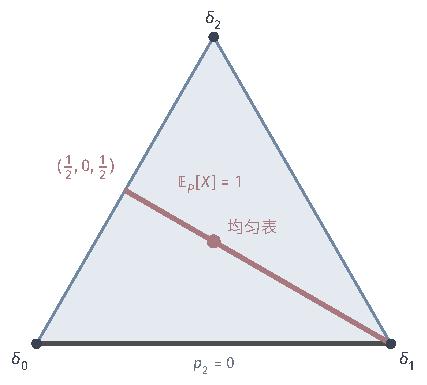
\includegraphics[width=72.4mm]{figures/07-probability/04-distribution-analysis/tikz/dfam-simplex-candidates/figure.pdf}
  \caption{$\{0,1,2\}$上的全体概率表构成三角形$\Delta_2$，三个顶点是点质量$\delta_0,\delta_1,\delta_2$。浅蓝区域是三个结果都有正概率的内部；深灰粗边$p_2=0$是不出现结果$2$的表，也是相对计数测度$\nu$（支撑$\{0,1\}$）绝对连续的表；红色线段是满足$\mathbb{E}_P[X]=1$的表$(t,1-2t,t)$，红点为均匀表。}
  \label{fig:dfam-simplex-candidates}
\end{BookInlineFigure}

第三类要求是相对某个\term{参考测度}（reference measure）$\nu$绝对连续，即凡$\nu(B)=0$的集合都有$P(B)=0$。在$\{0,1,2\}$上取$\nu$为$\{0,1\}$上的计数测度，$\nu(\{2\})=0$，于是$P\ll\nu$恰好意味着$p_2=0$，与固定支持的要求相同。在有限空间上两者没有差别；在连续空间上，绝对连续才保证密度$\mathrm{d}P/\mathrm{d}\nu$存在（Radon–Nikodym定理，见\BookChapterRef{chap:measure-densities}{卷四第8章“测度的密度”}），它是用密度描述分布族的前提。

几类要求可以叠加。同时要求三个结果都可能出现、平均为$1$，候选集合就是去掉两个端点的开线段。每加一条要求，三角形里剩下的部分就小一些，但它仍然是概率表的集合，我们还没有给其中的表起任何名字。

\paragraph{给定均值的密度}
换到连续情形，差别就显出来了。设读数取值于$(0,\infty)$，要求分布相对Lebesgue测度绝对连续且均值为$1$，候选集合是
\begin{equation}
  \mathcal{C}_1=\Bigl\{f\geq0:\int_0^\infty f(x)\,\mathrm{d}x=1,\ \int_0^\infty xf(x)\,\mathrm{d}x=1\Bigr\}.
  \label{eq:dfam-mean-one}
\end{equation}
这里两个密度若几乎处处相等，就看作同一个分布。$\operatorname{Exp}(1)$的密度$\mathrm{e}^{-x}$、$\operatorname{Gamma}(2,2)$的密度$4x\mathrm{e}^{-2x}$和$\operatorname{Unif}(0,2)$的密度$1/2$（$0<x<2$）都在$\mathcal{C}_1$里，形状却各不相同，见图~\ref{fig:dfam-mean-one-densities}。点质量$\delta_1$的均值也是$1$，但它不相对Lebesgue测度绝对连续，被第一个要求排除在外。

\begin{BookInlineFigure}
  \centering
  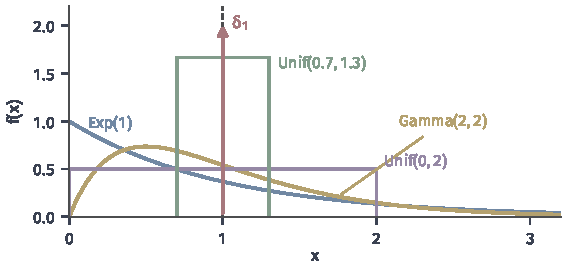
\includegraphics[width=96mm]{figures/07-probability/04-distribution-analysis/matplotlib/dfam-mean-one-densities/figure.pdf}
  \caption{均值都等于$1$的几个分布。蓝线为$\operatorname{Exp}(1)$，黄线为$\operatorname{Gamma}(2,2)$，紫线为$\operatorname{Unif}(0,2)$，绿线为$(1-a,1+a)$上的均匀密度（$a=0.3$）；红色箭头表示点质量$\delta_1$，它没有相对Lebesgue测度的密度。深灰竖线标出均值$x=1$。}
  \label{fig:dfam-mean-one-densities}
\end{BookInlineFigure}

$\mathcal{C}_1$大到什么程度？取$0<a_1<a_2<\cdots<a_n<1$，令$g_k$为区间$(1-a_k,1+a_k)$上的均匀密度。区间关于$1$对称，所以每个$g_k$的均值都是$1$。对任意权重$c_k\geq0$、$\sum_kc_k=1$，凸组合$\sum_kc_kg_k$仍非负、积分为$1$、均值为$1$，所以它也在$\mathcal{C}_1$中。

这$n$个密度线性无关。设$\sum_kc_kg_k=0$几乎处处成立。在区间$(1+a_{n-1},1+a_n)$上只有$g_n$不为零，所以$c_n=0$；去掉$g_n$后对$g_{n-1}$重复同样的论证，依次得到所有$c_k=0$。由于$n$可以任意大，$\mathcal{C}_1$不包含在任何有限维仿射子空间中，因而不能写成有限个固定密度带参数的线性组合。

这说明候选范围与参数表示是两回事。三角形上的线段可以用一个数$t$编号，$\mathcal{C}_1$却不能用有限个系数作线性编号。描述候选集合时不应预设它总有一个有限维参数；有限维的参数族是从候选集合中再挑出的一部分，挑法正是本章后面几节的内容。

\subsection{参数表示与可辨识性}
\label{sec:dfam-identifiability}

给分布编号，就是指定一个集合$\Theta$和一个映射$\bm{\theta}\mapsto P_{\bm{\theta}}$，让每个参数值对应一个概率测度。

\begin{definition}[参数化分布族]
\label{def:dfam-parametric-family}
设$\Theta$是一个集合，对每个$\bm{\theta}\in\Theta$给定$P_{\bm{\theta}}\in\mathcal{P}(\mathcal{X})$。分布族$\{P_{\bm{\theta}}:\bm{\theta}\in\Theta\}$称为以$\Theta$为\term{参数空间}（parameter space）的参数化分布族。若各$P_{\bm{\theta}}$都相对同一个参考测度$\nu$绝对连续，记其密度为$p_{\bm{\theta}}$。
\end{definition}

分布族是映射的像，参数化是映射本身。同一个族可以有许多参数化。Bernoulli族$\{\operatorname{Bern}(p):0<p<1\}$可以直接用$p$编号，也可以用$\eta\in\mathbb{R}$编号：
\[
  p=\frac{\mathrm{e}^{\eta}}{1+\mathrm{e}^{\eta}} .
\]
两种编号得到的分布集合完全相同，对应单纯形$\Delta_1$（一条线段）去掉两个端点，差别只在刻度：$p$在$(0,1)$上均匀刻度，$\eta$把靠近$0$和$1$的部分拉长到整条实轴。

\paragraph{重复的参数}
编号可能是冗余的。令$(a,b)\in(0,\infty)^2$对应$\operatorname{Bern}\bigl(a/(a+b)\bigr)$。$(1,2)$与$(2,4)$给出同一个分布$\operatorname{Bern}(1/3)$；更一般地，从原点出发的每条射线$\{(ca,cb):c>0\}$整条对应同一个分布，如图~\ref{fig:dfam-redundant-parameters}。两个参数，却只描述一个自由度的分布。

\begin{BookInlineFigure}
  \centering
  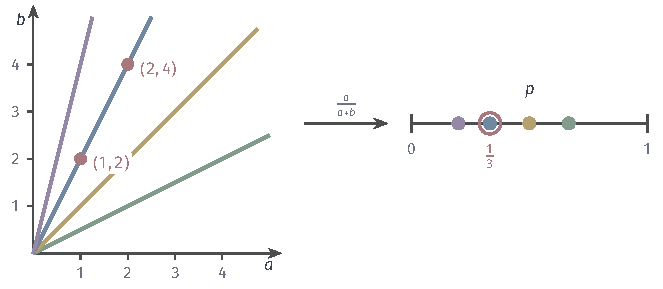
\includegraphics[width=112mm]{figures/07-probability/04-distribution-analysis/tikz/dfam-redundant-parameters/figure.pdf}
  \caption{冗余参数化$(a,b)\mapsto\operatorname{Bern}(a/(a+b))$。左：参数平面中，同一条射线上的点（同色）对应同一个分布，红点$(1,2)$与$(2,4)$都给出$\operatorname{Bern}(1/3)$。右：分布只由$p=a/(a+b)$决定，射线被压成线段$(0,1)$上的一点。}
  \label{fig:dfam-redundant-parameters}
\end{BookInlineFigure}

\begin{definition}[可辨识性]
\label{def:dfam-identifiable}
若对$\bm{\theta},\bm{\theta}'\in\Theta$，由$P_{\bm{\theta}}=P_{\bm{\theta}'}$总能推出$\bm{\theta}=\bm{\theta}'$，则称参数化$\bm{\theta}\mapsto P_{\bm{\theta}}$是\term{可辨识}（identifiable）的。
\end{definition}

可辨识就是参数到分布的映射是单射。这里的“分布相等”指两个概率测度在每个可测集上相等；用密度描述时，指$p_{\bm{\theta}}=p_{\bm{\theta}'}$相对$\nu$几乎处处成立。$\operatorname{Unif}[0,\theta]$与$\operatorname{Unif}(0,\theta)$的密度只在两个端点不同，它们是同一个分布，改动零测集上的值不产生新的参数。

可辨识性是参数化的性质，不是分布族的性质。上面的$(a,b)$参数化不可辨识，同一个Bernoulli族用$p$编号却可辨识。另一个常见的冗余来自参数只以组合形式出现：$(\theta_1,\theta_2)\mapsto\mathcal{N}(\theta_1+\theta_2,1)$中，直线$\theta_1+\theta_2=c$上的所有参数都给出$\mathcal{N}(c,1)$，分布只看得见和，看不见两个加数各是多少。

\paragraph{标签置换}
第~\ref{chap:random-vectors}章的混合分布带来另一种冗余。把两个高斯成分按权重相加，参数是$(w,\mu_1,\mu_2)$：
\[
  P_{(w,\mu_1,\mu_2)}=w\,\mathcal{N}(\mu_1,1)+(1-w)\,\mathcal{N}(\mu_2,1).
\]
交换两个成分的名字，得到
\[
  P_{(0.3,-1,2)}=P_{(0.7,2,-1)} .
\]
两组参数不同，分布却相同，这称为\term{标签置换}（label switching）。图~\ref{fig:dfam-label-switching}在$w=1/2$时画出$(\mu_1,\mu_2)$平面：关于对角线对称的两点给出同一个分布。

\begin{BookInlineFigure}
  \centering
  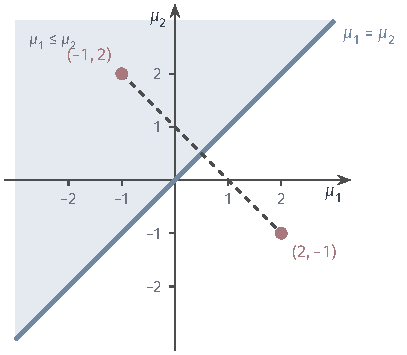
\includegraphics[width=68.9mm]{figures/07-probability/04-distribution-analysis/tikz/dfam-label-switching/figure.pdf}
  \caption{等权两成分高斯混合$\frac12\mathcal{N}(\mu_1,1)+\frac12\mathcal{N}(\mu_2,1)$的参数平面。关于对角线$\mu_1=\mu_2$对称的两点（红点$(-1,2)$与$(2,-1)$）给出同一个分布。限制在浅蓝的半平面$\mu_1\leq\mu_2$中，每个分布只剩一个参数。}
  \label{fig:dfam-label-switching}
\end{BookInlineFigure}

消除这种冗余有两个办法。一是缩小参数空间，例如只保留$\mu_1\leq\mu_2$的参数；二是承认参数只能确定到某种等价，把互相置换的参数看作同一个。两种办法都不改变分布族，只改变编号方式。混合表示中还有更多冗余，第~\ref{sec:dfam-mixture-nonuniqueness}节专门处理。

\paragraph{可辨识与能否从样本分辨}
可辨识性只问两个参数是否给出不同的分布，不问这种差别有多大。$\operatorname{Bern}(0.50)$与$\operatorname{Bern}(0.51)$是两个不同的分布，$p$参数化可辨识；可是各抛$100$次，正面次数的均值分别是$50$与$51$，标准差都约为$5$，两组次数的波动远大于均值之差，看一次试验结果几乎无法判断是哪一个。

另一个例子是$\theta\mapsto\mathcal{N}(\theta^{3},1)$。$\theta\mapsto\theta^{3}$是单射，所以它可辨识；但$\theta=0.1$与$\theta=0$对应的均值只差$0.001$，参数在$0$附近的变化几乎不改变分布。可辨识是分布层面的唯一性，是能否从数据推断参数的前提，但不是充分条件；有限样本下能多准确地估计参数，属于统计推断的问题，见\BookChapterRef{chap:parametric-statistical-inference}{卷八第1章“参数化统计推断”}。


\section{推前构造}
\label{sec:dfam-pushforward}

生成一个$\mathcal{N}(\mu,\sigma^{2})$样本，最省事的做法是先生成标准高斯$Z$，再计算$\mu+\sigma Z$。参数没有进入随机性，只进入了最后那一步计算。把这个做法一般化，就得到构造分布族的第一种办法：随机性由一个固定的基础分布提供，参数只控制把基础样本送到哪里去的映射。

设$(\mathcal{Z},\mathcal{F}_{\mathcal{Z}})$上有一个固定的概率测度$P_0$，$Z\sim P_0$。对每个参数$\bm{\theta}\in\Theta$给定可测映射$T_{\bm{\theta}}:\mathcal{Z}\to\mathcal{X}$，令$X_{\bm{\theta}}=T_{\bm{\theta}}(Z)$。由第~\ref{chap:probability-spaces}章，$X_{\bm{\theta}}$的分布是推前测度$P_{\bm{\theta}}=T_{\bm{\theta}\#}P_0$，即对每个$B\in\mathcal{F}_{\mathcal{X}}$，
\begin{equation}
  P_{\bm{\theta}}(B)=P_0\bigl(T_{\bm{\theta}}^{-1}(B)\bigr).
  \label{eq:dfam-pushforward}
\end{equation}

\begin{definition}[推前族]
\label{def:dfam-pushforward-family}
固定基础分布$P_0$与一族可测映射$\{T_{\bm{\theta}}:\bm{\theta}\in\Theta\}$，由式~\eqref{eq:dfam-pushforward}给出的$\{P_{\bm{\theta}}:\bm{\theta}\in\Theta\}$称为由$P_0$生成的\term{推前族}（pushforward family）。
\end{definition}

用单位质量的图景看，$P_0$把一份质量铺在$\mathcal{Z}$上，$T_{\bm{\theta}}$把每一小份质量搬到它在$\mathcal{X}$中的像；搬完以后落在$B$中的质量，就是原来落在$T_{\bm{\theta}}^{-1}(B)$中的质量。图~\ref{fig:dfam-pushforward-scheme}画出这个结构：基础分布固定，参数只出现在映射上。

\begin{BookInlineFigure}
  \centering
  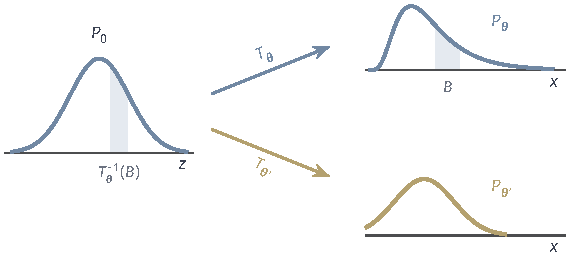
\includegraphics[width=96.6mm]{figures/07-probability/04-distribution-analysis/tikz/dfam-pushforward-scheme/figure.pdf}
  \caption{推前族的结构。左：固定的基础分布$P_0$，浅蓝带是集合$T_{\bm{\theta}}^{-1}(B)$；中间：随参数变化的映射$T_{\bm{\theta}}$；右：输出分布$P_{\bm{\theta}}$，浅蓝带是$B$。两块浅蓝区域的概率相等。两个参数$\bm{\theta}$、$\bm{\theta}'$（蓝、黄）共用同一个$P_0$。}
  \label{fig:dfam-pushforward-scheme}
\end{BookInlineFigure}

这种描述有两个直接的好处。第一，期望可以在基础空间上计算：对使下式一端有意义的可测函数$g$，
\begin{equation}
  \mathbb{E}_{P_{\bm{\theta}}}[g]=\mathbb{E}\bigl[g\bigl(T_{\bm{\theta}}(Z)\bigr)\bigr],
  \label{eq:dfam-pushforward-expectation}
\end{equation}
这是推前测度的积分公式，见\BookChapterRef{chap:pushforward-measures}{卷四第9章“推前测度”}。第二，生成样本只需生成$Z$再算一次映射。两者都不要求$P_{\bm{\theta}}$有密度。

推前构造的表达能力很强。第~\ref{chap:random-variables}章证明，若$U\sim\operatorname{Unif}(0,1)$，$Q$是任一分布函数$F$的分位数函数，则$Q(U)$的分布函数是$F$。所以$\mathbb{R}$上每一个分布都是$\operatorname{Unif}(0,1)$的推前。真正限制一个推前族的，是允许的映射类；下面两小节分别看最简单的映射类，以及映射怎样改变分布的结构。

\subsection{位置尺度族}
\label{sec:dfam-location-scale}

最简单的映射是平移加正向伸缩。第~\ref{chap:common-distributions}章已经用它解释过位置参数与尺度参数，这里把它作为推前族整理一遍，看分布函数、分位数和矩怎样随参数变化。

\begin{definition}[位置尺度族]
\label{def:dfam-location-scale}
设$Z$是实值随机变量，分布为$P_0$。对$\mu\in\mathbb{R}$、$\sigma>0$，令$P_{\mu,\sigma}$为$\mu+\sigma Z$的分布。$\{P_{\mu,\sigma}:\mu\in\mathbb{R},\ \sigma>0\}$称为由$P_0$生成的\term{位置尺度族}（location-scale family）。
\end{definition}

\paragraph{分布函数与分位数}
记$X=\mu+\sigma Z$。由$\sigma>0$，事件$\{X\leq x\}$与$\{Z\leq(x-\mu)/\sigma\}$相同，所以
\begin{equation}
  F_X(x)=F_Z\Bigl(\frac{x-\mu}{\sigma}\Bigr).
  \label{eq:dfam-ls-cdf}
\end{equation}
分布函数的图像只是被横向平移和伸缩。分位数函数的变化方向相反：第~\ref{chap:random-variables}章对$a>0$证明了$aZ+b$的分位数函数是$aQ_Z+b$，取$a=\sigma$、$b=\mu$，得到
\begin{equation}
  Q_X(u)=\mu+\sigma Q_Z(u),\qquad 0<u<1 .
  \label{eq:dfam-ls-quantile}
\end{equation}

式~\eqref{eq:dfam-ls-quantile}对每个$u$都成立，所以中位数、四分位数这些分位数一起按同一个仿射映射变化，四分位距乘以$\sigma$。把$X$的分位数对$Z$的同一水平分位数作图，点$(Q_Z(u),Q_X(u))$全部落在斜率为$\sigma$、截距为$\mu$的直线上。这条直线是检验“$X$是否属于$P_0$生成的位置尺度族”的图形办法，它不需要任何矩存在。

\paragraph{矩与标准化形状}
若$\mathbb{E}\lvert Z\rvert^{k}<\infty$，由凸函数$t\mapsto\lvert t\rvert^{k}$（$k\geq1$）的Jensen不等式，
\[
  \lvert X\rvert^{k}\leq2^{k-1}\bigl(\lvert\mu\rvert^{k}+\sigma^{k}\lvert Z\rvert^{k}\bigr),
\]
所以$X$的$k$阶矩也有限。由期望的线性和方差的缩放规律，
\begin{equation}
  \mathbb{E}[X]=\mu+\sigma\,\mathbb{E}[Z],\qquad\operatorname{Var}(X)=\sigma^{2}\operatorname{Var}(Z).
  \label{eq:dfam-ls-moments}
\end{equation}
矩不存在时，这些式子没有意义，但式~\eqref{eq:dfam-ls-cdf}与式~\eqref{eq:dfam-ls-quantile}照样成立。

再看偏度与峰度这类描述形状的量。设$\operatorname{Var}(Z)>0$，记$m_Z=\mathbb{E}[Z]$，$s_Z$为$Z$的标准差。由式~\eqref{eq:dfam-ls-moments}，$X$的标准化变量是
\[
  \frac{X-\mathbb{E}[X]}{\sqrt{\operatorname{Var}(X)}}=\frac{\sigma(Z-m_Z)}{\sigma s_Z}=\frac{Z-m_Z}{s_Z} .
\]
它与$\mu,\sigma$无关，所以只要相应的矩存在，标准化后的各阶矩，特别是偏度与峰度，在整个位置尺度族中保持不变。

更直接地，$(X-\mu)/\sigma=Z$，把族中任一成员按自己的参数标准化，都回到同一个基础分布。位置与尺度只决定分布放在哪里、铺开多宽，不改变标准化后的形状。

\paragraph{密度}
若$Z$有密度$f_Z$，第~\ref{chap:common-distributions}章已经算出$X$的密度
\begin{equation}
  f_X(x)=\frac{1}{\sigma}\,f_Z\Bigl(\frac{x-\mu}{\sigma}\Bigr).
  \label{eq:dfam-ls-density}
\end{equation}
因子$1/\sigma$来自伸缩：质量不变而区间拉长$\sigma$倍，单位长度上的质量就降为$1/\sigma$。

\paragraph{一个完整的例子}
取基础分布$Z\sim\operatorname{Exp}(1)$。由式~\eqref{eq:dfam-ls-cdf}，$X=\mu+\sigma Z$的分布函数是
\[
  F_X(x)=1-\exp\Bigl(-\frac{x-\mu}{\sigma}\Bigr),\qquad x\geq\mu ,
\]
$x<\mu$时为$0$。它的支撑是$[\mu,\infty)$，左端点随位置参数移动。$Z$的分位数函数是$Q_Z(u)=-\ln(1-u)$，由式~\eqref{eq:dfam-ls-quantile}，
\[
  Q_X(u)=\mu-\sigma\ln(1-u).
\]

取$\mu=1$、$\sigma=2$。中位数与两个四分位数分别是
\[
  Q_X(\tfrac12)=1+2\ln2\approx2.386,\quad Q_X(\tfrac14)\approx1.575,\quad Q_X(\tfrac34)\approx3.773 .
\]
四分位距是$2(\ln4-\ln\tfrac43)=2\ln3\approx2.197$，正好是$Z$的四分位距$\ln3$的$\sigma=2$倍。由式~\eqref{eq:dfam-ls-moments}，均值与方差是
\[
  \mathbb{E}[X]=1+2\cdot1=3,\qquad\operatorname{Var}(X)=4\cdot1=4 .
\]
$\operatorname{Exp}(1)$的偏度是$2$，所以族中每个成员的偏度都是$2$。

图~\ref{fig:dfam-location-scale}(a)画出三组参数的密度，它们看上去宽窄、位置都不同；(b)是分位数对照，三条曲线都是直线，斜率与截距读出$\sigma$与$\mu$。直线的事实说明它们属于同一个位置尺度族，宽窄的差别只是刻度的差别。

\begin{BookInlineFigure}
  \centering
  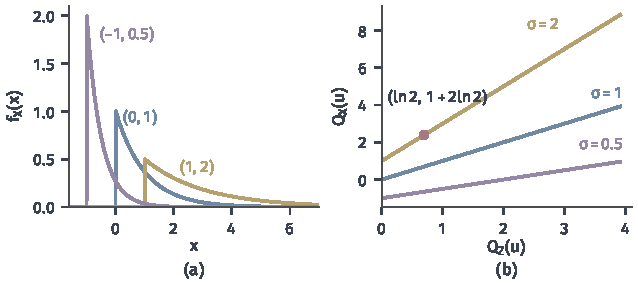
\includegraphics[width=108mm]{figures/07-probability/04-distribution-analysis/matplotlib/dfam-location-scale/figure.pdf}
  \caption{由$\operatorname{Exp}(1)$生成的位置尺度族。(a)$(\mu,\sigma)=(0,1)$（蓝）、$(1,2)$（黄）、$(-1,0.5)$（紫）的密度，支撑的左端点在$x=\mu$。(b)各成员的分位数$Q_X(u)$对基础分位数$Q_Z(u)$作图，$u$取$0.02$到$0.98$，得到斜率$\sigma$、截距$\mu$的直线；红点是$(\mu,\sigma)=(1,2)$的中位数$(\ln2,\ 1+2\ln2)$。}
  \label{fig:dfam-location-scale}
\end{BookInlineFigure}

\paragraph{基础分布的约定与参数的唯一性}
同一个位置尺度族可以由不同的基础分布生成。$\mathcal{N}(0,1)$与$\mathcal{N}(0,4)$生成的族都是全体高斯分布，但在后一种约定下，$\mu+\sigma Z$的标准差是$2\sigma$，同一个数字$\sigma$表示的宽度不同。一般地，$P_0$换成$a+bZ$（$b>0$）的分布，生成的族不变，参数按$(\mu,\sigma)\mapsto(\mu-\sigma a/b,\ \sigma/b)$换算。所以谈论位置和尺度参数的数值时，必须先固定基础分布。

固定基础分布以后，若$Z$不是几乎必然的常数，参数$(\mu,\sigma)$就是可辨识的。这时$Q_Z$不是常函数，可以取$u<v$使$Q_Z(u)<Q_Z(v)$。若$P_{\mu,\sigma}=P_{\mu',\sigma'}$，两者的分位数函数相同，由式~\eqref{eq:dfam-ls-quantile}，
\[
  \mu+\sigma Q_Z(u)=\mu'+\sigma'Q_Z(u),\qquad\mu+\sigma Q_Z(v)=\mu'+\sigma'Q_Z(v).
\]
两式相减得$(\sigma-\sigma')(Q_Z(v)-Q_Z(u))=0$，于是$\sigma=\sigma'$，再代回得$\mu=\mu'$。若$Z$是常数$c$，则$P_{\mu,\sigma}=\delta_{\mu+\sigma c}$，只有和$\mu+\sigma c$可见，参数不可辨识，这正是上一节$\mathcal{N}(\theta_1+\theta_2,1)$那类冗余的极端情形。

\paragraph{没有矩的成员}
Cauchy分布$f_Z(z)=1/(\pi(1+z^{2}))$没有均值。它生成的位置尺度族中，$\mu$不是均值，$\sigma$也不是标准差，但由$F_Z(z)=\tfrac12+\tfrac1\pi\arctan z$得$Q_Z(\tfrac14)=-1$、$Q_Z(\tfrac34)=1$，再由式~\eqref{eq:dfam-ls-quantile}，$\mu$是中位数，四分位距是$2\sigma$。位置尺度族的定义本身只用到映射，矩只是在存在时顺带跟着变化。

这个族的局限也很清楚：它永远改变不了标准化后的形状。由$\mathcal{N}(0,1)$生成的族里没有偏斜的分布，由$\operatorname{Exp}(1)$生成的族里偏度永远是$2$。要改变形状，映射必须不再是仿射的。

\subsection{映射对分布结构的影响}
\label{sec:dfam-map-effects}

仿射映射只做平移和伸缩。一般映射可以把基础分布弯曲、压扁或切碎，相应地改变输出分布的形状、支撑的维数，甚至让连续分布长出点质量。下面依次看三类映射：可逆的非线性映射、降低维数的映射和离散化。

\paragraph{可逆非线性映射改变形状}
取基础变量$Z\sim\mathcal{N}(0,1)$与映射$T_{\mu,\sigma}(z)=\exp(\mu+\sigma z)$，$\sigma>0$。它是$\mathcal{N}(0,1)$生成的位置尺度族再接一个固定的指数函数，输出是第~\ref{chap:random-variable-transformations}章的对数正态分布。指数函数把$\mathbb{R}$一一地送到$(0,\infty)$，导数处处为正，所以可以用一元单调换元公式求密度：
\[
  f_X(x)=\frac{1}{\sigma x}\,\varphi\Bigl(\frac{\ln x-\mu}{\sigma}\Bigr),\qquad x>0 .
\]

参数的角色在这里发生了变化。$X=\mathrm{e}^{\mu}\,(\mathrm{e}^{Z})^{\sigma}$，原来的位置参数$\mu$变成乘法因子$\mathrm{e}^{\mu}$，即对数正态族的尺度参数；原来的尺度参数$\sigma$成了指数$(\mathrm{e}^{Z})^{\sigma}$中的幂次，它改变的是形状。由高斯的矩母函数，
\[
  \mathbb{E}[X^{k}]=\mathrm{e}^{k\mu}\,\mathbb{E}[\mathrm{e}^{k\sigma Z}]=\mathrm{e}^{k\mu+k^{2}\sigma^{2}/2}.
\]
把$k=1,2,3$代入偏度的定义，因子$\mathrm{e}^{\mu}$全部约去，得到对数正态分布的偏度
\[
  (\mathrm{e}^{\sigma^{2}}+2)\sqrt{\mathrm{e}^{\sigma^{2}}-1},
\]
$\sigma=0.25$时约为$0.78$，$\sigma=1$时约为$6.18$。图~\ref{fig:dfam-lognormal-map}(a)画出映射本身：$z$轴上等概率的区间被送到长短悬殊的区间，右侧被拉长，左侧被压缩；(b)是固定$\mu=0$（中位数为$1$）时三个$\sigma$的密度，$\sigma$越大越偏斜。

\begin{BookInlineFigure}
  \centering
  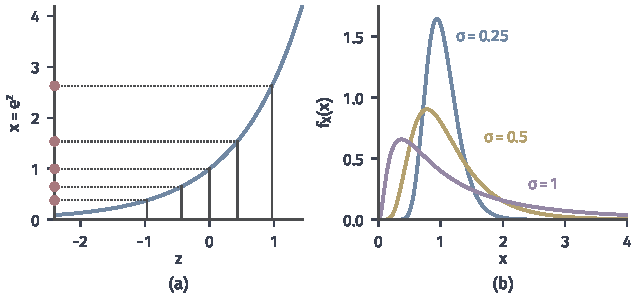
\includegraphics[width=108mm]{figures/07-probability/04-distribution-analysis/matplotlib/dfam-lognormal-map/figure.pdf}
  \caption{可逆非线性映射改变形状。(a)映射$x=\mathrm{e}^{z}$（蓝线）；横轴上深灰竖线把$\mathcal{N}(0,1)$分成六段等概率区间，分点经映射后在纵轴上的位置用红点标出，等概率区间的长度在$x$方向右侧拉长、左侧压缩。(b)$\mu=0$时$\sigma=0.25$（蓝）、$0.5$（黄）、$1$（紫）的对数正态密度，三者中位数都是$1$。}
  \label{fig:dfam-lognormal-map}
\end{BookInlineFigure}

换元公式在这里成立，靠的是映射同维、可逆、连续可微且导数不为零，第~\ref{chap:random-variable-transformations}章与\BookChapterRef{chap:pushforward-measures}{卷四第9章“推前测度”}都要求这些条件。条件破坏时，推前分布依然由式~\eqref{eq:dfam-pushforward}完全确定，只是不再有这样一个公式，甚至根本没有密度。下面两类映射就是这样。

\paragraph{把低维随机性放进高维空间}
取$Z\sim\operatorname{Unif}(0,1)$，参数$r>0$，令
\[
  \bm{X}_r=\bigl(r\cos(2\pi Z),\ r\sin(2\pi Z)\bigr).
\]
$\bm{X}_r$在半径为$r$的圆周上均匀分布，以概率$1$落在圆周上。圆周的平面面积为零，所以$\bm{X}_r$的分布不相对平面Lebesgue测度绝对连续，没有二维密度。参数$r$在这里控制的是支撑本身：不同的$r$给出的分布落在互不相交的圆周上。

这不是圆周的特殊性质。只要输入的维数低于输出，光滑映射的像就是零测集。

\begin{lemma}[低维像的零测性]
\label{lem:dfam-low-dim-image}
设$k<d$，$T:\mathbb{R}^{k}\to\mathbb{R}^{d}$连续可微。则$T(\mathbb{R}^{k})$是$\mathbb{R}^{d}$中的Borel集，且Lebesgue测度为零。因此对$\mathbb{R}^{k}$上任一概率测度$P_0$，$T_\#P_0$都没有相对$d$维Lebesgue测度的密度。
\end{lemma}

\begin{proof}
固定$R>0$，记$K_R=[-R,R]^{k}$。$K_R$是紧凸集，$DT$在$K_R$上连续，所以算子范数有上界$L$。由中值不等式，对$\bm{z},\bm{z}'\in K_R$，
\[
  \lVert T(\bm{z})-T(\bm{z}')\rVert_2\leq L\lVert\bm{z}-\bm{z}'\rVert_2 .
\]

把$K_R$等分成$m^{k}$个边长为$2R/m$的小立方体，每个的直径是$2R\sqrt{k}/m$。它的像落在半径为$2LR\sqrt{k}/m$的球内，从而落在边长为$4LR\sqrt{k}/m$的立方体内。把$m^{k}$块的体积加起来，
\[
  \lambda_d\bigl(T(K_R)\bigr)\leq m^{k}\Bigl(\frac{4LR\sqrt{k}}{m}\Bigr)^{d}=(4LR\sqrt{k})^{d}\,m^{k-d} .
\]
这里$T(K_R)$是紧集的连续像，仍是紧集，所以可测。由$k<d$，令$m\to\infty$，右边趋于零，所以$\lambda_d(T(K_R))=0$。

取$R=1,2,\dots$，$T(\mathbb{R}^{k})=\bigcup_RT(K_R)$是可数个紧集之并，是Borel集，测度为零。$T_\#P_0$在这个零测集上的质量是$P_0(\mathbb{R}^{k})=1$，所以它不相对$\lambda_d$绝对连续，没有密度。
\end{proof}

降维的方向相反时情况不同。$\bm{Z}\sim\mathcal{N}(\bm{0},\bm{I}_2)$，$X=Z_1+Z_2$把两个坐标并成一个，输出有密度，它是$\mathcal{N}(0,2)$；但这个密度不能用同维换元求得，要沿被合并的方向积分，即第~\ref{chap:random-variable-transformations}章的卷积。决定有没有密度的不是输入输出的维数谁大，而是映射是否把正的质量压进输出空间的零测集。线性映射$\bm{X}=\bm{A}\bm{Z}$中$\bm{A}$为奇异的$2\times2$矩阵时，像是一条直线，正是第~\ref{chap:multivariate-distributions}章退化高斯的情形。

\paragraph{离散化产生原子}
第三类映射把连续值归到有限或可数个格子里。取$Z\sim\mathcal{N}(0,1)$，位置参数$\mu$，令$X=\operatorname{round}(\mu+Z)$为最接近$\mu+Z$的整数（半整数处的取法不影响分布，因为那是零概率事件）。$X=k$当且仅当$k-\tfrac12\leq\mu+Z<k+\tfrac12$，所以
\begin{equation}
  \mathbb{P}(X=k)=\Phi\bigl(k+\tfrac12-\mu\bigr)-\Phi\bigl(k-\tfrac12-\mu\bigr),\qquad k\in\mathbb{Z}.
  \label{eq:dfam-rounding}
\end{equation}
连续的基础分布被推成一张概率表。取$\mu=0.3$，代入式~\eqref{eq:dfam-rounding}，
\[
  \mathbb{P}(X=-1)\approx0.176,\quad\mathbb{P}(X=0)\approx0.367,\quad\mathbb{P}(X=1)\approx0.306 .
\]

离散化也可以只作用在一部分取值上。令$X=\max(\mu+Z,0)$，负的读数都记成$0$。$\{X=0\}=\{Z\leq-\mu\}$，于是$\mathbb{P}(X=0)=\Phi(-\mu)$，$X$在$0$处有一个原子；在$(0,\infty)$上$X=\mu+Z$，有密度$\varphi(x-\mu)$。这个分布既不是概率表，也没有相对Lebesgue测度的密度。若取参考测度$\nu=\delta_0+\lambda_1$，它相对$\nu$的密度是
\[
  p(0)=\Phi(-\mu),\qquad p(x)=\varphi(x-\mu)\quad(x>0).
\]
$\mu=0.5$时原子的质量是$\Phi(-0.5)\approx0.309$。

\begin{BookInlineFigure}
  \centering
  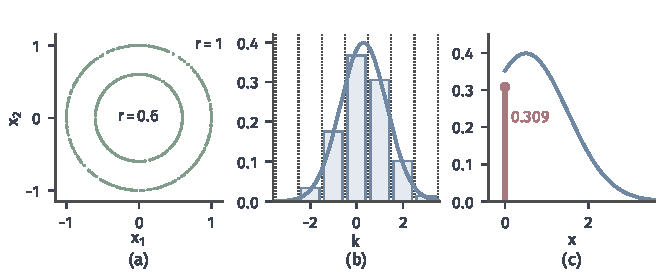
\includegraphics[width=112mm]{figures/07-probability/04-distribution-analysis/matplotlib/dfam-map-effects/figure.pdf}
  \caption{映射改变支撑与类型。(a)$Z\sim\operatorname{Unif}(0,1)$经$z\mapsto r(\cos2\pi z,\sin2\pi z)$得到的$400$个点（绿），$r=1$与$r=0.6$；分布全部落在圆周上，没有平面密度。(b)$\mu=0.3$时$\operatorname{round}(\mu+Z)$的概率表（浅蓝柱），蓝线是$\mu+Z$的密度，深灰竖线是格子边界$k\pm\tfrac12$。(c)$\max(\mu+Z,0)$，$\mu=0.5$：$(0,\infty)$上的密度（蓝线）与$0$处质量$0.309$的原子（红色竖线）。}
  \label{fig:dfam-map-effects}
\end{BookInlineFigure}

图~\ref{fig:dfam-map-effects}把三种结构放在一起。圆周上的分布支撑退化，取整得到概率表，截断得到原子与密度并存的混合类型。三者都是从有密度的基础分布出发、经过可测映射得到的，所以推前族的成员可以有任何类型；只有在同维可逆光滑的情形，才能放心地把它写成一个普通的密度模型。描述一般推前族时，应当用式~\eqref{eq:dfam-pushforward}和式~\eqref{eq:dfam-pushforward-expectation}，而不是先假定存在密度。


\section{混合分布}
\label{sec:dfam-mixtures}

一批零件来自两条生产线，一条偏大、一条偏小，混在一起测量，直方图上会出现两个峰。单个高斯分布无论怎样平移伸缩都只有一个峰，推前一个固定的高斯也不自然。更直接的描述是照着来源写：先随机决定零件来自哪条线，再按那条线的规律产生尺寸。这样得到的分布族，参数分成两类：选择成分的规律，以及各成分自己的参数。

\subsection{有限混合}
\label{sec:dfam-finite-mixture}

设$P_1,\dots,P_m$是$\mathcal{X}$上的概率测度，$\bm{w}=(w_1,\dots,w_m)$是一张概率表。先抽成分指标$K$，$\mathbb{P}(K=k)=w_k$；再在$K=k$的条件下让$X\sim P_k$。由第~\ref{chap:conditional-distributions}章的全概率公式，
\[
  \begin{aligned}
    \mathbb{P}(X\in B)&=\sum_{k=1}^{m}\mathbb{P}(K=k)\,\mathbb{P}(X\in B\mid K=k)\\
    &=\sum_{k=1}^{m}w_kP_k(B).
  \end{aligned}
\]

\begin{definition}[有限混合]
\label{def:dfam-finite-mixture}
设$\bm{w}\in\Delta_{m-1}$，$P_1,\dots,P_m\in\mathcal{P}(\mathcal{X})$。概率测度
\begin{equation}
  P=\sum_{k=1}^{m}w_kP_k
  \label{eq:dfam-finite-mixture}
\end{equation}
称为成分$P_1,\dots,P_m$以\term{混合权重}（mixture weights）$\bm{w}$构成的\term{有限混合}（finite mixture）。若各成分取自一个参数化族，$P_k=Q_{\bm{\eta}_k}$，则混合族的参数是$(\bm{w},\bm{\eta}_1,\dots,\bm{\eta}_m)$。
\end{definition}

式~\eqref{eq:dfam-finite-mixture}是概率的加权平均，对每个事件逐一成立。所以分布函数、密度（若各成分相对同一个$\nu$有密度$p_k$）和有限的期望都按同样的权重相加：
\[
  F=\sum_kw_kF_k,\qquad p=\sum_kw_kp_k,\qquad\mathbb{E}_P[g]=\sum_kw_k\,\mathbb{E}_{P_k}[g].
\]
分位数不在其列。分位数函数是分布函数的广义逆，逆运算与加权平均不能交换，混合的中位数一般不等于各成分中位数的加权平均。

\paragraph{均值与方差}
设第$k$个成分的均值与方差为$m_k$、$s_k^{2}$，记$\bar{m}=\sum_kw_km_k$。由上式，$\mathbb{E}[X]=\bar{m}$。方差由全方差公式（第~\ref{chap:conditional-expectation}章）给出，其中两个条件量是
\[
  \mathbb{E}[X\mid K]=m_K,\qquad\operatorname{Var}(X\mid K)=s_K^{2},
\]
代入得到
\begin{equation}
  \operatorname{Var}(X)=\sum_{k}w_ks_k^{2}+\sum_kw_k(m_k-\bar{m})^{2}.
  \label{eq:dfam-mixture-variance}
\end{equation}
第一项是成分内部的平均波动，第二项是成分中心之间的分散。若把各成分看成放在$m_k$处的质量块，第二项正是这组质量块绕总重心的转动惯量。

\paragraph{两个高斯成分}
取等权的两个成分$\mathcal{N}(-a,1)$与$\mathcal{N}(a,1)$，$a>0$，混合密度是
\[
  f_a(x)=\tfrac12\varphi(x+a)+\tfrac12\varphi(x-a).
\]
由式~\eqref{eq:dfam-mixture-variance}，均值是$0$，方差是$1+a^{2}$。取$a=1.5$，方差是$3.25$，比每个成分的方差$1$大得多，多出的$2.25$全部来自两个中心的分离。

$f_a$关于$0$对称，所以$f_a'(0)=0$。要判断$0$处是峰还是谷，看二阶导数。$\varphi'(z)=-z\varphi(z)$，再求一次导，
\[
  \varphi''(z)=(z^{2}-1)\varphi(z).
\]
代入$f_a$，两项在$x=0$处相等，得到
\begin{equation}
  f_a''(0)=(a^{2}-1)\,\varphi(a).
  \label{eq:dfam-mixture-curvature}
\end{equation}

$a<1$时$f_a''(0)<0$，中心是局部极大；$a>1$时$f_a''(0)>0$，中心变成局部极小。后一种情形下$f_a$在$0$处是谷，又在$\pm\infty$处趋于零，所以两侧各有一个峰，密度至少有两个峰。$a=1$是转折点，两个成分中心相距$2$，恰为成分标准差的两倍。图~\ref{fig:dfam-mixture-separation}画出$a=0.5,1,1.5,2$的情形。

\begin{BookInlineFigure}
  \centering
  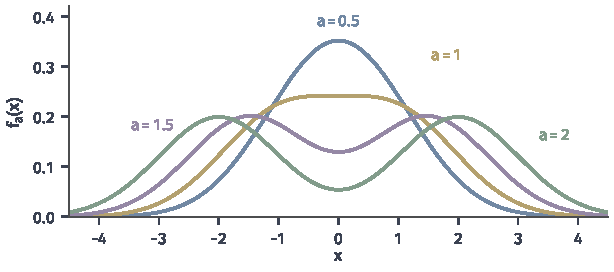
\includegraphics[width=104mm]{figures/07-probability/04-distribution-analysis/matplotlib/dfam-mixture-separation/figure.pdf}
  \caption{等权混合$\frac12\mathcal{N}(-a,1)+\frac12\mathcal{N}(a,1)$的密度，$a=0.5$（蓝）、$1$（黄）、$1.5$（紫）、$2$（绿）。$a=1$时中心处的二阶导数为零，顶部最平；$a>1$时中心是谷，出现两个峰。}
  \label{fig:dfam-mixture-separation}
\end{BookInlineFigure}

单个高斯分布的密度从中心向两侧单调下降，只有一个峰；$\mathcal{N}(0,1)$生成的位置尺度族中所有成员都是如此。两个高斯的混合却能有两个峰。这是混合族比它的成分族多出来的形状。

\paragraph{只改权重与改变成分}
混合族的两类参数作用不同。固定成分只改权重，密度$p=\sum_kw_kp_k$对$\bm{w}$是线性的：权重把质量在几块固定的形状之间重新分配，峰的位置大体不动，峰的高低此消彼长。全体权重给出的分布构成一个凸集，第~\ref{sec:dfam-candidates}节三角形中的线段就是两个概率表的全部混合。

改变成分参数则改变形状本身，密度对它们是非线性的。图~\ref{fig:dfam-mixture-weights-params}(a)固定$a=1.5$，把第二个成分的权重从$0.5$增到$0.9$，右峰升高、左峰缩成肩部；(b)固定等权，把第二个成分的标准差缩小到$0.5$、中心移到$2$，右峰变得又窄又高，左峰的形状不变。

\begin{BookInlineFigure}
  \centering
  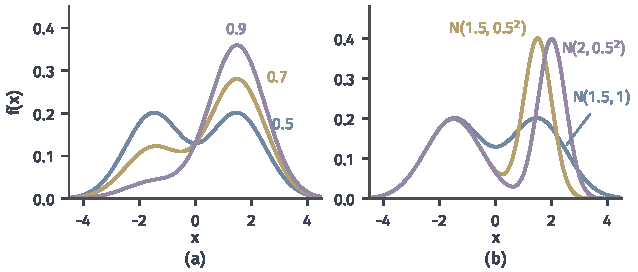
\includegraphics[width=108mm]{figures/07-probability/04-distribution-analysis/matplotlib/dfam-mixture-weights-params/figure.pdf}
  \caption{混合族中两类参数的作用。(a)成分固定为$\mathcal{N}(-1.5,1)$与$\mathcal{N}(1.5,1)$，第二个成分的权重为$0.5$（蓝）、$0.7$（黄）、$0.9$（紫）。(b)等权，第二个成分为$\mathcal{N}(1.5,1)$（蓝）、$\mathcal{N}(1.5,0.5^{2})$（黄）、$\mathcal{N}(2,0.5^{2})$（紫）；第一个成分始终是$\mathcal{N}(-1.5,1)$。}
  \label{fig:dfam-mixture-weights-params}
\end{BookInlineFigure}

\paragraph{混合不是取值的平均}
“按权重$\tfrac12,\tfrac12$组合两个随机量”有两种截然不同的意思。设$Y_1\sim\mathcal{N}(-1.5,1)$与$Y_2\sim\mathcal{N}(1.5,1)$独立。混合是以概率$\tfrac12$报告$Y_1$、以概率$\tfrac12$报告$Y_2$，分布是$f_{1.5}$，方差$3.25$。取值的平均$\tfrac12Y_1+\tfrac12Y_2$则是两个独立高斯的线性组合，由第~\ref{chap:multivariate-distributions}章，它服从
\[
  \mathcal{N}\bigl(0,\ \tfrac14+\tfrac14\bigr)=\mathcal{N}(0,0.5).
\]
它只有一个峰，方差只有$0.5$。

两者的差别在于加权的对象。混合对概率加权，每次只取一个成分的值，两个峰都保留下来；取值平均对随机变量加权，每次都把两个值折中，正负偏离互相抵消。图~\ref{fig:dfam-mix-vs-sum}并排画出两者。

\begin{BookInlineFigure}
  \centering
  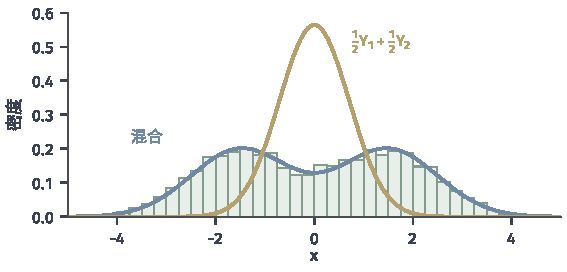
\includegraphics[width=96mm]{figures/07-probability/04-distribution-analysis/matplotlib/dfam-mix-vs-sum/figure.pdf}
  \caption{同一对成分$\mathcal{N}(-1.5,1)$、$\mathcal{N}(1.5,1)$的两种“等权组合”。蓝线是混合$\frac12\mathcal{N}(-1.5,1)+\frac12\mathcal{N}(1.5,1)$，方差$3.25$；黄线是独立变量的平均$\frac12Y_1+\frac12Y_2\sim\mathcal{N}(0,0.5)$。绿色直方图是混合的$5000$个模拟样本（种子$716$）。}
  \label{fig:dfam-mix-vs-sum}
\end{BookInlineFigure}

\subsection{连续混合}
\label{sec:dfam-continuous-mixture}

有限混合的成分指标只取有限个值。若影响结果的隐藏因素是连续的，例如每个零件的加工精度都略有不同，就要让成分由一个连续变量$S$索引。给定$S=s$时，$X$的条件分布是$K(s,\cdot)$；$S$本身服从分布$M$。

\begin{definition}[一般混合]
\label{def:dfam-general-mixture}
设$(\mathcal{S},\mathcal{F}_{\mathcal{S}})$上有概率测度$M$，$K$是从$\mathcal{S}$到$\mathcal{X}$的概率核。概率测度
\begin{equation}
  P(B)=\int_{\mathcal{S}}K(s,B)\,M(\mathrm{d}s),\qquad B\in\mathcal{F}_{\mathcal{X}},
  \label{eq:dfam-general-mixture}
\end{equation}
称为核$K$以\term{混合测度}（mixing measure）$M$构成的混合。$M$不是离散分布时，常称为\term{连续混合}（continuous mixture）。
\end{definition}

$P$确实是概率测度：$K(s,\mathcal{X})=1$给出$P(\mathcal{X})=1$；对互不相交的$B_1,B_2,\dots$，$K(s,\cdot)$可数可加，再由单调收敛定理交换求和与积分，得到$P$可数可加。式~\eqref{eq:dfam-general-mixture}正是第~\ref{chap:conditional-distributions}章由边缘分布与条件分布恢复$X$的边缘分布的公式，这里把它反过来用作构造。取$M=\sum_kw_k\delta_k$，积分退回求和，得到式~\eqref{eq:dfam-finite-mixture}。

若每个$K(s,\cdot)$相对同一个$\nu$有密度$k(x\mid s)$，且$k$对$(s,x)$联合可测，则由Tonelli定理交换积分次序，
\[
  P(B)=\int_{\mathcal{S}}\int_Bk(x\mid s)\,\nu(\mathrm{d}x)\,M(\mathrm{d}s)=\int_B\Bigl(\int_{\mathcal{S}}k(x\mid s)\,M(\mathrm{d}s)\Bigr)\nu(\mathrm{d}x).
\]
所以混合的密度是条件密度按$M$的平均：
\begin{equation}
  p(x)=\int_{\mathcal{S}}k(x\mid s)\,M(\mathrm{d}s).
  \label{eq:dfam-mixture-density}
\end{equation}

\paragraph{正态尺度混合}
最常用的连续混合是第~\ref{chap:multivariate-distributions}章的正态尺度混合：$W\geq0$与$Z\sim\mathcal{N}(0,1)$独立，$X=\sqrt{W}Z$。给定$W=w$，$X\sim\mathcal{N}(0,w)$，混合测度是$W$的分布。那一章用它构造了t分布与Laplace分布；这里关心的是，不管$W$怎样分布，混合都带来什么共同的形状。

\begin{theorem}[尺度混合使峰度不小于三]
\label{thm:dfam-scale-mixture-kurtosis}
设$W\geq0$，$\mathbb{E}[W^{2}]<\infty$，$\mathbb{P}(W>0)>0$，$Z\sim\mathcal{N}(0,1)$与$W$独立，$X=\sqrt{W}Z$。则$X$的峰度
\begin{equation}
  \kappa(X)=\frac{\mathbb{E}[X^{4}]}{(\mathbb{E}[X^{2}])^{2}}=\frac{3\,\mathbb{E}[W^{2}]}{(\mathbb{E}[W])^{2}}\geq3 ,
  \label{eq:dfam-scale-kurtosis}
\end{equation}
等号成立当且仅当$W$几乎必然为常数。
\end{theorem}

\begin{proof}
$X$的均值是$\mathbb{E}[\sqrt{W}]\,\mathbb{E}[Z]=0$。由独立性与$\mathbb{E}[Z^{2}]=1$、$\mathbb{E}[Z^{4}]=3$，
\[
  \mathbb{E}[X^{2}]=\mathbb{E}[W]\,\mathbb{E}[Z^{2}]=\mathbb{E}[W],\qquad\mathbb{E}[X^{4}]=\mathbb{E}[W^{2}]\,\mathbb{E}[Z^{4}]=3\,\mathbb{E}[W^{2}].
\]
由$\mathbb{P}(W>0)>0$，$\mathbb{E}[W]>0$，比值有意义。由方差非负，
\[
  \mathbb{E}[W^{2}]-(\mathbb{E}[W])^{2}=\operatorname{Var}(W)\geq0 ,
\]
所以$\kappa(X)\geq3$；等号成立当且仅当$\operatorname{Var}(W)=0$，即$W$几乎必然等于常数。
\end{proof}

高斯分布的峰度恰好是$3$。定理说，只要尺度真的随机，混合的峰度就严格大于$3$：大的$W$贡献远处的值，小的$W$贡献贴近$0$的值，结果比同方差的高斯分布中间更尖、尾部更厚。例如$W$以各$\tfrac12$的概率取$0.5$和$1.5$，这是两成分的有限混合，
\[
  \mathbb{E}[W]=1,\qquad\mathbb{E}[W^{2}]=\tfrac12(0.25+2.25)=1.25,\qquad\kappa(X)=3.75 .
\]
取$W\sim\operatorname{Exp}(1)$，$\mathbb{E}[W]=1$，$\mathbb{E}[W^{2}]=2$，由式~\eqref{eq:dfam-scale-kurtosis}得$\kappa(X)=6$；第~\ref{chap:multivariate-distributions}章算出这时$X$服从$\operatorname{Laplace}(0,1/\sqrt2)$，其峰度正是$6$。

\paragraph{共同尺度带来的依赖}
在多元情形，同一个$W$乘到所有分量上。设$\bm{Z}\sim\mathcal{N}(\bm{0},\bm{I}_2)$与$W$独立，$\bm{X}=\sqrt{W}\bm{Z}$，$\mathbb{E}[W^{2}]<\infty$。由独立性，
\[
  \operatorname{Cov}(\bm{X})=\mathbb{E}[W]\,\bm{I}_2 ,
\]
两个分量不相关。但它们不独立：
\[
  \mathbb{E}[X_1^{2}X_2^{2}]=\mathbb{E}[W^{2}]\,\mathbb{E}[Z_1^{2}]\,\mathbb{E}[Z_2^{2}]=\mathbb{E}[W^{2}],
\]
而两个边缘二阶矩的乘积是
\[
  \mathbb{E}[X_1^{2}]\,\mathbb{E}[X_2^{2}]=(\mathbb{E}[W])^{2}.
\]
若$W$不是常数，两者不等，$X_1^{2}$与$X_2^{2}$正相关，所以$X_1,X_2$不独立。$W\sim\operatorname{Exp}(1)$时
\[
  \operatorname{Cov}(X_1^{2},X_2^{2})=\mathbb{E}[W^{2}]-(\mathbb{E}[W])^{2}=1 .
\]

直观上，$W$大的那一次，两个分量同时被放大；$W$小的那一次，两个分量同时贴近原点。图~\ref{fig:dfam-scale-mixture}(b)中，离原点较远的点（红）均匀地散在各个方向上，包括对角方向，说明两个分量常常一起取大值；(c)让每个分量各用一个独立的$W_i$，边缘分布与(b)完全相同，远处的点却集中在两条坐标轴附近：一个分量很大时，另一个分量通常仍然不大。只看边缘分布或协方差，分不出这两种模型。

\begin{BookInlineFigure}
  \centering
  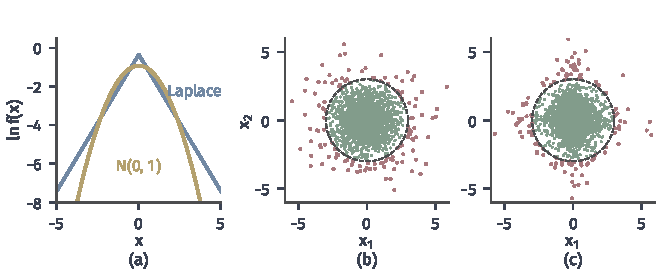
\includegraphics[width=112mm]{figures/07-probability/04-distribution-analysis/matplotlib/dfam-scale-mixture/figure.pdf}
  \caption{正态尺度混合，$W\sim\operatorname{Exp}(1)$。(a)一元密度的对数：$X=\sqrt{W}Z$即$\operatorname{Laplace}(0,1/\sqrt2)$（蓝），与同方差的$\mathcal{N}(0,1)$（黄）；混合的中心更尖、尾部按直线而非抛物线下降。(b)共同尺度$\sqrt{W}(Z_1,Z_2)$的$3000$个样本。(c)独立尺度$(\sqrt{W_1}Z_1,\sqrt{W_2}Z_2)$的$3000$个样本。(b)(c)中深灰虚线是半径$3$的圆，圆外的点标红；两图的边缘分布相同，协方差都是$\bm{I}_2$；模拟种子$716$。}
  \label{fig:dfam-scale-mixture}
\end{BookInlineFigure}

\paragraph{计数的混合}
连续混合同样适用于离散结果。设给定$\Lambda=\lambda$时$X\sim\operatorname{Poisson}(\lambda)$，而强度$\Lambda\sim\operatorname{Gamma}(\alpha,\beta)$。由式~\eqref{eq:dfam-mixture-density}，以计数测度为参考，
\[
  \mathbb{P}(X=k)=\int_0^\infty\mathrm{e}^{-\lambda}\frac{\lambda^{k}}{k!}\cdot\frac{\beta^{\alpha}\lambda^{\alpha-1}\mathrm{e}^{-\beta\lambda}}{\Gamma(\alpha)}\,\mathrm{d}\lambda .
\]

把$\lambda$的幂与指数合并，剩下的积分是一个Gamma积分，
\[
  \int_0^\infty\lambda^{k+\alpha-1}\mathrm{e}^{-(1+\beta)\lambda}\,\mathrm{d}\lambda=\frac{\Gamma(k+\alpha)}{(1+\beta)^{k+\alpha}} .
\]
代回得到
\begin{equation}
  \mathbb{P}(X=k)=\frac{\Gamma(k+\alpha)}{k!\,\Gamma(\alpha)}\Bigl(\frac{\beta}{1+\beta}\Bigr)^{\alpha}\Bigl(\frac{1}{1+\beta}\Bigr)^{k},\qquad k=0,1,\dots
  \label{eq:dfam-negative-binomial}
\end{equation}
这是\term{负二项分布}（negative binomial distribution）。

取$\alpha=2$、$\beta=1$，式~\eqref{eq:dfam-negative-binomial}化为$\mathbb{P}(X=k)=(k+1)/2^{k+2}$，前几项是
\[
  p_0=\tfrac14,\quad p_1=\tfrac14,\quad p_2=\tfrac{3}{16},\quad p_3=\tfrac18 .
\]
均值由全期望公式得$\mathbb{E}[\Lambda]=\alpha/\beta=2$，与$\operatorname{Poisson}(2)$相同。方差由全方差公式得
\[
  \operatorname{Var}(X)=\mathbb{E}[\Lambda]+\operatorname{Var}(\Lambda)=\frac{\alpha}{\beta}+\frac{\alpha}{\beta^{2}}=4 ,
\]
是$\operatorname{Poisson}(2)$方差的两倍。强度的随机性使$0$和大计数都更常见：$p_0=0.25$，而$\operatorname{Poisson}(2)$在$0$处只有$\mathrm{e}^{-2}\approx0.135$，见图~\ref{fig:dfam-poisson-gamma}。

\begin{BookInlineFigure}
  \centering
  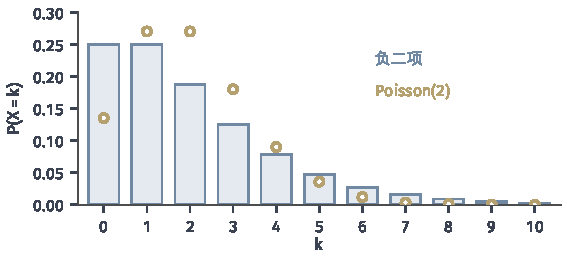
\includegraphics[width=96mm]{figures/07-probability/04-distribution-analysis/matplotlib/dfam-poisson-gamma/figure.pdf}
  \caption{计数的连续混合。浅蓝柱是$\operatorname{Poisson}(\Lambda)$、$\Lambda\sim\operatorname{Gamma}(2,1)$的混合，即负二项分布$(k+1)/2^{k+2}$；黄色空心点是同均值的$\operatorname{Poisson}(2)$。两者均值都是$2$，方差分别为$4$与$2$。}
  \label{fig:dfam-poisson-gamma}
\end{BookInlineFigure}

\paragraph{改变混合测度与改变核}
连续混合族有两个可以变动的部分。固定核$K(w,\cdot)=\mathcal{N}(0,w)$，让混合测度$M$取遍$(0,\infty)$上全体概率测度，得到全体正态尺度混合。这个族是凸的，包含所有t分布与上面的Laplace分布，远比任何有限维族大；但它的成员都关于$0$对称，由定理~\ref{thm:dfam-scale-mixture-kurtosis}，四阶矩有限的成员峰度都不小于$3$。

所以改变$M$无论怎样都造不出偏斜的分布，也造不出比高斯更“平”的分布。$\operatorname{Unif}(-\sqrt3,\sqrt3)$的方差为$1$，峰度为$1.8$，它就不是任何正态尺度混合。要得到这些形状，必须换掉核：例如把$\mathcal{N}(0,w)$换成$\mathcal{N}(s,1)$，让混合测度作用在位置上，或者像Poisson–Gamma那样换成离散的核。混合测度决定成分怎样搭配，核决定可以搭配的成分是什么形状。

\subsection{混合表示的非唯一性}
\label{sec:dfam-mixture-nonuniqueness}

混合族的参数比分布多出很多冗余。第~\ref{sec:dfam-identifiability}节已经看到标签置换；这里把各种冗余列清楚，再说明成分互相重叠并不是冗余。

\paragraph{冗余从哪里来}
考虑等方差的两成分高斯混合
\[
  P_{(w,\mu_1,\mu_2)}=w\,\mathcal{N}(\mu_1,1)+(1-w)\,\mathcal{N}(\mu_2,1),\qquad 0\leq w\leq1 .
\]
第一种冗余是标签置换：$(w,\mu_1,\mu_2)$与$(1-w,\mu_2,\mu_1)$给出同一个分布。它把参数成对地粘在一起，每个真正的两成分分布恰好对应两组参数。

第二种冗余来自重复成分。$\mu_1=\mu_2=\mu$时，两个成分相同，
\[
  w\,\mathcal{N}(\mu,1)+(1-w)\,\mathcal{N}(\mu,1)=\mathcal{N}(\mu,1)
\]
对每个$w\in[0,1]$成立，权重完全看不见。第三种冗余来自零权重：$w=0$时，$\mu_1$不出现在分布中，可以取任意值。

以$\mathcal{N}(0,1)$为例，它的全部表示是
\[
  \{w\in[0,1],\ \mu_1=\mu_2=0\}\cup\{w=0,\ \mu_2=0\}\cup\{w=1,\ \mu_1=0\}.
\]
这是参数空间中的三条线段（其中两条是整条直线），不再是孤立的点。图~\ref{fig:dfam-mixture-fibers}(a)在$\mu_2=0$的截面上画出其中两条：$\mu_1=0$的竖线与$w=0$的横线交成一个十字。

\begin{BookInlineFigure}
  \centering
  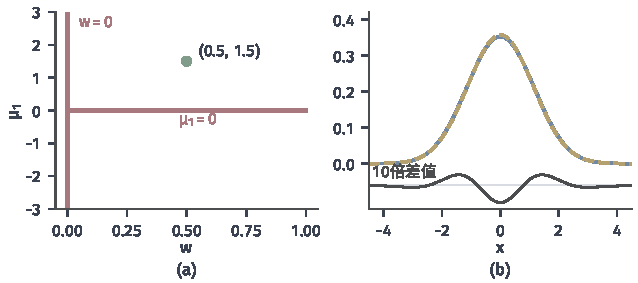
\includegraphics[width=108mm]{figures/07-probability/04-distribution-analysis/matplotlib/dfam-mixture-fibers/figure.pdf}
  \caption{混合表示的冗余与重叠。(a)$\mu_2=0$的截面$(w,\mu_1)$中，给出$\mathcal{N}(0,1)$的参数（红线）：$\mu_1=0$时任何$w$都可以，$w=0$时任何$\mu_1$都可以；绿点是$(0.5,1.5)$，代表一个真正的两成分混合，它在这个截面上只出现一次。(b)重叠很大的混合$\frac12\mathcal{N}(-0.5,1)+\frac12\mathcal{N}(0.5,1)$（蓝）与同均值、同方差的$\mathcal{N}(0,1.25)$（黄）；下方深灰线是两者密度之差，放大$10$倍。}
  \label{fig:dfam-mixture-fibers}
\end{BookInlineFigure}

\paragraph{重叠不等于不可辨识}
成分互相重叠是另一回事。$\tfrac12\mathcal{N}(-0.5,1)+\tfrac12\mathcal{N}(0.5,1)$的两个成分大部分重合，混合只有一个峰，看上去几乎就是一个高斯：图~\ref{fig:dfam-mixture-fibers}(b)中它与同均值同方差的$\mathcal{N}(0,1.25)$的密度之差最大不到$0.005$，约为峰高的$1.4\%$。但两者是不同的分布，而且下面的定理说明，这个混合的参数除了标签置换外是唯一确定的。

记$\varphi_\sigma(x)=\varphi(x/\sigma)/\sigma$为$\mathcal{N}(0,\sigma^{2})$的密度。证明要用到一个关于指数函数的事实。

\begin{lemma}[不同指数的指数函数线性无关]
\label{lem:dfam-exp-independent}
设$\nu_1>\nu_2>\cdots>\nu_r$为实数，$c_1,\dots,c_r$为实数。若对一切$t\in\mathbb{R}$有$\sum_{j=1}^{r}c_j\mathrm{e}^{\nu_jt}=0$，则$c_1=\cdots=c_r=0$。
\end{lemma}

\begin{proof}
两边乘以$\mathrm{e}^{-\nu_1t}$，得
\[
  c_1+\sum_{j=2}^{r}c_j\mathrm{e}^{(\nu_j-\nu_1)t}=0 .
\]
各$\nu_j-\nu_1<0$，令$t\to+\infty$，求和项趋于零，所以$c_1=0$。对剩下的$r-1$项重复这一步，依次得到$c_2=\cdots=c_r=0$。
\end{proof}

\begin{theorem}[已知方差的高斯位置混合可辨识]
\label{thm:dfam-gaussian-mixture-identifiable}
固定$\sigma>0$。设$\mu_1,\dots,\mu_m$互不相同，$\mu'_1,\dots,\mu'_{m'}$互不相同，权重$w_k>0$、$w'_l>0$且各自和为$1$。若
\begin{equation}
  \sum_{k=1}^{m}w_k\,\mathcal{N}(\mu_k,\sigma^{2})=\sum_{l=1}^{m'}w'_l\,\mathcal{N}(\mu'_l,\sigma^{2}),
  \label{eq:dfam-mixture-equal}
\end{equation}
则$m=m'$，且存在$\{1,\dots,m\}$的置换$\pi$，使$\mu'_{\pi(k)}=\mu_k$、$w'_{\pi(k)}=w_k$。
\end{theorem}

\begin{proof}
两边是同一个分布，所以对一切$t$，$\mathrm{e}^{tX}$在两边的期望相同。$\mathcal{N}(\mu,\sigma^{2})$的矩母函数是$\mathrm{e}^{\mu t+\sigma^{2}t^{2}/2}$，有限混合的矩母函数是成分矩母函数的加权和，于是
\[
  \mathrm{e}^{\sigma^{2}t^{2}/2}\sum_{k}w_k\mathrm{e}^{\mu_kt}=\mathrm{e}^{\sigma^{2}t^{2}/2}\sum_{l}w'_l\mathrm{e}^{\mu'_lt},\qquad t\in\mathbb{R}.
\]
约去公共因子$\mathrm{e}^{\sigma^{2}t^{2}/2}>0$，移项，
\[
  \sum_{k}w_k\mathrm{e}^{\mu_kt}-\sum_lw'_l\mathrm{e}^{\mu'_lt}=0,\qquad t\in\mathbb{R}.
\]

把两组位置合在一起，按不同的值合并同类项。对每个出现过的值$\nu$，它的系数是“$\nu$在左边的权重”减去“$\nu$在右边的权重”，在一边没有出现时那一边记为零。由引理~\ref{lem:dfam-exp-independent}，每个系数都为零。若某个$\mu_k$不在右边出现，它的系数就是$w_k>0$，矛盾；所以每个$\mu_k$都等于某个$\mu'_l$，且权重相同。对右边同样论证，两组位置作为集合相同，于是$m=m'$，对应的权重相等。
\end{proof}

定理的条件都有作用。位置互不相同、权重为正，排除了重复成分与零权重两种冗余；结论中的置换$\pi$就是标签置换，它无法消除。方差$\sigma^{2}$固定已知也很关键：它让公共因子$\mathrm{e}^{\sigma^{2}t^{2}/2}$可以约去。

\paragraph{成分族决定能否识别}
可辨识的条件要按所用的成分族逐一核对，不能从高斯推到别的族。Bernoulli成分是最极端的反例：对任意$w,a,b\in[0,1]$，
\[
  w\operatorname{Bern}(a)+(1-w)\operatorname{Bern}(b)=\operatorname{Bern}\bigl(wa+(1-w)b\bigr).
\]
无论成分怎样分开，混合仍是一个Bernoulli分布，只有一个数$wa+(1-w)b$可见，三个参数中有两个完全无法确定。均匀成分也有类似现象：
\[
  \tfrac12\operatorname{Unif}(0,1)+\tfrac12\operatorname{Unif}(1,2)=\operatorname{Unif}(0,2),
\]
一个两成分表示与一个单成分表示给出同一个分布。

这两个例子与高斯的差别不在于成分是否重叠，均匀的例子中两个成分根本不重叠。差别在于成分族本身在混合下是否“封闭”：Bernoulli族的混合仍在Bernoulli族里，均匀分布可以切成更小的均匀分布再拼回去。高斯成分做不到这一点，定理~\ref{thm:dfam-gaussian-mixture-identifiable}的证明正是利用了矩母函数中不同的指数无法互相抵消。


\section{Copula表示}
\label{sec:dfam-copulas}

两台设备的寿命$X_1,X_2$都服从$\operatorname{Exp}(1)$。只凭这一点，还说不出两台设备都在一年内损坏的概率：若两台互不影响，它是$(1-\mathrm{e}^{-1})^{2}\approx0.400$；若两台总是同时损坏，它是$1-\mathrm{e}^{-1}\approx0.632$。边缘分布相同，联合分布却可以很不一样。我们想把联合分布中“边缘以外的部分”单独拿出来，作为一个可以与任何边缘搭配的对象。

\subsection{边缘与依赖的分离}
\label{sec:dfam-copula-separation}

把每个分量都换成均匀分布的刻度，各分量自己的规律就被抹掉了，剩下的只有它们怎样一起变化。

\begin{definition}[Copula]
\label{def:dfam-copula}
设随机向量$\bm{U}=(U_1,\dots,U_d)$的每个分量都服从$\operatorname{Unif}(0,1)$。$\bm{U}$的联合分布函数在$[0,1]^{d}$上的限制
\begin{equation}
  C(u_1,\dots,u_d)=\mathbb{P}(U_1\leq u_1,\dots,U_d\leq u_d)
  \label{eq:dfam-copula}
\end{equation}
称为一个Copula。
\end{definition}

Copula就是边缘全为均匀分布的联合分布函数。最简单的三个例子都在$d=2$时看。$U_1,U_2$独立时，
\[
  \Pi(u,v)=uv ,
\]
称为\term{乘积Copula}（product copula）。取一个均匀变量$U$，令$U_1=U_2=U$，两个分量完全同向变化，
\[
  M(u,v)=\mathbb{P}(U\leq u,\ U\leq v)=\min(u,v).
\]
令$U_1=U$、$U_2=1-U$，两个分量完全反向变化，
\[
  W(u,v)=\mathbb{P}(U\leq u,\ 1-U\leq v)=\max(u+v-1,\,0).
\]
另一个常用的例子来自高斯向量。设$(G_1,G_2)$是标准化的二元高斯向量，相关系数为$\rho$。$\Phi$连续且严格增，所以对$0<u<1$，
\[
  \mathbb{P}\bigl(\Phi(G_i)\leq u\bigr)=\mathbb{P}\bigl(G_i\leq\Phi^{-1}(u)\bigr)=u ,
\]
$(\Phi(G_1),\Phi(G_2))$的边缘都是均匀的，它的联合分布函数$C_\rho$称为\term{高斯Copula}（Gaussian copula）。

\paragraph{用Copula拼出联合分布}
给定一个Copula和任意一组边缘分布，可以拼出联合分布。办法是把均匀变量按各自的分位数函数送到目标刻度上，这正是第~\ref{chap:random-variables}章由$\operatorname{Unif}(0,1)$生成任意分布的办法，只是现在$d$个均匀变量带着依赖一起被送过去。这个构造与它的逆向结论合称\term{Sklar定理}（Sklar's theorem）。

\begin{theorem}[Sklar定理]
\label{thm:dfam-sklar}
\begin{enumerate}
  \item 设$C$是$d$元Copula，$F_1,\dots,F_d$是一元分布函数。则
  \begin{equation}
    F(x_1,\dots,x_d)=C\bigl(F_1(x_1),\dots,F_d(x_d)\bigr)
    \label{eq:dfam-sklar}
  \end{equation}
  是一个$d$元联合分布函数，其第$i$个边缘分布函数为$F_i$。
  \item 反之，设$F$是$d$元联合分布函数，边缘分布函数为$F_1,\dots,F_d$。则存在Copula $C$使式~\eqref{eq:dfam-sklar}成立，并且$C$在$\operatorname{Ran}F_1\times\cdots\times\operatorname{Ran}F_d$上由$F$唯一确定，其中$\operatorname{Ran}F_i$是$F_i$的值域。
\end{enumerate}
\end{theorem}

\begin{proof}[第一部分的证明]
设$\bm{U}$的联合分布函数为$C$，$Q_i$为$F_i$的分位数函数，令$X_i=Q_i(U_i)$。每个$U_i$均匀，所以$\mathbb{P}(U_i\in\{0,1\})=0$，下面可以只考虑$U_i\in(0,1)$。第~\ref{chap:random-variables}章的引理给出：对$u\in(0,1)$，
\[
  Q_i(u)\leq x\iff u\leq F_i(x).
\]
于是事件$\{X_i\leq x_i\}$与$\{U_i\leq F_i(x_i)\}$几乎必然相同，对$i=1,\dots,d$同时成立，所以
\[
  \begin{aligned}
    \mathbb{P}(X_1\leq x_1,\dots,X_d\leq x_d)&=\mathbb{P}\bigl(U_1\leq F_1(x_1),\dots,U_d\leq F_d(x_d)\bigr)\\
    &=C\bigl(F_1(x_1),\dots,F_d(x_d)\bigr).
  \end{aligned}
\]
左边是随机向量$(X_1,\dots,X_d)$的联合分布函数，所以式~\eqref{eq:dfam-sklar}是联合分布函数。由同一章的定理，$X_i=Q_i(U_i)$的分布函数是$F_i$，这就是第$i$个边缘。
\end{proof}

第二部分的证明要把一般的$\bm{X}$送回均匀刻度，边缘有没有原子会使做法和结论都不同，留到下一小节。

第一部分已经说明了分离的含义：边缘$F_1,\dots,F_d$与Copula $C$可以独立地选。同一组边缘配上不同的$C$，得到不同的联合分布；同一个$C$配上不同的边缘，依赖的“样式”保持不变。

\paragraph{两台设备}
回到本节开头的两台设备，$F_1=F_2$为$\operatorname{Exp}(1)$的分布函数，$F_1(1)=1-\mathrm{e}^{-1}\approx0.632$。由式~\eqref{eq:dfam-sklar}，两台都在一年内损坏的概率是$C(0.632,0.632)$。代入三个Copula，
\[
  \Pi:\ 0.632^{2}\approx0.400,\qquad M:\ 0.632,\qquad W:\ 2\times0.632-1\approx0.264 .
\]
高斯Copula取$\rho=0.7$时，这个概率是$\mathbb{P}(G_1\leq z,G_2\leq z)$，其中$z=\Phi^{-1}(0.632)\approx0.337$，数值积分得约$0.513$，介于独立与完全同向之间。

图~\ref{fig:dfam-copula-samples}上排是三个Copula的样本，都在单位正方形中；下排把同一批样本用$Q(u)=-\ln(1-u)$送到$\operatorname{Exp}(1)$的刻度上。下排三幅图的两个边缘完全相同，点的排列却各不相同：独立时散成一片，高斯Copula时沿对角线聚集，完全同向时全部落在对角线上。

\begin{BookInlineFigure}
  \centering
  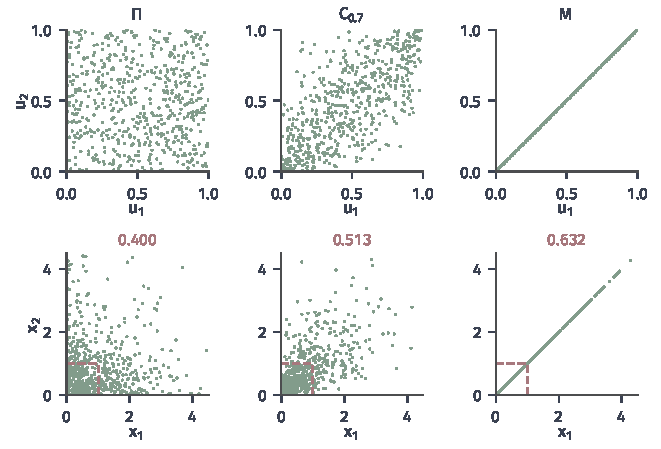
\includegraphics[width=112mm]{figures/07-probability/04-distribution-analysis/matplotlib/dfam-copula-samples/figure.pdf}
  \caption{同样的边缘，不同的依赖。上排：乘积Copula $\Pi$、$\rho=0.7$的高斯Copula、完全同向的$M$，各$600$个样本（绿，种子$716$）。下排：把上排每个点的两个坐标都用$u\mapsto-\ln(1-u)$变换，两个边缘都是$\operatorname{Exp}(1)$；红色虚线围出事件$\{X_1\leq1,X_2\leq1\}$，其概率依次约为$0.400$、$0.513$、$0.632$。}
  \label{fig:dfam-copula-samples}
\end{BookInlineFigure}

\paragraph{依赖的两个极端}
$M$与$W$分别是“完全同向”与“完全反向”的依赖，任何二元Copula都夹在它们之间。

\begin{lemma}[Fréchet–Hoeffding界]
\label{lem:dfam-frechet-bounds}
对任一二元Copula $C$与$u,v\in[0,1]$，
\begin{equation}
  W(u,v)\leq C(u,v)\leq M(u,v).
  \label{eq:dfam-frechet-bounds}
\end{equation}
\end{lemma}

\begin{proof}
设$(U_1,U_2)$的联合分布函数为$C$。事件$\{U_1\leq u,U_2\leq v\}$包含于$\{U_1\leq u\}$，也包含于$\{U_2\leq v\}$，所以$C(u,v)\leq u$且$C(u,v)\leq v$，即$C\leq M$。另一方面，由并集的概率公式，
\[
  C(u,v)=\mathbb{P}(U_1\leq u)+\mathbb{P}(U_2\leq v)-\mathbb{P}(U_1\leq u\text{或}U_2\leq v)\geq u+v-1 ,
\]
又$C(u,v)\geq0$，所以$C\geq W$。
\end{proof}

图~\ref{fig:dfam-copula-bounds}沿对角线比较几个Copula：$C(u,u)$是两个分量都不超过各自$u$分位数的概率。完全同向时它等于$u$，独立时是$u^{2}$，完全反向时在$u\leq1/2$以前一直为零。图中$u=0.632$处的四个值就是上面两台设备的四个概率。

\begin{BookInlineFigure}
  \centering
  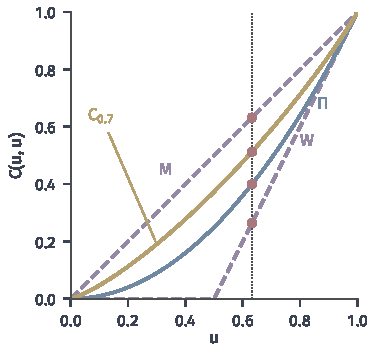
\includegraphics[width=64mm]{figures/07-probability/04-distribution-analysis/matplotlib/dfam-copula-bounds/figure.pdf}
  \caption{Copula在对角线上的取值$C(u,u)$。紫色虚线为上下界$M(u,u)=u$与$W(u,u)=\max(2u-1,0)$，蓝线为乘积Copula $u^{2}$，黄线为$\rho=0.7$的高斯Copula。红点标出$u=1-\mathrm{e}^{-1}\approx0.632$处的四个值$0.264,0.400,0.513,0.632$。}
  \label{fig:dfam-copula-bounds}
\end{BookInlineFigure}

\subsection{唯一性的范围}
\label{sec:dfam-copula-uniqueness}

现在反过来：给定$\bm{X}$的联合分布，能否找到它的Copula，找到的是否唯一？自然的想法是把每个分量用自己的分布函数送回$(0,1)$，令$U_i=F_i(X_i)$。这个想法在边缘连续时完全成立，在边缘有原子时会出问题。

\paragraph{连续边缘：概率积分变换}
先看一个分量。把$X$代入它自己的分布函数，得到$F(X)$，这个操作称为\term{概率积分变换}（probability integral transform）。

\begin{lemma}[概率积分变换]
\label{lem:dfam-pit}
设实值随机变量$X$的分布函数$F$连续。则$F(X)\sim\operatorname{Unif}(0,1)$，并且对每个$x$，事件$\{F(X)\leq F(x)\}$与$\{X\leq x\}$只差一个零概率事件。
\end{lemma}

\begin{proof}
记$Q$为$F$的分位数函数。对$u\in(0,1)$，由第~\ref{chap:random-variables}章的引理，$F(y)\geq u$当且仅当$y\geq Q(u)$，所以
\[
  \mathbb{P}\bigl(F(X)\geq u\bigr)=\mathbb{P}\bigl(X\geq Q(u)\bigr)=1-F\bigl(Q(u)-\bigr).
\]
另一方面，由同一引理有$F(Q(u))\geq u$；对$y<Q(u)$又有$F(y)<u$，令$y\uparrow Q(u)$得$F(Q(u)-)\leq u$。$F$连续，左极限等于函数值，两者合起来给出$F(Q(u))=u$。代入上式，
\[
  \mathbb{P}\bigl(F(X)\geq u\bigr)=1-u ,
\]
所以$F(X)$在$(0,1)$上均匀，又以概率$1$取值于$[0,1]$。

对第二个结论，$\{X\leq x\}\subseteq\{F(X)\leq F(x)\}$由单调性得到。差集是$\{X>x,\ F(X)=F(x)\}$，在其上$X$落在$F$取常值$F(x)$的区间里。记$b=\sup\{y:F(y)=F(x)\}$，这个事件包含于$\{x<X\leq b\}$（$b=+\infty$时为$\{X>x\}$），其概率是$F(b)-F(x)=0$（$b$有限时$F$连续，$F(b)=F(x)$；$b=+\infty$时$F(x)=1$）。
\end{proof}

\begin{proof}[Sklar定理第二部分的证明（边缘连续）]
设各$F_i$连续，令$U_i=F_i(X_i)$，$C$为$\bm{U}$的联合分布函数。由引理~\ref{lem:dfam-pit}，每个$U_i$均匀，$C$是Copula；且$\{U_i\leq F_i(x_i)\}$与$\{X_i\leq x_i\}$只差零概率事件，所以
\[
  C\bigl(F_1(x_1),\dots,F_d(x_d)\bigr)=\mathbb{P}(X_1\leq x_1,\dots,X_d\leq x_d)=F(x_1,\dots,x_d).
\]
唯一性：若$C'$也满足式~\eqref{eq:dfam-sklar}，则对每组$x_i$有$C'(F_1(x_1),\dots)=F(x_1,\dots)=C(F_1(x_1),\dots)$，所以$C'$与$C$在$\operatorname{Ran}F_1\times\cdots\times\operatorname{Ran}F_d$上相等。$F_i$连续时值域包含$(0,1)$，再由下面的引理~\ref{lem:dfam-copula-lipschitz}，$C$与$C'$都连续，于是在$[0,1]^{d}$上处处相等。
\end{proof}

\begin{lemma}[Copula的Lipschitz性]
\label{lem:dfam-copula-lipschitz}
对任一$d$元Copula $C$与$\bm{u},\bm{v}\in[0,1]^{d}$，
\begin{equation}
  \lvert C(\bm{u})-C(\bm{v})\rvert\leq\sum_{i=1}^{d}\lvert u_i-v_i\rvert .
  \label{eq:dfam-copula-lipschitz}
\end{equation}
\end{lemma}

\begin{proof}
设$\bm{U}$的联合分布函数为$C$。事件$\{\bm{U}\leq\bm{u}\}$与$\{\bm{U}\leq\bm{v}\}$的对称差中，至少有一个$i$使$U_i$落在$u_i$与$v_i$之间。由并集的概率不超过概率之和，
\[
  \lvert C(\bm{u})-C(\bm{v})\rvert\leq\sum_{i=1}^{d}\mathbb{P}\bigl(\min(u_i,v_i)<U_i\leq\max(u_i,v_i)\bigr)=\sum_{i=1}^{d}\lvert u_i-v_i\rvert ,
\]
最后一步用到$U_i$均匀。
\end{proof}

边缘连续时，唯一的Copula还有一个有用的性质。证明表明，这个Copula就是$(F_1(X_1),\dots,F_d(X_d))$的联合分布函数。设$g_1,\dots,g_d$都严格递增，$Y_i=g_i(X_i)$，其分布函数记为$G_i$。由$\{Y_i\leq g_i(x)\}=\{X_i\leq x\}$，
\[
  G_i\bigl(g_i(x)\bigr)=F_i(x),
\]
$G_i$也连续（$\mathbb{P}(Y_i=y)$不超过$X_i$取某个单点的概率，为零）。于是$G_i(Y_i)=F_i(X_i)$，$(Y_1,\dots,Y_d)$送回均匀刻度后得到的是同一个随机向量，Copula相同。分量各自作严格递增的重新刻度，Copula不变；依赖结构因此与单位、对数刻度这类选择无关，这正是“边缘以外的部分”应有的样子。

\paragraph{有原子时只在值域上唯一}
边缘有原子时，概率积分变换失效。取$X\sim\operatorname{Bern}(\tfrac12)$，$F(0)=\tfrac12$，$F(1)=1$，于是$F(X)$只取$\tfrac12$和$1$两个值，各有概率$\tfrac12$，根本不是均匀分布。图~\ref{fig:dfam-pit}(b)画出了这一点：质量在原子处不能被摊开；作为对照，(a)中连续的$\operatorname{Exp}(1)$经概率积分变换后确实均匀。

\begin{BookInlineFigure}
  \centering
  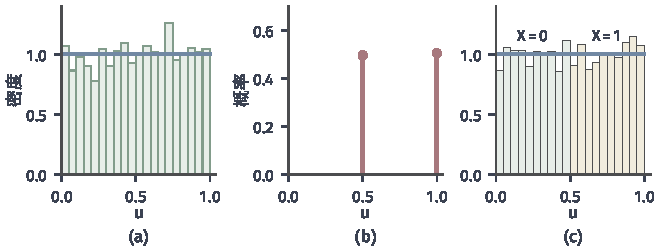
\includegraphics[width=112mm]{figures/07-probability/04-distribution-analysis/matplotlib/dfam-pit/figure.pdf}
  \caption{把分量送回均匀刻度，各$4000$个模拟值（种子$716$）。(a)$X\sim\operatorname{Exp}(1)$时$F(X)$的直方图（浅绿），蓝线是均匀密度$1$。(b)$X\sim\operatorname{Bern}(\frac12)$时$F(X)$只取$\frac12$与$1$（红色竖线，高度为概率）。(c)同一枚硬币的分布变换$U=F(X-)+V\Delta F(X)$：$X=0$的值摊在$(0,\frac12]$（浅绿），$X=1$的值摊在$(\frac12,1]$（浅黄），合起来是均匀分布。}
  \label{fig:dfam-pit}
\end{BookInlineFigure}

再看唯一性。设$X_1,X_2$是两枚独立的公平硬币。$\operatorname{Ran}F_i=\{0,\tfrac12,1\}$，式~\eqref{eq:dfam-sklar}只在这九个格点上约束$C$。$u$或$v$为$0$时任何Copula都取$0$，$u=1$时取$v$，$v=1$时取$u$，这些格点自动满足；真正的约束只有一个：
\[
  C(\tfrac12,\tfrac12)=\mathbb{P}(X_1=0,X_2=0)=\tfrac14 .
\]
乘积Copula满足它。$C'=\tfrac12M+\tfrac12W$也满足：两个Copula的凸组合仍是Copula（按权重混合两个均匀边缘的随机向量，边缘仍均匀），且
\[
  C'(\tfrac12,\tfrac12)=\tfrac12\cdot\tfrac12+\tfrac12\cdot0=\tfrac14 .
\]
可是在$(\tfrac14,\tfrac14)$处，$\Pi$取$\tfrac1{16}$，$C'$取$\tfrac12\cdot\tfrac14+0=\tfrac18$，两者不同。所以两枚独立硬币的联合分布既可以写成$\Pi(F_1,F_2)$，也可以写成$C'(F_1,F_2)$。

\begin{BookInlineFigure}
  \centering
  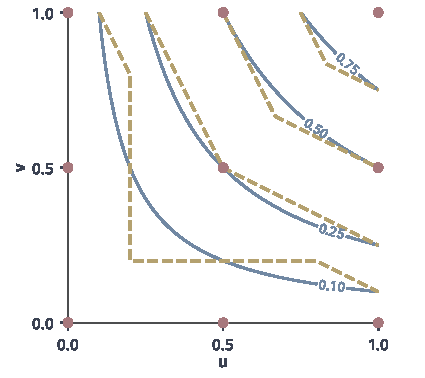
\includegraphics[width=72mm]{figures/07-probability/04-distribution-analysis/matplotlib/dfam-copula-atoms/figure.pdf}
  \caption{有原子时Copula只在值域格点上确定。两枚独立公平硬币，$\operatorname{Ran}F_1\times\operatorname{Ran}F_2$是九个格点（红点）。蓝色实线是乘积Copula $\Pi$的等值线，黄色虚线是$\frac12M+\frac12W$的等值线，层级为$0.1,0.25,0.5,0.75$；两族曲线在红点处取相同的值，在格点之间不同。}
  \label{fig:dfam-copula-atoms}
\end{BookInlineFigure}

图~\ref{fig:dfam-copula-atoms}画出这两个Copula的等值线：它们在九个红点上一致，在其他地方不同。这个例子说明，含原子时“从联合分布读出的Copula”并不唯一，不同的选择可能给人截然不同的依赖印象：$C'$看上去一半完全同向、一半完全反向，实际描述的却是两枚独立的硬币。连续情形的变换论证不能照搬，依据Copula谈论依赖时，必须先确认边缘是否连续。

\paragraph{有原子时的存在性}
唯一性失去了，存在性仍然成立。办法是在每个原子上用一个独立的均匀变量把质量摊开，这称为\term{分布变换}（distributional transform）。

\begin{lemma}[分布变换]
\label{lem:dfam-distributional-transform}
设$X$的分布函数为$F$，$V\sim\operatorname{Unif}(0,1)$与$X$独立，记$F(x-)$为左极限、$\Delta F(x)=F(x)-F(x-)$。令
\begin{equation}
  U=F(X-)+V\,\Delta F(X).
  \label{eq:dfam-distributional-transform}
\end{equation}
则$U\sim\operatorname{Unif}(0,1)$，并且对每个$x$，事件$\{U\leq F(x)\}$与$\{X\leq x\}$只差一个零概率事件。
\end{lemma}

\begin{proof}
固定$u\in(0,1)$，令$x_0=Q(u)$，则$F(x_0-)\leq u\leq F(x_0)$。由$V$与$X$独立，给定$X=y$时$U$在区间$[F(y-),F(y)]$上均匀（$\Delta F(y)=0$时退化为一点），所以
\[
  \mathbb{P}(U\leq u)=\mathbb{E}[g(X)],\qquad g(y)=\mathbb{P}\bigl(F(y-)+V\Delta F(y)\leq u\bigr).
\]
按$y$与$x_0$的位置分三种情形：
\begin{itemize}
  \item $y<x_0$：$F(y)\leq F(x_0-)\leq u$，$g(y)=1$，这部分贡献$\mathbb{P}(X<x_0)=F(x_0-)$。
  \item $y=x_0$：若$\Delta F(x_0)>0$，$g(x_0)=(u-F(x_0-))/\Delta F(x_0)$，贡献$\Delta F(x_0)\,g(x_0)=u-F(x_0-)$；若$\Delta F(x_0)=0$，则$F(x_0-)=u$，贡献为$0=u-F(x_0-)$。
  \item $y>x_0$：$F(y-)\geq F(x_0)\geq u$。$g(y)>0$只可能在$F(y-)=u$且$\Delta F(y)=0$时发生，这时$F(y)=F(x_0)$，$y$落在$F$取常值的区间里，这样的$y$整体的概率为零（与引理~\ref{lem:dfam-pit}的论证相同），贡献为$0$。
\end{itemize}
三部分相加，
\[
  \mathbb{P}(U\leq u)=F(x_0-)+\bigl(u-F(x_0-)\bigr)=u ,
\]
所以$U$均匀。

对第二个结论，$X\leq x$时$U\leq F(X)\leq F(x)$。$X>x$时$U\geq F(X-)\geq F(x)$，要使$U\leq F(x)$只能$U=F(x)=F(X-)$且$V\Delta F(X)=0$，即$V=0$，或者$\Delta F(X)=0$而$F(X)=F(x)$；前者概率为零，后者又是$X$落在$F$取常值的区间里，概率也为零。
\end{proof}

\begin{proof}[Sklar定理第二部分的证明（一般情形）]
取与$\bm{X}$独立的$V_1,\dots,V_d$，它们独立同分布于$\operatorname{Unif}(0,1)$，对每个分量按式~\eqref{eq:dfam-distributional-transform}作分布变换，得到$\bm{U}$，令$C$为它的联合分布函数。由引理~\ref{lem:dfam-distributional-transform}，$C$是Copula，且$\{U_i\leq F_i(x_i)\}$与$\{X_i\leq x_i\}$只差零概率事件，与连续情形一样得到式~\eqref{eq:dfam-sklar}。在$\operatorname{Ran}F_1\times\cdots\times\operatorname{Ran}F_d$上的唯一性，与连续情形的论证相同。
\end{proof}

分布变换在连续点上退化为$F(X)$，所以它是概率积分变换的推广。它得到的Copula依赖于为摊开原子而引入的独立变量$V_i$：图~\ref{fig:dfam-pit}(c)中，硬币的两个原子各被摊成长为$\tfrac12$的一段，两枚独立硬币配独立的$V_1,V_2$，得到的正是乘积Copula；若让$V_1=V_2$，就得到另一个同样合法的Copula。这再次说明含原子时Copula是联合分布的一种表示，而不是由它唯一决定的量。


\section{指数族}
\label{sec:dfam-exponential}

把Bernoulli、Poisson和高斯的概率公式取对数，会看到同一个结构。Bernoulli分布的对数质量是$x\ln\frac{p}{1-p}+\ln(1-p)$，Poisson分布是$x\ln\lambda-\lambda-\ln x!$，高斯分布是$x$与$x^{2}$的线性组合再加常数。三者都是“若干个统计量的线性组合，加上只依赖参数的归一化项，再加上只依赖$x$的项”。改变参数，就是改变给每个统计量的指数权重。

这一节先把这种形式写准，区分哪些对象固定、哪些随参数变化；再确定参数能取哪些值；然后看归一化项的导数怎样给出矩；最后把指数权重与它产生的均值对应起来。

\subsection{指数形式}
\label{sec:dfam-exponential-form}

\begin{definition}[指数族]
\label{def:dfam-exponential-family}
设$\nu$是$\mathcal{X}$上的$\sigma$有限测度，$h:\mathcal{X}\to[0,\infty)$与$\bm{T}:\mathcal{X}\to\mathbb{R}^{k}$可测，$\nu(\{h>0\})>0$。对使
\begin{equation}
  Z(\bm{\theta})=\int_{\mathcal{X}}h(x)\,\mathrm{e}^{\langle\bm{\theta},\bm{T}(x)\rangle}\,\nu(\mathrm{d}x)<\infty
  \label{eq:dfam-partition}
\end{equation}
的$\bm{\theta}\in\mathbb{R}^{k}$，令$A(\bm{\theta})=\ln Z(\bm{\theta})$，并以
\begin{equation}
  p_{\bm{\theta}}(x)=h(x)\exp\bigl(\langle\bm{\theta},\bm{T}(x)\rangle-A(\bm{\theta})\bigr)
  \label{eq:dfam-exponential-family}
\end{equation}
为相对$\nu$的密度定义$P_{\bm{\theta}}$。这样得到的分布族称为\term{指数族}（exponential family）。$\bm{T}$称为\term{自然统计量}（natural statistic），$\bm{\theta}$称为\term{自然参数}（natural parameter），$Z$与$A$分别称为\term{配分函数}（partition function）与\term{对数配分函数}（log-partition function）。
\end{definition}

式~\eqref{eq:dfam-exponential-family}中有三样东西是事先固定的：参考测度$\nu$、函数$h$和统计量$\bm{T}$。$h$与$\nu$只以乘积$h(x)\nu(\mathrm{d}x)$的形式出现，这个乘积称为\term{基准测度}（base measure），它决定哪些$x$可能出现，以及在不加任何指数权重时质量怎样分布。随参数变化的只有$\bm{\theta}$；$A(\bm{\theta})$不是另一个可以自由选择的量，它由归一化唯一确定，保证$p_{\bm{\theta}}$积分为$1$。

由式~\eqref{eq:dfam-exponential-family}，$p_{\bm{\theta}}(x)>0$当且仅当$h(x)>0$。所以指数族的所有成员有共同的支撑$\{h>0\}$，参数只改变支撑上质量的相对多少，不能把质量挪到$h$为零的地方。$\operatorname{Unif}(0,\theta)$的支撑随$\theta$变化，它就不能写成任何指数族。

\paragraph{三个分布的指数形式}
Bernoulli分布取$\nu$为$\{0,1\}$上的计数测度，
\[
  p^{x}(1-p)^{1-x}=\exp\Bigl(x\ln\frac{p}{1-p}+\ln(1-p)\Bigr).
\]
对照式~\eqref{eq:dfam-exponential-family}，$h=1$，$T(x)=x$，自然参数$\theta=\ln\frac{p}{1-p}$，即$p=\mathrm{e}^{\theta}/(1+\mathrm{e}^{\theta})$，再由$-A(\theta)=\ln(1-p)$得
\[
  A(\theta)=\ln(1+\mathrm{e}^{\theta}).
\]

Poisson分布取$\nu$为$\{0,1,2,\dots\}$上的计数测度，
\[
  \mathrm{e}^{-\lambda}\frac{\lambda^{x}}{x!}=\frac{1}{x!}\exp(x\ln\lambda-\lambda),
\]
所以$h(x)=1/x!$，$T(x)=x$，$\theta=\ln\lambda$，$A(\theta)=\mathrm{e}^{\theta}$。

高斯分布$\mathcal{N}(m,s^{2})$取$\nu$为Lebesgue测度，把指数中的平方展开：
\[
  \frac{1}{\sqrt{2\pi s^{2}}}\mathrm{e}^{-\frac{(x-m)^{2}}{2s^{2}}}=\frac{1}{\sqrt{2\pi}}\exp\Bigl(\frac{m}{s^{2}}x-\frac{1}{2s^{2}}x^{2}-\frac{m^{2}}{2s^{2}}-\ln s\Bigr).
\]
于是$h=1/\sqrt{2\pi}$，$\bm{T}(x)=(x,x^{2})$，自然参数是
\begin{equation}
  \bm{\theta}=(\theta_1,\theta_2)=\Bigl(\frac{m}{s^{2}},\ -\frac{1}{2s^{2}}\Bigr).
  \label{eq:dfam-gaussian-natural}
\end{equation}
反解得$s^{2}=-1/(2\theta_2)$，$m=-\theta_1/(2\theta_2)$，代入$\frac{m^{2}}{2s^{2}}+\ln s$，得到
\begin{equation}
  A(\bm{\theta})=-\frac{\theta_1^{2}}{4\theta_2}-\frac12\ln(-2\theta_2).
  \label{eq:dfam-gaussian-log-partition}
\end{equation}

\paragraph{同一个分布的不同写法}
指数形式不是唯一的。把高斯的统计量换成$\bm{T}'(x)=(x,-x^{2}/2)$，自然参数就变成$(m/s^{2},\ 1/s^{2})$；常数$1/\sqrt{2\pi}$也可以从$h$移进$A$。一般地，统计量作可逆线性变换$\bm{T}'=\bm{L}\bm{T}$，自然参数就作相应的变换$\bm{\theta}'=\bm{L}^{-\top}\bm{\theta}$，于是
\[
  \langle\bm{\theta}',\bm{T}'\rangle=\bm{\theta}^{\top}\bm{L}^{-1}\bm{L}\bm{T}=\langle\bm{\theta},\bm{T}\rangle ,
\]
指数不变，分布族也不变。

所以“自然参数”是相对于选定的$\bm{T}$与$h\nu$而言的，不能把密度公式里出现的任意参数都叫作自然参数。高斯族的均值$m$在式~\eqref{eq:dfam-gaussian-natural}中与$s^{2}$纠缠在一起，又出现在$A$里，它不是这组表示下的自然参数。但若只看方差固定为$1$的子族$\{\mathcal{N}(m,1)\}$，取$h=\varphi$、$T(x)=x$，则
\[
  \varphi(x-m)=\varphi(x)\exp\bigl(mx-\tfrac12m^{2}\bigr),
\]
$m$恰好是自然参数，$A(m)=m^{2}/2$。同一个数字是否是自然参数，取决于整个表示。

写法还可能带来冗余。Bernoulli分布也可以写成
\[
  p^{x}(1-p)^{1-x}=\exp\bigl(\theta_0\mathbf{1}_{\{x=0\}}+\theta_1\mathbf{1}_{\{x=1\}}\bigr),\qquad(\theta_0,\theta_1)=(\ln(1-p),\ln p).
\]
两个统计量之和恒为$1$，把$(\theta_0,\theta_1)$同时加上同一个常数，归一化后分布不变。这种冗余与第~\ref{sec:dfam-identifiability}节的重复参数是同一回事，后面两小节会精确地描述它。

\subsection{自然参数域}
\label{sec:dfam-natural-domain}

式~\eqref{eq:dfam-exponential-family}只在$Z(\bm{\theta})$有限且为正时才定义了概率分布。被积函数在$\{h>0\}$上为正，而$\nu(\{h>0\})>0$，所以$Z(\bm{\theta})>0$总成立；问题只在于是否有限。

\begin{definition}[自然参数域]
\label{def:dfam-natural-domain}
集合
\begin{equation}
  \Theta=\{\bm{\theta}\in\mathbb{R}^{k}:Z(\bm{\theta})<\infty\}
  \label{eq:dfam-natural-domain}
\end{equation}
称为指数族的\term{自然参数域}（natural parameter space）。若$\Theta$是$\mathbb{R}^{k}$中的开集，称这个指数族是\term{正则指数族}（regular exponential family）。
\end{definition}

$\Theta$以外的$\bm{\theta}$给出的表达式$h\,\mathrm{e}^{\langle\bm{\theta},\bm{T}\rangle}$不能归一化，它只是一个形式表达式，不是概率分布。例如在$(0,\infty)$上取$h=1$、$T(x)=x$，$\int_0^\infty\mathrm{e}^{\theta x}\,\mathrm{d}x$在$\theta<0$时等于$-1/\theta$，在$\theta\geq0$时发散。所以$\Theta=(-\infty,0)$，$\theta=-\lambda$对应$\operatorname{Exp}(\lambda)$，$A(\theta)=-\ln(-\theta)$。

\begin{lemma}[自然参数域的凸性]
\label{lem:dfam-domain-convex}
$\Theta$是凸集，$A$是$\Theta$上的凸函数。
\end{lemma}

\begin{proof}
设$\bm{\theta},\bm{\theta}'\in\Theta$，$0<\lambda<1$。被积函数可以拆成两个幂的乘积：
\[
  \mathrm{e}^{\langle\lambda\bm{\theta}+(1-\lambda)\bm{\theta}',\bm{T}\rangle}=\bigl(\mathrm{e}^{\langle\bm{\theta},\bm{T}\rangle}\bigr)^{\lambda}\bigl(\mathrm{e}^{\langle\bm{\theta}',\bm{T}\rangle}\bigr)^{1-\lambda}.
\]
对测度$h\nu$用指数为$1/\lambda$与$1/(1-\lambda)$的Hölder不等式（见\BookChapterRef{chap:function-normed-spaces}{卷四第11章“赋范空间”}），
\[
  Z\bigl(\lambda\bm{\theta}+(1-\lambda)\bm{\theta}'\bigr)\leq Z(\bm{\theta})^{\lambda}Z(\bm{\theta}')^{1-\lambda}<\infty .
\]
所以$\lambda\bm{\theta}+(1-\lambda)\bm{\theta}'\in\Theta$。两边取对数，得到
\[
  A\bigl(\lambda\bm{\theta}+(1-\lambda)\bm{\theta}'\bigr)\leq\lambda A(\bm{\theta})+(1-\lambda)A(\bm{\theta}') .
\]
\end{proof}

\paragraph{几个参数域}
Bernoulli与Poisson的配分和对任何$\theta$都有限，$\Theta=\mathbb{R}$。高斯族的配分积分是
\[
  Z(\bm{\theta})=\frac{1}{\sqrt{2\pi}}\int_{-\infty}^{\infty}\mathrm{e}^{\theta_1x+\theta_2x^{2}}\,\mathrm{d}x ,
\]
它在$\theta_2<0$时有限；$\theta_2=0$时被积函数是$\mathrm{e}^{\theta_1x}$，在某一侧不衰减；$\theta_2>0$时在两侧都发散。所以$\Theta=\{(\theta_1,\theta_2):\theta_2<0\}$是开半平面，高斯族是正则的。

自然参数域不一定是开的。在$(0,\infty)$上取$h(x)=(1+x)^{-2}$、$T(x)=x$，
\[
  Z(\theta)=\int_0^\infty\frac{\mathrm{e}^{\theta x}}{(1+x)^{2}}\,\mathrm{d}x .
\]
$\theta>0$时被积函数趋于无穷，积分发散；$\theta\leq0$时被积函数不超过$(1+x)^{-2}$，积分有限，且$Z(0)=1$。所以$\Theta=(-\infty,0]$，边界点$0$属于参数域，它对应的分布就是密度$(1+x)^{-2}$。这个分布的均值是$\int_0^\infty x(1+x)^{-2}\,\mathrm{d}x=\infty$。

图~\ref{fig:dfam-natural-domain}比较这两个一维的例子。指数分布族的$A(\theta)$在$\theta\uparrow0$时趋于无穷，参数域在$0$处断开；第二个族的$A(\theta)$在$0$处取有限值$0$，但均值$\mathbb{E}_\theta[X]$在$\theta\uparrow0$时趋于无穷，曲线在边界处变得竖直。边界点属于参数域，并不意味着那里的分布与内部一样好用：它的均值已经不存在了，下一小节的导数公式在那里不成立。

\begin{BookInlineFigure}
  \centering
  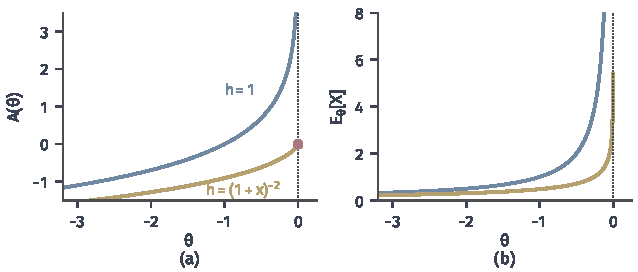
\includegraphics[width=108mm]{figures/07-probability/04-distribution-analysis/matplotlib/dfam-natural-domain/figure.pdf}
  \caption{两个一维指数族的自然参数域，$T(x)=x$，$x>0$。蓝：$h=1$（指数分布族），$\Theta=(-\infty,0)$；黄：$h(x)=(1+x)^{-2}$，$\Theta=(-\infty,0]$，红点是属于参数域的边界点$\theta=0$。(a)对数配分函数$A(\theta)$。(b)均值$\mathbb{E}_\theta[X]$，两者在$\theta\uparrow0$时都趋于无穷。黄线由数值积分得到。}
  \label{fig:dfam-natural-domain}
\end{BookInlineFigure}

\paragraph{退化的极限}
参数趋于无穷时，分布可能趋于族外的分布。在$\{0,1,2\}$上取计数测度、$h=1$、$T(x)=x$，得到一个单参数指数族
\begin{equation}
  p_\theta(x)=\frac{\mathrm{e}^{\theta x}}{1+\mathrm{e}^{\theta}+\mathrm{e}^{2\theta}},\qquad x=0,1,2,\quad\theta\in\mathbb{R}.
  \label{eq:dfam-tilt}
\end{equation}
它从均匀表出发，按$\mathrm{e}^{\theta x}$给较大的点数加权：$\theta=0$时是均匀表，$\theta=\ln2$时权重为$1,2,4$，
\[
  p_{\ln2}=\bigl(\tfrac17,\ \tfrac27,\ \tfrac47\bigr).
\]
$\theta\to+\infty$时，分子分母同除以$\mathrm{e}^{2\theta}$，$p_\theta(2)\to1$，分布趋于点质量$\delta_2$；$\theta\to-\infty$时趋于$\delta_0$。

但$\delta_2$不等于任何$p_\theta$，因为每个$p_\theta$在三个点上都为正。图~\ref{fig:dfam-tilt-simplex}把这个族画在第~\ref{sec:dfam-candidates}节的三角形中：它是穿过内部的一条曲线，两端无限接近顶点而不到达。族的闭包含有边界上的分布，而这些分布不能用有限的自然参数表示。

\begin{BookInlineFigure}
  \centering
  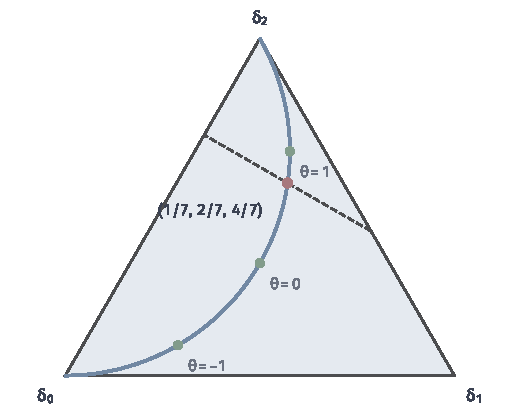
\includegraphics[width=88mm]{figures/07-probability/04-distribution-analysis/matplotlib/dfam-tilt-simplex/figure.pdf}
  \caption{式~\eqref{eq:dfam-tilt}的单参数指数族在三角形$\Delta_2$中的轨迹（蓝线），$\theta$从$-6$到$6$。绿点依次是$\theta=-1,0,1$，红点是$\theta=\ln2$对应的$(\frac17,\frac27,\frac47)$；曲线两端趋于顶点$\delta_0$与$\delta_2$，但不到达。深灰虚线是满足$\mathbb{E}_P[X]=\frac{10}{7}$的全部概率表，它与曲线只交于红点。}
  \label{fig:dfam-tilt-simplex}
\end{BookInlineFigure}

\subsection{配分函数的导数}
\label{sec:dfam-partition-derivatives}

对数配分函数原本只是为归一化而设，但它把整个族的矩都存了起来。对式~\eqref{eq:dfam-partition}关于$\theta_j$求导，形式上会在积分号内落下一个因子$T_j(x)$，这正是$T_j$的期望。下面的定理说明，在参数域内部这个形式计算是合法的。

\begin{theorem}[对数配分函数的导数]
\label{thm:dfam-log-partition-derivatives}
设$\bm{\theta}$是$\Theta$的内点。则在$P_{\bm{\theta}}$下$\bm{T}$的各分量有任意阶矩，$A$在$\bm{\theta}$处二阶可微，且
\begin{equation}
  \nabla A(\bm{\theta})=\mathbb{E}_{\bm{\theta}}[\bm{T}],\qquad\nabla^{2}A(\bm{\theta})=\operatorname{Cov}_{\bm{\theta}}(\bm{T}).
  \label{eq:dfam-log-partition-derivatives}
\end{equation}
\end{theorem}

\begin{proof}
取$\varepsilon>0$，使立方体$K=\bm{\theta}+[-2\varepsilon,2\varepsilon]^{k}$含于$\Theta$。函数$\bm{\eta}\mapsto\mathrm{e}^{\langle\bm{\eta},\bm{T}(x)\rangle}$是凸的，它在立方体$K$上的最大值在某个顶点处取到，所以对$\bm{\eta}\in K$，
\[
  \mathrm{e}^{\langle\bm{\eta},\bm{T}(x)\rangle}\leq G(x)=\sum_{\bm{v}}\mathrm{e}^{\langle\bm{v},\bm{T}(x)\rangle},
\]
其中$\bm{v}$取遍$K$的$2^{k}$个顶点。每个顶点都在$\Theta$中，所以$G$对$h\nu$可积。

再把统计量的多项式因子吸收进指数。由$\mathrm{e}^{s}\geq s$与$\mathrm{e}^{s}\geq s^{2}/2$（$s\geq0$），对实数$t$有
\[
  \lvert t\rvert\leq\frac{\mathrm{e}^{\varepsilon t}+\mathrm{e}^{-\varepsilon t}}{\varepsilon},\qquad t^{2}\leq\frac{2(\mathrm{e}^{\varepsilon t}+\mathrm{e}^{-\varepsilon t})}{\varepsilon^{2}} .
\]
设$\bm{\theta}'\in\bm{\theta}+[-\varepsilon,\varepsilon]^{k}$，则$\bm{\theta}'\pm\varepsilon\bm{e}_j\in K$。取$t=T_j(x)$，第二个不等式给出
\[
  T_j(x)^{2}\,\mathrm{e}^{\langle\bm{\theta}',\bm{T}(x)\rangle}\leq\frac{2}{\varepsilon^{2}}\bigl(\mathrm{e}^{\langle\bm{\theta}'+\varepsilon\bm{e}_j,\bm{T}\rangle}+\mathrm{e}^{\langle\bm{\theta}'-\varepsilon\bm{e}_j,\bm{T}\rangle}\bigr)\leq\frac{4}{\varepsilon^{2}}G(x).
\]
用第一个不等式同样得到
\[
  \lvert T_j\rvert\,\mathrm{e}^{\langle\bm{\theta}',\bm{T}\rangle}\leq\frac{2}{\varepsilon}G ,
\]
而由$\lvert T_iT_j\rvert\leq(T_i^{2}+T_j^{2})/2$，交叉项也被$4G/\varepsilon^{2}$控制。对更高的$r$次幂，由$\mathrm{e}^{s}\geq s^{r}/r!$（$s\geq0$）同样把$\lvert T_j\rvert^{r}$吸收进指数，得到任意阶矩有限。

有了与$\bm{\theta}'$无关的可积控制函数，由中值定理与控制收敛定理，可以在积分号下对$Z$求一阶和二阶偏导数（见\BookChapterRef{chap:integration}{卷四第6章“积分”}）：
\[
  \partial_jZ(\bm{\theta})=\int T_j\,h\,\mathrm{e}^{\langle\bm{\theta},\bm{T}\rangle}\,\mathrm{d}\nu,\qquad\partial_i\partial_jZ(\bm{\theta})=\int T_iT_j\,h\,\mathrm{e}^{\langle\bm{\theta},\bm{T}\rangle}\,\mathrm{d}\nu ,
\]
并且这些偏导数在$\bm{\theta}$附近连续。

除以$Z(\bm{\theta})$，就是$P_{\bm{\theta}}$下的期望：
\[
  \frac{\partial_jZ}{Z}=\mathbb{E}_{\bm{\theta}}[T_j],\qquad\frac{\partial_i\partial_jZ}{Z}=\mathbb{E}_{\bm{\theta}}[T_iT_j].
\]
由$A=\ln Z$，一阶偏导数是
\[
  \partial_jA=\frac{\partial_jZ}{Z}=\mathbb{E}_{\bm{\theta}}[T_j].
\]
再求一次导，
\[
  \partial_i\partial_jA=\frac{\partial_i\partial_jZ}{Z}-\frac{\partial_iZ\,\partial_jZ}{Z^{2}}=\mathbb{E}_{\bm{\theta}}[T_iT_j]-\mathbb{E}_{\bm{\theta}}[T_i]\,\mathbb{E}_{\bm{\theta}}[T_j].
\]
这就是$\operatorname{Cov}_{\bm{\theta}}(T_i,T_j)$。
\end{proof}

定理只对内点成立。上一小节的边界点$\theta=0$处，$\mathbb{E}_0[X]=\infty$，一阶导数公式已经失去意义。

\paragraph{例子中的导数}
Bernoulli族$A(\theta)=\ln(1+\mathrm{e}^{\theta})$，求导得
\[
  A'(\theta)=\frac{\mathrm{e}^{\theta}}{1+\mathrm{e}^{\theta}}=p,\qquad A''(\theta)=p(1-p),
\]
正是$\operatorname{Bern}(p)$的均值与方差。Poisson族$A(\theta)=\mathrm{e}^{\theta}=\lambda$，一阶、二阶导数都等于$\lambda$，均值与方差相等。

高斯族对式~\eqref{eq:dfam-gaussian-log-partition}求偏导，再用$m=-\theta_1/(2\theta_2)$与$s^{2}=-1/(2\theta_2)$换回去，
\[
  \frac{\partial A}{\partial\theta_1}=-\frac{\theta_1}{2\theta_2}=m,\qquad\frac{\partial A}{\partial\theta_2}=\frac{\theta_1^{2}}{4\theta_2^{2}}-\frac{1}{2\theta_2}=m^{2}+s^{2}.
\]
这正是$\mathbb{E}[X]$与$\mathbb{E}[X^{2}]$，与$\bm{T}=(x,x^{2})$对应。

对式~\eqref{eq:dfam-tilt}的族，对数配分函数是
\[
  A(\theta)=\ln\bigl(1+\mathrm{e}^{\theta}+\mathrm{e}^{2\theta}\bigr).
\]
在$\theta=\ln2$处，$\mathrm{e}^{\theta}=2$，
\[
  A(\ln2)=\ln7,\qquad A'(\ln2)=\frac{2+2\cdot4}{7}=\frac{10}{7}.
\]
再算二阶矩$\mathbb{E}[X^{2}]=(2+4\cdot4)/7=18/7$，于是
\[
  A''(\ln2)=\frac{18}{7}-\Bigl(\frac{10}{7}\Bigr)^{2}=\frac{26}{49}\approx0.531 .
\]
图~\ref{fig:dfam-log-partition}(a)中，红点处切线的斜率$10/7$就是这个分布的均值；(b)画出均值$A'(\theta)$与方差$A''(\theta)$随$\theta$的变化：均值从$0$单调升到$2$，方差在均值经过$1$时最大，在两端趋于零。

\begin{BookInlineFigure}
  \centering
  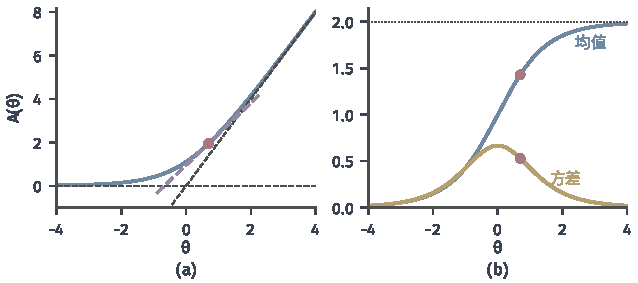
\includegraphics[width=108mm]{figures/07-probability/04-distribution-analysis/matplotlib/dfam-log-partition/figure.pdf}
  \caption{式~\eqref{eq:dfam-tilt}的对数配分函数。(a)$A(\theta)=\ln(1+\mathrm{e}^{\theta}+\mathrm{e}^{2\theta})$（蓝），红点$\theta=\ln2$处的切线（紫色虚线）斜率为$10/7$；两条深灰虚线是渐近线$y=0$与$y=2\theta$。(b)均值$A'(\theta)$（蓝）与方差$A''(\theta)$（黄），红点为$(\ln2,10/7)$与$(\ln2,26/49)$。}
  \label{fig:dfam-log-partition}
\end{BookInlineFigure}

\paragraph{累积量}
导数还能继续求下去。对$\bm{\theta}\in\Theta$与使$\bm{\theta}+\bm{t}\in\Theta$的$\bm{t}$，
\begin{equation}
  \ln\mathbb{E}_{\bm{\theta}}\bigl[\mathrm{e}^{\langle\bm{t},\bm{T}\rangle}\bigr]=\ln\frac{Z(\bm{\theta}+\bm{t})}{Z(\bm{\theta})}=A(\bm{\theta}+\bm{t})-A(\bm{\theta}).
  \label{eq:dfam-cumulant}
\end{equation}
左边是$\bm{T}$的矩母函数的对数，称为\term{累积量生成函数}（cumulant generating function）。式~\eqref{eq:dfam-cumulant}说明，在一个内点处，它就是把$A$平移到原点。$\bm{T}$在$P_{\bm{\theta}}$下的全部高阶矩信息，都由$A$在$\bm{\theta}$附近的形状给出。

\paragraph{凸性与仿射冗余}
由式~\eqref{eq:dfam-log-partition-derivatives}，对任意$\bm{a}\in\mathbb{R}^{k}$，
\[
  \bm{a}^{\top}\nabla^{2}A(\bm{\theta})\,\bm{a}=\operatorname{Var}_{\bm{\theta}}\bigl(\langle\bm{a},\bm{T}\rangle\bigr)\geq0 ,
\]
Hessian半正定，与引理~\ref{lem:dfam-domain-convex}的凸性相符。等号成立当且仅当$\langle\bm{a},\bm{T}\rangle$在$P_{\bm{\theta}}$下几乎必然为常数。

$P_{\bm{\theta}}$的密度在$\{h>0\}$上为正，所以$P_{\bm{\theta}}$与基准测度$h\nu$有相同的零测集，“$P_{\bm{\theta}}$下几乎必然”就是“$h\nu$下几乎处处”，与$\bm{\theta}$无关。于是Hessian在某个内点退化，当且仅当存在$\bm{a}\neq\bm{0}$与常数$c$，使
\begin{equation}
  \langle\bm{a},\bm{T}(x)\rangle=c\qquad\text{对}h\nu\text{几乎所有}x ,
  \label{eq:dfam-affine-redundancy}
\end{equation}
而这时它在所有内点处同时退化。式~\eqref{eq:dfam-affine-redundancy}说的是统计量之间有仿射关系，有一个分量是多余的。

第~\ref{sec:dfam-exponential-form}节Bernoulli的冗余写法正是如此：两个示性统计量满足$T_0+T_1=1$，取$\bm{a}=(1,1)$、$c=1$。这时
\[
  A(\bm{\theta})=\ln(\mathrm{e}^{\theta_0}+\mathrm{e}^{\theta_1}),\qquad A\bigl(\bm{\theta}+c'(1,1)\bigr)=A(\bm{\theta})+c',
\]
$A$沿$(1,1)$方向是线性的，不是严格凸的；而分布只依赖$\theta_1-\theta_0=\ln\frac{p}{1-p}$，沿这个方向完全不变。图~\ref{fig:dfam-overcomplete}画出这一点。

\begin{BookInlineFigure}
  \centering
  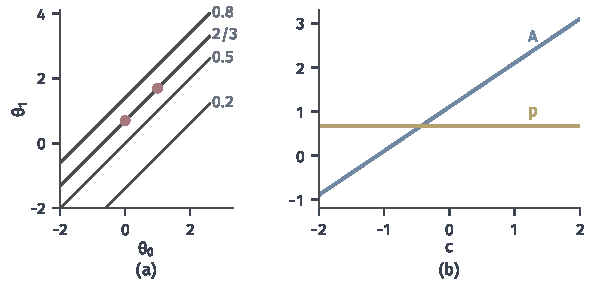
\includegraphics[width=100mm]{figures/07-probability/04-distribution-analysis/matplotlib/dfam-overcomplete/figure.pdf}
  \caption{Bernoulli族的冗余表示$\bm{T}=(\mathbf{1}_{\{x=0\}},\mathbf{1}_{\{x=1\}})$。(a)$(\theta_0,\theta_1)$平面中，分布相同的参数构成平行于$(1,1)$的直线（深灰），标注为对应的$p$；红点$(0,\ln2)$与$(1,1+\ln2)$都给出$p=\frac23$。(b)沿红点所在直线$\bm{\theta}=(0,\ln2)+c(1,1)$，$A$随$c$线性增长（蓝），而$p$保持$\frac23$（黄）。}
  \label{fig:dfam-overcomplete}
\end{BookInlineFigure}

\subsection{自然参数与均值参数}
\label{sec:dfam-natural-mean}

上一小节表明，Hessian退化与参数冗余是同一个现象。把统计量中多余的分量去掉，参数就不再冗余，而$\nabla A$给出的均值成为另一套可以替代自然参数的坐标。

\begin{definition}[最小表示与均值参数]
\label{def:dfam-minimal}
若不存在$\bm{a}\neq\bm{0}$与常数$c$使式~\eqref{eq:dfam-affine-redundancy}成立，则称指数族的这个表示是\term{最小表示}（minimal representation）。对$\bm{\theta}\in\Theta$，若$\mathbb{E}_{\bm{\theta}}[\bm{T}]$存在，称
\begin{equation}
  \bm{m}(\bm{\theta})=\mathbb{E}_{\bm{\theta}}[\bm{T}]
  \label{eq:dfam-mean-parameter}
\end{equation}
为$P_{\bm{\theta}}$的\term{均值参数}（mean parameter），$\bm{\theta}\mapsto\bm{m}(\bm{\theta})$称为\term{均值映射}（mean map）。
\end{definition}

在正则族中，每个$\bm{\theta}$都是内点，由定理~\ref{thm:dfam-log-partition-derivatives}，均值映射就是$\nabla A$。

\begin{theorem}[自然参数与均值参数的对应]
\label{thm:dfam-natural-mean}
设指数族采用最小表示。
\begin{enumerate}
  \item 参数化$\bm{\theta}\mapsto P_{\bm{\theta}}$在$\Theta$上可辨识。反之，若表示不是最小的，则参数化不可辨识。
  \item 若族还是正则的，则均值映射$\bm{m}=\nabla A$在$\Theta$上是单射，其Jacobian矩阵$\nabla^{2}A(\bm{\theta})$正定；像集$\mathcal{M}^{\circ}=\nabla A(\Theta)$是开集，逆映射$\mathcal{M}^{\circ}\to\Theta$连续可微。
  \item 在第二部分的条件下，若$\bm{a}\neq\bm{0}$且$\langle\bm{a},\bm{T}\rangle\leq c$对$h\nu$几乎所有$x$成立，则对每个$\bm{m}\in\mathcal{M}^{\circ}$有$\langle\bm{a},\bm{m}\rangle<c$。
\end{enumerate}
\end{theorem}

\begin{proof}
第一部分。设$P_{\bm{\theta}}=P_{\bm{\theta}'}$，则两个密度在$h\nu$下几乎处处相等。在$\{h>0\}$上取对数，得到
\[
  \langle\bm{\theta}-\bm{\theta}',\bm{T}(x)\rangle=A(\bm{\theta})-A(\bm{\theta}')\qquad\text{对}h\nu\text{几乎所有}x .
\]
这是形如式~\eqref{eq:dfam-affine-redundancy}的关系，$\bm{a}=\bm{\theta}-\bm{\theta}'$。最小表示排除了$\bm{a}\neq\bm{0}$，所以$\bm{\theta}=\bm{\theta}'$。

反之，若式~\eqref{eq:dfam-affine-redundancy}对某个$\bm{a}\neq\bm{0}$成立，取$\bm{\theta}\in\Theta$与$t\neq0$。在$h\nu$下几乎处处有
\[
  \mathrm{e}^{\langle\bm{\theta}+t\bm{a},\bm{T}\rangle}=\mathrm{e}^{tc}\,\mathrm{e}^{\langle\bm{\theta},\bm{T}\rangle},
\]
两边积分，
\[
  Z(\bm{\theta}+t\bm{a})=\mathrm{e}^{tc}Z(\bm{\theta})<\infty ,
\]
所以$\bm{\theta}+t\bm{a}\in\Theta$。两个密度中的因子$\mathrm{e}^{tc}$被归一化抵消，$P_{\bm{\theta}+t\bm{a}}=P_{\bm{\theta}}$，参数化不可辨识。

第二部分。由上一小节，最小表示下$\nabla^{2}A(\bm{\theta})$对每个$\bm{\theta}\in\Theta$正定。设$\bm{\theta}\neq\bm{\theta}'$，令$g(t)=A(\bm{\theta}'+t(\bm{\theta}-\bm{\theta}'))$，$t\in[0,1]$。$\Theta$凸，线段在$\Theta$内，
\[
  g''(t)=(\bm{\theta}-\bm{\theta}')^{\top}\nabla^{2}A\,(\bm{\theta}-\bm{\theta}')>0 ,
\]
所以$g'$严格递增，$g'(1)>g'(0)$，即
\[
  \bigl\langle\nabla A(\bm{\theta})-\nabla A(\bm{\theta}'),\ \bm{\theta}-\bm{\theta}'\bigr\rangle>0 .
\]
这说明$\nabla A(\bm{\theta})\neq\nabla A(\bm{\theta}')$，均值映射是单射。定理~\ref{thm:dfam-log-partition-derivatives}的证明给出$\nabla A$连续可微，Jacobian矩阵$\nabla^{2}A$正定因而可逆。由反函数定理（见\BookChapterRef{chap:implicit-inverse-functions}{卷二第22章“隐函数与反函数”}），$\nabla A$把每个点的一个邻域连续可微地一一映到一个开集上，于是像集$\mathcal{M}^{\circ}$是开集；结合全局单射，这些局部逆拼成一个连续可微的全局逆。

第三部分。设$\bm{m}=\nabla A(\bm{\theta})$且$\langle\bm{a},\bm{m}\rangle=c$。则$c-\langle\bm{a},\bm{T}\rangle$在$P_{\bm{\theta}}$下几乎必然非负，期望为零，所以几乎必然为零，也就是在$h\nu$下几乎处处有$\langle\bm{a},\bm{T}\rangle=c$，与最小表示矛盾。而$\langle\bm{a},\bm{m}\rangle\leq c$由期望的保序得到，所以严格不等式成立。
\end{proof}

第三部分说的是：统计量的取值被一个半空间$\{\langle\bm{a},\bm{t}\rangle\leq c\}$围住时，族中任何分布的均值都严格落在半空间内部，碰不到边界。边界上的均值只能由把全部质量放在超平面$\{\langle\bm{a},\bm{t}\rangle=c\}$上的分布实现，而指数族的成员都与基准测度有相同的零测集，做不到这一点。

\paragraph{三个例子}
Bernoulli族是最小表示，均值参数就是$p$。所有$\{0,1\}$上分布的均值组成$[0,1]$，均值映射的像却只是$(0,1)$：端点$0$与$1$是$\delta_0$与$\delta_1$的均值，它们不在族中，与第三部分（取$\bm{a}=\pm1$）一致。

式~\eqref{eq:dfam-tilt}的族中，均值映射$A'$把$\mathbb{R}$一一映到$(0,2)$。给定均值，可以反解自然参数。设均值为$10/7$，记$r=\mathrm{e}^{\theta}$，方程$A'(\theta)=10/7$是
\[
  \frac{r+2r^{2}}{1+r+r^{2}}=\frac{10}{7}.
\]
去分母并整理，得到
\[
  4r^{2}-3r-10=0 .
\]
它的正根是$r=(3+13)/8=2$（另一根$-5/4$为负，舍去），所以$\theta=\ln2$，回到$(\tfrac17,\tfrac27,\tfrac47)$。图~\ref{fig:dfam-tilt-simplex}中，这就是深灰虚线与曲线的交点。

高斯族中，均值参数是$(\mathbb{E}[X],\mathbb{E}[X^{2}])=(m,m^{2}+s^{2})$。由$s^{2}>0$，像集是抛物线上方的开区域
\[
  \mathcal{M}^{\circ}=\{(\eta_1,\eta_2):\eta_2>\eta_1^{2}\}.
\]
抛物线$\eta_2=\eta_1^{2}$本身对应方差为零的点质量，也是一切实值分布的$(\mathbb{E}[X],\mathbb{E}[X^{2}])$可以达到、指数族却达不到的边界。逆映射是$m=\eta_1$、$s^{2}=\eta_2-\eta_1^{2}$，代入式~\eqref{eq:dfam-gaussian-natural}即回到自然参数。例如$\bm{\theta}=(1,-\tfrac12)$对应$\mathcal{N}(1,1)$，均值参数是$(1,2)$。图~\ref{fig:dfam-mean-map}画出这对坐标之间的对应。

\begin{BookInlineFigure}
  \centering
  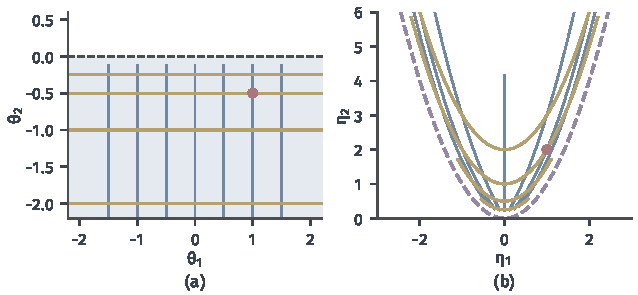
\includegraphics[width=108mm]{figures/07-probability/04-distribution-analysis/matplotlib/dfam-mean-map/figure.pdf}
  \caption{高斯族的自然参数与均值参数。(a)自然参数域是半平面$\theta_2<0$（浅蓝），画出直线族$\theta_1=$常数（蓝）与$\theta_2=$常数（黄）。(b)它们经$\nabla A$映到抛物线$\eta_2=\eta_1^{2}$（紫色虚线）上方的区域。红点是$\mathcal{N}(1,1)$：$\bm{\theta}=(1,-\frac12)$，$\bm{\eta}=(1,2)$。抛物线本身对应点质量，不在像中。}
  \label{fig:dfam-mean-map}
\end{BookInlineFigure}

\paragraph{对应的范围}
定理~\ref{thm:dfam-natural-mean}的坐标对应只在正则族的参数域与均值映射的像$\mathcal{M}^{\circ}$之间成立。它不覆盖可行均值的边界，也不覆盖非正则族的边界参数：第~\ref{sec:dfam-natural-domain}节中$h=(1+x)^{-2}$的族，边界点$\theta=0$在参数域中，那里却没有有限的均值参数。给定一个均值时是否存在族中的分布、存在时怎样求出对应的自然参数，以及在$\mathcal{M}^{\circ}$之外怎样处理，是第~\ref{chap:distribution-selection}章矩匹配的问题；两套坐标之间更细的几何关系由第~\ref{chap:information-geometry}章展开。


\section{本章小结}
\label{sec:dfam-summary}

章首的问题是：在挑选一个分布之前，怎样说清允许哪些分布、怎样给它们编号。第一节把这两件事分开。候选范围由支撑、矩约束和相对参考测度的绝对连续性规定，它们限制的是概率规律本身；三面骰子的候选集合是三角形中的线段，给定均值的密度却多到不能用有限个系数线性表示。参数化是从参数到分布的映射，可辨识性问的是这个映射是否为单射。重复参数、只以组合出现的参数和标签置换都会破坏可辨识性；可辨识只是分布层面的唯一性，不等于有限样本能准确分辨参数。

后四节给出四种构造。它们固定的对象与可调的参数不同，表~\ref{tab:dfam-constructions}把它们并排列出。

\begin{BookInlineTable}
  \centering
  \caption{四种构造分布族的方式}
  \label{tab:dfam-constructions}
  \begin{tabular}{@{}llll@{}}
    \toprule
    构造 & 固定的对象 & 随参数变化的部分 & 需要核对的条件\\
    \midrule
    推前 & 基础分布$P_0$ & 映射$T_{\bm{\theta}}$ & 密度是否存在\\
    混合 & 核或成分族 & 混合测度、成分参数 & 表示是否唯一\\
    Copula & 依赖结构$C$ & 边缘分布$F_i$ & 边缘是否连续\\
    指数族 & $h\nu$与$\bm{T}$ & 自然参数$\bm{\theta}$ & 参数域与最小性\\
    \bottomrule
  \end{tabular}
\end{BookInlineTable}

推前族把随机性放在固定的基础分布里，参数只控制映射。位置尺度族中分布函数与分位数按仿射规律变化，矩在存在时随之变化，标准化后的形状保持不变；固定基础分布后，非退化的基础变量使位置与尺度可辨识。非线性可逆映射改变形状，低维随机性进入高维空间使支撑退化而失去密度，离散化产生原子。只有同维可逆光滑的映射才能直接用Jacobian公式写出密度，一般的推前族要用推前测度和基础空间上的期望来描述。

混合族按随机选出的成分产生结果，有限混合是概率的加权平均，而不是取值的加权平均。两个高斯成分足够分开时出现双峰，这是成分族自身没有的形状；改权重只在固定形状之间重新分配质量，改成分参数才改变形状。连续混合把求和换成对混合测度的积分：正态尺度混合的峰度不小于$3$，多元时共同尺度使分量不相关却不独立；Poisson–Gamma混合得到方差更大的负二项分布。混合表示有标签置换、重复成分与零权重三种冗余，成分重叠本身并不是冗余：已知方差的高斯位置混合除标签置换外可辨识，Bernoulli成分的混合却完全不可辨识。

Copula把联合分布拆成边缘与依赖。Sklar定理说任何Copula可以与任何边缘拼成联合分布，任何联合分布都有Copula；边缘连续时，概率积分变换把各分量送到均匀刻度，Copula唯一，并且在分量的严格递增变换下不变。边缘有原子时，Copula只在边缘分布函数值域的乘积上确定，两枚独立硬币可以配上看起来很不一样的Copula，分布变换仍能保证存在性。

指数族对若干统计量施加指数权重，基准测度与统计量固定，自然参数在使配分积分有限的凸集上变化。参数域内部，对数配分函数的梯度与Hessian给出统计量的均值与协方差，凸性由协方差的半正定性解释，严格凸性要求统计量之间没有仿射关系。最小表示下参数可辨识；正则族中均值映射是从自然参数域到一个开集的连续可微双射，但这个开集不含可行均值的边界，参数趋于无穷时分布可能趋于族外的点质量，非正则族的边界参数也可能没有有限均值。

这四种构造可以描述同一个分布族。高斯族既是标准高斯的位置尺度族，又是以$(x,x^{2})$为统计量的指数族；多元高斯分布既是标准高斯向量的仿射推前，也可以拆成高斯边缘加上高斯Copula；Laplace分布既是位置尺度族，又是正态尺度混合。选用哪一种表示，取决于要回答的问题：生成样本时推前最方便，解释异质来源时混合最自然，分开处理边缘与依赖时用Copula，需要用矩刻画分布时用指数族。

本章只建立了候选族的表示与可辨识性。给定约束后在全体允许的分布中选出哪一个，指数族会作为最优解的形式出现，这是第~\ref{chap:distribution-selection}章的内容；把候选限制在某个族之后，怎样在族内逼近一个给定的分布、误差有多大，由第~\ref{chap:distribution-approximation}章研究。


\chapter{概率分布的比较}
\label{chap:distribution-comparison}

某个随机结果只取$0,1,2$三个值，关于它有两份概率表：
\[
 P=(0.6,\ 0.3,\ 0.1),\qquad Q=(0.3,\ 0.3,\ 0.4) .
\]
$P$是我们相信的规律，$Q$是另一个人给出的规律。两张表差多少？这个问题没有唯一的答案，答案取决于差别会在哪里造成后果。若关心的是某件事发生的概率，最坏的事件是“掷出$0$”，两边相差$0.3$。若用$Q$去预测按$P$产生的结果，要看的是$Q$在$P$常出现的地方给的概率是否太小，这牵涉到两表在同一点上的比值。若关心的是取值的平均，$P$下是$0.5$，$Q$下是$1.1$，相差$0.6$。若把取值看成直线上的位置，要把$P$的概率质量搬成$Q$的样子，搬动的质量乘以距离，总量至少是$0.6$。

再看一个更极端的例子。两个单点分布$\delta_0$与$\delta_h$，$h$是很小的正数。按事件看，它们完全不同：事件$\{0\}$在前者下概率为$1$，在后者下为$0$。按位置看，它们只差一个小平移。哪种看法对，取决于后续要用这个比较做什么：控制事件概率，控制似然比，控制某类函数的平均，还是控制位置的移动。

本章依次建立这四个角度的比较量。第一节用同一事件的概率差定义总变差，并把它写成密度差的积分和有界函数的期望差。第二节在同一参考测度下比较密度，得到KL散度、Hellinger距离、JS散度、$f$散度与Rényi散度，并证明随机后处理不会增大$f$散度。第三节用一类测试函数的期望差比较分布，核心是再生核Hilbert空间给出的核均值与MMD。第四节用耦合定义Wasserstein距离，并对一阶距离给出Lipschitz函数表示。

这四个角度互有交叉：总变差同时是事件比较、密度比较和有界函数比较，一阶Wasserstein距离同时是运输成本和Lipschitz函数比较。第五节固定一个评价函数，按它的有界性、Lipschitz性、RKHS范数或指数矩选用合适的比较量，给出期望误差的上界，并说明无界函数必须补充尾部条件。第六节研究一列分布的比较量趋于零能推出什么，把它们与第~\ref{chap:weak-convergence-of-distributions}章的弱收敛联系起来。

本章使用第~\ref{chap:probability-spaces}章的测度语言和Radon–Nikodym密度，第~\ref{chap:conditional-expectation}章的条件期望与条件Jensen不等式，以及第~\ref{chap:weak-convergence-of-distributions}章的弱收敛。分布由单个总体规律给出，本章不讨论怎样从样本估计这些量。

\section{总变差}
\label{sec:dcomp-tv}

最直接的比较是逐个事件对照：同一个事件$A$，在一个分布下概率是$P(A)$，在另一个分布下是$Q(A)$。只要所有事件的概率差都小，用$Q$代替$P$去回答“某事发生的概率是多少”就不会出大错。把所有事件中最坏的那个差拿出来，就得到一个数。本节先给出这个数的定义和计算方法，再把它从事件推广到有界函数的平均。

全章设$P,Q$是同一个可测空间$(\mathcal{X},\mathcal{F}_{\mathcal{X}})$上的概率测度。$\mathcal{X}$可以是有限集、$\mathbb{R}^{d}$或其他取值空间，事件指$\mathcal{F}_{\mathcal{X}}$中的集合。

\subsection{定义与计算}
\label{sec:dcomp-tv-definition}

把每个事件上的概率差取绝对值，再在全体事件上取上确界，就得到总变差。

\begin{definition}[总变差]
\label{def:dcomp-tv}
$P$与$Q$之间的\term{总变差}（total variation distance）是
\begin{equation}
 d_{\mathrm{TV}}(P,Q)=\sup_{A\in\mathcal{F}_{\mathcal{X}}}\bigl\lvert P(A)-Q(A)\bigr\rvert .
 \label{eq:dcomp-tv-def}
\end{equation}
\end{definition}

由定义可以直接读出几条性质。每个概率差都在$[-1,1]$中，所以$0\leq d_{\mathrm{TV}}\leq1$。交换$P,Q$不改变绝对值，所以它对称。对第三个分布$R$与任一事件$A$，
\[
 \lvert P(A)-R(A)\rvert\leq\lvert P(A)-Q(A)\rvert+\lvert Q(A)-R(A)\rvert ,
\]
两边取上确界得到三角不等式。$d_{\mathrm{TV}}(P,Q)=0$表示每个事件的概率都相同，即$P=Q$。所以总变差是全体概率测度上的一个距离。

\paragraph{有限概率表}
先在章首的例子上计算。$\mathcal{X}=\{0,1,2\}$，两份概率表是
\[
 p=(0.6,\ 0.3,\ 0.1),\qquad q=(0.3,\ 0.3,\ 0.4) .
\]
下文称它为\emph{例表}。三个点有$8$个子集，逐个计算$P(A)-Q(A)$，结果列在表~\ref{tab:dcomp-tv-events}中。差最大的是$\{0\}$与$\{0,1\}$，都等于$0.3$；最小的是$\{2\}$与$\{1,2\}$，都等于$-0.3$。所以$d_{\mathrm{TV}}(P,Q)=0.3$。

\begin{BookInlineTable}
 \centering
 \caption{例表中每个事件的概率差。}
 \label{tab:dcomp-tv-events}
 \begin{tabular}{lcccccccc}
  \toprule
  $A$ & $\varnothing$ & $\{0\}$ & $\{1\}$ & $\{2\}$ & $\{0,1\}$ & $\{0,2\}$ & $\{1,2\}$ & $\mathcal{X}$\\
  \midrule
  $P(A)-Q(A)$ & $0$ & $0.3$ & $0$ & $-0.3$ & $0.3$ & $0$ & $-0.3$ & $0$\\
  \bottomrule
 \end{tabular}
\end{BookInlineTable}

表中有规律可循。事件的概率差是各点概率差之和，点$0$贡献$+0.3$，点$1$贡献$0$，点$2$贡献$-0.3$。要让和最大，就把所有贡献为正的点放进事件，把贡献为负的点排除在外，见图~\ref{fig:dcomp-tv-table}。最坏事件是$\{x:p(x)>q(x)\}$，最大的差等于正的差之和。又因为两表各自总和为$1$，正的差之和等于负的差之和的绝对值，各占全部绝对差的一半：
\[
 d_{\mathrm{TV}}(P,Q)=\tfrac12\bigl(\lvert0.3\rvert+\lvert0\rvert+\lvert-0.3\rvert\bigr)=0.3 .
\]

\begin{BookInlineFigure}
 \centering
 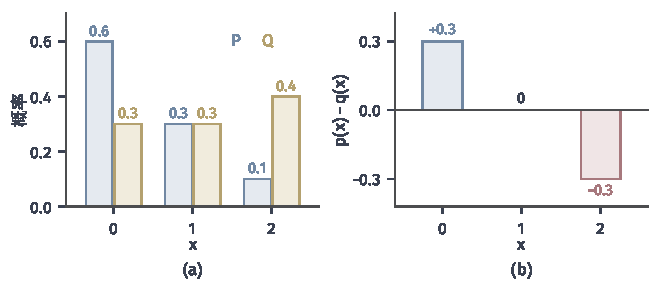
\includegraphics[width=112mm]{figures/07-probability/04-distribution-analysis/matplotlib/dcomp-tv-table/figure.pdf}
 \caption{例表的总变差。(a)蓝色柱为$P$，黄色柱为$Q$。(b)逐点概率差$p(x)-q(x)$，蓝色为正，红色为负。正的部分之和与负的部分之和的绝对值相等，都是$0.3$，即$d_{\mathrm{TV}}(P,Q)$。}
 \label{fig:dcomp-tv-table}
\end{BookInlineFigure}

\paragraph{共同支配测度}
要把这个规律推广到一般分布，需要一个能同时描述$P$与$Q$的“逐点概率”。有限表里它就是概率表本身；连续情形是密度；混有原子时两者都不够用。统一的办法是找一个测度$\lambda$，使$P,Q$都相对于它有密度。设$\lambda$是$\sigma$有限测度，并且$P\ll\lambda$，$Q\ll\lambda$，即$\lambda(A)=0$时$P(A)=Q(A)=0$。由Radon–Nikodym定理，存在非负可测函数$p,q$使
\begin{equation}
 P(A)=\int_{A}p\,\mathrm{d}\lambda,\qquad Q(A)=\int_{A}q\,\mathrm{d}\lambda,\qquad A\in\mathcal{F}_{\mathcal{X}},
 \label{eq:dcomp-common-density}
\end{equation}
并且$p,q$在$\lambda$几乎处处的意义下唯一，可参考\BookChapterRef{chap:measure-densities}{卷四第8章“测度的密度”}。这样的$\lambda$称为$P$与$Q$的\term{支配测度}（dominating measure），$p,q$称为它们相对于$\lambda$的密度。下文写$p,q$时，总是指相对于某个共同支配测度的密度。

支配测度总是存在：取$\lambda=P+Q$即可，因为$\lambda(A)=0$迫使$P(A)=Q(A)=0$。在有限表上$\lambda$取计数测度，$p,q$就是概率表；在$\mathbb{R}^{d}$上两者都有普通密度时，$\lambda$取Lebesgue测度。

\begin{theorem}[总变差的密度表示]
\label{thm:dcomp-tv-density}
设$p,q$是$P,Q$相对于共同支配测度$\lambda$的密度，$A^{*}=\{x:p(x)>q(x)\}$。则
\begin{equation}
 d_{\mathrm{TV}}(P,Q)=\frac12\int\lvert p-q\rvert\,\mathrm{d}\lambda=P(A^{*})-Q(A^{*})=1-\int\min(p,q)\,\mathrm{d}\lambda .
 \label{eq:dcomp-tv-density}
\end{equation}
\end{theorem}

\begin{proof}
先说明$A^{*}$达到上确界。对任一事件$A$，把它拆成$A\cap A^{*}$与$A\setminus A^{*}$。在$A^{*}$上$p-q>0$，在其外$p-q\leq0$，所以
\[
 P(A)-Q(A)=\int_{A}(p-q)\,\mathrm{d}\lambda\leq\int_{A\cap A^{*}}(p-q)\,\mathrm{d}\lambda\leq\int_{A^{*}}(p-q)\,\mathrm{d}\lambda .
\]
第一步丢掉了非正的部分，第二步补上了非负的部分。右端就是$P(A^{*})-Q(A^{*})$。同理，$Q(A)-P(A)\leq Q(B)-P(B)$，其中$B=(A^{*})^{\mathrm{c}}$。

再说明两个方向的最大值相等。两个密度的积分都是$1$，所以$\int(p-q)\,\mathrm{d}\lambda=0$，把积分拆到$A^{*}$与$B$上，得到
\[
 \int_{A^{*}}(p-q)\,\mathrm{d}\lambda=\int_{B}(q-p)\,\mathrm{d}\lambda .
\]
因此$\lvert P(A)-Q(A)\rvert$的上确界等于$P(A^{*})-Q(A^{*})$，即式~\eqref{eq:dcomp-tv-density}的第二个表达式。

$\lvert p-q\rvert$在$A^{*}$上等于$p-q$，在$B$上等于$q-p$。由上式，两部分积分相等，所以$\int\lvert p-q\rvert\,\mathrm{d}\lambda$是它们的两倍，这给出第一个表达式。最后，由$\lvert p-q\rvert=p+q-2\min(p,q)$，
\[
 \frac12\int\lvert p-q\rvert\,\mathrm{d}\lambda=\frac12\Bigl(1+1-2\int\min(p,q)\,\mathrm{d}\lambda\Bigr)=1-\int\min(p,q)\,\mathrm{d}\lambda .
\]
\end{proof}

式~\eqref{eq:dcomp-tv-density}的左端按定义~\eqref{eq:dcomp-tv-def}计算，与$\lambda$无关，所以右端也与支配测度的选取无关。最后一个表达式给出一个面积图景：$\int\min(p,q)\,\mathrm{d}\lambda$是两个密度的重叠部分，总变差是$1$减去重叠，也就是一个分布中“没有被另一个分布覆盖”的质量。

\paragraph{两个高斯分布}
取$P=\mathcal{N}(0,1)$，$Q=\mathcal{N}(1,1)$，以Lebesgue测度为支配测度。两个密度在$x=1/2$处相等，左侧$p>q$，所以$A^{*}=(-\infty,1/2)$。由式~\eqref{eq:dcomp-tv-density}，
\[
 d_{\mathrm{TV}}(P,Q)=\Phi\Bigl(\frac12\Bigr)-\Phi\Bigl(\frac12-1\Bigr)=2\Phi\Bigl(\frac12\Bigr)-1\approx0.3829 .
\]
图~\ref{fig:dcomp-tv-gaussians}(a)中浅蓝区域的面积是$\int(p-q)^{+}\,\mathrm{d}x$，浅黄区域是$\int(q-p)^{+}\,\mathrm{d}x$，两块面积相等，都是总变差。

\paragraph{没有共同普通密度的情形}
取
\[
 P=\operatorname{Unif}(0,1),\qquad Q=\tfrac12\operatorname{Unif}(0,1)+\tfrac12\delta_{1/2},
\]
即$Q$以一半概率均匀取值，另一半概率恰好取$1/2$。$Q$在单点$1/2$上有正概率，它没有Lebesgue密度。取$\lambda$为$(0,1)$上的Lebesgue测度加上$1/2$处的单位点质量，两个分布都被它支配，密度是
\[
 p(x)=\begin{cases}1,&x\in(0,1)\setminus\{\tfrac12\},\\0,&x=\tfrac12,\end{cases}\qquad
 q(x)=\begin{cases}\tfrac12,&x\in(0,1)\setminus\{\tfrac12\},\\\tfrac12,&x=\tfrac12 .\end{cases}
\]
在$x=1/2$处，$p$取$0$是因为$P(\{1/2\})=0$，而这一点上$\lambda$的质量是$1$，$q$必须等于$Q(\{1/2\})=1/2$。由式~\eqref{eq:dcomp-tv-density}，
\[
 d_{\mathrm{TV}}(P,Q)=\frac12\Bigl(\int_0^1\Bigl\lvert1-\frac12\Bigr\rvert\,\mathrm{d}x+\Bigl\lvert0-\frac12\Bigr\rvert\Bigr)=\frac12 .
\]
直接用定义检验：事件$\{1/2\}$的概率差就是$1/2$。图~\ref{fig:dcomp-tv-gaussians}(b)把原子画成竖线，它相对于$\lambda$的“密度”是该点的概率。

\begin{BookInlineFigure}
 \centering
 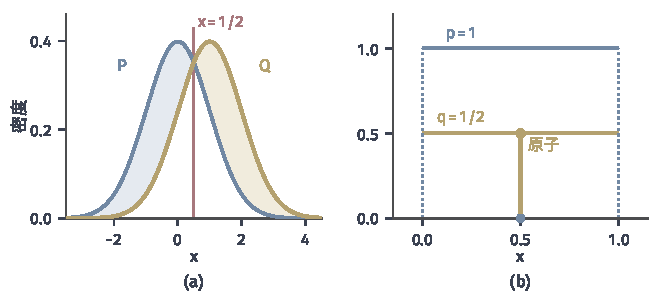
\includegraphics[width=112mm]{figures/07-probability/04-distribution-analysis/matplotlib/dcomp-tv-gaussians/figure.pdf}
 \caption{总变差的计算。(a)$P=\mathcal{N}(0,1)$（蓝）与$Q=\mathcal{N}(1,1)$（黄），红线是$x=1/2$；浅蓝区域$\{p>q\}$与浅黄区域$\{q>p\}$的面积都等于$d_{\mathrm{TV}}(P,Q)\approx0.3829$。(b)$P=\operatorname{Unif}(0,1)$（蓝）与$Q=\tfrac12\operatorname{Unif}(0,1)+\tfrac12\delta_{1/2}$（黄）相对于“Lebesgue测度加$1/2$处点质量”的密度；黄色竖线是$Q$在$1/2$处的原子，蓝点表示$P$在该点的密度为$0$。}
 \label{fig:dcomp-tv-gaussians}
\end{BookInlineFigure}

\paragraph{总变差看不到距离}
单点分布$\delta_x$与$\delta_y$（$x\neq y$）的总变差总是$1$：事件$\{x\}$在前者下概率为$1$，在后者下为$0$。无论$x,y$相距多近，结果都一样。更一般地，若存在事件$A$使$P(A)=1$，$Q(A)=0$，即$P$与$Q$相互奇异，则$d_{\mathrm{TV}}(P,Q)=1$，取到最大值。总变差只问“同一个事件的概率是否相同”，不问取值之间有多远。第~\ref{sec:dcomp-wasserstein}节会用位置移动的成本补上这个缺口。

\subsection{有界函数的期望差}
\label{sec:dcomp-tv-functions}

事件的概率是示性函数的期望：$P(A)=\mathbb{E}_{P}[\mathbf{1}_{A}]$。若关心的不是某件事是否发生，而是一个有界的数值结果，例如有上限的损失，那么要比较的是$\mathbb{E}_{P}[g]$与$\mathbb{E}_{Q}[g]$。总变差同样能控制它们，只是系数取决于$g$的取值范围。

\begin{theorem}[有界函数的期望差]
\label{thm:dcomp-tv-bounded}
设$g:\mathcal{X}\to\mathbb{R}$可测且有界，记$\operatorname{osc}(g)=\sup g-\inf g$。则
\begin{equation}
 \bigl\lvert\mathbb{E}_{P}[g]-\mathbb{E}_{Q}[g]\bigr\rvert\leq\operatorname{osc}(g)\,d_{\mathrm{TV}}(P,Q)\leq2\lVert g\rVert_{\infty}\,d_{\mathrm{TV}}(P,Q),
 \label{eq:dcomp-tv-osc}
\end{equation}
其中$\lVert g\rVert_{\infty}=\sup\lvert g\rvert$。并且
\begin{equation}
 \sup_{\lVert g\rVert_{\infty}\leq1}\bigl\lvert\mathbb{E}_{P}[g]-\mathbb{E}_{Q}[g]\bigr\rvert=2\,d_{\mathrm{TV}}(P,Q),
 \label{eq:dcomp-tv-dual}
\end{equation}
上确界在$g^{\pm}$处达到，$g^{\pm}$在$A^{*}$上取$1$，在其外取$-1$。
\end{theorem}

\begin{proof}
用共同支配测度写出期望差$\int g\,(p-q)\,\mathrm{d}\lambda$。因为$\int(p-q)\,\mathrm{d}\lambda=0$，被积函数中的$g$可以减去任意常数$c$而不改变积分：
\[
 \mathbb{E}_{P}[g]-\mathbb{E}_{Q}[g]=\int\bigl(g-c\bigr)(p-q)\,\mathrm{d}\lambda .
\]
取$c=(\sup g+\inf g)/2$，则$\lvert g-c\rvert\leq\operatorname{osc}(g)/2$处处成立。于是
\[
 \bigl\lvert\mathbb{E}_{P}[g]-\mathbb{E}_{Q}[g]\bigr\rvert\leq\frac{\operatorname{osc}(g)}{2}\int\lvert p-q\rvert\,\mathrm{d}\lambda=\operatorname{osc}(g)\,d_{\mathrm{TV}}(P,Q),
\]
最后一步用了式~\eqref{eq:dcomp-tv-density}。又$\operatorname{osc}(g)\leq2\lVert g\rVert_{\infty}$，得到式~\eqref{eq:dcomp-tv-osc}。

对$\lVert g\rVert_{\infty}\leq1$，上式给出期望差不超过$2d_{\mathrm{TV}}$。取$g=g^{\pm}$，则$g(p-q)=\lvert p-q\rvert$，期望差恰好是$\int\lvert p-q\rvert\,\mathrm{d}\lambda$，即$2d_{\mathrm{TV}}$，所以式~\eqref{eq:dcomp-tv-dual}的上确界达到。
\end{proof}

减去常数这一步是关键。概率差只对“质量怎样重新分配”敏感，整体平移$g$不影响结果，所以真正起作用的是$g$的振幅$\operatorname{osc}(g)$，而不是它的绝对大小。

\paragraph{系数的两种约定}
定义~\eqref{eq:dcomp-tv-def}在事件上取上确界，等价于在取值于$[0,1]$的函数上取上确界：这样的$g$满足$\operatorname{osc}(g)\leq1$，由式~\eqref{eq:dcomp-tv-osc}，期望差不超过$d_{\mathrm{TV}}$，而示性函数$\mathbf{1}_{A^{*}}$达到它。若改在单位球$\lVert g\rVert_{\infty}\leq1$上取上确界，函数可以从$-1$变到$1$，振幅加倍，结果是$2d_{\mathrm{TV}}$。有些文献把$\int\lvert p-q\rvert\,\mathrm{d}\lambda$称为总变差，它是本书$d_{\mathrm{TV}}$的两倍。读到“总变差小于$\varepsilon$”时，要先确认用的是哪一种约定。

\paragraph{例表上的检验}
在例表上取$g=g^{\pm}$。这里$A^{*}=\{0\}$，$g$在三个点上依次取$1,-1,-1$，两个期望是
\[
 \mathbb{E}_{P}[g]=0.6-0.3-0.1=0.2,\qquad\mathbb{E}_{Q}[g]=0.3-0.3-0.4=-0.4 .
\]
差为$0.6$，正是$2d_{\mathrm{TV}}$。再取$g(x)=x$，它的振幅是$2$，式~\eqref{eq:dcomp-tv-osc}给出的上界与实际的差分别是
\[
 2\times0.3=0.6,\qquad\lvert0.5-1.1\rvert=0.6,
\]
上界恰好达到。原因是$x=1-\tilde{g}(x)$，其中$\tilde{g}$在三点上依次取$1,0,-1$，而$\tilde{g}$正好在$p>q$处取最大值、在$p<q$处取最小值。一般的有界函数没有这样的巧合，上界会有余量。

式~\eqref{eq:dcomp-tv-dual}把总变差写成一类测试函数上的最大期望差。第~\ref{sec:dcomp-ipm}节会换用别的函数类得到别的比较量，第~\ref{sec:dcomp-expectation}节会把这个结果与其他比较量的类似结果放在一起，按评价函数的性质选择。

\section{密度比较}
\label{sec:dcomp-density}

总变差只用到密度之差$\lvert p-q\rvert$。看两个位置：一处$p=0.02$，$q=0.01$；另一处$p=0.51$，$q=0.50$。两处的差都是$0.01$，对总变差的贡献相同。可是若用$Q$去预测按$P$产生的结果，第一处的结果实际出现的频率是$Q$所说的两倍，第二处只多了百分之二。比值$p(x)/q(x)$记录的正是这种相对失衡。

本节在同一个支配测度$\lambda$下比较同一位置上的两个密度，用对数比、平方根和幂次构造几种比较量，再把它们归入同一个机制：对密度比施加一个凸函数，再求平均。密度为零的位置需要单独约定，而且多数比较量不对称或不满足三角不等式，所以统称为散度，只有满足距离公理的才称为距离。

\subsection{KL散度}
\label{sec:dcomp-kl}

\paragraph{对数比的平均}
设观测到一个结果$x$，要判断它更像来自$P$还是$Q$。比值$p(x)/q(x)$大于$1$时支持$P$，取对数后$\ln(p(x)/q(x))$大于零。对数的好处是独立观测的证据可以相加：$n$次独立观测的密度比是各次比值的乘积，取对数就成了各次对数比之和。如果数据确实来自$P$，每次观测平均提供的证据是对数比在$P$下的期望。由第~\ref{chap:laws-of-large-numbers}章的强大数律，只要这个期望存在，$n$次观测的总证据除以$n$几乎必然趋于它，所以它衡量的是“$P$为真时，平均每次观测能把$P$与$Q$分开多少”。

对数比在$q(x)=0<p(x)$处是$+\infty$：$P$下可能出现、$Q$却认为不可能的结果，一旦出现就彻底否定$Q$。在$p(x)=0$处，这个点在$P$下不出现，对平均没有贡献。定义据此处理零密度。

\begin{definition}[KL散度]
\label{def:dcomp-kl}
设$p,q$是$P,Q$相对于共同支配测度$\lambda$的密度。若$P\ll Q$，定义$P$相对于$Q$的\term{KL散度}（Kullback--Leibler divergence）为
\begin{equation}
 D_{\mathrm{KL}}(P\Vert Q)=\int_{\{p>0\}}p\ln\frac{p}{q}\,\mathrm{d}\lambda=\mathbb{E}_{P}\Bigl[\ln\frac{\mathrm{d}P}{\mathrm{d}Q}\Bigr] ;
 \label{eq:dcomp-kl-def}
\end{equation}
若$P$不绝对连续于$Q$，定义$D_{\mathrm{KL}}(P\Vert Q)=+\infty$。
\end{definition}

定义里有两件事需要核对。第一，积分有意义。$P\ll Q$时$P(q=0)=0$，被积函数在$\{p>0\}$上$\lambda$几乎处处有限。它的负部只出现在$p<q$处，由$\ln u\leq u-1$，
\[
 \int_{\{0<p<q\}}p\ln\frac{q}{p}\,\mathrm{d}\lambda\leq\int_{\{0<p<q\}}p\Bigl(\frac{q}{p}-1\Bigr)\,\mathrm{d}\lambda\leq\int q\,\mathrm{d}\lambda=1 .
\]
负部的积分有限，所以整个积分在$(-\infty,+\infty]$中有确定的值。第二，结果与$\lambda$无关：$P\ll Q$时比值$p/q$在$P$几乎处处的意义下就是Radon–Nikodym密度$\mathrm{d}P/\mathrm{d}Q$，式~\eqref{eq:dcomp-kl-def}的最后一个表达式里没有$\lambda$。

\begin{theorem}[Gibbs不等式]
\label{thm:dcomp-gibbs}
$D_{\mathrm{KL}}(P\Vert Q)\geq0$，等号成立当且仅当$P=Q$。
\end{theorem}

\begin{proof}
若$P$不绝对连续于$Q$，散度为$+\infty$，结论成立。设$P\ll Q$。在$\{p>0\}$上用$\ln u\leq u-1$（等号仅在$u=1$时成立），取$u=q/p$，
\[
 -D_{\mathrm{KL}}(P\Vert Q)=\int_{\{p>0\}}p\ln\frac{q}{p}\,\mathrm{d}\lambda\leq\int_{\{p>0\}}(q-p)\,\mathrm{d}\lambda=Q(p>0)-1\leq0 .
\]
若等号成立，第一个不等号要求$\lambda$几乎处处在$\{p>0\}$上$q=p$，第二个要求$Q(p>0)=1$，即$Q$在$\{p=0\}$上没有质量。两条合起来就是$p=q$几乎处处，即$P=Q$。
\end{proof}

这个结论称为\term{Gibbs不等式}（Gibbs' inequality）。证明里用的$\ln u\leq u-1$是对数函数位于它在$u=1$处切线下方，即凹性。KL散度非负，是因为在$P$自己的权重下，“用$Q$的概率”平均起来不如“用$P$自己的概率”。

\paragraph{方向不对称}
在例表上逐项计算。点$1$处$p=q$，贡献为零；另外两项是
\[
 0.6\ln\frac{0.6}{0.3}=0.6\ln2,\qquad 0.1\ln\frac{0.1}{0.4}=-0.2\ln2 .
\]
两项相加，
\[
 D_{\mathrm{KL}}(P\Vert Q)=0.4\ln2\approx0.2773 .
\]
交换两表，同样的两个位置贡献$0.3\ln(1/2)=-0.3\ln2$与$0.4\ln4=0.8\ln2$，
\[
 D_{\mathrm{KL}}(Q\Vert P)=0.5\ln2\approx0.3466 .
\]
两个方向的数值不同。单项可以为负（例如点$2$处$p<q$），总和却不为负，这正是Gibbs不等式。图~\ref{fig:dcomp-kl-asymmetry}(a)画出各项的贡献：$D_{\mathrm{KL}}(Q\Vert P)$的大头来自点$2$，那里$Q$有$0.4$的质量而$P$只给$0.1$。

\paragraph{高斯分布}
取$P=\mathcal{N}(\mu_1,\sigma_1^{2})$，$Q=\mathcal{N}(\mu_2,\sigma_2^{2})$。两个密度之比的对数是
\[
 \ln\frac{p(x)}{q(x)}=\ln\frac{\sigma_2}{\sigma_1}-\frac{(x-\mu_1)^{2}}{2\sigma_1^{2}}+\frac{(x-\mu_2)^{2}}{2\sigma_2^{2}} .
\]
在$P$下取期望，$\mathbb{E}_{P}[(X-\mu_1)^{2}]=\sigma_1^{2}$，而
\[
 \mathbb{E}_{P}\bigl[(X-\mu_2)^{2}\bigr]=\sigma_1^{2}+(\mu_1-\mu_2)^{2} .
\]
代入得到
\begin{equation}
 D_{\mathrm{KL}}(P\Vert Q)=\ln\frac{\sigma_2}{\sigma_1}+\frac{\sigma_1^{2}+(\mu_1-\mu_2)^{2}}{2\sigma_2^{2}}-\frac12 .
 \label{eq:dcomp-kl-gauss}
\end{equation}
方差相同时它化为$(\mu_1-\mu_2)^{2}/(2\sigma^{2})$，两个方向相等。尺度不同时不对称。图~\ref{fig:dcomp-kl-asymmetry}(b)固定$P=\mathcal{N}(0,1)$，令$Q_s=\mathcal{N}(0,s^{2})$。$s<1$时$Q_s$比$P$窄，$P$在两侧尾部的质量落在$Q_s$密度极小的地方，$D_{\mathrm{KL}}(P\Vert Q_s)$迅速增大；反过来，$D_{\mathrm{KL}}(Q_s\Vert P)$在$s<1$时保持较小。KL散度惩罚的是：参考分布$Q$在$P$有质量的地方给出太小的概率。

\begin{BookInlineFigure}
 \centering
 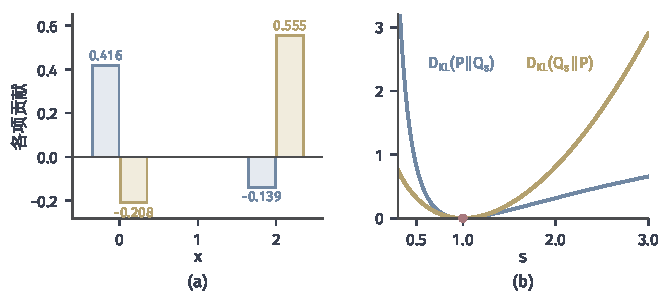
\includegraphics[width=112mm]{figures/07-probability/04-distribution-analysis/matplotlib/dcomp-kl-asymmetry/figure.pdf}
 \caption{KL散度的方向。(a)例表中各点的贡献：蓝色为$p\ln(p/q)$，合计$0.4\ln2\approx0.2773$；黄色为$q\ln(q/p)$，合计$0.5\ln2\approx0.3466$。(b)$P=\mathcal{N}(0,1)$，$Q_s=\mathcal{N}(0,s^{2})$，蓝线为$D_{\mathrm{KL}}(P\Vert Q_s)$，黄线为$D_{\mathrm{KL}}(Q_s\Vert P)$，红点是$s=1$。}
 \label{fig:dcomp-kl-asymmetry}
\end{BookInlineFigure}

\paragraph{绝对连续不保证有限}
$P\ll Q$只排除了“$Q$认为不可能、$P$却可能”的事件，并不保证对数比的平均有限。取$P$为标准Cauchy分布，$Q=\mathcal{N}(0,1)$。两个密度处处为正，互相绝对连续。对数比为
\[
 \ln\frac{p(x)}{q(x)}=\frac{x^{2}}{2}-\ln\bigl(1+x^{2}\bigr)+\ln\sqrt{\frac{2}{\pi}} .
\]
当$\lvert x\rvert$足够大时，右边不小于$x^{2}/4$，而Cauchy分布下$\mathbb{E}_{P}[X^{2}]=+\infty$，所以$D_{\mathrm{KL}}(P\Vert Q)=+\infty$。反方向的散度是对数比的相反数在$\mathcal{N}(0,1)$下的期望，其中$X^{2}$与$\ln(1+X^{2})$都可积，所以$D_{\mathrm{KL}}(Q\Vert P)$有限。用尾部很轻的高斯分布去预测重尾的Cauchy结果，代价是无穷大；反过来则不然。

\subsection{Hellinger距离}
\label{sec:dcomp-hellinger}

KL散度不对称，可以是无穷大，并且对零密度极为敏感。若想要一个真正的距离，可以先把密度开平方。$\sqrt{p}$满足$\int(\sqrt{p})^{2}\,\mathrm{d}\lambda=1$，即它是$L^{2}(\lambda)$中的单位向量。于是每个分布对应单位球面上的一个点，两个分布之间可以用这两个点的欧氏距离比较。

\begin{definition}[Hellinger距离与Bhattacharyya系数]
\label{def:dcomp-hellinger}
设$p,q$是$P,Q$相对于共同支配测度$\lambda$的密度。称
\begin{equation}
 d_{\mathrm{H}}(P,Q)=\frac{1}{\sqrt2}\bigl\lVert\sqrt{p}-\sqrt{q}\bigr\rVert_{L^{2}(\lambda)}=\Bigl(\frac12\int\bigl(\sqrt{p}-\sqrt{q}\bigr)^{2}\,\mathrm{d}\lambda\Bigr)^{1/2}
 \label{eq:dcomp-hellinger-def}
\end{equation}
为\term{Hellinger距离}（Hellinger distance），称
\begin{equation}
 B(P,Q)=\int\sqrt{pq}\,\mathrm{d}\lambda
 \label{eq:dcomp-bhattacharyya-coefficient}
\end{equation}
为\term{Bhattacharyya系数}（Bhattacharyya coefficient）。
\end{definition}

把式~\eqref{eq:dcomp-hellinger-def}中的平方展开，两个密度的积分都是$1$，交叉项正是$B$：
\begin{equation}
 d_{\mathrm{H}}^{2}(P,Q)=\frac12\int\bigl(p+q-2\sqrt{pq}\bigr)\,\mathrm{d}\lambda=1-B(P,Q) .
 \label{eq:dcomp-hellinger-bc}
\end{equation}
由Cauchy--Schwarz不等式，$B$不超过$\sqrt{p}$与$\sqrt{q}$的$L^{2}$范数之积，即$1$；又$B\geq0$，所以$0\leq d_{\mathrm{H}}\leq1$。$d_{\mathrm{H}}=1$当且仅当$B=0$，即$pq=0$几乎处处，两个分布相互奇异。系数$1/\sqrt2$正是为了让最大值等于$1$。$d_{\mathrm{H}}$是$L^{2}(\lambda)$中两个向量之差的范数乘以常数，所以对称并满足三角不等式；$d_{\mathrm{H}}=0$表示$\sqrt{p}=\sqrt{q}$几乎处处，即$P=Q$。它是一个距离。

\paragraph{与支配测度无关}
定义用到了$\lambda$，需要检查换一个支配测度结果不变。设$\lambda$与$\lambda'$都支配$P,Q$。令$\nu=\lambda+\lambda'$，则$\lambda\ll\nu$，记$r=\mathrm{d}\lambda/\mathrm{d}\nu$。由密度的链式法则，$P,Q$相对于$\nu$的密度是$pr$与$qr$，于是
\[
 \int\sqrt{(pr)(qr)}\,\mathrm{d}\nu=\int\sqrt{pq}\,r\,\mathrm{d}\nu=\int\sqrt{pq}\,\mathrm{d}\lambda .
\]
所以用$\lambda$与用$\nu$算出的$B$相同。对$\lambda'$同样推理，三者一致。由式~\eqref{eq:dcomp-hellinger-bc}，$d_{\mathrm{H}}$也与支配测度无关。关键在于$\sqrt{pq}$关于密度是“一次齐次”的：密度整体乘以$r$，它也恰好乘以$r$，与积分测度的变化抵消。

\paragraph{例表与几何图景}
在例表上，
\[
 B(P,Q)=\sqrt{0.18}+\sqrt{0.09}+\sqrt{0.04}\approx0.4243+0.3+0.2=0.9243 .
\]
于是$d_{\mathrm{H}}^{2}\approx0.0757$，$d_{\mathrm{H}}\approx0.2752$。把$\sqrt{p}$与$\sqrt{q}$看成$\mathbb{R}^{3}$中的两个单位向量，$B$是它们的内积，也就是夹角$\theta$的余弦；这里$\theta\approx22.5^{\circ}$。$\sqrt2\,d_{\mathrm{H}}$是两个向量端点之间的弦长，见图~\ref{fig:dcomp-hellinger-roots}(b)。

\paragraph{两个高斯分布}
取方差同为$\sigma^{2}$、均值分别为$\mu_1,\mu_2$的两个高斯分布，记作$P$与$Q$，并记
\[
 \Delta=\mu_1-\mu_2,\qquad m=\tfrac12(\mu_1+\mu_2) .
\]
配方得到
\[
 (x-\mu_1)^{2}+(x-\mu_2)^{2}=2(x-m)^{2}+\frac{\Delta^{2}}{2} .
\]
代入两个密度的乘积再开方，$\sqrt{p(x)q(x)}$是以$m$为中心、方差为$\sigma^{2}$的高斯密度乘以常数
\[
 \exp\Bigl(-\frac{\Delta^{2}}{8\sigma^{2}}\Bigr) .
\]
高斯密度积分为$1$，于是
\begin{equation}
 B(P,Q)=\exp\Bigl(-\frac{(\mu_1-\mu_2)^{2}}{8\sigma^{2}}\Bigr) .
 \label{eq:dcomp-bc-gauss}
\end{equation}
图~\ref{fig:dcomp-hellinger-roots}(a)取$\sigma=1$，$\Delta=1.5$，浅蓝区域的面积是$B=\mathrm{e}^{-9/32}\approx0.7548$。重叠函数$\sqrt{pq}$的峰在两个均值的中点，两个分布离得越远，峰越低。

\begin{BookInlineFigure}
 \centering
 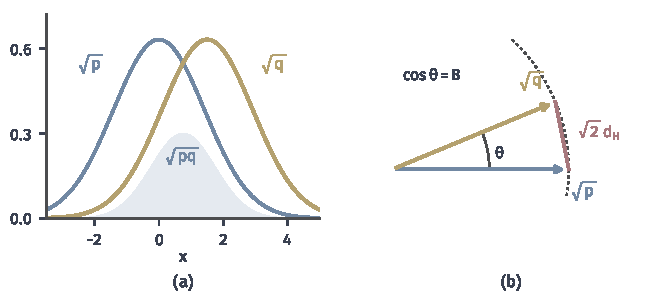
\includegraphics[width=112mm]{figures/07-probability/04-distribution-analysis/matplotlib/dcomp-hellinger-roots/figure.pdf}
 \caption{平方根密度。(a)$P=\mathcal{N}(0,1)$与$Q=\mathcal{N}(1.5,1)$的$\sqrt{p}$（蓝）与$\sqrt{q}$（黄），浅蓝区域是$\sqrt{pq}$，面积为$B\approx0.7548$。(b)例表的$\sqrt{\bm{p}}$与$\sqrt{\bm{q}}$是$\mathbb{R}^{3}$中的单位向量，画在它们张成的平面里；夹角$\theta\approx22.5^{\circ}$，$\cos\theta=B\approx0.9243$，红色弦长为$\sqrt2\,d_{\mathrm{H}}\approx0.389$。}
 \label{fig:dcomp-hellinger-roots}
\end{BookInlineFigure}

\paragraph{Bhattacharyya距离}
重叠系数的负对数
\begin{equation}
 D_{\mathrm{B}}(P,Q)=-\ln B(P,Q)
 \label{eq:dcomp-bhattacharyya-distance}
\end{equation}
称为\term{Bhattacharyya距离}（Bhattacharyya distance）。两个分布相互奇异时$B=0$，它等于$+\infty$，而$d_{\mathrm{H}}$此时只是$1$。$B$接近$1$时，$-\ln B\approx1-B=d_{\mathrm{H}}^{2}$。尽管名字里有“距离”，它不满足三角不等式。由式~\eqref{eq:dcomp-bc-gauss}，方差为$1$、均值分别为$0,1,2$的三个高斯分布两两之间的值是$\Delta^{2}/8$，于是
\[
 D_{\mathrm{B}}(\mathcal{N}(0,1),\mathcal{N}(2,1))=\frac12>\frac18+\frac18 .
\]
它随均值差平方增长，跨两步比走一步再走一步还“远”。在本章的用法里，$B$是重叠系数，$d_{\mathrm{H}}$是距离，$D_{\mathrm{B}}$只是$B$的一个单调变换。

\subsection{JS散度}
\label{sec:dcomp-js}

KL散度要求一个分布绝对连续于另一个。取$P=\operatorname{Unif}(0,1)$，$Q=\operatorname{Unif}(\tfrac12,\tfrac32)$，两个分布有一半质量重叠，可两个方向的KL散度都是$+\infty$：$P$在$(0,\tfrac12)$上有质量而$Q$没有，$Q$在$(1,\tfrac32)$上有质量而$P$没有。问题出在参考分布覆盖不到对方。一个自然的修补是换一个同时覆盖双方的参考分布，最简单的选择是两者的平均
\[
 M=\tfrac12(P+Q) .
\]
$M$的密度是$(p+q)/2$，只要$p>0$或$q>0$，它就为正。

\begin{definition}[JS散度]
\label{def:dcomp-js}
设$M=(P+Q)/2$。$P$与$Q$之间的\term{JS散度}（Jensen--Shannon divergence）是
\begin{equation}
 D_{\mathrm{JS}}(P,Q)=\frac12D_{\mathrm{KL}}(P\Vert M)+\frac12D_{\mathrm{KL}}(Q\Vert M) .
 \label{eq:dcomp-js-def}
\end{equation}
\end{definition}

用密度写出来，$\mathrm{d}P/\mathrm{d}M=2p/(p+q)$，所以
\[
 D_{\mathrm{JS}}(P,Q)=\frac12\int\Bigl(p\ln\frac{2p}{p+q}+q\ln\frac{2q}{p+q}\Bigr)\,\mathrm{d}\lambda ,
\]
其中$p=0$或$q=0$的项按$0\ln0=0$理解。

\begin{theorem}[JS散度的范围]
\label{thm:dcomp-js-range}
$D_{\mathrm{JS}}$对称，并且
\begin{equation}
 0\leq D_{\mathrm{JS}}(P,Q)\leq\ln2 .
 \label{eq:dcomp-js-range}
\end{equation}
左边等号成立当且仅当$P=Q$，右边等号成立当且仅当$P$与$Q$相互奇异。
\end{theorem}

\begin{proof}
交换$P,Q$不改变$M$，式~\eqref{eq:dcomp-js-def}的两项互换，所以对称。$P\ll M$与$Q\ll M$总成立，两项都有定义；由Gibbs不等式，两项都非负。和为零当且仅当两项都为零，即$P=M=Q$。

在$\{p>0\}$上，$2p/(p+q)\leq2$，所以
\[
 D_{\mathrm{KL}}(P\Vert M)=\int_{\{p>0\}}p\ln\frac{2p}{p+q}\,\mathrm{d}\lambda\leq\ln2,
\]
等号成立当且仅当在$\{p>0\}$上$q=0$几乎处处，即$Q(p>0)=0$。对$D_{\mathrm{KL}}(Q\Vert M)$同理，它等于$\ln2$当且仅当$P(q>0)=0$。两项都取到$\ln2$，恰好是$P$集中在$\{q=0\}$上、$Q$集中在$\{p=0\}$上，即两者相互奇异。
\end{proof}

上界$\ln2$有一个直观解释。把$P$与$Q$各以概率$\tfrac12$选出来，再按所选分布产生结果$x$，那么$x$的分布正是$M$。$D_{\mathrm{JS}}$衡量的是看到$x$后能把“选了哪一个”猜得多准；两个分布相互奇异时，看到$x$就知道答案，这一次是非题的全部不确定性$\ln2$都被消除了。这一解释将在第~\ref{chap:information-measures}章用互信息说清。

\paragraph{几个例子}
在例表上，$M=(0.45,\,0.3,\,0.25)$。两项分别是
\[
 D_{\mathrm{KL}}(P\Vert M)=0.6\ln\frac{0.6}{0.45}+0.1\ln\frac{0.1}{0.25}\approx0.0810,
\]
\[
 D_{\mathrm{KL}}(Q\Vert M)=0.3\ln\frac{0.3}{0.45}+0.4\ln\frac{0.4}{0.25}\approx0.0664 .
\]
平均得到$D_{\mathrm{JS}}(P,Q)\approx0.0737$，比上界$\ln2\approx0.6931$小得多。对开头的两个均匀分布，在重叠的$(\tfrac12,1)$上$p=q$，被积函数为零；在$(0,\tfrac12)$上只有$p=1$，被积函数是$\ln2$；在$(1,\tfrac32)$上只有$q=1$，同样是$\ln2$。于是
\[
 D_{\mathrm{JS}}(P,Q)=\frac12\Bigl(\frac12\ln2+\frac12\ln2\Bigr)=\frac12\ln2\approx0.3466 ,
\]
两个方向的KL散度都是$+\infty$，JS散度却是一个有限的数。

图~\ref{fig:dcomp-js-saturation}比较$P=\mathcal{N}(0,1)$与$Q=\mathcal{N}(\Delta,1)$。由式~\eqref{eq:dcomp-kl-gauss}，$D_{\mathrm{KL}}(P\Vert Q)=\Delta^{2}/2$，随$\Delta$无限增长；JS散度在$\Delta$较大时贴近$\ln2$，两个分布几乎不重叠以后，再拉远也几乎不再增加。JS散度有界的代价是：它分不清“已经几乎分开”与“分得非常开”。

\begin{BookInlineFigure}
 \centering
 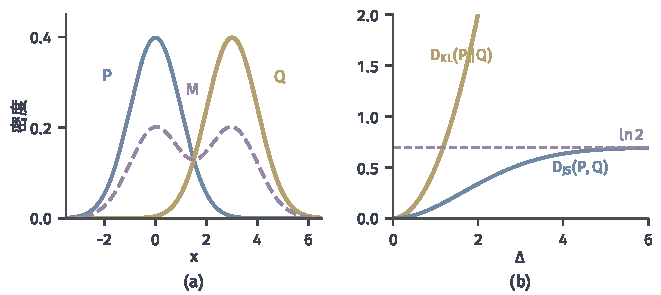
\includegraphics[width=112mm]{figures/07-probability/04-distribution-analysis/matplotlib/dcomp-js-saturation/figure.pdf}
 \caption{JS散度的饱和。(a)$P=\mathcal{N}(0,1)$（蓝）、$Q=\mathcal{N}(3,1)$（黄）与平均分布$M$（紫色虚线）。(b)$D_{\mathrm{KL}}(P\Vert Q)=\Delta^{2}/2$（黄）与$D_{\mathrm{JS}}(P,Q)$（蓝，数值积分），紫色虚线是上界$\ln2$；$\Delta=1,3,6$时JS散度依次约为$0.111$，$0.527$，$0.689$。}
 \label{fig:dcomp-js-saturation}
\end{BookInlineFigure}

\paragraph{距离性质}
JS散度对称、非负、零值只在两分布相同时取到，但它本身不满足三角不等式。在$\{0,1\}$上取$\delta_0$、$\delta_1$与均匀分布$U=(\tfrac12,\tfrac12)$。$\delta_0$与$\delta_1$相互奇异，JS散度取最大值$\ln2\approx0.6931$。$\delta_0$与$U$的平均是$(\tfrac34,\tfrac14)$，计算得
\[
 D_{\mathrm{JS}}(\delta_0,U)=\frac12\ln\frac43+\frac12\Bigl(\frac12\ln\frac23+\frac12\ln2\Bigr)=\frac34\ln\frac43\approx0.2158 .
\]
由对称性$D_{\mathrm{JS}}(U,\delta_1)$也约为$0.2158$，两者之和$0.4315$小于$0.6931$。可以证明$\sqrt{D_{\mathrm{JS}}}$满足三角不等式，因而是一个距离；证明需要把它写成某个Hilbert空间中两点的距离，篇幅较长。上例中$\sqrt{0.2158}\times2\approx0.929$，确实大于$\sqrt{0.6931}\approx0.833$。

\subsection{凸函数散度}
\label{sec:dcomp-f-divergence}

把前面几个量都写成“$Q$下对密度比的某个函数求平均”，会看到同一个形式。在$\{q>0\}$上记$t=p/q$，则
\[
 \frac12\lvert p-q\rvert=q\cdot\frac12\lvert t-1\rvert,\qquad p\ln\frac{p}{q}=q\cdot t\ln t,\qquad\frac12\bigl(\sqrt{p}-\sqrt{q}\bigr)^{2}=q\cdot\frac12\bigl(\sqrt{t}-1\bigr)^{2} .
\]
总变差、KL散度与平方Hellinger距离分别是$\int q\,f(p/q)\,\mathrm{d}\lambda$，$f$依次取$\tfrac12\lvert t-1\rvert$，$t\ln t$与$\tfrac12(\sqrt{t}-1)^{2}$。这三个函数都是凸函数，并且在$t=1$处为零，见图~\ref{fig:dcomp-f-generators}。

\begin{definition}[$f$散度]
\label{def:dcomp-f-divergence}
设$f:(0,\infty)\to\mathbb{R}$是凸函数，$f(1)=0$，并令$f(0)$为极限$\lim_{t\downarrow0}f(t)$，它可以是$+\infty$。若$P\ll Q$，定义
\begin{equation}
 D_f(P\Vert Q)=\mathbb{E}_{Q}\Bigl[f\Bigl(\frac{\mathrm{d}P}{\mathrm{d}Q}\Bigr)\Bigr]=\int_{\{q>0\}}q\,f\Bigl(\frac{p}{q}\Bigr)\,\mathrm{d}\lambda ,
 \label{eq:dcomp-f-def}
\end{equation}
称为$P$相对于$Q$的\term{$f$散度}（$f$-divergence），$f$称为它的生成函数。
\end{definition}

积分有意义：凸函数位于它的任何一条支撑线之上，存在常数$a,b$使$f(t)\geq a+bt$，所以$f(\mathrm{d}P/\mathrm{d}Q)$的负部不超过$\lvert a\rvert+\lvert b\rvert\,\mathrm{d}P/\mathrm{d}Q$，在$Q$下可积。非负性来自Jensen不等式：$\mathbb{E}_{Q}[\mathrm{d}P/\mathrm{d}Q]=1$，所以
\[
 D_f(P\Vert Q)\geq f\Bigl(\mathbb{E}_{Q}\Bigl[\frac{\mathrm{d}P}{\mathrm{d}Q}\Bigr]\Bigr)=f(1)=0 .
\]
凸性在这里起的作用，与Gibbs不等式中对数的凹性相同。

\paragraph{奇异质量}
$P$不绝对连续于$Q$时，$P$在$\{q=0\}$上有质量，那里的密度比相当于$t=+\infty$。从$\{q>0\}$一侧看，$q\,f(p/q)=p\cdot f(t)/t$，当$q\to0$而$p$固定时，它趋于$p\,f'(\infty)$，其中
\begin{equation}
 f'(\infty)=\lim_{t\to\infty}\frac{f(t)}{t}\in\mathbb{R}\cup\{+\infty\} .
 \label{eq:dcomp-f-slope-infinity}
\end{equation}
凸函数的$f(t)/t$在$t$大时单调，这个极限存在。据此把一般情形定义为
\begin{equation}
 D_f(P\Vert Q)=\int_{\{q>0\}}q\,f\Bigl(\frac{p}{q}\Bigr)\,\mathrm{d}\lambda+f'(\infty)\,P(q=0),
 \label{eq:dcomp-f-general}
\end{equation}
约定$0\cdot(+\infty)=0$。KL散度的$f'(\infty)=+\infty$，只要有奇异质量就是$+\infty$，与定义~\ref{def:dcomp-kl}一致。总变差与平方Hellinger距离的$f'(\infty)=\tfrac12$，奇异质量按一半计入：在$\{q=0\}$上$\tfrac12\lvert p-q\rvert$与$\tfrac12(\sqrt{p}-\sqrt{q})^{2}$都等于$\tfrac12p$，与直接用式~\eqref{eq:dcomp-tv-density}和式~\eqref{eq:dcomp-hellinger-def}计算的结果相同。

表~\ref{tab:dcomp-f-generators}列出常用的生成函数。JS散度也在其中：在$\{q>0\}$上把被积函数写成$q$乘以$t=p/q$的函数即得，$f'(\infty)=\tfrac12\ln2$对应于奇异部分每单位质量贡献$\tfrac12\ln2$。$\chi^{2}$散度$\int(p-q)^{2}/q\,\mathrm{d}\lambda$在例表上等于$0.09/0.3+0+0.09/0.4=0.525$。

\begin{BookInlineTable}
 \centering
 \caption{常用$f$散度的生成函数。}
 \label{tab:dcomp-f-generators}
 \begin{tabular}{lll}
  \toprule
  散度 & $f(t)$ & $f'(\infty)$\\
  \midrule
  $D_{\mathrm{KL}}(P\Vert Q)$ & $t\ln t$ & $+\infty$\\
  $D_{\mathrm{KL}}(Q\Vert P)$ & $-\ln t$ & $0$\\
  $d_{\mathrm{TV}}(P,Q)$ & $\tfrac12\lvert t-1\rvert$ & $\tfrac12$\\
  $d_{\mathrm{H}}^{2}(P,Q)$ & $\tfrac12(\sqrt{t}-1)^{2}$ & $\tfrac12$\\
  $D_{\mathrm{JS}}(P,Q)$ & $\tfrac12\bigl(t\ln\tfrac{2t}{1+t}+\ln\tfrac{2}{1+t}\bigr)$ & $\tfrac12\ln2$\\
  $\chi^{2}(P\Vert Q)$ & $(t-1)^{2}$ & $+\infty$\\
  \bottomrule
 \end{tabular}
\end{BookInlineTable}

\begin{BookInlineFigure}
 \centering
 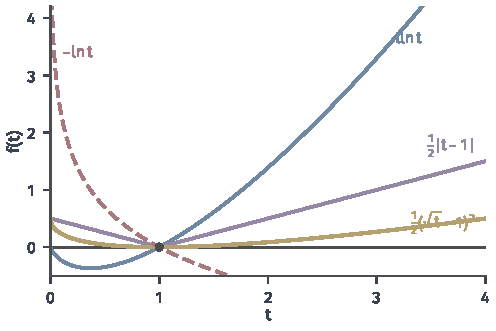
\includegraphics[width=84mm]{figures/07-probability/04-distribution-analysis/matplotlib/dcomp-f-generators/figure.pdf}
 \caption{几个生成函数在$[0,4]$上的图像：$t\ln t$（蓝，KL散度），$-\ln t$（红色虚线，反向KL散度），$\tfrac12\lvert t-1\rvert$（紫，总变差），$\tfrac12(\sqrt{t}-1)^{2}$（黄，平方Hellinger距离）。它们都是凸函数，都经过黑点$(1,0)$；右侧的斜率趋于$f'(\infty)$，决定奇异质量的计价。}
 \label{fig:dcomp-f-generators}
\end{BookInlineFigure}

表中的$-\ln t$与$t\ln t$给出两个方向的KL散度，因为在$Q$下对$-\ln(p/q)$求平均就是$D_{\mathrm{KL}}(Q\Vert P)$。一般地，$t\,f(1/t)$也是凸函数，它生成的散度是$D_f(Q\Vert P)$。生成函数也不唯一：$f(t)$与$f(t)+c(t-1)$给出同一个散度，因为附加项的贡献是$c\bigl(P(q>0)-Q(q>0)\bigr)+c\,P(q=0)=0$。

\paragraph{随机后处理}
设观测值$x$先经过一个随机处理再交给我们：给定$x$，按分布$K(x,\cdot)$产生新的结果$y$。这里$K$是第~\ref{chap:conditional-distributions}章的概率核，可以是确定的映射（$K(x,\cdot)=\delta_{T(x)}$），也可以是加噪声、四舍五入、合并类别。若原来的结果服从$P$，处理后的结果服从
\begin{equation}
 PK(B)=\int K(x,B)\,P(\mathrm{d}x),\qquad B\in\mathcal{F}_{\mathcal{Y}} .
 \label{eq:dcomp-kernel-push}
\end{equation}
直觉上，处理不会凭空增加区分$P$与$Q$的能力：任何能从$y$做出的判断，都可以先自己生成$y$再从$x$做出。下面的定理把这个直觉写成不等式。

\begin{theorem}[后处理不增加$f$散度]
\label{thm:dcomp-data-processing}
设$K$是从$\mathcal{X}$到$\mathcal{Y}$的概率核，$f$满足定义~\ref{def:dcomp-f-divergence}的条件。则
\begin{equation}
 D_f(PK\Vert QK)\leq D_f(P\Vert Q) .
 \label{eq:dcomp-data-processing}
\end{equation}
\end{theorem}

\begin{proof}
下面对$P\ll Q$的情形给出证明，这已经包含了KL散度取有限值的全部情形。若$D_f(P\Vert Q)=+\infty$，结论成立，所以设它有限。记$r=\mathrm{d}P/\mathrm{d}Q$。在一个概率空间上构造$(X,Y)$，使$X\sim Q$，给定$X=x$时$Y$的条件分布是$K(x,\cdot)$，于是$Y\sim QK$。

先找出$PK$相对于$QK$的密度。对$B\in\mathcal{F}_{\mathcal{Y}}$，由式~\eqref{eq:dcomp-kernel-push}与$r$的定义，再对$X$取条件，
\[
 PK(B)=\mathbb{E}\bigl[r(X)K(X,B)\bigr]=\mathbb{E}\bigl[r(X)\mathbf{1}_{\{Y\in B\}}\bigr]=\mathbb{E}\bigl[s(Y)\mathbf{1}_{\{Y\in B\}}\bigr],
\]
其中$s(Y)=\mathbb{E}[r(X)\mid Y]$，最后一步是条件期望的定义；$s$是可测函数，由第~\ref{chap:conditional-expectation}章，条件期望可以写成$Y$的函数。上式说明$PK\ll QK$，并且$s$就是$\mathrm{d}(PK)/\mathrm{d}(QK)$。

于是左边的散度是$\mathbb{E}[f(s(Y))]$。对凸函数$f$用条件Jensen不等式，再用全期望公式，
\[
 \mathbb{E}\bigl[f(\mathbb{E}[r(X)\mid Y])\bigr]\leq\mathbb{E}\bigl[\mathbb{E}[f(r(X))\mid Y]\bigr]=\mathbb{E}\bigl[f(r(X))\bigr]=D_f(P\Vert Q) .
\]
第~\ref{chap:conditional-expectation}章的条件Jensen不等式对定义在$\mathbb{R}$上的凸函数陈述；$f$定义在$[0,\infty)$上，$r\geq0$，证明只用到可数条支撑线，对这里的$f$同样成立。$f(r(X))$可积，因为$D_f(P\Vert Q)$有限且负部可积。
\end{proof}

$P$不绝对连续于$Q$的情形可以用同样的思路证明：取$\lambda=(P+Q)/2$，把两个密度$(\mathrm{d}P/\mathrm{d}\lambda,\mathrm{d}Q/\mathrm{d}\lambda)$一起作为二维随机向量，对二元凸函数$(a,b)\mapsto b\,f(a/b)$使用条件Jensen不等式。步骤与上面相同，只是要另外讨论$b=0$的边界。

证明的核心是一句话：处理后的密度比是处理前密度比的条件平均，而对凸函数先平均再作用，结果不超过先作用再平均。条件平均把不同$x$上的密度比混在一起，比值的起伏被抹平，凸函数度量的“偏离$1$的程度”只能变小。

\paragraph{合并类别}
在例表上做确定的合并。把$1$与$2$合并成一类，两份表变成$(0.6,0.4)$与$(0.3,0.7)$，KL散度从$0.2773$降到
\[
 0.6\ln\frac{0.6}{0.3}+0.4\ln\frac{0.4}{0.7}\approx0.1920 ,
\]
总变差仍是$0.3$。总变差不变，是因为合并后仍能区分最坏事件$A^{*}=\{0\}$。若改把$0$与$2$合并，两份表都变成$(0.7,0.3)$，所有散度都变成零：点$0$处$P$多出的$0.3$与点$2$处$Q$多出的$0.3$被并到同一类里，正好抵消，区分两个分布的信息全部丢失。图~\ref{fig:dcomp-merging}画出这三种情况。

\begin{BookInlineFigure}
 \centering
 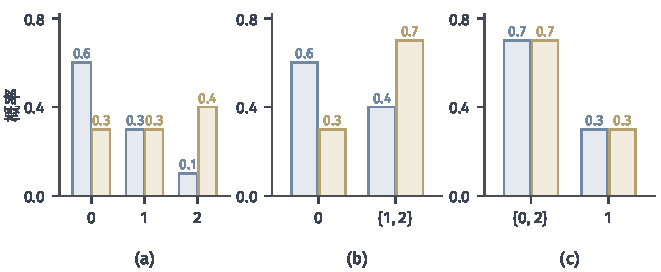
\includegraphics[width=112mm]{figures/07-probability/04-distribution-analysis/matplotlib/dcomp-merging/figure.pdf}
 \caption{确定性后处理对例表的影响，蓝色为$P$，黄色为$Q$。(a)原表：$d_{\mathrm{TV}}=0.3$，$D_{\mathrm{KL}}(P\Vert Q)\approx0.2773$。(b)合并$1$与$2$：$d_{\mathrm{TV}}=0.3$，$D_{\mathrm{KL}}\approx0.1920$。(c)合并$0$与$2$：两表相同，所有散度为零。}
 \label{fig:dcomp-merging}
\end{BookInlineFigure}

若$T$是可测的一一映射且逆映射也可测，对$T$与$T^{-1}$各用一次式~\eqref{eq:dcomp-data-processing}，得到$D_f$在$T$下不变。重新标号、单位换算这类可逆变换不改变任何$f$散度。

\subsection{Rényi散度}
\label{sec:dcomp-renyi}

KL散度按$P$的权重平均对数比。另一种做法是对密度比取幂：在$\{q>0\}$上，
\[
 \int p^{\alpha}q^{1-\alpha}\,\mathrm{d}\lambda=\mathbb{E}_{Q}\Bigl[\Bigl(\frac{p}{q}\Bigr)^{\alpha}\Bigr] .
\]
阶数$\alpha>1$时，幂函数放大大的比值，散度主要由“$P$比$Q$多出很多”的位置决定；$\alpha<1$时放大作用变弱。取对数并归一化，就得到一族以$\alpha$为参数的比较量。

\begin{definition}[Rényi散度]
\label{def:dcomp-renyi}
设$\alpha\in(0,1)\cup(1,\infty)$，$p,q$是相对于共同支配测度$\lambda$的密度。$P$相对于$Q$的$\alpha$阶\term{Rényi散度}（Rényi divergence）是
\begin{equation}
 D_{\alpha}(P\Vert Q)=\frac{1}{\alpha-1}\ln\int p^{\alpha}q^{1-\alpha}\,\mathrm{d}\lambda ,
 \label{eq:dcomp-renyi-def}
\end{equation}
其中被积函数在$p=0$处取$0$；$\alpha>1$时，在$q=0<p$处取$+\infty$。
\end{definition}

零密度的约定决定了无穷值何时出现。$\alpha>1$时，$q^{1-\alpha}$在$q\to0$时趋于无穷，只要$P(q=0)>0$，积分就是$+\infty$，散度为$+\infty$，这与KL散度要求$P\ll Q$一致。$\alpha<1$时，$q^{1-\alpha}\to0$，奇异质量对积分没有贡献；积分为$0$当且仅当$pq=0$几乎处处，即两个分布相互奇异，此时$\ln0=-\infty$除以负数$\alpha-1$，散度同样为$+\infty$。与Hellinger距离一样，被积函数关于密度一次齐次，结果与$\lambda$的选取无关。

两个特殊阶数与前面的量直接对应。$\alpha=\tfrac12$时积分是Bhattacharyya系数，$\alpha=2$时积分是$\int p^{2}/q\,\mathrm{d}\lambda$，它等于$1+\chi^{2}(P\Vert Q)$，所以
\begin{equation}
 D_{1/2}(P\Vert Q)=-2\ln B(P,Q),\qquad D_{2}(P\Vert Q)=\ln\bigl(1+\chi^{2}(P\Vert Q)\bigr) .
 \label{eq:dcomp-renyi-special}
\end{equation}
在例表上，由$B\approx0.9243$与$\chi^{2}=0.525$，
\[
 D_{1/2}\approx0.1575,\qquad D_{\mathrm{KL}}\approx0.2773,\qquad D_{2}=\ln1.525\approx0.4220 .
\]
KL散度恰好夹在中间。图~\ref{fig:dcomp-renyi-order}画出$D_{\alpha}$随$\alpha$的变化，它是一条单调上升的曲线，在$\alpha=1$处连续地经过KL散度。

\begin{BookInlineFigure}
 \centering
 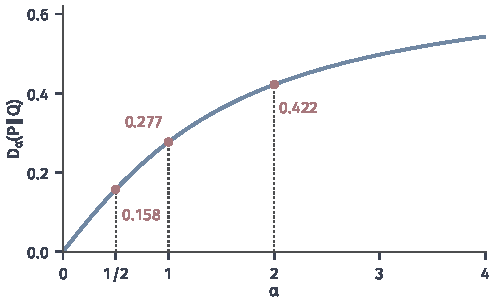
\includegraphics[width=84mm]{figures/07-probability/04-distribution-analysis/matplotlib/dcomp-renyi-order/figure.pdf}
 \caption{例表的Rényi散度$D_{\alpha}(P\Vert Q)$随阶数$\alpha$的变化（蓝）。红点依次是$\alpha=\tfrac12$处的$-2\ln B\approx0.158$，$\alpha=1$处的KL散度$0.4\ln2\approx0.277$，$\alpha=2$处的$\ln(1+\chi^{2})\approx0.422$。}
 \label{fig:dcomp-renyi-order}
\end{BookInlineFigure}

\begin{theorem}[阶数的单调性与KL极限]
\label{thm:dcomp-renyi-order}
对$0<\alpha<1<\beta$，
\begin{equation}
 D_{\alpha}(P\Vert Q)\leq D_{\mathrm{KL}}(P\Vert Q)\leq D_{\beta}(P\Vert Q),
 \label{eq:dcomp-renyi-sandwich}
\end{equation}
并且$\alpha\mapsto D_{\alpha}(P\Vert Q)$在$(0,1)$与$(1,\infty)$上都单调不减，$\alpha\uparrow1$时$D_{\alpha}(P\Vert Q)\to D_{\mathrm{KL}}(P\Vert Q)$。
\end{theorem}

\begin{proof}
若$P$不绝对连续于$Q$，则$D_{\mathrm{KL}}$与所有$\beta>1$的$D_{\beta}$都是$+\infty$，不等式与右侧的单调性成立；左侧的论证不用绝对连续，放在下面一并处理。先设$P\ll Q$。

\emph{改写成幂平均。}在$\{p>0\}$上令$R=q/p$，它在$P$下几乎处处取正的有限值。被积函数在$p=0$处为零，所以
\[
 \int p^{\alpha}q^{1-\alpha}\,\mathrm{d}\lambda=\int_{\{p>0\}}p\,R^{1-\alpha}\,\mathrm{d}\lambda=\mathbb{E}_{P}\bigl[R^{s}\bigr],\qquad s=1-\alpha .
\]
对$s\neq0$记$M_s=(\mathbb{E}_{P}[R^{s}])^{1/s}$，称为$R$的$s$次幂平均，再记$M_0=\exp(\mathbb{E}_{P}[\ln R])$。由式~\eqref{eq:dcomp-renyi-def}与式~\eqref{eq:dcomp-kl-def}，
\[
 D_{\alpha}(P\Vert Q)=-\ln M_{1-\alpha},\qquad D_{\mathrm{KL}}(P\Vert Q)=-\mathbb{E}_{P}[\ln R]=-\ln M_0 .
\]
$\alpha$增大时$s$减小，所以只需证明$M_s$关于$s$单调不减。

\emph{幂平均的单调性。}对$0<s<t$，函数$u\mapsto u^{t/s}$在$[0,\infty)$上凸，由Jensen不等式，
\[
 \bigl(\mathbb{E}_{P}[R^{s}]\bigr)^{t/s}\leq\mathbb{E}_{P}[R^{t}],
\]
开$t$次方得$M_s\leq M_t$。对$s<t<0$，把同一结论用于$1/R$与指数$-t<-s$，取倒数即得。对$s<0<t$，由对数的凹性，
\[
 t\,\mathbb{E}_{P}[\ln R]\leq\ln\mathbb{E}_{P}[R^{t}],\qquad s\,\mathbb{E}_{P}[\ln R]\leq\ln\mathbb{E}_{P}[R^{s}] .
\]
第一式除以$t>0$得$\ln M_0\leq\ln M_t$；第二式除以$s<0$，不等号反向，得$\ln M_0\geq\ln M_s$。于是$M_s\leq M_0\leq M_t$，这就是式~\eqref{eq:dcomp-renyi-sandwich}与两段上的单调性。$\mathbb{E}_{P}[R^{s}]=+\infty$（$s<0$时可能发生）时$M_s=0$，对应的散度为$+\infty$，不等式仍成立。

\emph{左侧的极限。}令$\alpha\uparrow1$，即$s\downarrow0$。对固定的$R>0$，$s\mapsto R^{s}$是凸函数，差商$(R^{s}-1)/s$随$s$减小而单调下降，极限是$\ln R$；$s=1$时差商为$R-1$，在$P$下可积。由单调收敛定理（单调下降、首项可积），
\[
 a_s=\mathbb{E}_{P}\Bigl[\frac{R^{s}-1}{s}\Bigr]\downarrow\mathbb{E}_{P}[\ln R]=-D_{\mathrm{KL}}(P\Vert Q) .
\]
而$\mathbb{E}_{P}[R^{s}]=1+s\,a_s$，所以
\[
 -D_{\alpha}(P\Vert Q)=\frac{1}{s}\ln\mathbb{E}_{P}[R^{s}]=\frac{\ln(1+s\,a_s)}{s} .
\]
若$D_{\mathrm{KL}}$有限，$s\,a_s\to0$，$\ln(1+u)/u\to1$，所以$-D_{\alpha}\to-D_{\mathrm{KL}}$。若$D_{\mathrm{KL}}=+\infty$，由$\ln(1+u)\leq u$得$-D_{\alpha}\leq a_s\to-\infty$。两种情形都有$D_{\alpha}\to D_{\mathrm{KL}}$。

最后，$P$不绝对连续于$Q$时，把$R$在$\{q=0<p\}$上定义为$0$，上面关于$s\in(0,1)$的改写和左侧的极限论证照样成立，结论是$D_{\alpha}\to+\infty=D_{\mathrm{KL}}$。
\end{proof}

\paragraph{另一侧的极限需要条件}
$\alpha\downarrow1$时，$D_{\beta}$未必趋于KL散度。在正整数上取
\[
 p_k=c\,k^{-3},\qquad q_k=(\mathrm{e}-1)\,\mathrm{e}^{-k},\qquad k=1,2,\dots,
\]
其中$c=1/\sum_kk^{-3}\approx0.8319$。对数比$\ln(p_k/q_k)$约按$k$线性增长，而$p_k$按$k^{-3}$衰减，所以$D_{\mathrm{KL}}(P\Vert Q)=\sum_kp_k\ln(p_k/q_k)$收敛，数值约为$0.1446$。但对任何$\beta>1$，
\[
 p_k^{\beta}q_k^{1-\beta}=c^{\beta}(\mathrm{e}-1)^{1-\beta}\,k^{-3\beta}\,\mathrm{e}^{(\beta-1)k}\to+\infty,
\]
级数发散，$D_{\beta}(P\Vert Q)=+\infty$。比值$p_k/q_k$的增长是指数型的，任何正次幂都会让它压过$p_k$的多项式衰减，而对数只把它变成线性增长。若存在某个$\beta>1$使$D_{\beta}$有限，那么$\alpha\downarrow1$时$D_{\alpha}\to D_{\mathrm{KL}}$，证明与上面类似，用支配收敛定理代替单调收敛定理。

\paragraph{与$f$散度的关系}
令$f_{\alpha}(t)=(t^{\alpha}-1)/(\alpha-1)$。$\alpha>1$时$t^{\alpha}$凸，除以正数；$\alpha<1$时$t^{\alpha}$凹，除以负数，所以$f_{\alpha}$总是凸函数，并且$f_{\alpha}(1)=0$。它生成的$f$散度记作$H_{\alpha}$，对比式~\eqref{eq:dcomp-renyi-def}，
\[
 D_{\alpha}(P\Vert Q)=\frac{1}{\alpha-1}\ln\bigl(1+(\alpha-1)H_{\alpha}(P\Vert Q)\bigr) .
\]
右边是$H_{\alpha}$的单调增函数，所以定理~\ref{thm:dcomp-data-processing}立即给出：后处理也不增加Rényi散度。

单调变换保住了大小顺序，却改变了结构，$D_{\alpha}$本身一般不是$f$散度。任何$f$散度在不交区域上按权相加：若$P=\tfrac12P_1+\tfrac12P_2$，$Q=\tfrac12Q_1+\tfrac12Q_2$，并且$P_1,Q_1$集中在$A$上，$P_2,Q_2$集中在$A^{\mathrm{c}}$上，把式~\eqref{eq:dcomp-f-general}的积分拆到$A$与$A^{\mathrm{c}}$上就得到
\[
 D_f(P\Vert Q)=\tfrac12D_f(P_1\Vert Q_1)+\tfrac12D_f(P_2\Vert Q_2) .
\]
在$\{0,1,2\}$上取$A=\{0,1\}$与
\[
 P=(\tfrac12,\ 0,\ \tfrac12),\qquad Q=(\tfrac14,\ \tfrac14,\ \tfrac12) .
\]
按上面的分解，$P_1=(1,0)$与$Q_1=(\tfrac12,\tfrac12)$在$A$上，$P_2,Q_2$都是$\delta_2$。直接计算，
\[
 D_2(P\Vert Q)=\ln\Bigl(\frac{1/4}{1/4}+\frac{1/4}{1/2}\Bigr)=\ln1.5\approx0.4055,
\]
而按块加权的结果是
\[
 \tfrac12D_2(P_1\Vert Q_1)+\tfrac12D_2(P_2\Vert Q_2)=\tfrac12\ln2+0\approx0.3466 .
\]
两者不等，所以不存在$f$使$D_2=D_f$对所有分布对成立。作为对照，KL散度满足这个可加性：$D_{\mathrm{KL}}(P\Vert Q)$与$\tfrac12D_{\mathrm{KL}}(P_1\Vert Q_1)$都等于$\tfrac12\ln2$。

\section{基于测试函数的比较}
\label{sec:dcomp-ipm}

密度比较要求两个分布写在同一个支配测度下，并且只看同一位置上的取值。另一种做法不碰密度，只看两个分布对一些函数给出的平均。选定一个函数$g$，读出$\mathbb{E}_{P}[g]$与$\mathbb{E}_{Q}[g]$，两者的差就是用$g$这把“尺子”量到的差异。用一族尺子同时去量，取最大的读数差，就得到一个比较量。式~\eqref{eq:dcomp-tv-dual}已经是这种形式：总变差是有界函数单位球上的最大期望差。这里要回答的是：换成别的函数类会得到什么，函数类要多丰富才能分辨所有不同的分布，以及怎样实际算出上确界。

\subsection{函数类与可辨别差异}
\label{sec:dcomp-ipm-classes}

\begin{definition}[积分概率度量]
\label{def:dcomp-ipm}
设$\mathcal{G}$是一族$\mathcal{X}$上的实值可测函数，其中每个$g$在$P$与$Q$下都可积。称
\begin{equation}
 d_{\mathcal{G}}(P,Q)=\sup_{g\in\mathcal{G}}\bigl\lvert\mathbb{E}_{P}[g]-\mathbb{E}_{Q}[g]\bigr\rvert
 \label{eq:dcomp-ipm-def}
\end{equation}
为由$\mathcal{G}$生成的\term{积分概率度量}（integral probability metric）。
\end{definition}

这个量对称，并且满足三角不等式：对第三个分布$R$与每个$g$，
\[
 \lvert\mathbb{E}_{P}g-\mathbb{E}_{R}g\rvert\leq\lvert\mathbb{E}_{P}g-\mathbb{E}_{Q}g\rvert+\lvert\mathbb{E}_{Q}g-\mathbb{E}_{R}g\rvert ,
\]
再对$g$取上确界。定义要检查两件事。

第一，上确界是否有限。若$\mathcal{G}$对数乘封闭，例如取全体有界可测函数而不限制大小，只要某个$g$的读数差不为零，把$g$放大$c$倍读数差就放大$c$倍，上确界是$+\infty$。所以函数类通常要带一个范数约束，如$\lVert g\rVert_{\infty}\leq1$。

第二，零值能否辨别分布。比较量为零只说明$P$与$Q$在$\mathcal{G}$中每个函数上的平均相同。若$\mathcal{G}$太小，不同的分布也可能得到零。取$\mathcal{G}$只含$x$与$x^{2}$两个函数，它只比较均值与二阶矩。标准高斯分布$P$与区间$(-\sqrt3,\sqrt3)$上的均匀分布$Q$的均值都是$0$，二阶矩都是$1$，所以这个函数类给出的比较量为零，两个分布却明显不同，见图~\ref{fig:dcomp-moment-matching}。一旦加入$\cos x$或$\mathbf{1}_{\{\lvert x\rvert\leq1\}}$这样的函数，差异立即显现：
\[
 \mathbb{E}_{P}[\cos X]-\mathbb{E}_{Q}[\cos X]=\mathrm{e}^{-1/2}-\frac{\sin\sqrt3}{\sqrt3}\approx0.0367,
\]
\[
 P(\lvert X\rvert\leq1)-Q(\lvert X\rvert\leq1)=\bigl(2\Phi(1)-1\bigr)-\frac{1}{\sqrt3}\approx0.1053 .
\]

\begin{BookInlineFigure}
 \centering
 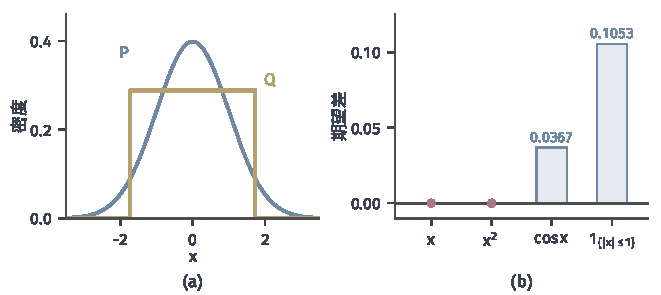
\includegraphics[width=112mm]{figures/07-probability/04-distribution-analysis/matplotlib/dcomp-moment-matching/figure.pdf}
 \caption{函数类决定能看到的差异。(a)$P=\mathcal{N}(0,1)$（蓝）与$Q=\operatorname{Unif}(-\sqrt3,\sqrt3)$（黄），均值都是$0$，方差都是$1$。(b)四个测试函数上的期望差$\mathbb{E}_{P}[g]-\mathbb{E}_{Q}[g]$：$x$与$x^{2}$为零（红点），$\cos x$与$\mathbf{1}_{\{\lvert x\rvert\leq1\}}$不为零。}
 \label{fig:dcomp-moment-matching}
\end{BookInlineFigure}

几种常见的函数类各有含义。有界函数单位球给出$2d_{\mathrm{TV}}$，能辨别任何两个不同的分布，但对位置的微小移动同样“看得见”，见第~\ref{sec:dcomp-tv-definition}节末尾。$\mathbb{R}$上半直线的示性函数$\mathbf{1}_{(-\infty,t]}$给出$\sup_t\lvert F_P(t)-F_Q(t)\rvert$，称为\term{Kolmogorov距离}（Kolmogorov distance）；分布函数决定分布，所以它也能辨别分布。$\mathbb{R}^{d}$上的全体有界连续函数也能辨别分布，这是第~\ref{chap:weak-convergence-of-distributions}章中弱收敛极限唯一的依据。1-Lipschitz函数类给出第~\ref{sec:dcomp-wasserstein}节的一阶Wasserstein距离。

函数类越大，比较越严格，但上确界也越难计算：对一般的函数类，要在无穷维集合上求最大值。下面构造一类函数，使上确界有闭式解。

\subsection{核均值}
\label{sec:dcomp-kernel-mean}

取再生核Hilbert空间（RKHS）的单位球作为函数类。设$k$是$\mathcal{X}$上的正定核，$\mathcal{H}$是它的RKHS，内积记作$\langle\cdot,\cdot\rangle_{\mathcal{H}}$。卷四给出了它的基本性质：每个$x$对应一个函数$k(x,\cdot)\in\mathcal{H}$，并且对一切$g\in\mathcal{H}$，
\begin{equation}
 g(x)=\bigl\langle g,\,k(x,\cdot)\bigr\rangle_{\mathcal{H}},\qquad\bigl\lVert k(x,\cdot)\bigr\rVert_{\mathcal{H}}=\sqrt{k(x,x)},
 \label{eq:dcomp-reproducing}
\end{equation}
可参考\BookChapterRef{chap:rkhs}{卷四第23章“再生核Hilbert空间”}。映射$x\mapsto k(x,\cdot)$是特征映射，它把$\mathcal{X}$中的点放进Hilbert空间。为避免与概率核混淆，本节的核用小写$k$。

再生性质~\eqref{eq:dcomp-reproducing}把求值变成内积。若在两边对$X\sim P$取期望，并把期望移进内积里，就得到
\[
 \mathbb{E}_{P}[g(X)]=\bigl\langle g,\ \mathbb{E}_{P}[k(X,\cdot)]\bigr\rangle_{\mathcal{H}} .
\]
右边的$\mathbb{E}_{P}[k(X,\cdot)]$是特征点的平均位置，也就是把单位质量按$P$放到这些特征点上之后的重心。下面的定理说明这个重心在什么条件下存在，并绕开“向量值期望”的定义，直接用内积刻画它。

\begin{theorem}[核均值]
\label{thm:dcomp-kernel-mean}
设$\mathcal{H}$可分，特征映射$x\mapsto k(x,\cdot)$可测，并且
\begin{equation}
 \mathbb{E}_{P}\Bigl[\sqrt{k(X,X)}\Bigr]<\infty .
 \label{eq:dcomp-kernel-moment}
\end{equation}
则每个$g\in\mathcal{H}$在$P$下可积，并且存在唯一的$m_P\in\mathcal{H}$，使
\begin{equation}
 \mathbb{E}_{P}[g(X)]=\langle g,m_P\rangle_{\mathcal{H}},\qquad g\in\mathcal{H} .
 \label{eq:dcomp-kernel-mean}
\end{equation}
它的取值是$m_P(y)=\mathbb{E}_{P}[k(X,y)]$。
\end{theorem}

\begin{proof}
对$g\in\mathcal{H}$，$g(x)=\langle g,k(x,\cdot)\rangle_{\mathcal{H}}$是连续线性泛函与可测映射的复合，所以$g$可测。由Cauchy--Schwarz不等式与式~\eqref{eq:dcomp-reproducing}，
\[
 \lvert g(x)\rvert\leq\lVert g\rVert_{\mathcal{H}}\sqrt{k(x,x)} .
\]
由条件~\eqref{eq:dcomp-kernel-moment}，$g$在$P$下可积，并且线性泛函$L(g)=\mathbb{E}_{P}[g(X)]$满足
\[
 \lvert L(g)\rvert\leq\mathbb{E}_{P}\Bigl[\sqrt{k(X,X)}\Bigr]\,\lVert g\rVert_{\mathcal{H}},
\]
是有界线性泛函。由Riesz表示定理，存在唯一的$m_P\in\mathcal{H}$使$L(g)=\langle g,m_P\rangle_{\mathcal{H}}$，可参考\BookChapterRef{chap:function-inner-product-spaces}{卷四第12章“内积空间”}。取$g=k(y,\cdot)$，由式~\eqref{eq:dcomp-reproducing}，左边是$\mathbb{E}_{P}[k(X,y)]$，右边是$m_P(y)$。
\end{proof}

$m_P$称为$P$的\term{核均值}（kernel mean embedding），映射$P\mapsto m_P$把概率分布表示为$\mathcal{H}$中的元素。可分性在这里的作用是保证可测性在两种意义下一致：可分Hilbert空间中，“每个$g(x)=\langle g,k(x,\cdot)\rangle$都可测”与“特征映射作为Hilbert空间值映射可测”是等价的，所以定理的条件可以按任一种理解检查。条件~\eqref{eq:dcomp-kernel-moment}是特征点到原点距离的一阶矩，有界核（如高斯核，$k(x,x)=1$）对任何分布都满足它。这一节新增的只是“分布的表示”，RKHS本身仍是卷四的对象。

\paragraph{例表上的核均值}
在例表上取$\sigma=1$的高斯核$k(x,y)=\exp(-(x-y)^{2}/2)$。分布有限时期望就是加权和，
\[
 m_P=\sum_{i}p_i\,k(x_i,\cdot)=0.6\,k(0,\cdot)+0.3\,k(1,\cdot)+0.1\,k(2,\cdot) .
\]
它是三个以$0,1,2$为中心的高斯隆起按概率加权之和，见图~\ref{fig:dcomp-kernel-mean}(a)中的点线。在三个支撑点上，
\[
 m_P(0)\approx0.7955,\qquad m_P(1)\approx0.7246,\qquad m_P(2)\approx0.3632,
\]
\[
 m_Q(0)\approx0.5361,\qquad m_Q(1)\approx0.7246,\qquad m_Q(2)\approx0.6226 .
\]
核均值是概率质量用核“抹开”后的形状。$P$的质量偏左，$m_P$的峰也偏左。

\subsection{MMD}
\label{sec:dcomp-mmd}

有了核均值，RKHS单位球上的最大期望差就是一个Hilbert空间中的最大内积问题，答案由Cauchy--Schwarz不等式直接给出。

\begin{theorem}[MMD的表示]
\label{thm:dcomp-mmd}
设$P,Q$都满足条件~\eqref{eq:dcomp-kernel-moment}。则
\begin{equation}
 \operatorname{MMD}_k(P,Q)=\sup_{\lVert g\rVert_{\mathcal{H}}\leq1}\bigl\lvert\mathbb{E}_{P}[g]-\mathbb{E}_{Q}[g]\bigr\rvert=\lVert m_P-m_Q\rVert_{\mathcal{H}} .
 \label{eq:dcomp-mmd-def}
\end{equation}
设$X,X'\sim P$，$Y,Y'\sim Q$，四者相互独立，则
\begin{equation}
 \operatorname{MMD}_k^{2}(P,Q)=\mathbb{E}\bigl[k(X,X')\bigr]-2\,\mathbb{E}\bigl[k(X,Y)\bigr]+\mathbb{E}\bigl[k(Y,Y')\bigr] .
 \label{eq:dcomp-mmd-kernel}
\end{equation}
\end{theorem}

\begin{proof}
由式~\eqref{eq:dcomp-kernel-mean}，
\[
 \mathbb{E}_{P}[g]-\mathbb{E}_{Q}[g]=\langle g,m_P-m_Q\rangle_{\mathcal{H}} .
\]
由Cauchy--Schwarz不等式，单位球上它的绝对值不超过$\lVert m_P-m_Q\rVert_{\mathcal{H}}$；若$m_P\neq m_Q$，取$m_P-m_Q$方向上的单位向量$g^{*}$即可达到，若相等则两边都是零。这证明了式~\eqref{eq:dcomp-mmd-def}。

展开平方范数，
\[
 \lVert m_P-m_Q\rVert_{\mathcal{H}}^{2}=\langle m_P,m_P\rangle_{\mathcal{H}}-2\langle m_P,m_Q\rangle_{\mathcal{H}}+\langle m_Q,m_Q\rangle_{\mathcal{H}} .
\]
对中间一项，把式~\eqref{eq:dcomp-kernel-mean}用于$g=m_P$与分布$Q$，再用$m_P(y)=\mathbb{E}_{P}[k(X,y)]$，
\[
 \langle m_P,m_Q\rangle_{\mathcal{H}}=\mathbb{E}_{Q}\bigl[m_P(Y)\bigr]=\mathbb{E}\bigl[k(X,Y)\bigr] .
\]
最后一步是对独立的$(X,Y)$用Fubini定理，所需的可积性来自$\lvert k(x,y)\rvert\leq\sqrt{k(x,x)k(y,y)}$与条件~\eqref{eq:dcomp-kernel-moment}。另两项同理。
\end{proof}

\term{最大均值差异}（maximum mean discrepancy）这个名字来自式~\eqref{eq:dcomp-mmd-def}的左端，简称MMD。达到上确界的$g^{*}$称为\term{见证函数}（witness function），它在$P$质量多于$Q$的地方取正值，在少于$Q$的地方取负值，是RKHS单位球中最能“看出”两者差别的那把尺子。式~\eqref{eq:dcomp-mmd-kernel}把无穷维的上确界化成了三个核期望：同一分布内两点的平均相似度，减去跨分布两点的平均相似度的两倍。

\paragraph{例表上的计算}
继续用$\sigma=1$的高斯核。记$\bm{K}$为$3\times3$矩阵，$\bm{K}_{i,j}=k(i-1,j-1)$，即$\exp(-(i-j)^{2}/2)$。三个核期望是二次型，
\[
 \bm{p}^{\top}\bm{K}\bm{p}\approx0.7310,\qquad\bm{p}^{\top}\bm{K}\bm{q}\approx0.6013,\qquad\bm{q}^{\top}\bm{K}\bm{q}\approx0.6272 .
\]
由式~\eqref{eq:dcomp-mmd-kernel}，
\[
 \operatorname{MMD}_k^{2}(P,Q)\approx0.7310-2\times0.6013+0.6272=0.1556 .
\]
也可以直接用$\bm{p}-\bm{q}=(0.3,0,-0.3)^{\top}$计算二次型：
\[
 (\bm{p}-\bm{q})^{\top}\bm{K}(\bm{p}-\bm{q})=0.09\,(1+1-2\mathrm{e}^{-2})=0.18(1-\mathrm{e}^{-2})\approx0.1556 .
\]
开方得$\operatorname{MMD}_k(P,Q)\approx0.3945$。见证函数在三个支撑点上的值是$0.6575$，$0$，$-0.6575$，代入
\[
 \begin{aligned}
 \mathbb{E}_{P}[g^{*}]-\mathbb{E}_{Q}[g^{*}]&=\sum_i(p_i-q_i)\,g^{*}(x_i)\\
 &=0.3\times0.6575+(-0.3)\times(-0.6575)\approx0.3945 ,
 \end{aligned}
\]
与MMD相等，见图~\ref{fig:dcomp-kernel-mean}(b)。

\begin{BookInlineFigure}
 \centering
 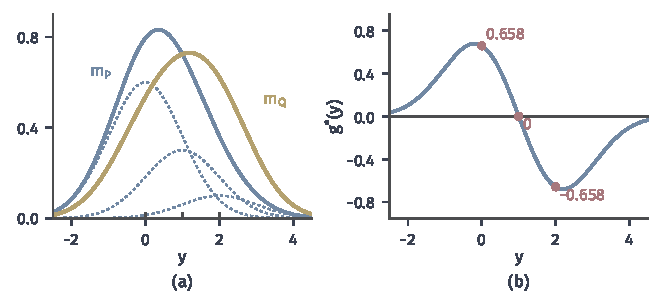
\includegraphics[width=112mm]{figures/07-probability/04-distribution-analysis/matplotlib/dcomp-kernel-mean/figure.pdf}
 \caption{例表的核均值，高斯核$\sigma=1$。(a)$m_P$（蓝）与$m_Q$（黄）；蓝色点线是三个加权核截面$p_i\,k(x_i,\cdot)$，深灰短线标出支撑点$0,1,2$。(b)见证函数$g^{*}=(m_P-m_Q)/\operatorname{MMD}_k$，红点是它在支撑点上的值。}
 \label{fig:dcomp-kernel-mean}
\end{BookInlineFigure}

式~\eqref{eq:dcomp-mmd-kernel}是两个总体分布之间的量。实际中常常只有两组样本，把期望换成样本平均就得到估计值；估计的偏差、方差与检验属于卷八的内容，这里只讨论总体量本身。

\subsection{核的辨别能力}
\label{sec:dcomp-characteristic}

MMD为零意味着$m_P=m_Q$。核均值是否把不同的分布映到不同的元素，取决于核。

\begin{definition}[特征核]
\label{def:dcomp-characteristic}
设$\mathcal{P}_k$是满足条件~\eqref{eq:dcomp-kernel-moment}的全体概率分布。若映射$P\mapsto m_P$在$\mathcal{P}_k$上是单射，则称$k$为\term{特征核}（characteristic kernel）。
\end{definition}

由式~\eqref{eq:dcomp-mmd-def}，$k$是特征核当且仅当对$\mathcal{P}_k$中的分布，$\operatorname{MMD}_k(P,Q)=0$等价于$P=Q$。不是特征核的例子很容易造。线性核$k(x,y)=xy$的RKHS只含线性函数，$m_P(y)=y\,\mathbb{E}_{P}[X]$，MMD只比较均值。二次核$k(x,y)=(1+xy)^{2}$的核均值是
\[
 m_P(y)=\mathbb{E}_{P}\bigl[(1+Xy)^{2}\bigr]=1+2y\,\mathbb{E}_{P}[X]+y^{2}\,\mathbb{E}_{P}[X^{2}],
\]
它只记录前两阶矩。图~\ref{fig:dcomp-moment-matching}中的两个分布在这个核下MMD为零。高斯核则不同。

在$\mathbb{R}^{d}$上取带宽$\sigma>0$的高斯核
\begin{equation}
 k_\sigma(\bm{x},\bm{y})=\exp\Bigl(-\frac{\lVert\bm{x}-\bm{y}\rVert_2^{2}}{2\sigma^{2}}\Bigr) .
 \label{eq:dcomp-gauss-kernel}
\end{equation}
它的谱表示把MMD与特征函数联系起来。

\begin{theorem}[高斯核的谱表示]
\label{thm:dcomp-gauss-characteristic}
设$k_\sigma$如式~\eqref{eq:dcomp-gauss-kernel}，$\Lambda_\sigma$是协方差矩阵为$\sigma^{-2}\bm{I}$的中心高斯分布。对$\mathbb{R}^{d}$上任意概率分布$P,Q$，
\begin{equation}
 \operatorname{MMD}_{k_\sigma}^{2}(P,Q)=\int_{\mathbb{R}^{d}}\bigl\lvert\phi_P(\bm{\omega})-\phi_Q(\bm{\omega})\bigr\rvert^{2}\,\Lambda_\sigma(\mathrm{d}\bm{\omega}),
 \label{eq:dcomp-mmd-spectral}
\end{equation}
其中$\phi_P,\phi_Q$是两个分布的特征函数。因此$k_\sigma$是特征核。
\end{theorem}

\begin{proof}
设$\bm{W}\sim\Lambda_\sigma$。高斯分布的特征函数给出，对任意$\bm{u}\in\mathbb{R}^{d}$，
\[
 \mathbb{E}\bigl[\mathrm{e}^{\mathrm{i}\langle\bm{W},\bm{u}\rangle}\bigr]=\exp\Bigl(-\frac{\lVert\bm{u}\rVert_2^{2}}{2\sigma^{2}}\Bigr)=k_\sigma(\bm{x},\bm{y}),\qquad\bm{u}=\bm{x}-\bm{y} .
\]
取$\bm{X}\sim P$，$\bm{Y}\sim Q$与$\bm{W}$相互独立。被积函数的模为$1$，由Fubini定理可以先对$\bm{X},\bm{Y}$积分：
\[
 \mathbb{E}\bigl[k_\sigma(\bm{X},\bm{Y})\bigr]=\mathbb{E}\Bigl[\mathbb{E}\bigl[\mathrm{e}^{\mathrm{i}\langle\bm{W},\bm{X}\rangle}\bigr]\,\overline{\mathbb{E}\bigl[\mathrm{e}^{\mathrm{i}\langle\bm{W},\bm{Y}\rangle}\bigr]}\Bigm|\bm{W}\Bigr]=\int\phi_P(\bm{\omega})\overline{\phi_Q(\bm{\omega})}\,\Lambda_\sigma(\mathrm{d}\bm{\omega}) .
\]
对$(P,P)$与$(Q,Q)$同样计算，代入式~\eqref{eq:dcomp-mmd-kernel}，三项合成$\lvert\phi_P-\phi_Q\rvert^{2}$的积分，即式~\eqref{eq:dcomp-mmd-spectral}。高斯核有界，条件~\eqref{eq:dcomp-kernel-moment}对任何分布成立。

若MMD为零，则$\phi_P=\phi_Q$在$\Lambda_\sigma$几乎处处成立。$\Lambda_\sigma$有处处为正的密度，两个连续函数在一个满测度集上相等，这个集合在$\mathbb{R}^{d}$中稠密，所以它们处处相等。由第~\ref{chap:weak-convergence-of-distributions}章特征函数的唯一性，$P=Q$。
\end{proof}

式~\eqref{eq:dcomp-mmd-spectral}说明高斯核MMD是特征函数之差在各频率上的加权平方和，权重是方差为$\sigma^{-2}$的高斯分布。带宽$\sigma$越大，权重越集中在低频。图~\ref{fig:dcomp-mmd-spectrum}比较$\mathcal{N}(0,1)$与$\operatorname{Unif}(-\sqrt3,\sqrt3)$：两者的特征函数在$\omega=0$附近按前两阶矩展开后相同，差异$\lvert\phi_P-\phi_Q\rvert^{2}$在$\omega\approx2.4$处最大。$\sigma=2$的权重在那里几乎为零，MMD只有约$0.0174$；$\sigma=0.5$的权重覆盖了这一频段，MMD约为$0.1329$。三个带宽都给出正值，因为高斯权重处处为正，任何频段上的差异都会被计入；但数值大小强烈依赖于带宽，不同核下的MMD不能直接比较。

\begin{BookInlineFigure}
 \centering
 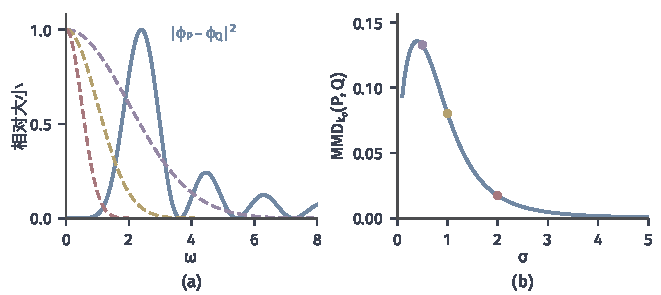
\includegraphics[width=112mm]{figures/07-probability/04-distribution-analysis/matplotlib/dcomp-mmd-spectrum/figure.pdf}
 \caption{高斯核MMD的频率图景，$P=\mathcal{N}(0,1)$，$Q=\operatorname{Unif}(-\sqrt3,\sqrt3)$。(a)蓝线是$\lvert\phi_P(\omega)-\phi_Q(\omega)\rvert^{2}$（除以最大值约$0.0679$）；虚线是频率权重$\exp(-\sigma^{2}\omega^{2}/2)$，紫、黄、红依次为$\sigma=0.5,1,2$。(b)$\operatorname{MMD}_{k_\sigma}(P,Q)$随$\sigma$的变化，三个点对应(a)中的三个带宽，数值约为$0.1329$，$0.0804$，$0.0174$。}
 \label{fig:dcomp-mmd-spectrum}
\end{BookInlineFigure}

特征核只保证“零值等价于分布相同”。一列分布的MMD趋于零能否推出弱收敛，是另一个问题，第~\ref{sec:dcomp-mmd-convergence}节专门讨论。

\section{Wasserstein距离}
\label{sec:dcomp-wasserstein}

回到章首的两个单点分布$\delta_0$与$\delta_h$。总变差是$1$，Hellinger距离是$1$，KL散度是$+\infty$，这些量都认为两者“完全不同”，无论$h$多小。它们只比较同一位置上的概率，不知道$0$与$h$离得很近。若取值空间有距离，可以换一种问法：把一个分布的概率质量搬成另一个分布的样子，最少要花多大力气？把概率质量想成一堆土，搬一份土的成本是质量乘以搬运距离，$\delta_0$变成$\delta_h$只需把全部质量搬动$h$，成本是$h$，随$h\to0$趋于零。本节把这个想法写成定义。

\subsection{耦合成本}
\label{sec:dcomp-coupling-cost}

搬运方案要说清每一份质量从哪里来、到哪里去。用概率的语言，就是一个二维分布$\pi(\mathrm{d}x,\mathrm{d}y)$：$\pi$在$(x,y)$附近的质量表示从$x$附近搬到$y$附近的土量。从$x$出发的总量必须是$P$在$x$处原有的量，到达$y$的总量必须是$Q$在$y$处需要的量，即$\pi$的两个边缘分别是$P$与$Q$。

\begin{definition}[耦合]
\label{def:dcomp-coupling}
设$\mu,\nu$分别是$\mathcal{X}$与$\mathcal{Y}$上的概率分布。若$\mathcal{X}\times\mathcal{Y}$上的概率分布$\pi$满足
\begin{equation}
 \pi(A\times\mathcal{Y})=\mu(A),\qquad\pi(\mathcal{X}\times B)=\nu(B)
 \label{eq:dcomp-coupling-marginals}
\end{equation}
对一切可测集$A,B$成立，则称$\pi$为$\mu$与$\nu$的一个\term{耦合}（coupling）。全体耦合记作$\Pi(\mu,\nu)$。
\end{definition}

等价地说，耦合是一对定义在同一概率空间上的随机变量$(X,Y)$的联合分布，$X\sim\mu$，$Y\sim\nu$。耦合总是存在，例如乘积分布$\mu\otimes\nu$，它对应让$X$与$Y$独立。耦合只约束边缘，联合分布本身有很大的选择余地。本节按度量空间上测度的习惯，把两个分布记作$\mu,\nu$；需要与前面的量并列比较时仍写$P,Q$。

距离需要底层空间的几何结构。设$(E,d)$是度量空间，并且完备、可分，这样的空间称为\term{Polish空间}（Polish space）。$\mathbb{R}^{d}$、它的闭子集、可数离散集都是Polish空间。完备可分保证了耦合与最优耦合理论中需要的紧性和可测性，度量空间的基本概念可参考\BookChapterRef{chap:metric-spaces}{卷四第2章“度量空间”}。对$1\leq p<\infty$，记$\mathcal{P}_p(E)$为满足
\begin{equation}
 \int_{E}d(x,x_0)^{p}\,\mu(\mathrm{d}x)<\infty
 \label{eq:dcomp-p-moment}
\end{equation}
的概率分布全体，其中$x_0\in E$是任取的基点；由$d(x,x_1)\leq d(x,x_0)+d(x_0,x_1)$，换一个基点不改变有限性。

\begin{definition}[Wasserstein距离]
\label{def:dcomp-wasserstein}
设$(E,d)$是Polish空间，$1\leq p<\infty$，$\mu,\nu\in\mathcal{P}_p(E)$。称
\begin{equation}
 W_p(\mu,\nu)=\Bigl(\inf_{\pi\in\Pi(\mu,\nu)}\int_{E\times E}d(x,y)^{p}\,\pi(\mathrm{d}x,\mathrm{d}y)\Bigr)^{1/p}
 \label{eq:dcomp-wasserstein-def}
\end{equation}
为$\mu$与$\nu$之间的$p$阶\term{Wasserstein距离}（Wasserstein distance）。
\end{definition}

有限矩条件保证下确界有限。用独立耦合，再用$(a+b)^{p}\leq2^{p-1}(a^{p}+b^{p})$与$d(x,y)\leq d(x,x_0)+d(x_0,y)$，
\[
 \begin{aligned}
 &\int d(x,y)^{p}\,(\mu\otimes\nu)(\mathrm{d}x,\mathrm{d}y)\\
 &\qquad\leq2^{p-1}\Bigl(\int d(x,x_0)^{p}\,\mu(\mathrm{d}x)+\int d(x_0,y)^{p}\,\nu(\mathrm{d}y)\Bigr)<\infty .
 \end{aligned}
\]
$W_p$是$\mathcal{P}_p(E)$上的距离。对称与非负直接来自定义；$W_p(\mu,\nu)=0$推出$\mu=\nu$，要用到下确界可以被某个耦合达到；三角不等式要把$\mu$到$\nu$与$\nu$到$\rho$的两个耦合沿公共边缘$\nu$粘合成一个三维分布，用到第~\ref{chap:conditional-distributions}章的正则条件分布。这两步的证明较长，读者可查阅~\scite{math-villani2009transport}。怎样求出最优耦合以及相应的算法由第~\ref{chap:optimal-transport}章研究。

\paragraph{单点分布}
$\delta_x$与$\delta_y$的耦合只有一个：两个边缘都是单点，联合分布只能是$\delta_{(x,y)}$。于是
\[
 W_p(\delta_x,\delta_y)=d(x,y) .
\]
图~\ref{fig:dcomp-point-shift}把它与前面的比较量放在一起：随着平移量$h$变小，$W_p=h$连续地趋于零，总变差与Hellinger距离却一直停在$1$。高斯核MMD介于两者之间：$h$小时它约等于$h$，$h$大时趋于$\sqrt2$，因为核只能“看见”带宽范围内的距离。

\begin{BookInlineFigure}
 \centering
 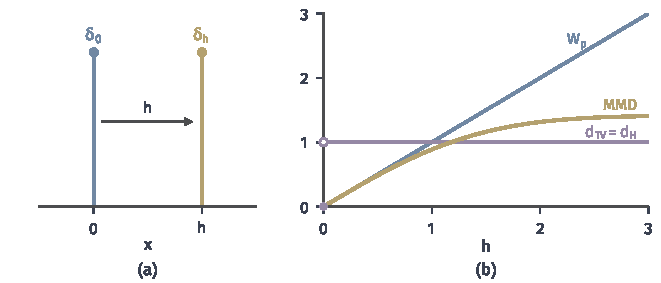
\includegraphics[width=112mm]{figures/07-probability/04-distribution-analysis/matplotlib/dcomp-point-shift/figure.pdf}
 \caption{单点分布的平移。(a)$\delta_0$与$\delta_h$。(b)作为$h$的函数：$W_p=h$（蓝，对所有$p$相同），$d_{\mathrm{TV}}=d_{\mathrm{H}}=1$（紫，$h=0$时为$0$），$\sigma=1$高斯核的$\operatorname{MMD}=\sqrt{2-2\mathrm{e}^{-h^{2}/2}}$（黄）。KL散度对每个$h>0$都是$+\infty$。}
 \label{fig:dcomp-point-shift}
\end{BookInlineFigure}

\paragraph{例表上的搬运}
把例表的三个取值看成实数轴上的位置$0,1,2$，距离取$\lvert x-y\rvert$。耦合是一个$3\times3$的非负矩阵$\bm{\pi}$，行和为$\bm{p}=(0.6,0.3,0.1)$，列和为$\bm{q}=(0.3,0.3,0.4)$，成本是$\sum_{i,j}\bm{\pi}_{i,j}\lvert i-j\rvert^{p}$（下标从$0$起）。图~\ref{fig:dcomp-coupling-plans}给出三个耦合。

\begin{BookInlineFigure}
 \centering
 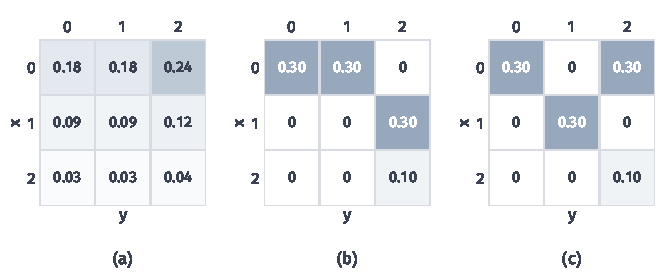
\includegraphics[width=112mm]{figures/07-probability/04-distribution-analysis/matplotlib/dcomp-coupling-plans/figure.pdf}
 \caption{例表的三个耦合，行是$x$（$P$），列是$y$（$Q$），颜色越深质量越大。(a)独立耦合$\bm{p}\bm{q}^{\top}$：$\sum\bm{\pi}_{i,j}\lvert i-j\rvert=0.96$，$\sum\bm{\pi}_{i,j}\lvert i-j\rvert^{2}=1.5$。(b)逐格搬运：两项成本都是$0.6$。(c)跳格搬运：一阶成本$0.6$，二阶成本$1.2$。}
 \label{fig:dcomp-coupling-plans}
\end{BookInlineFigure}

独立耦合让每一份质量都随机地去往目的地，许多质量被不必要地搬远，一阶成本是$0.96$。逐格搬运把点$0$多出的$0.3$搬到点$1$，再把点$1$原有的$0.3$搬到点$2$；跳格搬运直接把$0.3$从$0$搬到$2$，点$1$不动，见图~\ref{fig:dcomp-transport-arrows}。两种方案的一阶成本都是$0.6$。

\begin{BookInlineFigure}
 \centering
 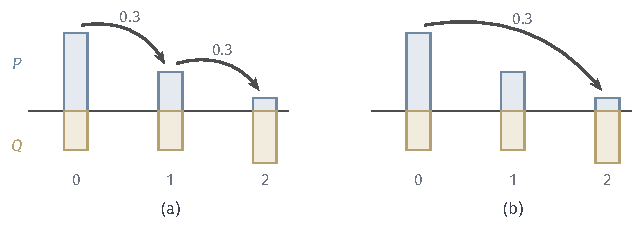
\includegraphics[width=108mm]{figures/07-probability/04-distribution-analysis/tikz/dcomp-transport-arrows/figure.pdf}
 \caption{例表的两种搬运方案，蓝柱向上是$P$，黄柱向下是$Q$，箭头上的数是搬运的质量。(a)逐格搬运：$0\to1$与$1\to2$各$0.3$。(b)跳格搬运：$0\to2$搬$0.3$。}
 \label{fig:dcomp-transport-arrows}
\end{BookInlineFigure}

$0.6$已经是最小值。对任何耦合$(X,Y)$，期望的绝对值不超过绝对值的期望，所以
\[
 \mathbb{E}\lvert X-Y\rvert\geq\lvert\mathbb{E}[X]-\mathbb{E}[Y]\rvert=\lvert0.5-1.1\rvert=0.6 ,
\]
所以$W_1(P,Q)=0.6$，两个方案都最优。二阶成本把两者分开了。记$a=\bm{\pi}_{0,1}$，$b=\bm{\pi}_{0,2}$，$c=\bm{\pi}_{1,2}$。点$0$只能留下$0.3$，所以至少$0.3$离开它，$a+b\geq0.3$；点$2$原有的$0.1$至多满足它的需要$0.4$中的$0.1$，所以$b+c\geq0.3$。成本矩阵中其余元素非负，于是
\[
 \sum_{i,j}\bm{\pi}_{i,j}\lvert i-j\rvert^{2}\geq a+4b+c=(a+b)+(b+c)+2b\geq0.6 ,
\]
等号要求$b=0$，$a=c=0.3$，正是逐格搬运。所以$W_2(P,Q)=\sqrt{0.6}\approx0.7746$。$p=1$时成本按距离线性计，一次跳两格与两次各跳一格花费相同；$p>1$时长距离被加倍惩罚，最优方案倾向于让每份质量只走短路。

这个例子也说明了定义中的“下确界”不能省略。如果$X,Y$已经由某个实验在同一概率空间上给出，它们的联合分布只是$\Pi(P,Q)$中的一个元素，$\mathbb{E}\lvert X-Y\rvert^{p}$通常大于$W_p^{p}$。Wasserstein距离只依赖两个边缘分布，与它们碰巧以怎样的方式一起出现无关。第~\ref{sec:dcomp-wasserstein-convergence}节会再回到这一点。

\paragraph{离散度量下的总变差}
在任意集合上取离散度量$d(x,y)=\mathbf{1}_{\{x\neq y\}}$，搬运成本只问“动没动”，不问距离。这时$W_1$正是总变差：
\begin{equation}
 \inf_{\pi\in\Pi(P,Q)}\pi\bigl(\{(x,y):x\neq y\}\bigr)=d_{\mathrm{TV}}(P,Q) .
 \label{eq:dcomp-maximal-coupling}
\end{equation}
一方面，对任何耦合$(X,Y)$与事件$A$，
\[
 P(A)-Q(A)=\mathbb{P}(X\in A)-\mathbb{P}(Y\in A)\leq\mathbb{P}(X\in A,\,Y\notin A)\leq\mathbb{P}(X\neq Y),
\]
所以左边不小于$d_{\mathrm{TV}}$。另一方面可以构造达到它的耦合。记$\delta=d_{\mathrm{TV}}(P,Q)$，设$0<\delta<1$（$\delta=0$时取$X=Y$，$\delta=1$时任何耦合都满足$\mathbb{P}(X\neq Y)\leq1$）。以概率$1-\delta$令$X=Y$，按密度$\min(p,q)/(1-\delta)$抽取；以概率$\delta$让$X$按密度$(p-q)^{+}/\delta$、$Y$按密度$(q-p)^{+}/\delta$独立抽取。由式~\eqref{eq:dcomp-tv-density}，这些都是概率密度。$X$的密度是$\min(p,q)+(p-q)^{+}=p$，$Y$的密度同理是$q$；第二种情形下$X$落在$\{p>q\}$而$Y$落在$\{q>p\}$，必然不等，所以$\mathbb{P}(X\neq Y)=\delta$。这样的耦合称为\term{最大耦合}（maximal coupling），它让两个变量以尽可能大的概率相等。总变差因此有了一个搬运解释：两个分布重叠的那部分质量原地不动，剩下的$d_{\mathrm{TV}}$那部分必须挪走。

\subsection{一阶距离的函数表示}
\label{sec:dcomp-kr}

例表上，$W_1$的下界来自函数$g(x)=x$的期望差。这不是巧合。若$g$是1-Lipschitz函数，即$\lvert g(x)-g(y)\rvert\leq d(x,y)$，则对任何耦合$(X,Y)$，
\[
 \mathbb{E}_{\mu}[g]-\mathbb{E}_{\nu}[g]=\mathbb{E}\bigl[g(X)-g(Y)\bigr]\leq\mathbb{E}\bigl[d(X,Y)\bigr] .
\]
对耦合取下确界，左边不超过$W_1(\mu,\nu)$。$g$的期望存在，因为$\lvert g(x)\rvert\leq\lvert g(x_0)\rvert+d(x,x_0)$，由一阶矩有限可积。所以每个1-Lipschitz函数都给出$W_1$的一个下界，而每个耦合都给出一个上界。两者在最优处相遇。

\begin{theorem}[Kantorovich--Rubinstein对偶]
\label{thm:dcomp-kantorovich-rubinstein}
设$(E,d)$是Polish空间，$\mu,\nu\in\mathcal{P}_1(E)$。则
\begin{equation}
 W_1(\mu,\nu)=\sup\Bigl\{\mathbb{E}_{\mu}[g]-\mathbb{E}_{\nu}[g]:\ \lvert g(x)-g(y)\rvert\leq d(x,y)\ \text{对一切}\ x,y\Bigr\} .
 \label{eq:dcomp-kr}
\end{equation}
\end{theorem}

上面已经证明了“$\geq$”。下面对两个分布都只有有限个支撑点的情形证明等号，一般情形的证明需要用有限支撑分布逼近并控制紧性，读者可查阅~\scite{math-villani2009transport}。这一结论称为\term{Kantorovich--Rubinstein对偶}（Kantorovich--Rubinstein duality）。

\begin{proof}[有限支撑情形的证明]
设$\mu=\sum_{i=1}^{m}a_i\delta_{x_i}$，$\nu=\sum_{j=1}^{n}b_j\delta_{y_j}$，记$c_{i,j}=d(x_i,y_j)$。两个边缘分别集中在$\{x_i\}$与$\{y_j\}$上，所以耦合集中在这些点对上，由矩阵$\bm{\pi}_{i,j}$描述。$W_1$是线性规划
\[
 \min_{\bm{\pi}\geq\bm{0}}\ \sum_{i,j}c_{i,j}\bm{\pi}_{i,j}\quad\text{s.t.}\quad\sum_{j}\bm{\pi}_{i,j}=a_i,\quad\sum_{i}\bm{\pi}_{i,j}=b_j
\]
的最优值。它的对偶问题是在约束$u_i+v_j\leq c_{i,j}$下最大化$\sum_ia_iu_i+\sum_jb_jv_j$。原问题可行（独立耦合）且目标有下界$0$，由线性规划的强对偶定理，对偶问题有最优解$(\bm{u},\bm{v})$，最优值等于$W_1$，可参考\BookChapterRef{chap:linear-programming}{卷五第2章“线性规划”}。

用对偶解构造一个函数：
\[
 g(z)=\min_{1\leq j\leq n}\bigl(d(z,y_j)-v_j\bigr),\qquad z\in E .
\]
每个$z\mapsto d(z,y_j)-v_j$都是1-Lipschitz函数，有限个1-Lipschitz函数的最小值仍是1-Lipschitz函数。由对偶约束，$u_i\leq c_{i,j}-v_j$对每个$j$成立，所以$g(x_i)\geq u_i$；取$z=y_j$并只看第$j$项，得$g(y_j)\leq-v_j$。于是
\[
 \mathbb{E}_{\mu}[g]-\mathbb{E}_{\nu}[g]=\sum_ia_ig(x_i)-\sum_jb_jg(y_j)\geq\sum_ia_iu_i+\sum_jb_jv_j=W_1(\mu,\nu) .
\]
与已经证明的“$\leq$”合起来，$g$达到了式~\eqref{eq:dcomp-kr}的上确界。
\end{proof}

证明中的$g$由一族“锥形”函数取下包络得到，每个锥以某个$y_j$为顶点、坡度为$1$、整体下移$v_j$。在例表上，$\mu=P$，$\nu=Q$，一个对偶最优解是$\bm{u}=(0,-1,-2)$，$\bm{v}=(0,1,2)$：约束$u_i+v_j=j-i\leq\lvert i-j\rvert$成立，目标值$-0.5+1.1=0.6$。构造出的$g$在$[0,2]$上就是$g(z)=-z$，见图~\ref{fig:dcomp-kr-dual}(b)；它与例表上的下界只差一个符号，$\mathbb{E}_{P}[g]-\mathbb{E}_{Q}[g]=0.6$。图中(a)画出两个分布函数，它们之间的面积也是$0.6$。实数轴上$W_1$与这块面积之间的一般关系属于一维运输问题，在第~\ref{chap:optimal-transport}章讨论。

\begin{BookInlineFigure}
 \centering
 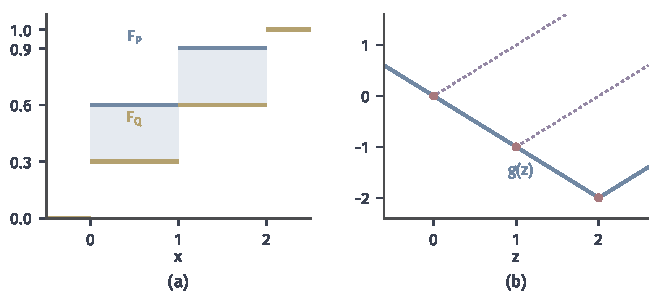
\includegraphics[width=112mm]{figures/07-probability/04-distribution-analysis/matplotlib/dcomp-kr-dual/figure.pdf}
 \caption{例表上的Kantorovich--Rubinstein对偶。(a)分布函数$F_P$（蓝）与$F_Q$（黄），两者之间浅蓝区域的面积为$0.6$。(b)紫色点线是三个锥$\lvert z-y_j\rvert-v_j$，$\bm{v}=(0,1,2)$；蓝线是它们的下包络$g$，红点是$g(x_i)=u_i$。}
 \label{fig:dcomp-kr-dual}
\end{BookInlineFigure}

式~\eqref{eq:dcomp-kr}把$W_1$放进了第~\ref{sec:dcomp-ipm}节的框架：它是由1-Lipschitz函数类生成的积分概率度量。与总变差的式~\eqref{eq:dcomp-tv-dual}对照，总变差的测试函数要求有界、允许跳跃；$W_1$的测试函数要求不能变化太快，但允许无界增长。前者对微小平移敏感，后者对远处的小质量敏感。

\paragraph{高阶距离不是积分概率度量}
$p>1$时，不能把式~\eqref{eq:dcomp-kr}中的$W_1$换成$W_p$，而且任何函数类都不行。原因是积分概率度量沿混合是线性的：对混合分布$\nu_\varepsilon=(1-\varepsilon)\mu+\varepsilon\nu$，每个$g$满足
\[
 \mathbb{E}_{\nu_\varepsilon}[g]-\mathbb{E}_{\mu}[g]=\varepsilon\bigl(\mathbb{E}_{\nu}[g]-\mathbb{E}_{\mu}[g]\bigr),
\]
取上确界得
\[
 d_{\mathcal{G}}(\mu,\nu_\varepsilon)=\varepsilon\,d_{\mathcal{G}}(\mu,\nu) .
\]
取$\mu=\delta_0$与$\nu=\delta_1$，混合分布把$\varepsilon$的质量放在$1$处。最优耦合让$1-\varepsilon$的质量留在原地，把$\varepsilon$的质量搬动距离$1$，所以
\[
 W_p(\mu,\nu_\varepsilon)=\varepsilon^{1/p} .
\]
$p=1$时它是$\varepsilon$，与线性相容；$p=2$时是$\sqrt\varepsilon$，见图~\ref{fig:dcomp-wp-mixture}。若$W_2=d_{\mathcal{G}}$对某个函数类成立，就会有$\sqrt\varepsilon=\varepsilon\cdot1$对一切$\varepsilon\in(0,1)$成立，矛盾。$W_p$对“少量质量走很远”的惩罚是非线性的，这是$p$次方成本带来的。

\begin{BookInlineFigure}
 \centering
 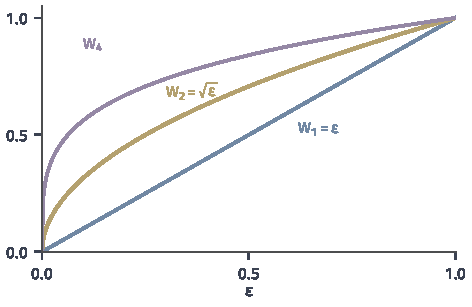
\includegraphics[width=80mm]{figures/07-probability/04-distribution-analysis/matplotlib/dcomp-wp-mixture/figure.pdf}
 \caption{$\delta_0$与$(1-\varepsilon)\delta_0+\varepsilon\delta_1$之间的$W_p=\varepsilon^{1/p}$：$p=1$（蓝），$p=2$（黄），$p=4$（紫）。任何积分概率度量沿这条混合线段都是$\varepsilon$的线性函数，只有$p=1$相容。}
 \label{fig:dcomp-wp-mixture}
\end{BookInlineFigure}

\section{期望误差}
\label{sec:dcomp-expectation}

比较分布往往是为了一个具体目的：用$Q$代替$P$计算某个平均$\mathbb{E}_{P}[g]$，误差有多大？前面几节已经分别得到有界函数、Lipschitz函数与RKHS函数的期望差表示。把这些结果放在一起，问题就变成：给定的$g$属于哪一类，范数是多少，该用哪个比较量。无界的$g$不属于这些类中的某几个，需要另外控制尾部；KL散度不是积分概率度量，要借助指数矩才能控制期望。

\subsection{函数范围内的误差}
\label{sec:dcomp-function-bounds}

把式~\eqref{eq:dcomp-tv-osc}、式~\eqref{eq:dcomp-kr}与式~\eqref{eq:dcomp-mmd-def}中的函数类按范数缩放，就得到三个上界。

\begin{theorem}[三类函数的期望差]
\label{thm:dcomp-three-bounds}
设$P,Q$是同一空间上的概率分布。
\begin{enumerate}
 \item 若$g$可测且有界，则期望差的绝对值不超过$\operatorname{osc}(g)\,d_{\mathrm{TV}}(P,Q)$。
 \item 若空间是Polish空间，$P,Q\in\mathcal{P}_1$，$g$是Lipschitz函数，常数为$\operatorname{Lip}(g)$，则
 \begin{equation}
  \bigl\lvert\mathbb{E}_{P}[g]-\mathbb{E}_{Q}[g]\bigr\rvert\leq\operatorname{Lip}(g)\,W_1(P,Q) .
  \label{eq:dcomp-lip-bound}
 \end{equation}
 \item 若$k$满足定理~\ref{thm:dcomp-kernel-mean}的条件，$P,Q$满足式~\eqref{eq:dcomp-kernel-moment}，$g\in\mathcal{H}$，则
 \begin{equation}
  \bigl\lvert\mathbb{E}_{P}[g]-\mathbb{E}_{Q}[g]\bigr\rvert\leq\lVert g\rVert_{\mathcal{H}}\operatorname{MMD}_k(P,Q) .
  \label{eq:dcomp-rkhs-bound}
 \end{equation}
\end{enumerate}
\end{theorem}

\begin{proof}
第一条即式~\eqref{eq:dcomp-tv-osc}。第二条：$\operatorname{Lip}(g)=0$时$g$为常数，两边为零；否则$g/\operatorname{Lip}(g)$是1-Lipschitz函数，由式~\eqref{eq:dcomp-kr}得结论，$g$在$P,Q$下可积已在第~\ref{sec:dcomp-kr}节说明。第三条：$g=0$时两边为零；否则$g/\lVert g\rVert_{\mathcal{H}}$在单位球中，由式~\eqref{eq:dcomp-mmd-def}得结论。
\end{proof}

定理的三条要求不同的东西，选择哪一条取决于$g$的性质。示性函数$\mathbf{1}_{A}$有界，但有跳跃，不是Lipschitz函数，也不在高斯核的RKHS中（该空间中的函数都连续），只能用总变差。$g(x)=x$是1-Lipschitz函数，但无界；高斯核有界，由定理~\ref{thm:dcomp-kernel-mean}证明中的估计，$\lvert g(x)\rvert$不超过$\lVert g\rVert_{\mathcal{H}}\sqrt{k(x,x)}$，而高斯核的$k(x,x)=1$，所以它的RKHS只含有界函数，所以只能用$W_1$。光滑、有界的函数三条都可以用，这时要比较哪个上界更小。

\paragraph{同一个函数的三个上界}
取$P=\delta_0$，$Q=\delta_h$，$g(x)=\exp(-x^{2}/2)$，它是$\sigma=1$高斯核的截面$k(0,\cdot)$。由式~\eqref{eq:dcomp-reproducing}，$\lVert g\rVert_{\mathcal{H}}=\sqrt{k(0,0)}=1$；它的振幅为$1$；导数$-x\mathrm{e}^{-x^{2}/2}$的绝对值在$x=\pm1$处最大，Lipschitz常数是$\mathrm{e}^{-1/2}\approx0.6065$。真实的误差和三个上界分别是
\[
 1-\mathrm{e}^{-h^{2}/2},\qquad 1,\qquad\mathrm{e}^{-1/2}h,\qquad\sqrt{2-2\mathrm{e}^{-h^{2}/2}} .
\]
$h=0.5$时，真实误差约为$0.1175$，$W_1$上界约为$0.3033$，MMD上界约为$0.4848$，总变差上界是$1$。图~\ref{fig:dcomp-three-bounds}显示，小平移时$W_1$的界最紧，大平移时总变差的界最紧（误差本来就不会超过振幅），MMD的界在两者之间过渡。没有哪一个比较量对所有情形都最好。

\begin{BookInlineFigure}
 \centering
 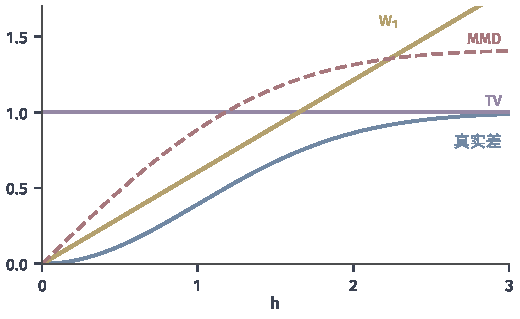
\includegraphics[width=88mm]{figures/07-probability/04-distribution-analysis/matplotlib/dcomp-three-bounds/figure.pdf}
 \caption{$P=\delta_0$，$Q=\delta_h$，$g(x)=\mathrm{e}^{-x^{2}/2}$时的期望误差。蓝线是真实误差$1-\mathrm{e}^{-h^{2}/2}$；紫线是总变差上界$\operatorname{osc}(g)\,d_{\mathrm{TV}}=1$，黄线是$W_1$上界$\mathrm{e}^{-1/2}h$，红色虚线是MMD上界$\sqrt{2-2\mathrm{e}^{-h^{2}/2}}$。}
 \label{fig:dcomp-three-bounds}
\end{BookInlineFigure}

\subsection{无界函数的尾部控制}
\label{sec:dcomp-tail}

许多需要计算的平均来自无界函数：均值、方差、多项式损失。分布在总变差或MMD意义下接近，只说明大部分质量摆放得差不多；极少的质量若落在很远的地方，无界函数会把它放大。下面先给出一个把问题拆开的不等式，再看反例。

\begin{lemma}[截断分解]
\label{lem:dcomp-truncation}
设$g$在$P,Q$下可积，$r>0$。记$g_r$为$g$在水平$r$处的截断，即把大于$r$的值改为$r$，小于$-r$的值改为$-r$。则
\begin{equation}
 \begin{aligned}
 \bigl\lvert\mathbb{E}_{P}[g]-\mathbb{E}_{Q}[g]\bigr\rvert&\leq\bigl\lvert\mathbb{E}_{P}[g_r]-\mathbb{E}_{Q}[g_r]\bigr\rvert\\
 &\quad+\mathbb{E}_{P}\bigl[\lvert g\rvert\mathbf{1}_{\{\lvert g\rvert>r\}}\bigr]+\mathbb{E}_{Q}\bigl[\lvert g\rvert\mathbf{1}_{\{\lvert g\rvert>r\}}\bigr] .
 \end{aligned}
 \label{eq:dcomp-truncation}
\end{equation}
\end{lemma}

\begin{proof}
$g-g_r$只在$\{\lvert g\rvert>r\}$上非零，那里$g-g_r$的绝对值是$\lvert g\rvert-r$，不超过$\lvert g\rvert$，所以
\[
 \bigl\lvert\mathbb{E}_{P}[g-g_r]\bigr\rvert\leq\mathbb{E}_{P}\bigl[\lvert g\rvert\mathbf{1}_{\{\lvert g\rvert>r\}}\bigr],
\]
对$Q$同理。把$g=g_r+(g-g_r)$代入期望差，用三角不等式即得。
\end{proof}

右边第一项是有界函数的期望差，可用前面的比较量控制，例如不超过$2r\,d_{\mathrm{TV}}(P,Q)$；若$g$是Lipschitz函数，$g_r$也是，并且常数不变，可以用$W_1$。后两项是两个分布各自的尾部，比较量对它们无能为力，必须由矩条件单独控制。对一列分布，需要的就是尾部的一致小。

\begin{theorem}[一致可积时期望收敛]
\label{thm:dcomp-ui-convergence}
设$d_{\mathrm{TV}}(P_n,P)\to0$，$g$在每个$P_n$与$P$下可积，并且
\begin{equation}
 \lim_{r\to\infty}\sup_{n}\mathbb{E}_{P_n}\bigl[\lvert g\rvert\mathbf{1}_{\{\lvert g\rvert>r\}}\bigr]=0 .
 \label{eq:dcomp-ui}
\end{equation}
则$\mathbb{E}_{P_n}[g]\to\mathbb{E}_{P}[g]$。
\end{theorem}

\begin{proof}
任给$\varepsilon>0$。由式~\eqref{eq:dcomp-ui}与$\mathbb{E}_{P}\lvert g\rvert<\infty$，可以取$r$，使式~\eqref{eq:dcomp-truncation}的两个尾部项对每个$P_n$与$P$都小于$\varepsilon$。由式~\eqref{eq:dcomp-truncation}与$\operatorname{osc}(g_r)\leq2r$，
\[
 \bigl\lvert\mathbb{E}_{P_n}[g]-\mathbb{E}_{P}[g]\bigr\rvert\leq2r\,d_{\mathrm{TV}}(P_n,P)+2\varepsilon .
\]
固定$r$令$n\to\infty$，上极限不超过$2\varepsilon$；$\varepsilon$任意，结论成立。
\end{proof}

条件~\eqref{eq:dcomp-ui}正是第~\ref{chap:random-variable-convergence}章的一致可积。多项式增长的函数可以用高一点的矩保证它。设$\lvert g(x)\rvert\leq C(1+\lvert x\rvert^{k})$，并且对某个$\delta>0$，各$P_n$的$k+\delta$阶绝对矩一致地不超过$M$。记$q=1+\delta/k$。在$\{\lvert g\rvert>r\}$上，$\lvert g\rvert\leq\lvert g\rvert^{q}/r^{q-1}$，又由$(a+b)^{q}\leq2^{q-1}(a^{q}+b^{q})$，
\[
 \mathbb{E}_{P_n}\bigl[\lvert g\rvert\mathbf{1}_{\{\lvert g\rvert>r\}}\bigr]\leq\frac{\mathbb{E}_{P_n}\lvert g\rvert^{q}}{r^{q-1}}\leq\frac{C^{q}2^{q-1}(1+M)}{r^{\delta/k}},
\]
关于$n$一致地趋于零。只有$k$阶矩有界是不够的，下面的例子说明这一点。

\paragraph{远处的小质量}
令$P_n=(1-\tfrac1n)\delta_0+\tfrac1n\delta_n$，与$\delta_0$比较。总变差是$1/n$，高斯核MMD约为$\sqrt2/n$，都趋于零。每个$P_n$只有两个支撑点，各阶矩都有限。可是均值与二阶矩是
\[
 \mathbb{E}_{P_n}[X]=\frac1n\cdot n=1,\qquad\mathbb{E}_{P_n}[X^{2}]=\frac1n\cdot n^{2}=n,
\]
不收敛到$\delta_0$下的$0$。尾部条件~\eqref{eq:dcomp-ui}对$g(x)=x$不成立：$n>r$时$\mathbb{E}_{P_n}[X\mathbf{1}_{\{X>r\}}]=1$。逐个分布的矩有限，不能代替一致的尾部控制。

$W_1$能看见这一份远处的质量：把$1/n$的质量从$n$搬回$0$，成本是$1$，所以$W_1(P_n,\delta_0)=1$，与均值的差一致，这正是式~\eqref{eq:dcomp-lip-bound}对$g(x)=x$的含义。但$W_1$也有看不见的东西。令
\[
 R_n=(1-n^{-2})\delta_0+n^{-2}\delta_n .
\]
把$n^{-2}$的质量搬动距离$n$，一阶与二阶的搬运成本分别给出
\[
 W_1(R_n,\delta_0)=\frac1n\to0,\qquad W_2(R_n,\delta_0)=\bigl(n^{-2}\cdot n^{2}\bigr)^{1/2}=1 ,
\]
而$R_n$的二阶矩恒为$1$，不趋于零。图~\ref{fig:dcomp-far-mass}画出这两族分布。控制$k$阶增长的函数，要用$k$阶的比较量或额外的一致可积条件。

\begin{BookInlineFigure}
 \centering
 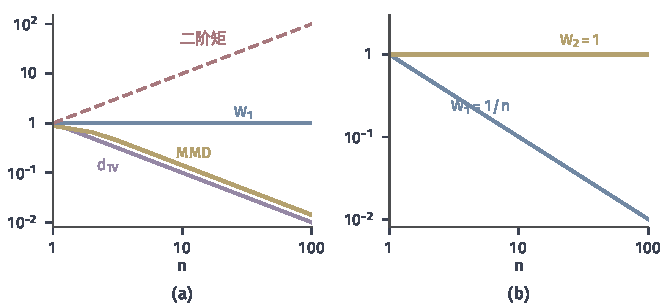
\includegraphics[width=112mm]{figures/07-probability/04-distribution-analysis/matplotlib/dcomp-far-mass/figure.pdf}
 \caption{远处的小质量，与$\delta_0$比较，双对数坐标。(a)$P_n=(1-\tfrac1n)\delta_0+\tfrac1n\delta_n$：$d_{\mathrm{TV}}=1/n$（紫），$\sigma=1$高斯核MMD（黄），$W_1=1$（蓝），二阶矩$n$（红色虚线）。(b)$R_n=(1-n^{-2})\delta_0+n^{-2}\delta_n$：$W_1=1/n$（蓝），$W_2=1$（黄）。}
 \label{fig:dcomp-far-mass}
\end{BookInlineFigure}

\subsection{KL与指数矩}
\label{sec:dcomp-kl-exp}

KL散度没有写成积分概率度量的形式，它能控制期望吗？先看有界函数：第~\ref{sec:dcomp-pinsker}节将证明KL散度控制总变差，于是它也控制有界函数的期望差。对无界函数，KL散度单独不够，还需要参考分布$Q$下的指数矩。关键工具是把$Q$按$\mathrm{e}^{g}$重新加权。

设$g$可测，$Z=\mathbb{E}_{Q}[\mathrm{e}^{g}]<\infty$。定义新的分布$Q_g$，
\begin{equation}
 \frac{\mathrm{d}Q_g}{\mathrm{d}Q}=\frac{\mathrm{e}^{g}}{Z} .
 \label{eq:dcomp-tilt}
\end{equation}
它把$Q$的质量向$g$大的地方倾斜，称为\term{指数倾斜}（exponential tilting）。密度$\mathrm{e}^{g}/Z$处处为正，所以$Q$与$Q_g$互相绝对连续。

\begin{lemma}[KL与对数矩母函数]
\label{lem:dcomp-dv}
设$D_{\mathrm{KL}}(P\Vert Q)<\infty$，$\mathbb{E}_{Q}[\mathrm{e}^{g}]<\infty$，$\mathbb{E}_{P}\lvert g\rvert<\infty$。则
\begin{equation}
 \mathbb{E}_{P}[g]\leq D_{\mathrm{KL}}(P\Vert Q)+\ln\mathbb{E}_{Q}\bigl[\mathrm{e}^{g}\bigr] .
 \label{eq:dcomp-dv}
\end{equation}
\end{lemma}

\begin{proof}
$P\ll Q$，$Q\ll Q_g$，所以$P\ll Q_g$，并且由密度的链式法则与式~\eqref{eq:dcomp-tilt}，
\[
 \ln\frac{\mathrm{d}P}{\mathrm{d}Q_g}=\ln\frac{\mathrm{d}P}{\mathrm{d}Q}-g+\ln Z .
\]
$D_{\mathrm{KL}}(P\Vert Q)$有限且对数比的负部可积，所以$\ln(\mathrm{d}P/\mathrm{d}Q)$在$P$下可积；$g$也可积。对上式在$P$下逐项取期望，并用Gibbs不等式，
\[
 0\leq D_{\mathrm{KL}}(P\Vert Q_g)=D_{\mathrm{KL}}(P\Vert Q)-\mathbb{E}_{P}[g]+\ln Z .
\]
移项即得。
\end{proof}

不等式~\eqref{eq:dcomp-dv}只是把KL的非负性用在倾斜后的参考分布上。它的含义是：$P$相对$Q$偏离不大时，$g$在$P$下的平均不会远超“$Q$下的指数平均”。为了得到期望差，对$g$减去它在$Q$下的均值并乘以参数$\lambda$。

\begin{theorem}[KL控制的期望差]
\label{thm:dcomp-kl-expectation}
设$D_{\mathrm{KL}}(P\Vert Q)<\infty$，$g$在$P,Q$下可积，记
\begin{equation}
 \Lambda(\lambda)=\ln\mathbb{E}_{Q}\Bigl[\exp\bigl(\lambda(g-\mathbb{E}_{Q}[g])\bigr)\Bigr] .
 \label{eq:dcomp-centered-cgf}
\end{equation}
则对每个使$\Lambda(\lambda)$有限的$\lambda>0$，
\begin{equation}
 \begin{gathered}
 \mathbb{E}_{P}[g]-\mathbb{E}_{Q}[g]\leq\frac{D_{\mathrm{KL}}(P\Vert Q)+\Lambda(\lambda)}{\lambda},\\
 \mathbb{E}_{Q}[g]-\mathbb{E}_{P}[g]\leq\frac{D_{\mathrm{KL}}(P\Vert Q)+\Lambda(-\lambda)}{\lambda} .
 \end{gathered}
 \label{eq:dcomp-kl-two-sides}
\end{equation}
特别地，若对一切实数$\lambda$有$\Lambda(\lambda)\leq\lambda^{2}s^{2}/2$，则
\begin{equation}
 \bigl\lvert\mathbb{E}_{P}[g]-\mathbb{E}_{Q}[g]\bigr\rvert\leq\sqrt{2s^{2}D_{\mathrm{KL}}(P\Vert Q)} .
 \label{eq:dcomp-kl-subgaussian}
\end{equation}
\end{theorem}

\begin{proof}
把引理~\ref{lem:dcomp-dv}用于$\lambda(g-\mathbb{E}_{Q}[g])$，它在$P$下可积，在$Q$下的指数矩是$\mathrm{e}^{\Lambda(\lambda)}$：
\[
 \lambda\bigl(\mathbb{E}_{P}[g]-\mathbb{E}_{Q}[g]\bigr)\leq D_{\mathrm{KL}}(P\Vert Q)+\Lambda(\lambda) .
\]
除以$\lambda>0$得第一式。把同样的推理用于$-g$，它的中心化对数矩母函数是$\Lambda(-\lambda)$，得第二式。在次高斯条件下，两式右端都不超过$D/\lambda+\lambda s^{2}/2$（记$D=D_{\mathrm{KL}}(P\Vert Q)$）。$D>0$时取$\lambda=\sqrt{2D}/s$使它最小，最小值为$\sqrt{2s^{2}D}$；$D=0$时$P=Q$，两边都是零。
\end{proof}

\paragraph{高斯平移}
取$Q=\mathcal{N}(0,1)$与$g(x)=x$。中心化对数矩母函数是$\Lambda(\lambda)=\lambda^{2}/2$，次高斯条件以$s=1$成立。倾斜后的$Q_g$在$g=\lambda x$时是$\mathcal{N}(\lambda,1)$：$\mathrm{e}^{\lambda x}$乘以标准高斯密度，配方后正是均值为$\lambda$的高斯密度。再取$P$为均值$m$、方差$1$的高斯分布，由式~\eqref{eq:dcomp-kl-gauss}，KL散度是$m^{2}/2$，式~\eqref{eq:dcomp-kl-subgaussian}给出
\[
 \lvert\mathbb{E}_{P}[X]-\mathbb{E}_{Q}[X]\rvert\leq\sqrt{2\cdot m^{2}/2}=\lvert m\rvert ,
\]
等号成立，上界不能改进。若$P=\mathcal{N}(m,s'^{2})$，均值差仍是$m$，而KL散度多了方差失配的部分，上界变松；$m=1$时，$s'=\tfrac12$与$s'=2$的上界分别约为$1.279$与$1.617$。图~\ref{fig:dcomp-kl-tilt}画出倾斜后的分布与这些上界。

\begin{BookInlineFigure}
 \centering
 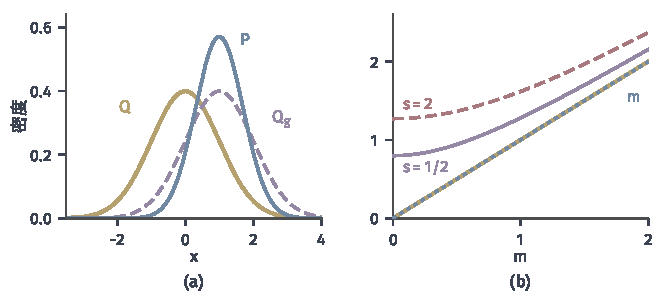
\includegraphics[width=112mm]{figures/07-probability/04-distribution-analysis/matplotlib/dcomp-kl-tilt/figure.pdf}
 \caption{KL散度与指数矩，$Q=\mathcal{N}(0,1)$，$g(x)=x$。(a)$Q$（黄），按$\mathrm{e}^{x}$倾斜后的$Q_g=\mathcal{N}(1,1)$（紫色虚线），以及$P=\mathcal{N}(1,0.7^{2})$（蓝）。(b)$P=\mathcal{N}(m,s'^{2})$时的真实均值差$m$（蓝色点线）与上界$\sqrt{2D_{\mathrm{KL}}(P\Vert Q)}$：$s'=1$（黄，与真实值重合），$s'=\tfrac12$（紫），$s'=2$（红色虚线）。}
 \label{fig:dcomp-kl-tilt}
\end{BookInlineFigure}

\paragraph{方向必须对应}
定理中的指数矩是在$Q$下计算的，而$Q$正是$D_{\mathrm{KL}}(P\Vert Q)$的第二个参数。只知道KL散度小、却不知道$Q$下的指数矩，期望可以相差无穷。在正整数上取
\[
 q_k=c\,k^{-3},\qquad r_k=\frac{6}{\pi^{2}}k^{-2},\qquad P_\varepsilon=(1-\varepsilon)Q+\varepsilon R ,
\]
其中$c\approx0.8319$。$Q$的均值是$c\sum_kk^{-2}\approx1.368$，有限，但它的尾部是多项式型的，$\mathbb{E}_{Q}[\mathrm{e}^{\lambda X}]$对任何$\lambda>0$都是无穷大。$R$的均值是$\tfrac{6}{\pi^{2}}\sum_kk^{-1}=+\infty$，所以$\mathbb{E}_{P_\varepsilon}[X]=+\infty$。另一方面，由$t\ln t$的凸性，
\[
 D_{\mathrm{KL}}(P_\varepsilon\Vert Q)=\mathbb{E}_{Q}\Bigl[f\Bigl((1-\varepsilon)+\varepsilon\frac{\mathrm{d}R}{\mathrm{d}Q}\Bigr)\Bigr]\leq(1-\varepsilon)f(1)+\varepsilon D_{\mathrm{KL}}(R\Vert Q),
\]
其中$f(t)=t\ln t$。而$D_{\mathrm{KL}}(R\Vert Q)=\sum_kr_k\ln(r_k/q_k)$中$\ln(r_k/q_k)$只按$\ln k$增长，级数收敛，数值约为$0.2563$。所以$P_\varepsilon$相对于$Q$的KL散度不超过$0.2563\,\varepsilon$，可以任意小，均值差却是无穷大。若指数矩只在$P$下有限，应当交换两个分布的角色，改用$D_{\mathrm{KL}}(Q\Vert P)$。

\section{比较量与收敛}
\label{sec:dcomp-convergence}

设$P_1,P_2,\dots$与$P$是一列分布，某个比较量$\rho(P_n,P)$趋于零。这能推出什么？能否推出另一个比较量也趋于零，能否推出第~\ref{chap:weak-convergence-of-distributions}章的弱收敛，矩是否也跟着收敛？本节逐一回答。弱收敛的定义与判别沿用那一章：$P_n\xrightarrow{\mathrm{w}}P$指对每个有界连续函数$f$，$\int f\,\mathrm{d}P_n\to\int f\,\mathrm{d}P$。那一章在$\mathbb{R}^{d}$上陈述；在一般度量空间上，定义只需把$\mathbb{R}^{d}$换成该空间，Portmanteau定理中“有界Lipschitz函数的期望收敛即可”这一判据的证明不变。

\subsection{散度与总变差的控制}
\label{sec:dcomp-pinsker}

先比较本身。总变差是最常用的标尺，KL散度和Hellinger距离与它有什么数量关系？本小节的对数一律取自然对数，总变差按定义~\ref{def:dcomp-tv}的约定，系数改变时下面的常数要相应改变。

\begin{theorem}[Pinsker不等式]
\label{thm:dcomp-pinsker}
对任意概率分布$P,Q$，
\begin{equation}
 d_{\mathrm{TV}}(P,Q)\leq\sqrt{\tfrac12D_{\mathrm{KL}}(P\Vert Q)} .
 \label{eq:dcomp-pinsker}
\end{equation}
\end{theorem}

\begin{proof}
\emph{化为两点分布。}若KL散度为$+\infty$，结论成立。设它有限，取$A^{*}=\{p>q\}$，用确定映射$x\mapsto\mathbf{1}_{A^{*}}(x)$把两个分布变成$\{0,1\}$上的两点分布$\operatorname{Bern}(a)$与$\operatorname{Bern}(b)$，其中$a=P(A^{*})$，$b=Q(A^{*})$。由定理~\ref{thm:dcomp-tv-density}，$d_{\mathrm{TV}}(P,Q)=a-b$；由定理~\ref{thm:dcomp-data-processing}，KL散度在映射后不增。所以只需证明两点分布的不等式
\[
 h(b)=a\ln\frac{a}{b}+(1-a)\ln\frac{1-a}{1-b}-2(a-b)^{2}\geq0,\qquad 0<b<1 .
\]

\emph{两点分布的情形。}固定$a\in[0,1]$，把$h$看成$b$的函数。$h(a)=0$。求导，
\[
 h'(b)=-\frac{a}{b}+\frac{1-a}{1-b}+4(a-b)=(b-a)\Bigl(\frac{1}{b(1-b)}-4\Bigr) .
\]
$b(1-b)\leq\tfrac14$，括号内非负，所以$h'(b)$与$b-a$同号：$h$在$b<a$时下降，在$b>a$时上升，最小值是$h(a)=0$。于是
\[
 D_{\mathrm{KL}}(P\Vert Q)\geq2(a-b)^{2}=2d_{\mathrm{TV}}^{2}(P,Q),
\]
开方即得。$b=0$或$1$而$a\neq b$时散度为$+\infty$，不需讨论。
\end{proof}

式~\eqref{eq:dcomp-pinsker}称为\term{Pinsker不等式}（Pinsker's inequality）。证明的思路值得留意：最坏事件$A^{*}$把一般分布压缩成一次是非判断，后处理不增加散度，于是一般情形归结为两点分布上的一元不等式。在例表上，$\sqrt{0.2773/2}\approx0.3723\geq0.3$。交换方向用$D_{\mathrm{KL}}(Q\Vert P)\approx0.3466$，得到$0.4163\geq0.3$，同样成立，因为总变差对称，任一方向的KL散度都控制它。图~\ref{fig:dcomp-pinsker}(a)在两点分布上比较两边：$P=\operatorname{Bern}(t)$，$Q=\operatorname{Bern}(\tfrac12)$，$t$接近$\tfrac12$时两条曲线几乎重合，常数$\tfrac12$不能再改进。

Pinsker不等式只有一个方向。总变差小不能推出KL散度小，甚至不能推出它有限。设$Q$在格点$0$处概率为零，例如$Q$是$\{1,2,\dots,10\}$上的均匀分布，令
\[
 P_\varepsilon=(1-\varepsilon)Q+\varepsilon\delta_0 .
\]
$P_\varepsilon$把$Q$的$\varepsilon$份质量挪到了点$0$，总变差是$\varepsilon$；但$P_\varepsilon(\{0\})=\varepsilon>0=Q(\{0\})$，$P_\varepsilon$不绝对连续于$Q$，$D_{\mathrm{KL}}(P_\varepsilon\Vert Q)=+\infty$。无论$\varepsilon$多小，总变差都看不出这个零概率格点上的冲突，KL散度则对它给出无穷大。

Hellinger距离与总变差之间是双向控制。

\begin{theorem}[Hellinger距离与总变差]
\label{thm:dcomp-hellinger-tv}
对任意概率分布$P,Q$，
\begin{equation}
 d_{\mathrm{H}}^{2}(P,Q)\leq d_{\mathrm{TV}}(P,Q)\leq d_{\mathrm{H}}(P,Q)\sqrt{2-d_{\mathrm{H}}^{2}(P,Q)} .
 \label{eq:dcomp-hellinger-tv}
\end{equation}
并且
\begin{equation}
 D_{\mathrm{KL}}(P\Vert Q)\geq2d_{\mathrm{H}}^{2}(P,Q) .
 \label{eq:dcomp-kl-hellinger}
\end{equation}
\end{theorem}

\begin{proof}
用共同支配测度写出密度。对每一点，
\[
 \lvert p-q\rvert=\lvert\sqrt{p}-\sqrt{q}\rvert\,(\sqrt{p}+\sqrt{q}),
\]
而右边第一个因子不超过第二个因子，所以$(\sqrt{p}-\sqrt{q})^{2}\leq\lvert p-q\rvert$。积分并乘以$\tfrac12$，得到左边的不等式。

对右边，用同一个分解与Cauchy--Schwarz不等式，
\[
 \frac12\int\lvert p-q\rvert\,\mathrm{d}\lambda\leq\frac12\Bigl(\int(\sqrt{p}-\sqrt{q})^{2}\,\mathrm{d}\lambda\Bigr)^{1/2}\Bigl(\int(\sqrt{p}+\sqrt{q})^{2}\,\mathrm{d}\lambda\Bigr)^{1/2} .
\]
第一个因子是$\sqrt2\,d_{\mathrm{H}}$；展开第二个因子中的平方，它是$(2+2B)^{1/2}$，由式~\eqref{eq:dcomp-hellinger-bc}，$B=1-d_{\mathrm{H}}^{2}$，所以第二个因子是$\sqrt2\,(2-d_{\mathrm{H}}^{2})^{1/2}$。代入即得右边的不等式。

最后，由定理~\ref{thm:dcomp-renyi-order}与式~\eqref{eq:dcomp-renyi-special}，$D_{\mathrm{KL}}\geq D_{1/2}=-2\ln B$，再由$-\ln B\geq1-B=d_{\mathrm{H}}^{2}$得式~\eqref{eq:dcomp-kl-hellinger}。
\end{proof}

在例表上，$d_{\mathrm{H}}^{2}\approx0.0757$，$d_{\mathrm{H}}\sqrt{2-d_{\mathrm{H}}^{2}}\approx0.3818$，总变差$0.3$确实夹在中间。式~\eqref{eq:dcomp-hellinger-tv}说明$d_{\mathrm{TV}}(P_n,P)\to0$当且仅当$d_{\mathrm{H}}(P_n,P)\to0$，两者定义的收敛相同，只是速度可能不同：一个是另一个的平方量级。图~\ref{fig:dcomp-pinsker}(b)在高斯平移族上画出这三条曲线以及Pinsker上界。

\begin{BookInlineFigure}
 \centering
 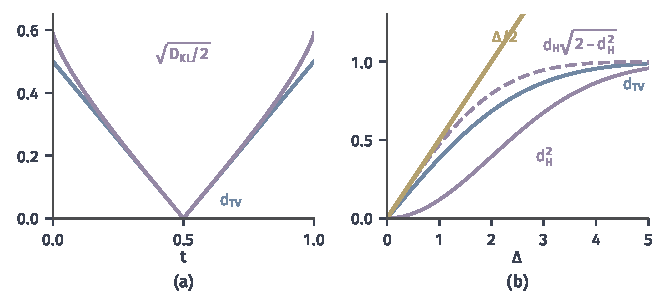
\includegraphics[width=112mm]{figures/07-probability/04-distribution-analysis/matplotlib/dcomp-pinsker/figure.pdf}
 \caption{散度对总变差的控制。(a)$P=\operatorname{Bern}(t)$，$Q=\operatorname{Bern}(\tfrac12)$：$d_{\mathrm{TV}}=\lvert t-\tfrac12\rvert$（蓝）与Pinsker上界$\sqrt{D_{\mathrm{KL}}(P\Vert Q)/2}$（紫）。(b)$P=\mathcal{N}(0,1)$，$Q=\mathcal{N}(\Delta,1)$：$d_{\mathrm{TV}}=2\Phi(\Delta/2)-1$（蓝），下界$d_{\mathrm{H}}^{2}=1-\mathrm{e}^{-\Delta^{2}/8}$（紫），上界$d_{\mathrm{H}}\sqrt{2-d_{\mathrm{H}}^{2}}$（紫色虚线），Pinsker上界$\Delta/2$（黄）。}
 \label{fig:dcomp-pinsker}
\end{BookInlineFigure}

\paragraph{总变差强于弱收敛}
若$d_{\mathrm{TV}}(P_n,P)\to0$，对每个有界连续$f$，由式~\eqref{eq:dcomp-tv-osc}，
\[
 \Bigl\lvert\int f\,\mathrm{d}P_n-\int f\,\mathrm{d}P\Bigr\rvert\leq2\lVert f\rVert_{\infty}\,d_{\mathrm{TV}}(P_n,P)\to0,
\]
所以$P_n\xrightarrow{\mathrm{w}}P$。反过来不成立。$\delta_{1/n}\xrightarrow{\mathrm{w}}\delta_0$，总变差却恒为$1$。一个更典型的例子是用离散分布逼近连续分布：令$U_n$是$n$个格点$(2k-1)/(2n)$（$k=1,\dots,n$）上的均匀分布，$U=\operatorname{Unif}(0,1)$。$U_n\xrightarrow{\mathrm{w}}U$，这是第~\ref{chap:weak-convergence-of-distributions}章Riemann和的例子（只把右端点换成中点）。但$U_n$集中在有限集上，那个集合的Lebesgue测度为零，两者相互奇异，$d_{\mathrm{TV}}(U_n,U)=1$，$D_{\mathrm{KL}}(U_n\Vert U)=+\infty$。

一阶Wasserstein距离却能正确地衡量这个逼近。把$(0,1)$分成$n$个长为$1/n$的小区间，每个格点恰在一个小区间的中点。把每个小区间里的均匀质量搬到它的中点，是一个耦合，平均搬运距离是
\[
 n\int_{0}^{1/n}\Bigl\lvert t-\frac{1}{2n}\Bigr\rvert\,\mathrm{d}t=\frac{1}{4n} .
\]
反过来，$g(x)=\min_k\lvert x-(2k-1)/(2n)\rvert$是到格点集合的距离，它是1-Lipschitz函数，在$U_n$下平均为$0$，在$U$下平均也是$1/(4n)$。由第~\ref{sec:dcomp-kr}节的上下界，$W_1(U_n,U)=1/(4n)$。图~\ref{fig:dcomp-lattice-metrics}比较三种量：总变差停在$1$，$W_1$按$1/n$下降，高斯核MMD下降得更快。

\begin{BookInlineFigure}
 \centering
 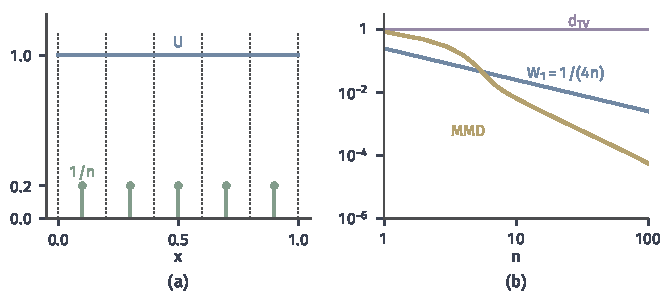
\includegraphics[width=112mm]{figures/07-probability/04-distribution-analysis/matplotlib/dcomp-lattice-metrics/figure.pdf}
 \caption{格点均匀分布逼近$\operatorname{Unif}(0,1)$。(a)$n=5$：绿色竖线是格点上的质量$1/n$，蓝线是$U$的密度，深灰点线是小区间的分界。(b)双对数坐标下的$d_{\mathrm{TV}}(U_n,U)=1$（紫），$W_1(U_n,U)=1/(4n)$（蓝），$\sigma=0.1$高斯核的$\operatorname{MMD}(U_n,U)$（黄，由式~\eqref{eq:dcomp-mmd-kernel}的三个核期望计算）。}
 \label{fig:dcomp-lattice-metrics}
\end{BookInlineFigure}

\subsection{Wasserstein收敛}
\label{sec:dcomp-wasserstein-convergence}

上一小节的格点例子中，$W_1\to0$与弱收敛同时成立。第~\ref{sec:dcomp-tail}节的$P_n=(1-\tfrac1n)\delta_0+\tfrac1n\delta_n$弱收敛到$\delta_0$（对有界连续$f$，$\int f\,\mathrm{d}P_n$与$f(0)$之差是$(f(n)-f(0))/n$，趋于零），$W_1(P_n,\delta_0)$却恒为$1$。差别在于一阶矩：$P_n$的均值恒为$1$，不收敛到$0$。下面的定理说明，这正是两者之间的全部差别。

\begin{theorem}[Wasserstein收敛的刻画]
\label{thm:dcomp-wasserstein-convergence}
设$(E,d)$是Polish空间，$1\leq p<\infty$，$\mu_n,\mu\in\mathcal{P}_p(E)$，$x_0\in E$。则$W_p(\mu_n,\mu)\to0$当且仅当
\begin{equation}
 \mu_n\xrightarrow{\mathrm{w}}\mu\quad\text{且}\quad\int d(x,x_0)^{p}\,\mu_n(\mathrm{d}x)\to\int d(x,x_0)^{p}\,\mu(\mathrm{d}x) .
 \label{eq:dcomp-wasserstein-convergence}
\end{equation}
\end{theorem}

下面证明“仅当”。“当”的方向需要从弱收敛与矩收敛出发构造代价趋于零的耦合，要用到$p$阶矩的一致可积与紧集上的逼近，篇幅较长，读者可查阅~\scite{math-villani2009transport}。

\begin{proof}[“仅当”的证明]
对每个$n$取耦合$\pi_n\in\Pi(\mu_n,\mu)$，使其成本不超过$W_p^{p}(\mu_n,\mu)+1/n$，并设随机变量对$(X_n,X)$服从$\pi_n$（每个$n$用各自的概率空间）。于是
\[
 \varepsilon_n=\bigl(\mathbb{E}\,d(X_n,X)^{p}\bigr)^{1/p}\to0 .
\]

\emph{弱收敛。}设$f$有界且Lipschitz，常数为$L$。由Lyapunov不等式$\mathbb{E}\,d(X_n,X)\leq\varepsilon_n$，
\[
 \Bigl\lvert\int f\,\mathrm{d}\mu_n-\int f\,\mathrm{d}\mu\Bigr\rvert\leq\mathbb{E}\bigl\lvert f(X_n)-f(X)\bigr\rvert\leq L\,\varepsilon_n\to0 .
\]
由Portmanteau定理的有界Lipschitz判据，$\mu_n\xrightarrow{\mathrm{w}}\mu$。

\emph{矩的收敛。}由三角不等式$d(X_n,x_0)\leq d(X_n,X)+d(X,x_0)$与$L^{p}$范数的Minkowski不等式，
\[
 \bigl(\mathbb{E}\,d(X_n,x_0)^{p}\bigr)^{1/p}\leq\varepsilon_n+\bigl(\mathbb{E}\,d(X,x_0)^{p}\bigr)^{1/p} .
\]
交换$X_n$与$X$的角色得到反向不等式，所以两个$p$阶矩的$p$次根之差不超过$\varepsilon_n$，趋于零。
\end{proof}

定理给出了一个清楚的分工：弱收敛管住质量在有界范围内的摆放，矩收敛管住远处有多少质量。第~\ref{sec:dcomp-tail}节的$R_n=(1-n^{-2})\delta_0+n^{-2}\delta_n$是一个检验：它弱收敛到$\delta_0$，一阶矩$1/n\to0$，二阶矩恒为$1$，所以$W_1\to0$而$W_2\not\to0$，与图~\ref{fig:dcomp-far-mass}(b)一致。阶数$p$越高，对远处质量的要求越严。

\paragraph{分布收敛不是取值收敛}
$W_p(\mu_n,\mu)\to0$说的是存在代价越来越小的耦合，而不是某个已经给定的联合实现中的误差变小。设$X\sim\mathcal{N}(0,1)$，$X'$是它的独立副本。$X'$与$X$同分布，$W_p(P_{X'},P_X)=0$，最优耦合是让两者相等。可是在已经给定的独立实现中，
\[
 \mathbb{E}\bigl[(X'-X)^{2}\bigr]=\operatorname{Var}(X')+\operatorname{Var}(X)=2 .
\]
把$X'$换成序列$X_n=X'$（每个$n$都相同），就有$W_2(P_{X_n},P_X)=0$对一切$n$成立，而$\mathbb{E}\lvert X_n-X\rvert^{2}=2$不趋于零。图~\ref{fig:dcomp-coupling-realization}用$300$个模拟点（种子$717$）对比这两种耦合，独立实现的样本平均平方差约为$1.94$。Wasserstein距离只是一个关于分布的结论，不能反推原有共同实现中的$L^{p}$误差；后者是第~\ref{chap:random-variable-convergence}章的$L^{p}$收敛，它要求$X_n$与$X$在同一概率空间上逐点接近。

\begin{BookInlineFigure}
 \centering
 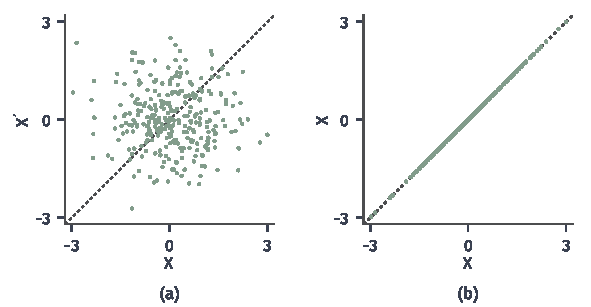
\includegraphics[width=100mm]{figures/07-probability/04-distribution-analysis/matplotlib/dcomp-coupling-realization/figure.pdf}
 \caption{$\mathcal{N}(0,1)$与自身的两种耦合，各$300$个模拟点（绿），种子$717$；深灰点线是$y=x$。(a)独立副本$(X,X')$，$\mathbb{E}(X-X')^{2}=2$，样本值约$1.94$。(b)恒等耦合$(X,X)$，成本为$0=W_2^{2}$。}
 \label{fig:dcomp-coupling-realization}
\end{BookInlineFigure}

\subsection{MMD收敛}
\label{sec:dcomp-mmd-convergence}

特征核保证$\operatorname{MMD}_k(P,Q)=0$当且仅当$P=Q$。一列分布的MMD趋于零是否等价于弱收敛，是另一回事：零点的辨识只涉及单个分布对，收敛还要求比较量不让质量悄悄跑到无穷远，也不对微小平移过度敏感。对$\mathbb{R}^{d}$上固定带宽的高斯核，两件事都成立。

\begin{theorem}[高斯核MMD刻画弱收敛]
\label{thm:dcomp-mmd-weak}
设$\sigma>0$，$k_\sigma$是$\mathbb{R}^{d}$上的高斯核，$P_n,P$是$\mathbb{R}^{d}$上的概率分布。则
\begin{equation}
 \operatorname{MMD}_{k_\sigma}(P_n,P)\to0\quad\Longleftrightarrow\quad P_n\xrightarrow{\mathrm{w}}P .
 \label{eq:dcomp-mmd-weak}
\end{equation}
\end{theorem}

\begin{proof}
\emph{弱收敛推出MMD趋于零。}取相互独立的$\bm{X}_n,\bm{X}_n'\sim P_n$与$\bm{X},\bm{X}'\sim P$。由第~\ref{chap:weak-convergence-of-distributions}章独立分量的联合极限，$(\bm{X}_n,\bm{X}_n')$与$(\bm{X}_n,\bm{X})$都依分布收敛到$(\bm{X},\bm{X}')$。$k_\sigma$在$\mathbb{R}^{d}\times\mathbb{R}^{d}$上有界连续，所以式~\eqref{eq:dcomp-mmd-kernel}中的三项分别趋于$\mathbb{E}[k_\sigma(\bm{X},\bm{X}')]$的$1$倍、$2$倍与$1$倍，和趋于零。

\emph{MMD趋于零推出胎紧。}记$\phi_n,\phi$为特征函数，$\lambda_\sigma$与$\gamma_\tau$分别为$\mathcal{N}(\bm{0},\sigma^{-2}\bm{I})$与$\mathcal{N}(\bm{0},\tau\bm{I})$的密度。令
\[
 h_\tau(\bm{x})=\exp\Bigl(-\frac{\tau}{2}\lVert\bm{x}\rVert_2^{2}\Bigr) .
\]
它是$\mathcal{N}(\bm{0},\tau\bm{I})$的特征函数，由Fubini定理，
\[
 \mathbb{E}_{P_n}[h_\tau]=\int\phi_n(\bm{\omega})\,\gamma_\tau(\bm{\omega})\,\mathrm{d}\bm{\omega} .
\]
于是，由Cauchy--Schwarz不等式与式~\eqref{eq:dcomp-mmd-spectral}，
\[
 \begin{aligned}
 \bigl\lvert\mathbb{E}_{P_n}[h_\tau]-\mathbb{E}_{P}[h_\tau]\bigr\rvert&\leq\int\lvert\phi_n-\phi\rvert\frac{\gamma_\tau}{\lambda_\sigma}\lambda_\sigma\,\mathrm{d}\bm{\omega}\\
 &\leq\operatorname{MMD}_{k_\sigma}(P_n,P)\Bigl(\int\frac{\gamma_\tau^{2}}{\lambda_\sigma}\,\mathrm{d}\bm{\omega}\Bigr)^{1/2} .
 \end{aligned}
\]
$\gamma_\tau^{2}/\lambda_\sigma$正比于$\exp(-(\tau^{-1}-\sigma^{2}/2)\lVert\bm{\omega}\rVert_2^{2})$，当$\tau<2/\sigma^{2}$时可积。所以对这样的$\tau$，$\mathbb{E}_{P_n}[h_\tau]\to\mathbb{E}_{P}[h_\tau]$。

任给$\varepsilon>0$。$\tau\downarrow0$时$h_\tau\uparrow1$，由单调收敛定理可取$\tau<2/\sigma^{2}$使$1-\mathbb{E}_{P}[h_\tau]<\varepsilon$，再取$N$使$n\geq N$时$1-\mathbb{E}_{P_n}[h_\tau]<2\varepsilon$。取$r$使$\mathrm{e}^{-\tau r^{2}/2}\leq\tfrac12$。在$\{\lVert\bm{x}\rVert_2>r\}$上$1-h_\tau\geq\tfrac12$，由Markov不等式，
\[
 P_n\bigl(\lVert\bm{X}\rVert_2>r\bigr)\leq2\bigl(1-\mathbb{E}_{P_n}[h_\tau]\bigr)<4\varepsilon,\qquad n\geq N .
\]
前$N-1$个分布各自胎紧，增大$r$即可一并照顾，所以$\{P_n\}$胎紧。

\emph{子列的极限只能是$P$。}设某个子列$P_{n_j}\xrightarrow{\mathrm{w}}R$。由连续性定理，$\phi_{n_j}\to\phi_R$逐点成立，并且都以$1$为界，由控制收敛定理，$\phi_{n_j}$在$L^{2}(\Lambda_\sigma)$中收敛到$\phi_R$。又由式~\eqref{eq:dcomp-mmd-spectral}，$\phi_{n_j}$在$L^{2}(\Lambda_\sigma)$中到$\phi$的距离就是MMD，趋于零。由$L^{2}(\Lambda_\sigma)$中的三角不等式，$\phi_R=\phi$在$\Lambda_\sigma$几乎处处成立。与定理~\ref{thm:dcomp-gauss-characteristic}的论证相同，$R=P$。由第~\ref{chap:weak-convergence-of-distributions}章的子列原则，$P_n\xrightarrow{\mathrm{w}}P$。
\end{proof}

证明里高斯核起了两个作用。谱权重$\Lambda_\sigma$处处为正，保证极限唯一；它的尾部比$\gamma_\tau^{2}$的尾部衰减得慢，使原点附近的特征函数，也就是“质量是否跑远”的信息，能被MMD控制住。

\paragraph{结论的边界}
高斯核MMD刻画的是弱收敛，不多也不少。它不附带矩的收敛：$P_n=(1-\tfrac1n)\delta_0+\tfrac1n\delta_n$弱收敛到$\delta_0$，所以MMD趋于零（图~\ref{fig:dcomp-far-mass}(a)），均值却恒为$1$。要控制无界函数，仍需第~\ref{sec:dcomp-tail}节的尾部条件。

这个刻画也不能推广到所有特征核。在高斯核上加一个不连续的部分：令$f=\mathbf{1}_{(0,\infty)}$，
\[
 k(x,y)=k_1(x,y)+f(x)f(y),\qquad x,y\in\mathbb{R} .
\]
两个正定核之和仍是正定核，它有界，可以验证相应的RKHS可分、特征映射可测。由式~\eqref{eq:dcomp-mmd-kernel}，
\[
 \operatorname{MMD}_k^{2}(P,Q)=\operatorname{MMD}_{k_1}^{2}(P,Q)+\bigl(P(X>0)-Q(X>0)\bigr)^{2}\geq\operatorname{MMD}_{k_1}^{2}(P,Q),
\]
所以$k$仍是特征核。可是$\delta_{1/n}\xrightarrow{\mathrm{w}}\delta_0$，而第二项恒为$(1-0)^{2}=1$，$\operatorname{MMD}_k(\delta_{1/n},\delta_0)\geq1$不趋于零。不连续的核截面像示性函数一样对微小平移敏感。所以“MMD收敛等价于弱收敛”须同时核对空间与核的条件，例如核的连续性与有界性，不能只凭特征性得出。

\section{本章小结}
\label{sec:dcomp-summary}

章首的问题是：两份概率表$P=(0.6,0.3,0.1)$与$Q=(0.3,0.3,0.4)$差多少。本章的回答是，先问差别会在哪里造成后果，再选比较量。表~\ref{tab:dcomp-summary-example}把例表上算出的各个量放在一起。

\begin{BookInlineTable}
 \centering
 \caption{例表上的各比较量（自然对数；MMD用$\sigma=1$的高斯核）。}
 \label{tab:dcomp-summary-example}
 \begin{tabular}{lll}
  \toprule
  比较量 & 数值 & 回答的问题\\
  \midrule
  $d_{\mathrm{TV}}$ & $0.3$ & 同一事件的概率最多差多少\\
  $D_{\mathrm{KL}}(P\Vert Q)$，$D_{\mathrm{KL}}(Q\Vert P)$ & $0.2773$，$0.3466$ & 平均对数比，方向不同\\
  $d_{\mathrm{H}}$，$B$ & $0.2752$，$0.9243$ & 平方根密度的弦长与重叠\\
  $D_{\mathrm{JS}}$ & $0.0737$ & 相对平均分布的KL，有界\\
  $D_{1/2}$，$D_{2}$ & $0.1575$，$0.4220$ & 不同幂次加权的对数比\\
  $\operatorname{MMD}_k$ & $0.3945$ & 核均值之差\\
  $W_1$，$W_2$ & $0.6$，$0.7746$ & 搬运质量的最小成本\\
  \bottomrule
 \end{tabular}
\end{BookInlineTable}

四个角度各有所长。总变差控制所有事件与有界函数，不需要底层距离，但对微小平移与相互奇异的分布一律给出最大值。密度比较量在同一支配测度下比较同一位置的权重：KL散度有似然比的含义并且不对称，Hellinger距离是平方根密度之间的真正距离，JS散度借助平均分布保持有限，Rényi散度用阶数调节对大比值的敏感程度；它们中的$f$散度都满足后处理不增的性质。积分概率度量由测试函数类决定能看见什么，核均值把RKHS单位球上的上确界变成两个核均值之差的范数。Wasserstein距离保留底层几何，一阶时又是Lipschitz函数上的积分概率度量。

用于控制期望时，要先判断评价函数$g$的类型：有界函数配总变差，Lipschitz函数配$W_1$，RKHS中的函数配MMD；无界函数必须把尾部单独拿出来，用一致可积或高阶矩控制；用KL散度控制期望时，需要参考分布下的指数矩，并且方向要与散度的参数对应。

用于收敛时，各比较量之间的关系汇总在图~\ref{fig:dcomp-implication-map}中。KL散度通过Pinsker不等式控制总变差，总变差与Hellinger距离相互控制，总变差收敛推出弱收敛而反之不然；$W_p$收敛等于弱收敛加$p$阶矩收敛；$\mathbb{R}^{d}$上固定带宽的高斯核MMD收敛恰好等于弱收敛。反过来的每一个缺口都有反例：零概率格点使小总变差对应无穷KL，单点平移与格点逼近使弱收敛不带来总变差收敛，远处的小质量使弱收敛与MMD收敛不带来矩的收敛，不连续的特征核使MMD不再刻画弱收敛。

\begin{BookInlineFigure}
 \centering
 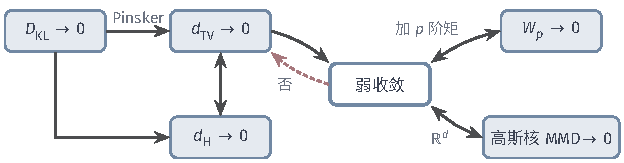
\includegraphics[width=106mm]{figures/07-probability/04-distribution-analysis/tikz/dcomp-implication-map/figure.pdf}
 \caption{本章证明或引用的收敛关系，均指$P_n$与固定的$P$之间的比较量趋于零。实线箭头表示蕴含，双向箭头表示等价（$W_p$需加上$p$阶矩收敛，高斯核MMD限于$\mathbb{R}^{d}$），红色虚线表示反向不成立。}
 \label{fig:dcomp-implication-map}
\end{BookInlineFigure}

第~\ref{chap:distribution-approximation}章在限定的候选族中寻找与目标最接近的分布时，就要用这里的比较量衡量误差，并按任务选择方向。第~\ref{chap:dependence-measures}章把联合分布与边缘乘积作比较，用KL散度得到互信息，用MMD得到HSIC。从有限样本估计这些比较量、评价估计误差并据此检验两个分布是否相同，属于卷八的内容。


\chapter{信息量}
\label{chap:information-measures}

一个结果按概率$\tfrac12,\tfrac14,\tfrac18,\tfrac18$出现在四个字母$a,b,c,d$中。朋友知道结果，我们只能问是非题。先问“是$a$吗”，有一半机会一题就猜中；否则再问“是$b$吗”，依此类推，平均要问$1.75$题。若四个字母等可能，平均就要问$2$题。分布越集中，平均要问的题越少。能不能用一个只依赖概率表的数，衡量一个随机结果平均含有多少不确定性？

再看两个相关的结果。一枚公平硬币$X$经过一条会以概率$\tfrac14$出错的线路，收到的是$Y$。看到$Y$以后，$X$并没有被完全确定，但比看到之前清楚了一些。清楚了多少？如果再把$Y$经过同样的线路传一次，或者把$Y$压缩成更粗的摘要，能不能反而更清楚？如果要从$Y$猜出$X$，错误概率最低能低到哪里？

本章研究这些问题。第一节从单个结果的意外程度出发，定义自信息与熵，先在离散情形建立它的基本性质，再说明对密度计算的微分熵改变了什么。第二、三节研究两个变量：联合熵与条件熵度量整体和剩余的不确定性，互信息度量观测带来的不确定性的减少，并用联合分布与边缘乘积的KL散度给出不依赖熵是否有限的一般定义。第四节讨论按一个参考分布分配对数代价时多付的部分，即交叉熵。

后四节用这些量研究信息处理的限制。数据处理不等式说明对观测作任何只依赖观测本身的处理都不能增加信息；Fano不等式把剩余的不确定性转成辨别错误的下界；在互信息难以直接计算时，用辨认真配对的辅助问题可以得到它的一个可计算的下界；最后讨论信息量随分布连续变化需要什么条件。

全章以自然对数为准，信息量的单位是nat；需要以“题数”或二进制位数解释时换成以$2$为底的对数，单位是bit。两个贯穿的小例子是上面的四字母表和公平硬币经过出错线路的二元表，后面还会用到一张不对称的$2\times2$联合表。怎样用最少的码字实际描述结果、怎样在有噪声的线路上可靠地传输，分别在第~\ref{chap:lossless-coding}章和第~\ref{chap:discrete-channel-capacity}章研究；本章只建立这些任务所用的量及其界。

\section{熵}
\label{sec:info-entropy}

天气预报说明天有雨，在雨季几乎不值得一提，在旱季却是大新闻。同一句话带来的信息多少，取决于它事先有多意外。本节先给单个结果的意外程度一个数值，再对所有可能结果取平均，得到衡量随机结果不确定性的熵。离散结果可以直接这样做；对有密度的连续结果照搬公式时，会多出一个依赖坐标尺度的量，需要单独说明。

\subsection{自信息}
\label{sec:info-self-information}

设某个结果发生的概率是$p\in(0,1]$。我们想给它指定一个数$c(p)$，表示“得知这个结果发生”所获得的信息量。至少有两个要求是自然的。

第一，越罕见的结果越意外，信息越多，所以$c$是$(0,1]$上的递减函数；必然发生的结果不带来信息，$c(1)=0$。第二，两个独立结果同时发生的概率是$pq$，分别得知它们和一起得知它们，获得的信息应当一样多，所以
\[
  c(pq)=c(p)+c(q),\qquad 0<p,q\leq1.
\]
回到章首的四字母表：结果$c$的概率是$\tfrac18$，它相当于连续三次“二选一”都选中某一边，每次概率$\tfrac12$；按第二个要求，它的信息量应是$\tfrac12$对应信息量的三倍。

\begin{theorem}[自信息的形式]
\label{thm:info-self-information-form}
设$c:(0,1]\to[0,\infty)$递减且对一切$p,q\in(0,1]$满足$c(pq)=c(p)+c(q)$，则存在常数$a\geq0$，使
\begin{equation}
  c(p)=-a\ln p,\qquad 0<p\leq1.
  \label{eq:info-self-information-form}
\end{equation}
\end{theorem}

\begin{proof}
令$b(u)=c(\mathrm{e}^{-u})$，$u\geq0$。指数函数把加法变成乘法，所以$c$的乘法关系变成$b$的加法关系：
\[
  b(u+v)=b(u)+b(v),\qquad u,v\geq0.
\]
$u$增大时$\mathrm{e}^{-u}$减小，$c$递减，所以$b$在$[0,\infty)$上递增。

先看有理点。由可加性，$b(0)=b(0)+b(0)$，故$b(0)=0$；对正整数$n$，$b(nu)=nb(u)$。取$u=1/m$，得$b(1)=m\,b(1/m)$，于是对正整数$n,m$，
\[
  b\Bigl(\frac{n}{m}\Bigr)=n\,b\Bigl(\frac1m\Bigr)=\frac{n}{m}\,b(1).
\]
记$a=b(1)\geq b(0)=0$，则$b(r)=ar$对一切非负有理数$r$成立。

再看一般的$u\geq0$。对任意有理数$r\leq u\leq s$，单调性给出$ar=b(r)\leq b(u)\leq b(s)=as$。让$r,s$从两侧趋于$u$，得$b(u)=au$。代回$u=-\ln p$，即得式~\eqref{eq:info-self-information-form}。
\end{proof}

证明里两个要求各起一个作用：可加性把$c$在有理点上的值全部确定下来，单调性把有理点之间的空隙填满。只有可加性而没有任何正则性时，满足$b(u+v)=b(u)+b(v)$的函数可以极不规则，结论就不再成立。常数$a$不受这两个要求约束，它只决定信息量的单位。

\begin{definition}[自信息]
\label{def:info-self-information}
设离散随机变量$X$的概率质量为$p_X$。对$p_X(x)>0$的取值$x$，称
\begin{equation}
  \iota(x)=-\ln p_X(x)
  \label{eq:info-self-information}
\end{equation}
为结果$x$的\term{自信息}（self-information），单位为\term{奈特}（nat）。若改用$-\log_2 p_X(x)$，单位为\term{比特}（bit）。
\end{definition}

两种单位只差一个正的常数倍：$-\log_2 p=-\ln p/\ln2$，所以
\[
  1\ \mathrm{bit}=\ln2\ \mathrm{nat}\approx0.693\ \mathrm{nat}.
\]
换单位不改变任何两个信息量的大小顺序，也不改变“相等”“为零”这类结论。本章用nat计算，以bit解释“是非题个数”。

比特的说法来自是非题。一个概率为$2^{-k}$的结果，自信息是$k$ bit，恰好相当于连续回答$k$个各占一半的是非题。图~\ref{fig:info-self-information}画出$-\ln p$，右侧刻度换成bit。$p$从$1$减小到$\tfrac12$只带来$1$ bit，而每再减半一次就多$1$ bit；概率趋于零时自信息趋于无穷。

\begin{BookInlineFigure}
  \centering
  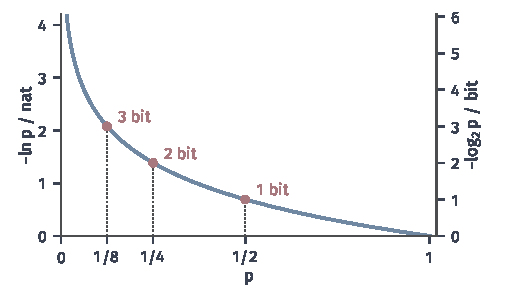
\includegraphics[width=86mm]{figures/07-probability/04-distribution-analysis/matplotlib/info-self-information/figure.pdf}
  \caption{自信息随概率的变化。蓝线为$-\ln p$，左轴以nat计，右轴为同一曲线以bit计的刻度。红点是四字母表中概率$\tfrac12,\tfrac14,\tfrac18$的结果，分别对应$1,2,3$ bit。}
  \label{fig:info-self-information}
\end{BookInlineFigure}

自信息是一次结果的属性。看到罕见结果时获得很多信息，但罕见结果很少出现；要衡量一个随机结果“平均”含有多少信息，还要按概率取平均。

\subsection{离散熵}
\label{sec:info-discrete-entropy}

章首的四字母表可以按图~\ref{fig:info-question-tree}的方式提问。每个结果所需的题数恰好是它以bit计的自信息：$a$一题，$b$两题，$c,d$各三题。平均题数是
\[
  \tfrac12\cdot1+\tfrac14\cdot2+\tfrac18\cdot3+\tfrac18\cdot3=1.75.
\]
这就是自信息的平均。对一般的概率表，题数必须是整数，不一定能与自信息一一相等；第~\ref{chap:lossless-coding}章证明，最好的提问方案平均题数与以bit计的熵相差不到一题。

\begin{BookInlineFigure}
  \centering
  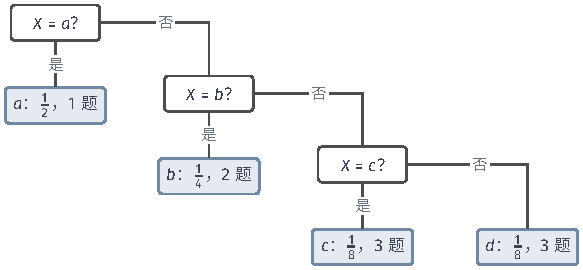
\includegraphics[width=98.7mm]{figures/07-probability/04-distribution-analysis/tikz/info-question-tree/figure.pdf}
  \caption{四字母表$(\tfrac12,\tfrac14,\tfrac18,\tfrac18)$的一种是非题提问方案。蓝框是确定下来的结果，框内为其概率与所需题数；每个结果的题数等于$-\log_2 p$，平均题数为$1.75$。}
  \label{fig:info-question-tree}
\end{BookInlineFigure}

\begin{definition}[离散熵]
\label{def:info-discrete-entropy}
设离散随机变量$X$取值于有限或可数集合$\mathcal{X}$，概率质量为$p_X$。$X$的\term{熵}（entropy）定义为
\begin{equation}
  H(X)=-\sum_{x\in\mathcal{X}}p_X(x)\ln p_X(x)=\mathbb{E}[-\ln p_X(X)],
  \label{eq:info-entropy}
\end{equation}
其中约定$0\ln0=0$。各项非负，和可以为$+\infty$。
\end{definition}

约定$0\ln0=0$有两个理由。概率为零的结果从不出现，不应影响平均；并且$t\ln t\to0$（$t\downarrow0$），约定与极限一致，加入或删去零概率的取值都不改变熵。熵只依赖概率值的集合，与取值叫什么无关：把$a,b,c,d$换成$1,2,3,4$或任意排列，熵不变。这一点与期望、方差不同，后者依赖取值本身。

四字母表的熵为
\[
  H(X)=\tfrac12\ln2+\tfrac14\ln4+2\cdot\tfrac18\ln8=\tfrac74\ln2\approx1.213\ \mathrm{nat},
\]
即$1.75$ bit。若四个字母等可能，熵为$\ln4\approx1.386$ nat，即$2$ bit。

\paragraph{有限字母表上的基本性质}
下面的性质说明熵确实符合“不确定性”的直觉：确定的结果没有不确定性，均匀分布最不确定，把两个分布混合起来不会更确定。

\begin{theorem}[有限字母表上熵的范围]
\label{thm:info-entropy-range}
设$X$取值于$m$个元素的集合$\mathcal{X}$。则
\begin{equation}
  0\leq H(X)\leq\ln m.
  \label{eq:info-entropy-range}
\end{equation}
左边等号当且仅当$X$以概率$1$取某一个值；右边等号当且仅当$X$在$\mathcal{X}$上均匀分布。
\end{theorem}

\begin{proof}
每个$p_X(x)\in[0,1]$，所以$-p_X(x)\ln p_X(x)\geq0$，和非负。各项为零当且仅当$p_X(x)\in\{0,1\}$，而概率之和为$1$，这只能是某一个$x$的概率为$1$。

右边用不等式$\ln t\leq t-1$（$t>0$），它在$t=1$处取等号，其余处严格成立。记$S=\{x:p_X(x)>0\}$。对$x\in S$取$t=1/(m\,p_X(x))$，得到
\[
  H(X)-\ln m=\sum_{x\in S}p_X(x)\ln\frac{1}{m\,p_X(x)}\leq\sum_{x\in S}p_X(x)\Bigl(\frac{1}{m\,p_X(x)}-1\Bigr).
\]
右端化简为
\[
  \sum_{x\in S}\frac1m-\sum_{x\in S}p_X(x)=\frac{\lvert S\rvert}{m}-1\leq0.
\]
等号要求两处同时取等：每个$x\in S$都有$m\,p_X(x)=1$，并且$\lvert S\rvert=m$。这正是均匀分布。
\end{proof}

上界$\ln m$只依赖字母表的大小。它说明熵“用掉”多少个可能结果：熵为$\ln m$的变量与$m$个等可能结果一样不确定。四字母表的$1.213$ nat小于$\ln4$，因为它的质量偏向$a$。

\begin{theorem}[熵的凹性]
\label{thm:info-entropy-concave}
在有限字母表$\mathcal{X}$上，把熵看成概率向量$\bm{p}$的函数$H(\bm{p})=-\sum_x p_x\ln p_x$。对任意两个概率向量$\bm{p},\bm{q}$与$\lambda\in[0,1]$，
\begin{equation}
  H(\lambda\bm{p}+(1-\lambda)\bm{q})\geq\lambda H(\bm{p})+(1-\lambda)H(\bm{q}).
  \label{eq:info-entropy-concave}
\end{equation}
\end{theorem}

\begin{proof}
令$\psi(t)=-t\ln t$（$t>0$），$\psi(0)=0$。在$t>0$处$\psi''(t)=-1/t<0$，$\psi$在$(0,\infty)$上凹，又在$0$处连续，所以在$[0,1]$上凹。对每个坐标，
\[
  \psi(\lambda p_x+(1-\lambda)q_x)\geq\lambda\psi(p_x)+(1-\lambda)\psi(q_x).
\]
对$x$求和即得式~\eqref{eq:info-entropy-concave}。
\end{proof}

凹性有一个概率解释。以概率$\lambda$按$\bm{p}$抽取，以概率$1-\lambda$按$\bm{q}$抽取，得到的结果服从混合分布$\lambda\bm{p}+(1-\lambda)\bm{q}$。不知道用了哪张表，结果只会更难预测，熵不会低于两张表熵的平均。

二元情形最容易看清这些性质。取值$\{0,1\}$、$\mathbb{P}(X=1)=p$时，熵记为\term{二元熵函数}（binary entropy function）
\begin{equation}
  h_{\mathrm{b}}(p)=-p\ln p-(1-p)\ln(1-p),\qquad 0\leq p\leq1.
  \label{eq:info-binary-entropy}
\end{equation}
例如
\[
  h_{\mathrm{b}}(\tfrac14)=\tfrac14\ln4+\tfrac34\ln\tfrac43\approx0.5623\ \mathrm{nat},
\]
约$0.811$ bit。

\begin{BookInlineFigure}
  \centering
  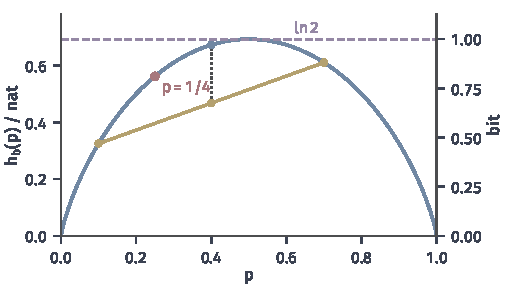
\includegraphics[width=86mm]{figures/07-probability/04-distribution-analysis/matplotlib/info-binary-entropy/figure.pdf}
  \caption{二元熵函数$h_{\mathrm{b}}(p)$（蓝），左轴nat、右轴bit。紫虚线为上界$\ln2$，在$p=\tfrac12$处达到。黄色弦连接$p=0.1$与$p=0.7$两点，其中点$0.470$低于曲线在$p=0.4$处的值$0.673$，体现凹性。红点为$p=\tfrac14$。}
  \label{fig:info-binary-entropy}
\end{BookInlineFigure}

图~\ref{fig:info-binary-entropy}中，$h_{\mathrm{b}}$在两端为零，对应确定的结果；在$p=\tfrac12$处取最大值$\ln2$，对应公平硬币；曲线关于$p=\tfrac12$对称，因为交换$0$与$1$不改变熵。端点附近曲线很陡：$h_{\mathrm{b}}'(p)=\ln\frac{1-p}{p}\to+\infty$（$p\downarrow0$），概率从$0$略微增加，熵增加得比概率快得多。第~\ref{sec:info-continuity}节讨论熵的连续性时会用到这一点。

三个取值的情形可以画在概率单纯形上。图~\ref{fig:info-simplex-entropy}中三角形的每个点是一张概率表，顶点是确定结果，中心是均匀分布。等熵线围绕中心形成一圈圈闭曲线：越靠近中心越不确定。

\begin{BookInlineFigure}
  \centering
  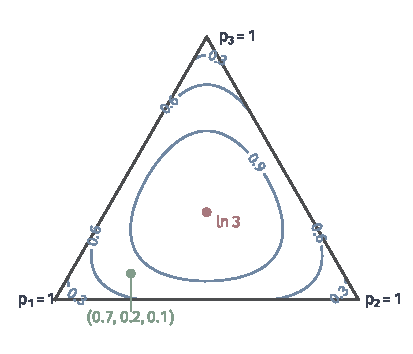
\includegraphics[width=70mm]{figures/07-probability/04-distribution-analysis/matplotlib/info-simplex-entropy/figure.pdf}
  \caption{三点分布$(p_1,p_2,p_3)$的熵在概率单纯形上的等值线（蓝，数值为nat）。顶点熵为$0$，红点为均匀分布，熵$\ln3\approx1.099$；绿点为$(0.7,0.2,0.1)$，熵约$0.802$ nat。超水平集$\{H\geq c\}$是凸集，对应熵的凹性。}
  \label{fig:info-simplex-entropy}
\end{BookInlineFigure}

\paragraph{可数取值}
取值可数无穷时，式~\eqref{eq:info-entropy}是非负项级数，可能收敛，也可能发散。几何分布$\operatorname{Geom}(\tfrac12)$取值$k=1,2,\dots$，概率$2^{-k}$，自信息$k\ln2$，于是
\[
  H(X)=\sum_{k\geq1}2^{-k}\,k\ln2=2\ln2,
\]
相当于平均问两题。

熵也可以是无穷。取$k\geq2$，$p_X(k)=c/(k(\ln k)^2)$，其中$c$使概率之和为$1$；由积分判别法，$\sum_{k\geq2}1/(k(\ln k)^2)$收敛，所以这样的$c>0$存在。这时
\[
  -\ln p_X(k)=\ln k+2\ln\ln k-\ln c\geq\ln k-\ln c.
\]
对充分大的$k$，$2\ln\ln k\geq0$，所以熵的级数从某项起不小于
\[
  \sum_k\frac{c}{k(\ln k)^2}\bigl(\ln k-\ln c\bigr)\geq\sum_k\frac{c}{k\ln k}-\ln c\sum_k\frac{c}{k(\ln k)^2},
\]
其中第一项发散，第二项有限，故$H(X)=+\infty$。这个分布的质量衰减得足够快，使概率之和有限，却不够快，使平均自信息有限。

所以定理~\ref{thm:info-entropy-range}的上界不能移用到可数字母表：$\ln m$随$m\to\infty$趋于无穷，并不给出有限上界。凹性在熵有限的分布之间仍然成立，因为证明只用到逐项的不等式；但涉及熵之差的公式，都要先核对相关的熵有限。

\subsection{微分熵}
\label{sec:info-differential-entropy}

连续随机变量的每个取值概率都是零，自信息全是无穷大，式~\eqref{eq:info-entropy}不能直接用。一个自然的替代是把概率质量换成密度：密度是单位长度上的概率质量，对密度取负对数再按分布平均。

\begin{definition}[微分熵]
\label{def:info-differential-entropy}
设随机变量$X$有密度$f_X$。若$f_X\ln f_X$在$\mathbb{R}$上可积，称
\begin{equation}
  h(X)=-\int_{\mathbb{R}}f_X(x)\ln f_X(x)\,\mathrm{d}x=\mathbb{E}[-\ln f_X(X)]
  \label{eq:info-differential-entropy}
\end{equation}
为$X$的\term{微分熵}（differential entropy），在$\{f_X=0\}$上约定被积函数为$0$。随机向量$\bm{X}$有联合密度时，同样定义$h(\bm{X})$。
\end{definition}

定义里要求$f_X\ln f_X$可积（即$f_X\lvert\ln f_X\rvert$的积分有限），是为了排除两种情形。离散熵的各项非负，最坏只是$+\infty$；而密度可以大于$1$，$-\ln f_X$有正有负，正部与负部的积分可能都发散，这时“$\infty-\infty$”没有意义。若只有一部分发散，可以约定$h(X)=+\infty$或$-\infty$，本章不使用这种扩展。

\paragraph{几个密度的微分熵}
均匀分布$\operatorname{Unif}(0,a)$的密度在$(0,a)$上为$1/a$，所以
\[
  h(X)=-\int_0^a\frac1a\ln\frac1a\,\mathrm{d}x=\ln a.
\]
$a<1$时它是负数。$\operatorname{Unif}(0,\tfrac12)$的微分熵是$-\ln2$，这不意味着“不确定性为负”，而是说密度$2$大于$1$。

正态分布$\mathcal{N}(\mu,\sigma^{2})$的对数密度是
\[
  \ln f_X(x)=-\frac12\ln(2\pi\sigma^{2})-\frac{(x-\mu)^{2}}{2\sigma^{2}}.
\]
取负号再按$X$平均，利用$\mathbb{E}[(X-\mu)^{2}]=\sigma^{2}$，得到
\begin{equation}
  h(X)=\frac12\ln(2\pi\sigma^{2})+\frac12=\frac12\ln(2\pi\mathrm{e}\sigma^{2}).
  \label{eq:info-gaussian-entropy}
\end{equation}
$\sigma=1$时约为$1.419$ nat。同样算出指数分布$\operatorname{Exp}(\lambda)$的微分熵：$-\ln f_X(x)=-\ln\lambda+\lambda x$，平均为$1-\ln\lambda$。

\paragraph{坐标尺度的作用}
把变量放大，密度就按比例变矮。设$a\neq0$，$Y=aX+b$，由第~\ref{chap:random-variable-transformations}章的换元公式，$f_Y(y)=f_X((y-b)/a)/\lvert a\rvert$。于是
\[
  -\ln f_Y(Y)=-\ln f_X(X)+\ln\lvert a\rvert,
\]
两边取期望，得到
\begin{equation}
  h(aX+b)=h(X)+\ln\lvert a\rvert.
  \label{eq:info-differential-entropy-scale}
\end{equation}
平移不改变微分熵，伸缩改变$\ln\lvert a\rvert$。图~\ref{fig:info-diff-entropy-scale}把这一点画了出来：宽度每加倍，高度减半，微分熵增加$\ln2$。

\begin{BookInlineFigure}
  \centering
  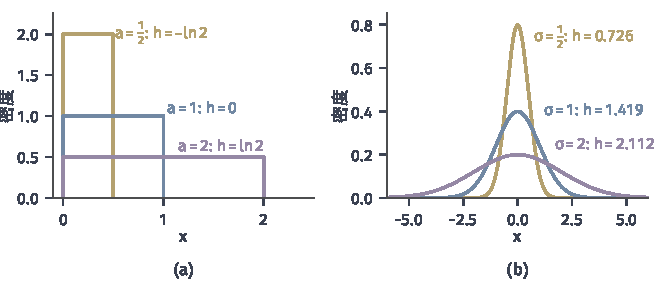
\includegraphics[width=112mm]{figures/07-probability/04-distribution-analysis/matplotlib/info-diff-entropy-scale/figure.pdf}
  \caption{微分熵随尺度变化。(a)$\operatorname{Unif}(0,a)$，$a=\tfrac12,1,2$（黄、蓝、紫），微分熵为$\ln a$。(b)$\mathcal{N}(0,\sigma^{2})$，$\sigma=\tfrac12,1,2$，微分熵按式~\eqref{eq:info-gaussian-entropy}计算，以nat计。宽度加倍时两组都增加$\ln2\approx0.693$。}
  \label{fig:info-diff-entropy-scale}
\end{BookInlineFigure}

式~\eqref{eq:info-differential-entropy-scale}揭示了微分熵与离散熵的根本不同。同一个长度用米记录是$X$，用厘米记录是$100X$，两者包含的关于这次测量的信息完全一样，微分熵却相差$\ln100$。离散熵没有这个问题：对取值作任何一一变换，概率表不变，熵不变。微分熵依赖坐标，只有在固定坐标下比较才有意义。更一般地，对严格单调可微的$g$，$Y=g(X)$满足$h(Y)=h(X)+\mathbb{E}[\ln\lvert g'(X)\rvert]$（右端各项有限时），推导与上面相同。

\paragraph{与量化后离散熵的关系}
微分熵可以从离散熵得到，只是要减去一个随精度增长的量。把实轴按宽度$\Delta>0$分成格子$[k\Delta,(k+1)\Delta)$，只记录$X$落在哪一格，得到离散变量$X_{\Delta}$，概率$p_k=\mathbb{P}(k\Delta\leq X<(k+1)\Delta)$。

若$f_X$连续，由积分中值定理，每格中有一点$\xi_k$使$p_k=f_X(\xi_k)\Delta$。代入离散熵并利用$\sum_kp_k=1$，得到
\[
  H(X_{\Delta})=-\sum_kf_X(\xi_k)\Delta\ln f_X(\xi_k)-\ln\Delta.
\]
右端第一项是$-\int f_X\ln f_X\,\mathrm{d}x$的一个Riemann和。若这个和在$\Delta\to0$时收敛到积分，就有
\begin{equation}
  H(X_{\Delta})+\ln\Delta\to h(X),\qquad\Delta\to0.
  \label{eq:info-quantized-entropy}
\end{equation}

$-\ln\Delta$是“把结果确定到精度$\Delta$”的代价：每把格子缩小一半，就要多回答一个是非题。连续结果要完全确定需要无穷多个是非题，离散熵趋于无穷；微分熵是减去这部分以后剩下的有限部分，所以它依赖格子的单位。$X\sim\operatorname{Unif}(0,1)$、$\Delta=1/n$时，$n$个格子等概率，$H(X_{\Delta})=\ln n$恰好等于$h(X)-\ln\Delta=0+\ln n$。

\begin{BookInlineFigure}
  \centering
  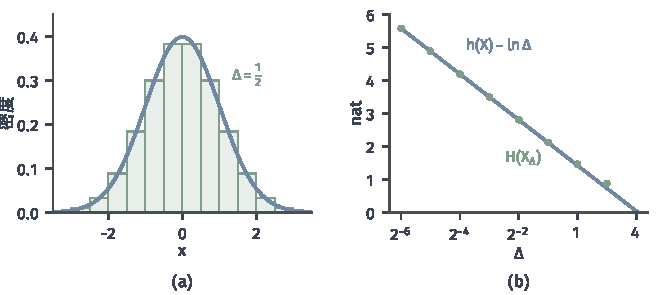
\includegraphics[width=112mm]{figures/07-probability/04-distribution-analysis/matplotlib/info-quantization/figure.pdf}
  \caption{标准正态变量的量化。(a)密度（蓝）与$\Delta=\tfrac12$时各格的概率除以格宽（浅绿柱）。(b)量化后离散熵$H(X_{\Delta})$的精确值（绿点）与$h(X)-\ln\Delta$（蓝线），$h(X)\approx1.419$ nat，横轴为对数刻度。差$H(X_{\Delta})+\ln\Delta-h(X)$在$\Delta=1,\tfrac12,\tfrac14$时约为$0.040,0.010,0.0026$。}
  \label{fig:info-quantization}
\end{BookInlineFigure}

图~\ref{fig:info-quantization}对标准正态变量逐格计算了$H(X_{\Delta})$。格子较宽时两者有可见的差距，$\Delta$每减半，差距约缩小为四分之一。

式~\eqref{eq:info-quantized-entropy}不是对任意密度都成立。上面的推导用到两件事：$f_X\ln f_X$的Riemann和收敛到积分，以及实轴无界时尾部格子的贡献可以忽略。密度连续且$f_X\ln f_X$在有界区间上Riemann可积时，有界区间上的部分成立；无界区间还需要控制尾部，读者可查阅~\scite{math-cover2006information}。密度剧烈振荡或尾部很重时，两边可能不相符。因此，微分熵与量化熵是两个不同的量，前者不是后者的极限值，而是后者减去$-\ln\Delta$后的极限，并且这个联系要单独核对条件。


\section{联合熵与条件熵}
\label{sec:info-joint-conditional}

有两个变量$X,Y$时，可以问两种问题：把有序对$(X,Y)$一起确定，平均要多少信息；已经知道$Y$以后，确定$X$还需要多少信息。前者只要把$(X,Y)$看成一个随机对象，后者要用条件分布。本节先分别定义这两个量，再说明它们怎样由“先揭示一个、再揭示另一个”的分解连接起来。

\subsection{联合熵}
\label{sec:info-joint-entropy}

有序对$(X,Y)$本身是一个离散随机对象，取值于$\mathcal{X}\times\mathcal{Y}$，联合概率质量$p_{X,Y}(x,y)$构成一张概率表。熵只依赖概率表，所以可以直接套用式~\eqref{eq:info-entropy}。

\begin{definition}[联合熵]
\label{def:info-joint-entropy}
离散随机变量$X,Y$的\term{联合熵}（joint entropy）是
\begin{equation}
  H(X,Y)=-\sum_{x,y}p_{X,Y}(x,y)\ln p_{X,Y}(x,y)=\mathbb{E}[-\ln p_{X,Y}(X,Y)].
  \label{eq:info-joint-entropy}
\end{equation}
多个变量的联合熵$H(X_1,\dots,X_n)$同样定义。若$(X,Y)$有联合密度$f_{X,Y}$，在$f_{X,Y}\lvert\ln f_{X,Y}\rvert$可积时，联合微分熵$h(X,Y)$定义为$-\iint f_{X,Y}\ln f_{X,Y}\,\mathrm{d}x\,\mathrm{d}y$。
\end{definition}

联合熵并不由两个边缘分布决定。图~\ref{fig:info-same-marginals}的三张表，$X$与$Y$的边缘都是公平硬币，$H(X)=H(Y)=\ln2$。独立时四格各$\tfrac14$，联合熵是$\ln4\approx1.386$ nat，正好是$H(X)+H(Y)$。$Y=X$时只有对角线两格有质量，联合熵只有$\ln2$：知道$X$就知道$Y$，有序对并不比单个变量更难确定。第三张表是公平硬币经过以概率$\tfrac14$出错的线路，
\[
  H(X,Y)=-2\cdot\tfrac38\ln\tfrac38-2\cdot\tfrac18\ln\tfrac18\approx1.255\ \mathrm{nat},
\]
介于前两者之间。

\begin{BookInlineFigure}
  \centering
  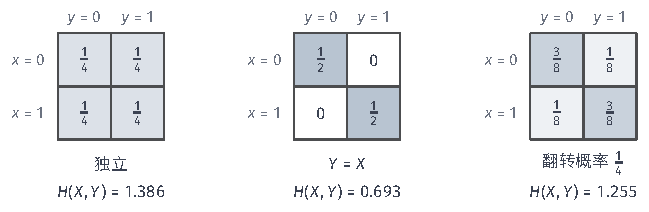
\includegraphics[width=109.8mm]{figures/07-probability/04-distribution-analysis/tikz/info-same-marginals/figure.pdf}
  \caption{三张边缘都是$(\tfrac12,\tfrac12)$的联合概率表，格中数值为$p_{X,Y}(x,y)$，底色越深质量越大。联合熵（nat）随依赖关系改变：独立时最大，$Y=X$时最小，以概率$\tfrac14$翻转时居中。}
  \label{fig:info-same-marginals}
\end{BookInlineFigure}

三张表的共同点是$H(X,Y)\leq H(X)+H(Y)$，独立时取等号；这个不等式在第~\ref{sec:info-mi-entropy}节证明。它说明依赖关系只会让整体更容易确定：一部分不确定性被两个变量“共享”了，不必重复计算。

联合微分熵的例子是二元正态分布。若$\bm{X}\sim\mathcal{N}(\bm{\mu},\bm{\Sigma})$是$d$维正态向量，协方差矩阵$\bm{\Sigma}$正定，对数密度为
\[
  \ln f(\bm{x})=-\frac12\ln\bigl((2\pi)^{d}\det\bm{\Sigma}\bigr)-\frac12(\bm{x}-\bm{\mu})^{\top}\bm{\Sigma}^{-1}(\bm{x}-\bm{\mu}).
\]
二次型的期望是$\operatorname{tr}(\bm{\Sigma}^{-1}\bm{\Sigma})=d$，所以
\begin{equation}
  h(\bm{X})=\frac12\ln\bigl((2\pi\mathrm{e})^{d}\det\bm{\Sigma}\bigr).
  \label{eq:info-gaussian-vector-entropy}
\end{equation}
二维标准化、相关系数为$\rho$时$\det\bm{\Sigma}=1-\rho^{2}$，相关越强，联合微分熵越小，$\lvert\rho\rvert\to1$时趋于$-\infty$。质量越来越集中到一条直线附近，平面上的密度越来越高。

\subsection{条件熵}
\label{sec:info-conditional-entropy}

已知$Y=y$以后，$X$的概率表变成条件分布$p_{X\mid Y}(\cdot\mid y)$：条件化就是只保留$Y=y$的那一列，再重新归一。这张新表的熵，是看到$Y=y$以后$X$剩下的不确定性。不同的$y$留下的不确定性不同，再按$y$出现的概率平均。

\begin{definition}[条件熵]
\label{def:info-conditional-entropy}
设$X,Y$是离散随机变量。对$p_Y(y)>0$的$y$，令
\begin{equation}
  H(X\mid Y=y)=-\sum_xp_{X\mid Y}(x\mid y)\ln p_{X\mid Y}(x\mid y).
  \label{eq:info-conditional-entropy-value}
\end{equation}
$X$在给定$Y$时的\term{条件熵}（conditional entropy）是
\begin{equation}
  H(X\mid Y)=\sum_{y}p_Y(y)\,H(X\mid Y=y)=\mathbb{E}\bigl[-\ln p_{X\mid Y}(X\mid Y)\bigr].
  \label{eq:info-conditional-entropy}
\end{equation}
\end{definition}

式~\eqref{eq:info-conditional-entropy}中第一个和是对式~\eqref{eq:info-conditional-entropy-value}的平均。第二个等号把双重求和合并：$p_Y(y)p_{X\mid Y}(x\mid y)=p_{X,Y}(x,y)$，所以
\[
  H(X\mid Y)=-\sum_{x,y}p_{X,Y}(x,y)\ln p_{X\mid Y}(x\mid y),
\]
各项非负，求和次序可以交换。条件熵是平均剩余不确定性，不是对某一个观测值的保证。

\paragraph{一张不对称的表}
下面这张表在后面几节反复使用：
\begin{equation}
  p_{X,Y}(0,0)=\tfrac14,\quad p_{X,Y}(0,1)=0,\quad p_{X,Y}(1,0)=\tfrac38,\quad p_{X,Y}(1,1)=\tfrac38.
  \label{eq:info-z-table}
\end{equation}
可以把它想成：$X=0$时$Y$必为$0$；$X=1$时$Y$是一枚公平硬币。边缘分布为
\[
  p_X=(\tfrac14,\tfrac34),\qquad p_Y=(\tfrac58,\tfrac38).
\]

按行看，$X=0$那一行条件分布是$(1,0)$，熵为$0$；$X=1$那一行是$(\tfrac12,\tfrac12)$，熵为$\ln2$。按$p_X$平均，
\[
  H(Y\mid X)=\tfrac14\cdot0+\tfrac34\ln2\approx0.520\ \mathrm{nat}.
\]

按列看，$Y=0$那一列的条件分布是$(\tfrac14,\tfrac38)/\tfrac58=(\tfrac25,\tfrac35)$，熵为$h_{\mathrm{b}}(\tfrac25)\approx0.673$；$Y=1$那一列是$(0,1)$，熵为$0$。按$p_Y$平均，
\[
  H(X\mid Y)=\tfrac58\cdot0.673+\tfrac38\cdot0\approx0.421\ \mathrm{nat}.
\]
两个条件熵不相等：条件熵与“谁给定谁”有关。

\begin{BookInlineFigure}
  \centering
  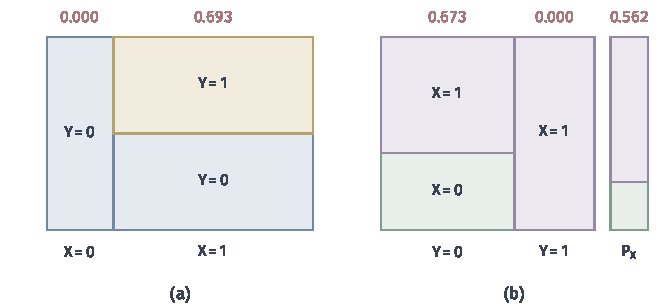
\includegraphics[width=112mm]{figures/07-probability/04-distribution-analysis/matplotlib/info-conditional-slices/figure.pdf}
  \caption{表~\eqref{eq:info-z-table}的条件分布。(a)按$X$分割，宽度为$p_X(x)$，高度为$Y$的条件概率，红色数字为各行的条件熵$H(Y\mid X=x)$。(b)按$Y$分割，宽度正比于$p_Y(y)$，高度为$X$的条件概率，红色数字为$H(X\mid Y=y)$；最右的窄条是无条件的$p_X$及其熵$H(X)\approx0.562$。单位为nat。}
  \label{fig:info-conditional-slices}
\end{BookInlineFigure}

图~\ref{fig:info-conditional-slices}(b)还显示了一个容易误解的现象：$H(X\mid Y=0)\approx0.673$大于$H(X)\approx0.562$。观测到$Y=0$以后，$X$反而更不确定了，因为$Y=0$把原来偏向$X=1$的质量拉向均匀。但这样的观测值只是一部分；$Y=1$时$X$完全确定。平均以后$H(X\mid Y)\approx0.421$，仍小于$H(X)$。第~\ref{sec:info-mi-entropy}节证明这对一切离散变量成立：条件化平均来说不增加熵，但单个观测值可以增加。

\paragraph{离散与连续的区别}
离散时$H(X\mid Y=y)\geq0$，所以$H(X\mid Y)\geq0$，等号当且仅当每个$y$下$X$确定，即$X$是$Y$的函数（除去零概率的$y$）。连续时用条件密度代替条件概率，定义
\[
  h(X\mid Y)=-\iint f_{X,Y}(x,y)\ln f_{X\mid Y}(x\mid y)\,\mathrm{d}x\,\mathrm{d}y,
\]
要求条件密度存在且被积函数绝对可积。它和微分熵一样可以为负，也依赖坐标。

二元标准正态、相关系数$\rho$时，给定$X=x$，$Y$的条件分布是$\mathcal{N}(\rho x,1-\rho^{2})$，与$x$有关的只有均值。每个条件分布的微分熵相同，由式~\eqref{eq:info-gaussian-entropy}，
\begin{equation}
  h(Y\mid X)=\frac12\ln\bigl(2\pi\mathrm{e}(1-\rho^{2})\bigr).
  \label{eq:info-gaussian-conditional-entropy}
\end{equation}
$\rho=0.9$时它约为$0.589$ nat；$\rho^{2}>1-1/(2\pi\mathrm{e})\approx0.941$时它为负数。负值只说明条件密度很窄，不能读成“剩余不确定性为负”。

\subsection{熵的链式法则}
\label{sec:info-entropy-chain-rule}

确定$(X,Y)$可以分两步：先确定$X$，再在已知$X$的情况下确定$Y$。图~\ref{fig:info-chain-tree}把表~\eqref{eq:info-z-table}画成两步的树。第一步的不确定性是$H(X)\approx0.562$；第二步要看走到哪一支，$X=0$那支已无悬念，$X=1$那支还剩$\ln2$，平均$0.520$。两步合起来应当是整体的不确定性。

\begin{BookInlineFigure}
  \centering
  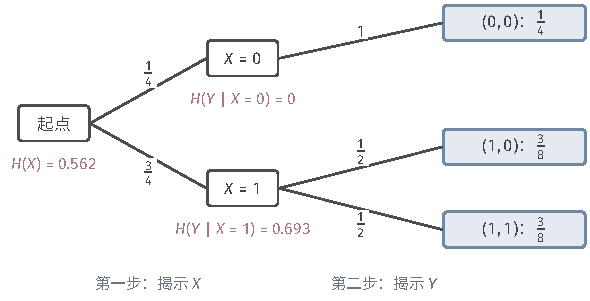
\includegraphics[width=100mm]{figures/07-probability/04-distribution-analysis/tikz/info-chain-tree/figure.pdf}
  \caption{表~\eqref{eq:info-z-table}的两步揭示树。第一步按$p_X=(\tfrac14,\tfrac34)$揭示$X$，第二步按条件分布揭示$Y$；叶子为联合概率。红字为各步的熵（nat），第二步的平均为$\tfrac34\ln2\approx0.520$，与第一步的$0.562$相加得$H(X,Y)\approx1.082$。}
  \label{fig:info-chain-tree}
\end{BookInlineFigure}

\begin{theorem}[熵的链式法则]
\label{thm:info-entropy-chain-rule}
设$X,Y$是离散随机变量，则在$[0,\infty]$中
\begin{equation}
  H(X,Y)=H(X)+H(Y\mid X).
  \label{eq:info-entropy-chain-rule}
\end{equation}
对离散随机变量$X_1,\dots,X_n$，
\begin{equation}
  H(X_1,\dots,X_n)=\sum_{i=1}^{n}H(X_i\mid X_1,\dots,X_{i-1}),
  \label{eq:info-entropy-chain-rule-n}
\end{equation}
其中$i=1$的项理解为$H(X_1)$。
\end{theorem}

\begin{proof}
在$p_{X,Y}(x,y)>0$的点，$p_{X,Y}(x,y)=p_X(x)\,p_{Y\mid X}(y\mid x)$，取负对数，得到
\[
  -\ln p_{X,Y}(x,y)=-\ln p_X(x)-\ln p_{Y\mid X}(y\mid x).
\]
右端两项都非负。乘以$p_{X,Y}(x,y)$后对$(x,y)$求和；非负项的和可以拆开、可以交换次序，即使为$+\infty$也成立。第一项的和是$-\sum_xp_X(x)\ln p_X(x)=H(X)$，第二项的和由式~\eqref{eq:info-conditional-entropy}是$H(Y\mid X)$。

多个变量时，把$(X_1,\dots,X_{n-1})$看成一个变量，对它与$X_n$用式~\eqref{eq:info-entropy-chain-rule}，得到
\[
  H(X_1,\dots,X_n)=H(X_1,\dots,X_{n-1})+H(X_n\mid X_1,\dots,X_{n-1}),
\]
再对前一项归纳即可。
\end{proof}

用表~\eqref{eq:info-z-table}验证。直接计算联合熵，
\[
  H(X,Y)=-\tfrac14\ln\tfrac14-2\cdot\tfrac38\ln\tfrac38\approx1.082.
\]
先揭示$X$，$H(X)+H(Y\mid X)\approx0.562+0.520=1.082$。换一个顺序，$H(Y)=h_{\mathrm{b}}(\tfrac38)\approx0.662$，$H(Y)+H(X\mid Y)\approx0.662+0.421=1.082$，也相同。揭示的顺序不同，每一步分到的不确定性不同，总量不变。

链式法则不要求独立。变量独立时，$p_{X_i\mid X_1,\dots,X_{i-1}}=p_{X_i}$，各条件熵等于无条件熵，式~\eqref{eq:info-entropy-chain-rule-n}化为$\sum_iH(X_i)$。不独立时不能把联合熵写成边缘熵之和，图~\ref{fig:info-same-marginals}已经给出了反例。

\paragraph{移项与连续情形}
链式法则常被移项为$H(Y\mid X)=H(X,Y)-H(X)$。这只在$H(X)<\infty$时有意义；否则右端可能是$\infty-\infty$。例如取$H(X)=\infty$的可数变量并令$Y=X$，$H(X,Y)=\infty$，$H(Y\mid X)=0$，链式法则$\infty=\infty+0$成立，移项却没有意义。

对有联合密度的$(X,Y)$，同样有$f_{X,Y}=f_X\,f_{Y\mid X}$，取负对数后积分，得到
\[
  h(X,Y)=h(X)+h(Y\mid X).
\]
但这里各项可以为负，不能像离散时那样靠“非负项可以拆开”保证等式。需要先核对$f_X\lvert\ln f_X\rvert$与$f_{X,Y}\lvert\ln f_{Y\mid X}\rvert$都可积，这时拆开积分合法，等式成立，并且$h(X,Y)$也有限。二元正态是一个检查的例子：由式~\eqref{eq:info-gaussian-entropy}与式~\eqref{eq:info-gaussian-conditional-entropy}，
\[
  h(X)+h(Y\mid X)=\frac12\ln(2\pi\mathrm{e})+\frac12\ln\bigl(2\pi\mathrm{e}(1-\rho^{2})\bigr),
\]
与式~\eqref{eq:info-gaussian-vector-entropy}在$d=2$、$\det\bm{\Sigma}=1-\rho^{2}$时的值相同。


\section{互信息}
\label{sec:info-mutual-information}

公平硬币$X$经过以概率$\tfrac14$出错的线路得到$Y$。看到$Y$之前，$X$的不确定性是$\ln2$；看到$Y$以后，平均剩下$H(X\mid Y)=h_{\mathrm{b}}(\tfrac14)\approx0.562$。两者之差约$0.131$ nat，是观测$Y$平均消除的不确定性。这个差可以作为“$Y$含有多少关于$X$的信息”。

但熵之差只在熵有限、并且两个变量都是离散时才写得出来。连续变量的微分熵依赖坐标，一个变量离散、另一个连续时还会出现某一项根本没有定义的情形。本节换一个出发点：$X$与$Y$不相关联，就是联合分布等于边缘分布的乘积；联合分布偏离这个乘积的程度，用KL散度衡量。这个定义对任何取值空间都有意义，熵之差是它在条件满足时的一种算法。

\subsection{定义与独立性}
\label{sec:info-mi-definition}

先回顾第~\ref{chap:distribution-comparison}章的KL散度。设$P,Q$是同一可测空间上的概率分布。若$P\ll Q$，记$r=\mathrm{d}P/\mathrm{d}Q$，则
\begin{equation}
  D_{\mathrm{KL}}(P\Vert Q)=\int\ln r\,\mathrm{d}P\in[0,+\infty];
  \label{eq:info-kl-recall}
\end{equation}
若$P$不绝对连续于$Q$，则$D_{\mathrm{KL}}(P\Vert Q)=+\infty$。$\ln r$的负部总对$P$可积，所以积分总有意义；KL散度非负，并且为零当且仅当$P=Q$。离散时$r(x)=p(x)/q(x)$，式~\eqref{eq:info-kl-recall}化为$\sum_xp(x)\ln\frac{p(x)}{q(x)}$。

\begin{definition}[互信息]
\label{def:info-mutual-information}
设随机变量（或随机元素）$X,Y$的联合分布为$P_{X,Y}$，边缘分布为$P_X,P_Y$。$X$与$Y$的\term{互信息}（mutual information）是
\begin{equation}
  I(X;Y)=D_{\mathrm{KL}}\bigl(P_{X,Y}\Vert P_X\otimes P_Y\bigr)\in[0,+\infty].
  \label{eq:info-mutual-information}
\end{equation}
离散时
\begin{equation}
  I(X;Y)=\sum_{x,y}p_{X,Y}(x,y)\ln\frac{p_{X,Y}(x,y)}{p_X(x)\,p_Y(y)}.
  \label{eq:info-mutual-information-discrete}
\end{equation}
\end{definition}

$P_X\otimes P_Y$是“边缘不变、但把两个变量拆成独立”所得的分布。互信息比较真实的联合规律与这个独立参照，差异全部来自依赖关系，因为两者的边缘完全相同。

\begin{theorem}[互信息的基本性质]
\label{thm:info-mi-basic}
对任意随机元素$X,Y$：
\begin{enumerate}
  \item $I(X;Y)\geq0$；
  \item $I(X;Y)=I(Y;X)$；
  \item $I(X;Y)=0$当且仅当$X$与$Y$独立。
\end{enumerate}
\end{theorem}

\begin{proof}
第一条和第三条是KL散度的非负性及其零值条件：$I(X;Y)=0$当且仅当$P_{X,Y}=P_X\otimes P_Y$，而这正是第~\ref{chap:probability-spaces}章中独立的定义。

第二条用交换坐标的映射$\sigma(x,y)=(y,x)$。它把$P_{X,Y}$推前为$P_{Y,X}$，把$P_X\otimes P_Y$推前为$P_Y\otimes P_X$。若$P_{X,Y}\ll P_X\otimes P_Y$，密度为$r$，则$r\circ\sigma^{-1}$是推前后两个分布之间的密度，按推前测度的积分换元，两个KL的积分相等；若不绝对连续，推前后同样不绝对连续，两边都是$+\infty$。
\end{proof}

第三条比“协方差为零”强得多。取$X$在$\{-1,0,1\}$上均匀，$Y=X^{2}$：$\operatorname{Cov}(X,Y)=\mathbb{E}[X^{3}]=0$，但$Y$由$X$确定，下一小节会算出$I(X;Y)\approx0.637>0$。互信息为零能排除一切形式的依赖，零协方差只能排除线性部分。

\paragraph{二元例子}
用式~\eqref{eq:info-mutual-information-discrete}计算出错线路的例子。联合表是对角$\tfrac38$、非对角$\tfrac18$，边缘乘积处处$\tfrac14$，比值分别为$\tfrac32$与$\tfrac12$。于是
\[
  I(X;Y)=2\cdot\tfrac38\ln\tfrac32+2\cdot\tfrac18\ln\tfrac12=\tfrac34\ln\tfrac32-\tfrac14\ln2\approx0.1308\ \mathrm{nat},
\]
约$0.189$ bit。对角格的比值大于$1$，说明“相同”比独立时更常见；非对角格的比值小于$1$，对数为负，但按$P_{X,Y}$加权后总和非负。

\paragraph{互信息可以为无穷}
定义允许$I(X;Y)=+\infty$，这不是边缘情形。设$X\sim\operatorname{Unif}(0,1)$，$Y=X$。联合分布全部集中在对角线$D=\{(x,x)\}$上，$P_{X,Y}(D)=1$；而
\[
  (P_X\otimes P_Y)(D)=\int_0^1P_Y(\{x\})\,\mathrm{d}x=0.
\]
$P_{X,Y}$不绝对连续于$P_X\otimes P_Y$，所以$I(X;Y)=+\infty$。一个连续变量完全知道另一个连续变量，等于知道了无穷多位小数。离散时也会出现无穷：若$H(X)=+\infty$，令$Y=X$，下一小节会得到$I(X;Y)=H(X)=+\infty$。

定义也不要求任何密度。联合分布可以没有联合密度，比如上面集中在对角线上的分布；只要$P_{X,Y}\ll P_X\otimes P_Y$，KL就由密度比计算，否则直接为无穷。

\subsection{与熵的关系}
\label{sec:info-mi-entropy}

回到章首的说法：互信息是观测带来的不确定性的减少。下面的定理说明，离散情形下只要相关的熵有限，两种说法一致。

\begin{theorem}[互信息与熵]
\label{thm:info-mi-entropy}
设$X,Y$是离散随机变量。若$H(X)<\infty$，则$H(X\mid Y)\leq H(X)$，并且
\begin{equation}
  I(X;Y)=H(X)-H(X\mid Y).
  \label{eq:info-mi-entropy-difference}
\end{equation}
若$H(X)$与$H(Y)$都有限，则$H(X,Y)$有限，并且
\begin{equation}
  I(X;Y)=H(X)+H(Y)-H(X,Y).
  \label{eq:info-mi-entropy-sum}
\end{equation}
\end{theorem}

\begin{proof}
在$p_{X,Y}(x,y)>0$的点，把比值中的$p_{X,Y}/p_Y$写成条件概率，
\[
  \ln\frac{p_{X,Y}(x,y)}{p_X(x)p_Y(y)}=\bigl(-\ln p_X(x)\bigr)-\bigl(-\ln p_{X\mid Y}(x\mid y)\bigr).
\]
记$A=-\ln p_X(X)$，$B=-\ln p_{X\mid Y}(X\mid Y)$。两者非负，期望分别为
\[
  \mathbb{E}[A]=H(X)<\infty,\qquad\mathbb{E}[B]=H(X\mid Y).
\]由式~\eqref{eq:info-mutual-information-discrete}，$I(X;Y)=\mathbb{E}[A-B]$。$A$可积而$B\geq0$，期望可以拆开，得到
\[
  I(X;Y)=\mathbb{E}[A]-\mathbb{E}[B]=H(X)-H(X\mid Y).
\]
互信息非负，所以$H(X\mid Y)\leq H(X)$，右端是两个有限数之差。

第二个等式由链式法则得到：$H(Y)<\infty$时由第一部分$H(X\mid Y)\leq H(X)<\infty$，式~\eqref{eq:info-entropy-chain-rule}给出$H(X,Y)=H(Y)+H(X\mid Y)$有限，代入式~\eqref{eq:info-mi-entropy-difference}即得。
\end{proof}

由对称性，同样有$I(X;Y)=H(Y)-H(Y\mid X)$（$H(Y)<\infty$时）。这几个关系有三个直接推论，都在相应熵有限时成立：
\begin{itemize}
  \item \textbf{条件化平均不增加熵}：$H(X\mid Y)\leq H(X)$，等号当且仅当$X,Y$独立。上一节的表~\eqref{eq:info-z-table}说明，这个结论只对平均成立，对单个观测值$H(X\mid Y=0)$可以大于$H(X)$。
  \item \textbf{联合熵的次可加性}：$H(X,Y)\leq H(X)+H(Y)$，这正是图~\ref{fig:info-same-marginals}中观察到的。
  \item \textbf{上界}：$I(X;Y)\leq\min\{H(X),H(Y)\}$，并且$I(X;X)=H(X)$，因为$H(X\mid X)=0$。离散变量与自身的互信息就是它的熵，熵因此也叫“自身信息”。
\end{itemize}

$Y=X^{2}$的例子中，$Y$是$X$的函数，$H(Y\mid X)=0$，所以$I(X;Y)=H(Y)$；$Y$取$1$的概率是$\tfrac23$，$H(Y)=h_{\mathrm{b}}(\tfrac13)\approx0.637$。

\begin{BookInlineFigure}
  \centering
  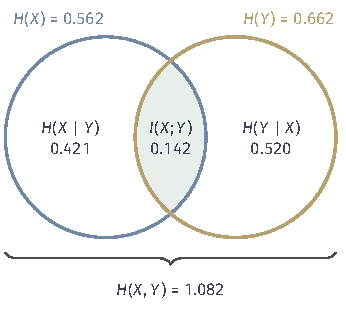
\includegraphics[width=58.5mm]{figures/07-probability/04-distribution-analysis/tikz/info-venn/figure.pdf}
  \caption{两个离散变量的熵与互信息的记账图，数值（nat）取自表~\eqref{eq:info-z-table}。蓝圈表示$H(X)$，黄圈表示$H(Y)$，重叠部分（浅绿）表示$I(X;Y)$，两圈之外的部分分别是条件熵，两圈的并表示$H(X,Y)$。图只表示有限熵之间的加减关系，面积不是测度。}
  \label{fig:info-venn}
\end{BookInlineFigure}

图~\ref{fig:info-venn}把这些关系画成两个重叠的圆。表~\eqref{eq:info-z-table}给出
\[
  I(X;Y)=H(X)-H(X\mid Y)\approx0.562-0.421=0.142,
\]
也等于$H(Y)-H(Y\mid X)\approx0.662-0.520=0.142$。图很方便记忆，但它只是有限熵之间的记账：三个变量时，三圈公共部分对应的量可以为负（第~\ref{sec:info-mi-chain-rule}节的异或例子），连续变量时各块可以为负，不能把它当成真正的面积。

再看出错线路的例子随出错概率$\varepsilon$的变化。$H(X)=\ln2$不变，$H(X\mid Y)=h_{\mathrm{b}}(\varepsilon)$，所以
\[
  I(X;Y)=\ln2-h_{\mathrm{b}}(\varepsilon).
\]
图~\ref{fig:info-bsc-curves}中两条曲线之和始终是$\ln2$。$\varepsilon=0$时观测完全揭示$X$；$\varepsilon=\tfrac12$时$Y$与$X$独立，互信息为零；$\varepsilon=1$时线路总是出错，把$Y$翻转回来就完全知道$X$，互信息又回到$\ln2$。互信息衡量的是能否从$Y$推出$X$，不是$Y$与$X$是否相等。

\begin{BookInlineFigure}
  \centering
  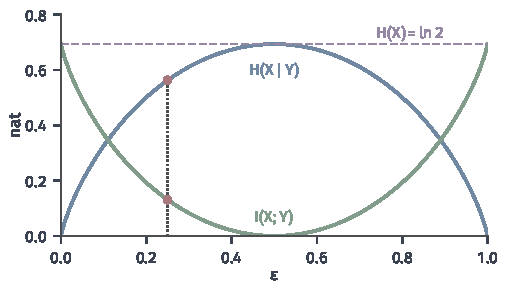
\includegraphics[width=86mm]{figures/07-probability/04-distribution-analysis/matplotlib/info-bsc-curves/figure.pdf}
  \caption{公平硬币$X$经以概率$\varepsilon$出错的线路得到$Y$。蓝线为$H(X\mid Y)=h_{\mathrm{b}}(\varepsilon)$，绿线为$I(X;Y)=\ln2-h_{\mathrm{b}}(\varepsilon)$，紫虚线为$H(X)=\ln2$，单位nat。红点为$\varepsilon=\tfrac14$：$0.562$与$0.131$。}
  \label{fig:info-bsc-curves}
\end{BookInlineFigure}

\paragraph{连续情形}
$(X,Y)$有联合密度时，若$h(Y)$与$h(Y\mid X)$都有限，同样的推导（把求和换成积分，拆开的依据是两项都绝对可积）给出
\[
  I(X;Y)=h(Y)-h(Y\mid X).
\]
二元标准正态由式~\eqref{eq:info-gaussian-entropy}与式~\eqref{eq:info-gaussian-conditional-entropy}得到
\begin{equation}
  I(X;Y)=\frac12\ln(2\pi\mathrm{e})-\frac12\ln\bigl(2\pi\mathrm{e}(1-\rho^{2})\bigr)=-\frac12\ln(1-\rho^{2}).
  \label{eq:info-gaussian-mi}
\end{equation}
$\rho=0.9$时约$0.830$ nat；$\lvert\rho\rvert\to1$时趋于无穷，与上面$Y=X$的例子一致。两个微分熵各自依赖坐标，相减后的互信息不依赖：分别把$X,Y$作伸缩，式~\eqref{eq:info-differential-entropy-scale}中的$\ln\lvert a\rvert$在两项中相消。

\begin{BookInlineFigure}
  \centering
  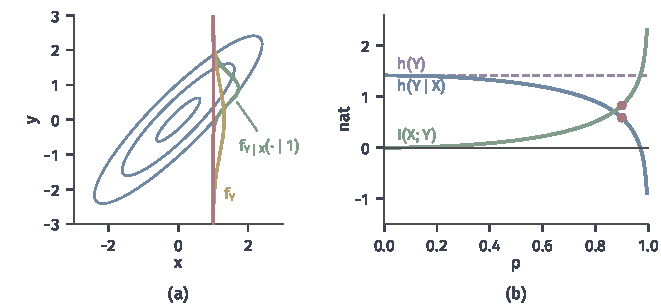
\includegraphics[width=112mm]{figures/07-probability/04-distribution-analysis/matplotlib/info-gaussian-mi/figure.pdf}
  \caption{二元标准正态分布。(a)$\rho=0.9$时联合密度的等值线（蓝）；红线为$x=1$，绿线为$Y$在$X=1$下的条件密度$\mathcal{N}(0.9,0.19)$，黄线为$Y$的边缘密度$\mathcal{N}(0,1)$，均横向画出。(b)$h(Y)$（紫虚线）、$h(Y\mid X)$（蓝）与$I(X;Y)$（绿）随$\rho$的变化，单位nat；红点为$\rho=0.9$时的$0.589$与$0.830$。}
  \label{fig:info-gaussian-mi}
\end{BookInlineFigure}

图~\ref{fig:info-gaussian-mi}(a)是熵差的直观来源：条件密度比边缘密度窄得多，宽度之比的对数就是减少的不确定性。(b)中$h(Y\mid X)$在$\rho$接近$1$时变为负数，而互信息始终非负。

熵差公式需要的熵可能不存在，互信息却仍有定义。设$X$等可能取$\pm1$，$Z\sim\mathcal{N}(0,1)$与$X$独立，$Y=X+Z$。$X$是离散的，没有密度，$h(X)$与$h(X\mid Y)$都没有定义，“$h(X)-h(X\mid Y)$”写不出来。但给定$X=x$时$Y$的条件密度是$\varphi(y-x)$，$h(Y\mid X)=\tfrac12\ln(2\pi\mathrm{e})$；$Y$的密度是两个正态密度的平均，方差为$2$，$h(Y)$有限。于是
\[
  I(X;Y)=h(Y)-h(Y\mid X)
\]
是一个有限的正数。所以，熵差是在各项有意义时计算互信息的工具，而式~\eqref{eq:info-mutual-information}才是定义。

\subsection{条件互信息}
\label{sec:info-conditional-mi}

已经知道第三个变量$Z$时，$X$与$Y$之间还剩多少共享信息？做法与条件熵相同：固定$Z=z$，在条件分布下计算互信息，再按$Z$的分布平均。连续的$Z$要用第~\ref{chap:conditional-distributions}章的正则条件分布，才能对每个$z$谈论“给定$Z=z$时$(X,Y)$的分布”。

\begin{definition}[条件互信息]
\label{def:info-conditional-mi}
设$X,Y,Z$取值于标准Borel空间，于是$(X,Y)$给定$Z$的正则条件分布$P_{X,Y\mid Z}(\cdot\mid z)$存在，记其边缘为$P_{X\mid Z}(\cdot\mid z)$、$P_{Y\mid Z}(\cdot\mid z)$。$X$与$Y$在给定$Z$时的\term{条件互信息}（conditional mutual information）是
\begin{equation}
  I(X;Y\mid Z)=\int D_{\mathrm{KL}}\bigl(P_{X,Y\mid Z}(\cdot\mid z)\Vert P_{X\mid Z}(\cdot\mid z)\otimes P_{Y\mid Z}(\cdot\mid z)\bigr)\,P_Z(\mathrm{d}z).
  \label{eq:info-conditional-mi}
\end{equation}
离散时
\begin{equation}
  I(X;Y\mid Z)=\sum_{x,y,z}p_{X,Y,Z}(x,y,z)\ln\frac{p_{X,Y\mid Z}(x,y\mid z)}{p_{X\mid Z}(x\mid z)\,p_{Y\mid Z}(y\mid z)}.
  \label{eq:info-conditional-mi-discrete}
\end{equation}
\end{definition}

被积函数是$z$的非负可测函数，积分在$[0,+\infty]$中总有意义。正则条件分布只在$P_Z$几乎处处的意义下唯一，换一个版本只在零概率的$z$上改变被积函数，积分不变。没有标准Borel这类条件时，正则条件分布可能不存在，式~\eqref{eq:info-conditional-mi}就不能这样写。

\begin{theorem}[条件互信息与条件独立]
\label{thm:info-conditional-mi-zero}
在定义~\ref{def:info-conditional-mi}的条件下，$I(X;Y\mid Z)\geq0$；$I(X;Y\mid Z)=0$当且仅当$X$与$Y$在给定$Z$时条件独立。
\end{theorem}

\begin{proof}
被积函数是KL散度，非负，所以积分非负。非负函数的积分为零，当且仅当它对$P_Z$几乎处处为零；由KL的零值条件，这就是对几乎所有$z$，
\[
  P_{X,Y\mid Z}(\cdot\mid z)=P_{X\mid Z}(\cdot\mid z)\otimes P_{Y\mid Z}(\cdot\mid z).
\]按第~\ref{chap:conditional-distributions}章，这正是给定$Z$时的条件独立。
\end{proof}

在离散且$H(X\mid Z)<\infty$时，把定理~\ref{thm:info-mi-entropy}的证明逐个条件值地做一遍，得到
\begin{equation}
  I(X;Y\mid Z)=H(X\mid Z)-H(X\mid Y,Z).
  \label{eq:info-conditional-mi-entropy}
\end{equation}
它是在已经知道$Z$的前提下，再观测$Y$所减少的关于$X$的不确定性。

条件互信息与互信息是两个不同的量，下一小节的例子说明两者之间没有固定的大小关系。

\subsection{互信息的链式法则}
\label{sec:info-mi-chain-rule}

一组观测$(Y,Z)$提供的关于$X$的信息，可以分两步获得：先看$Y$，得到$I(X;Y)$；再看$Z$，新增的是已知$Y$时$Z$还能提供的信息$I(X;Z\mid Y)$。

\begin{theorem}[互信息的链式法则]
\label{thm:info-mi-chain-rule}
设$X,Y,Z$取值于标准Borel空间，则在$[0,+\infty]$中
\begin{equation}
  I(X;Y,Z)=I(X;Y)+I(X;Z\mid Y).
  \label{eq:info-mi-chain-rule}
\end{equation}
一般地，
\begin{equation}
  I(X;Y_1,\dots,Y_n)=\sum_{i=1}^{n}I(X;Y_i\mid Y_1,\dots,Y_{i-1}).
  \label{eq:info-mi-chain-rule-n}
\end{equation}
\end{theorem}

\begin{proof}
先证离散且$H(X)<\infty$的情形。由式~\eqref{eq:info-mi-entropy-difference}及其条件形式~\eqref{eq:info-conditional-mi-entropy}，
\[
  I(X;Y,Z)=H(X)-H(X\mid Y,Z),\qquad I(X;Y)=H(X)-H(X\mid Y),
\]
以及
\[
  I(X;Z\mid Y)=H(X\mid Y)-H(X\mid Y,Z).
\]
三个式子里的熵都不超过$H(X)$，都是有限数。后两式相加，$H(X\mid Y)$相消，得到第一式。

一般情形不能假定熵有限，要直接分解KL散度。在离散情形，对一切三元组有
\[
  \frac{p_{X,Y,Z}}{p_X\,p_{Y,Z}}=\frac{p_{X,Y}}{p_X\,p_Y}\cdot\frac{p_{X,Z\mid Y}}{p_{X\mid Y}\,p_{Z\mid Y}},
\]
等式两边分子分母都按$p_{X,Y,Z}=p_{X,Y}\,p_{Z\mid X,Y}$与$p_{Y,Z}=p_Y\,p_{Z\mid Y}$展开即可核对。取对数后按$P_{X,Y,Z}$平均，第一个因子给出$I(X;Y)$，第二个给出$I(X;Z\mid Y)$。在一般空间，这一步是KL散度对联合分布的分解：两个联合分布的KL等于边缘的KL加上条件分布KL的平均。把两项的平均拆开、并允许取$+\infty$，需要用到对数比负部的可积性与正则条件分布的可测性，推导较长，这里只用它的结论。

多个观测时对$n$归纳：把$(Y_1,\dots,Y_{n-1})$看成一个变量，对它与$Y_n$用式~\eqref{eq:info-mi-chain-rule}。
\end{proof}

一般空间中KL散度分解的完整论证，读者可查阅~\scite{math-cover2006information}。

链式法则说明，信息可以按观测的先后分批记账，与熵的链式法则平行。不过，下面两个例子说明，第二步的条件互信息可以比无条件的互信息大，也可以小。

\paragraph{条件化可以增加互信息}
设$X,Y$是独立的公平硬币，$Z=X\oplus Y$为异或（相同为$0$，不同为$1$）。$X,Y$独立，$I(X;Y)=0$。给定$Z=0$时，$(X,Y)$只取$(0,0),(1,1)$，各$\tfrac12$，$Y$由$X$确定；给定$Z=1$时只取$(0,1),(1,0)$。于是
\[
  I(X;Y\mid Z)=H(X\mid Z)-H(X\mid Y,Z)=\ln2-0=\ln2.
\]
这里用到$X$与$Z$独立（$Z$在$X$的每个取值下都是公平硬币），所以$H(X\mid Z)=\ln2$；而知道$Y$与$Z$就能算出$X=Y\oplus Z$。

\begin{BookInlineFigure}
  \centering
  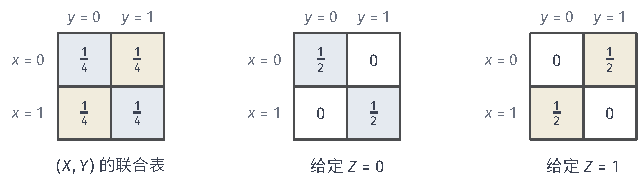
\includegraphics[width=108.6mm]{figures/07-probability/04-distribution-analysis/tikz/info-xor/figure.pdf}
  \caption{异或例子。左：独立公平硬币$(X,Y)$的联合表，蓝格$Z=X\oplus Y=0$，黄格$Z=1$。中、右：给定$Z=0$与$Z=1$后$(X,Y)$的条件表，质量只落在两格上，$Y$由$X$确定。}
  \label{fig:info-xor}
\end{BookInlineFigure}

图~\ref{fig:info-xor}给出了直观：单看$(X,Y)$，四格均匀，看不出任何关联；一旦知道$Z$，就只剩两格，$X$与$Y$紧紧绑在一起。$Z$本身不含关于$X$的信息，它提供的是$X$与$Y$之间的约束。

用链式法则从两个方向计算$I(X;Y,Z)$。先看$Y$再看$Z$：
\[
  I(X;Y)+I(X;Z\mid Y)=0+\ln2.
\]
先看$Z$再看$Y$：
\[
  I(X;Z)+I(X;Y\mid Z)=0+\ln2.
\]
两种顺序都给出$\ln2$：单独看$Y$或$Z$都毫无用处，两者合起来却完全确定$X$。

\paragraph{条件化可以减少互信息}
设$X$是公平硬币，$Y=Z=X$。则$I(X;Y)=H(X)=\ln2$；给定$Z$以后$X,Y$都已确定，$I(X;Y\mid Z)=0$。这次$Z$与$Y$携带的是同一份信息，知道$Z$以后，$Y$不再提供新东西。

两个例子放在一起说明，“三圈公共部分”$I(X;Y)-I(X;Y\mid Z)$在异或例子中等于$-\ln2$，在复制例子中等于$\ln2$。图~\ref{fig:info-venn}那样的记账图不能推广到三个变量的面积图，条件化前后的互信息要分别计算。


\section{交叉熵}
\label{sec:info-cross-entropy}

图~\ref{fig:info-question-tree}的提问方案是按真实概率$(\tfrac12,\tfrac14,\tfrac18,\tfrac18)$设计的：越常见的结果问得越少。如果设计者误以为四个字母等可能，就会给每个字母都安排两题；如果误以为概率是$(\tfrac18,\tfrac18,\tfrac14,\tfrac12)$，就会先问$d$、再问$c$，把最常见的$a$留到第三题。结果仍按真实分布出现，平均题数是多少，比按真实分布设计多出多少？

这类问题里有两个分布，角色不同。真实分布$P$决定结果出现的频率；参考分布$Q$决定给每个结果分配的代价$-\ln q(x)$，按$Q$看越常见的结果代价越小。平均代价按$P$计算。

\begin{definition}[交叉熵]
\label{def:info-cross-entropy}
设$P,Q$是可数集合$\mathcal{X}$上的概率分布，质量为$p,q$。$P$相对于参考分布$Q$的\term{交叉熵}（cross-entropy）是
\begin{equation}
  H(P,Q)=-\sum_{x\in\mathcal{X}}p(x)\ln q(x)=\mathbb{E}_{P}[-\ln q(X)]\in[0,+\infty],
  \label{eq:info-cross-entropy}
\end{equation}
约定$0\ln q=0$，而$p(x)>0$、$q(x)=0$的项为$+\infty$。若$P,Q$对同一参考测度（如Lebesgue测度）有密度$p,q$，在$\int p\lvert\ln q\rvert<\infty$时定义$H(P,Q)=-\int p\ln q$。
\end{definition}

$H(P,P)=H(P)$。离散时每一项$-p(x)\ln q(x)\geq0$，交叉熵总有意义。若真实分布给某个结果正概率，而参考分布给它零概率，这个结果的代价是无穷大，交叉熵也是无穷大：按参考分布设计的方案根本没有给它留位置。

\begin{theorem}[交叉熵的分解]
\label{thm:info-cross-entropy-decomposition}
设$P,Q$是可数集合上的概率分布，$H(P)<\infty$。则
\begin{equation}
  H(P,Q)=H(P)+D_{\mathrm{KL}}(P\Vert Q).
  \label{eq:info-cross-entropy-decomposition}
\end{equation}
所以$H(P,Q)\geq H(P)$，等号当且仅当$Q=P$。
\end{theorem}

\begin{proof}
若有$x$使$p(x)>0=q(x)$，则$P$不绝对连续于$Q$，两边都是$+\infty$。否则在$p(x)>0$的点，
\[
  -\ln q(x)=-\ln p(x)+\ln\frac{p(x)}{q(x)}.
\]
按$P$平均。第一项的期望是有限的$H(P)$，第二项的负部可积，期望是$D_{\mathrm{KL}}(P\Vert Q)\in[0,+\infty]$，所以期望可以拆开，得到式~\eqref{eq:info-cross-entropy-decomposition}。等号条件来自KL的零值条件。
\end{proof}

分解把平均代价分成两部分。$H(P)$是结果本身固有的不确定性，无论怎样设计都省不掉；$D_{\mathrm{KL}}(P\Vert Q)$是参考分布与真实分布不一致造成的额外代价。在所有参考分布中，交叉熵在$Q=P$时最小。若在一族参考分布中选使$H(P,Q)$最小的$Q$，由于$H(P)$不随$Q$改变，这等价于使$D_{\mathrm{KL}}(P\Vert Q)$最小；第~\ref{chap:distribution-approximation}章在一般分布族中研究这样的逼近。

\paragraph{四字母表的计算}
以bit为单位计算，此时$-\log_2q(x)$就是按$Q$设计的提问方案中$x$所需的题数。真实分布$P=(\tfrac12,\tfrac14,\tfrac18,\tfrac18)$，$H(P)=1.75$。取两个参考分布：
\[
  Q_1=(\tfrac14,\tfrac14,\tfrac14,\tfrac14),\qquad Q_2=(\tfrac18,\tfrac18,\tfrac14,\tfrac12).
\]
$Q_1$给每个字母$2$题，平均$2$题，所以$H(P,Q_1)=2$，$D_{\mathrm{KL}}(P\Vert Q_1)=0.25$。$Q_2$给$a,b,c,d$分别$3,3,2,1$题，平均
\[
  \tfrac12\cdot3+\tfrac14\cdot3+\tfrac18\cdot2+\tfrac18\cdot1=2.625,
\]
多付$0.875$题，这就是以bit计的$D_{\mathrm{KL}}(P\Vert Q_2)$。

\begin{BookInlineFigure}
  \centering
  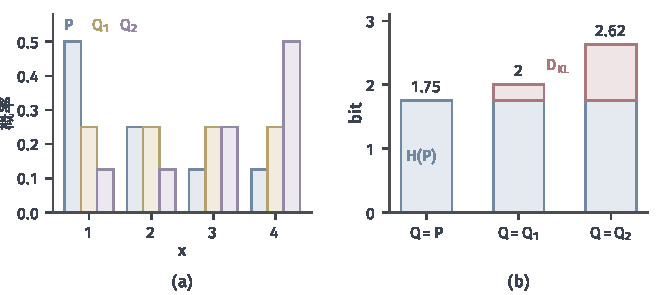
\includegraphics[width=112mm]{figures/07-probability/04-distribution-analysis/matplotlib/info-cross-entropy/figure.pdf}
  \caption{交叉熵的分解。(a)真实分布$P$（蓝）与两个参考分布$Q_1$（黄，均匀）、$Q_2$（紫）。(b)以bit计的$H(P,Q)$，蓝色部分是$H(P)=1.75$，红色部分是$D_{\mathrm{KL}}(P\Vert Q)$：$Q=P$时为$0$，$Q_1$时为$0.25$，$Q_2$时为$0.875$。}
  \label{fig:info-cross-entropy}
\end{BookInlineFigure}

图~\ref{fig:info-cross-entropy}显示，三种设计的蓝色部分一样高，差别全在红色部分。$Q_2$把最常见的结果当成最罕见的，失配最严重。

交叉熵的两个分布不能交换。真实分布为$Q_1$、参考分布为$P$时，四个字母等可能出现，而按$P$设计的题数是$1,2,3,3$，平均
\[
  H(Q_1,P)=\tfrac14(1+2+3+3)=2.25\neq H(P,Q_1)=2.
\]
两者的固有部分不同（$H(Q_1)=2$而$H(P)=1.75$），失配部分也不同（$0.25$与$0.25$恰好相等只是这个例子的巧合，一般不等）。若参考分布取$Q_3=(\tfrac12,\tfrac12,0,0)$，它完全没有为$c,d$留位置，$H(P,Q_3)=+\infty$。

\paragraph{熵为无穷时}
式~\eqref{eq:info-cross-entropy-decomposition}要求$H(P)<\infty$。若$H(P)=+\infty$，取$Q=P$，则$H(P,Q)=H(P)=+\infty$，而$D_{\mathrm{KL}}(P\Vert Q)=0$。这时“$D_{\mathrm{KL}}=H(P,Q)-H(P)$”是$\infty-\infty$，没有意义。KL散度直接由式~\eqref{eq:info-kl-recall}定义，不经过这个差。

\paragraph{连续情形}
对密度，交叉熵与微分熵一样依赖坐标。设$P=\mathcal{N}(0,1)$，$Q_s=\mathcal{N}(0,s^{2})$。参考分布分配的代价是
\[
  -\ln q_s(x)=\frac12\ln(2\pi s^{2})+\frac{x^{2}}{2s^{2}}.
\]
按$P$平均，用$\mathbb{E}_P[X^{2}]=1$，得到
\[
  H(P,Q_s)=\frac12\ln(2\pi s^{2})+\frac{1}{2s^{2}}.
\]
减去$h(P)=\tfrac12\ln(2\pi\mathrm{e})$，得到
\[
  D_{\mathrm{KL}}(P\Vert Q_s)=\ln s+\frac{1}{2s^{2}}-\frac12.
\]
$s=1$时为零；$s=2$时$H(P,Q_2)\approx1.737$，比$h(P)\approx1.419$多$0.318$。图~\ref{fig:info-gauss-cross}画出了整条曲线。

\begin{BookInlineFigure}
  \centering
  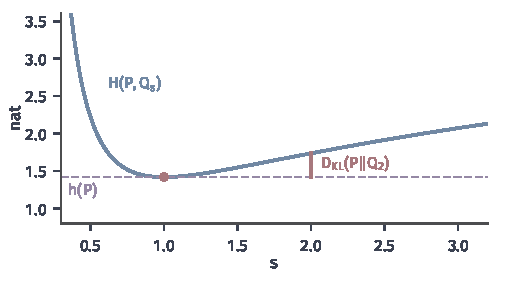
\includegraphics[width=86mm]{figures/07-probability/04-distribution-analysis/matplotlib/info-gauss-cross/figure.pdf}
  \caption{$P=\mathcal{N}(0,1)$相对于$Q_s=\mathcal{N}(0,s^{2})$的交叉熵（蓝），紫虚线为$h(P)\approx1.419$，单位nat。最小值在$s=1$（红点）处达到；红色竖线是$s=2$时的KL散度$0.318$。}
  \label{fig:info-gauss-cross}
\end{BookInlineFigure}

参考分布太窄（$s$小）时，交叉熵增长得很快：$P$的结果经常落在$Q_s$认为罕见的地方，每次都付很高的代价。太宽时增长较慢，只是对每个结果都略显“意外”。若把$x$换成$ax$，$h(P)$与$H(P,Q_s)$都增加$\ln\lvert a\rvert$，差$D_{\mathrm{KL}}$不变。连续情形下，有确定意义的是失配部分，而不是交叉熵本身的数值。

表~\ref{tab:info-entropy-cross}总结熵、交叉熵和KL散度的区别。

\begin{BookInlineTable}
  \centering
  \caption{熵、交叉熵与KL散度}
  \label{tab:info-entropy-cross}
  \begin{tabular}{@{}llll@{}}
    \toprule
    量 & 平均的对象 & 依赖坐标 & 下界\\
    \midrule
    $H(P)$或$h(P)$ & $P$下的$-\ln p$ & 连续时依赖 & 离散时$0$\\
    $H(P,Q)$ & $P$下的$-\ln q$ & 连续时依赖 & 离散时$H(P)$\\
    $D_{\mathrm{KL}}(P\Vert Q)$ & $P$下的$\ln(p/q)$ & 不依赖 & $0$\\
    \bottomrule
  \end{tabular}
\end{BookInlineTable}


\section{数据处理不等式}
\label{sec:info-data-processing}

观测$Y$含有关于$X$的信息$I(X;Y)$。实际中观测很少原样使用：读数会被四舍五入，记录会被压缩，信号会再经过一段有噪声的线路。处理后得到$Z$，它含有的关于$X$的信息能否比$Y$多？如果处理时只用了$Y$，没有再接触$X$的任何来源，答案应当是否定的。本节把“只用了$Y$”写成条件独立，再用互信息的链式法则证明这个直觉，并研究什么时候处理不损失信息。

\subsection{后处理的信息损失}
\label{sec:info-dpi-loss}

“$Z$只依赖$Y$”有两种说法。一种是生成方式：先有$(X,Y)$，再按一个只以$y$为输入的随机规则$K(y,\cdot)$产生$Z$，这个规则不看$X$。另一种是条件独立：$X\perp\!\!\!\perp Z\mid Y$。第~\ref{chap:conditional-distributions}章证明了两种说法在标准Borel空间上等价。满足这个条件时，称$X,Y,Z$构成\term{Markov链}（Markov chain），记作$X\to Y\to Z$。确定性处理$Z=g(Y)$是特例，规则$K(y,\cdot)$是点质量。

\begin{theorem}[数据处理不等式]
\label{thm:info-data-processing}
设$X,Y,Z$取值于标准Borel空间，$X\to Y\to Z$。则
\begin{equation}
  I(X;Z)\leq I(X;Y).
  \label{eq:info-data-processing}
\end{equation}
\end{theorem}

\begin{proof}
用链式法则~\eqref{eq:info-mi-chain-rule}按两种顺序展开$I(X;Y,Z)$。先$Y$后$Z$：
\[
  I(X;Y,Z)=I(X;Y)+I(X;Z\mid Y)=I(X;Y),
\]
其中$I(X;Z\mid Y)=0$由条件独立与定理~\ref{thm:info-conditional-mi-zero}得到。先$Z$后$Y$：
\[
  I(X;Y,Z)=I(X;Z)+I(X;Y\mid Z)\geq I(X;Z),
\]
因为条件互信息非负。两式合并即得式~\eqref{eq:info-data-processing}。整个论证只是非负量的相加和比较，在$[0,+\infty]$中进行，不需要任何熵有限。
\end{proof}

式~\eqref{eq:info-data-processing}称为\term{数据处理不等式}（data processing inequality）。证明还给出了损失的大小。若$I(X;Y)<\infty$，两种展开相等，移项得到
\begin{equation}
  I(X;Y)-I(X;Z)=I(X;Y\mid Z).
  \label{eq:info-dpi-gap}
\end{equation}
处理损失的信息，正是已知$Z$以后$Y$还能提供的关于$X$的信息。

\paragraph{两个例子}
图~\ref{fig:info-markov-chain}(a)是确定性的合并。$X$在$\{0,1,2,3\}$上均匀，$Y=X$，$Z=\lfloor Y/2\rfloor$把$0,1$并成$0$，把$2,3$并成$1$。由定理~\ref{thm:info-mi-entropy}，
\[
  I(X;Y)=H(X)=\ln4,\qquad I(X;Z)=H(Z)=\ln2.
\]
合并丢掉了“在组内是哪一个”这一位信息，损失$I(X;Y\mid Z)=\ln2$。

\begin{BookInlineFigure}
  \centering
  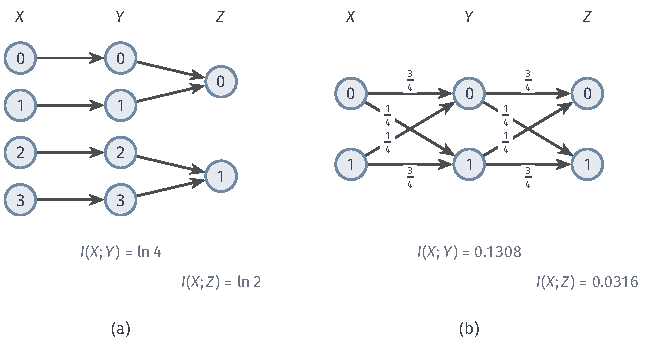
\includegraphics[width=110.1mm]{figures/07-probability/04-distribution-analysis/tikz/info-markov-chain/figure.pdf}
  \caption{两条Markov链$X\to Y\to Z$，箭头为转移概率。(a)$X$在四个标签上均匀，$Y=X$，$Z=\lfloor Y/2\rfloor$合并相邻标签。(b)公平硬币$X$经两段独立的线路，每段以概率$\tfrac14$翻转。下方为与$X$的互信息（nat）。}
  \label{fig:info-markov-chain}
\end{BookInlineFigure}

图~\ref{fig:info-markov-chain}(b)是添加独立噪声。$Y$是$X$经以概率$\tfrac14$出错的线路得到的，$Z$是$Y$再经一段独立的、以概率$\varepsilon_2$出错的线路得到的。$Z\neq X$当且仅当恰好一段出错，所以$X$到$Z$的总出错概率是
\[
  \tfrac14(1-\varepsilon_2)+\tfrac34\varepsilon_2.
\]
$\varepsilon_2=\tfrac14$时为$\tfrac38$，于是
\[
  I(X;Z)=\ln2-h_{\mathrm{b}}(\tfrac38)\approx0.0316<I(X;Y)\approx0.1308.
\]
图~\ref{fig:info-dpi-cascade}画出$I(X;Z)$随$\varepsilon_2$的变化：第二段线路越不可靠，剩下的信息越少，$\varepsilon_2=\tfrac12$时降为零。无论第二段怎样设计，曲线都不会越过$I(X;Y)$。

\begin{BookInlineFigure}
  \centering
  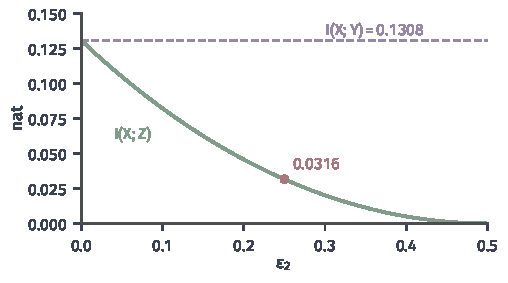
\includegraphics[width=86mm]{figures/07-probability/04-distribution-analysis/matplotlib/info-dpi-cascade/figure.pdf}
  \caption{两段串联线路。第一段翻转概率$\tfrac14$，第二段为$\varepsilon_2$。绿线为$I(X;Z)$，紫虚线为$I(X;Y)\approx0.1308$，单位nat；红点为$\varepsilon_2=\tfrac14$时的$0.0316$。}
  \label{fig:info-dpi-cascade}
\end{BookInlineFigure}

\paragraph{两个推论}
取$Z=g(Y)$为任意可测函数，得到$I(X;g(Y))\leq I(X;Y)$：任何对观测的计算都不能增加关于$X$的信息。再取离散的$X$并令$Y=X$，联合质量$p_{X,g(X)}(x,g(x))=p_X(x)$，代入式~\eqref{eq:info-mutual-information-discrete}，比值是$1/p_{g(X)}(g(x))$，所以$I(X;g(X))=H(g(X))$，特别地$I(X;X)=H(X)$。于是
\[
  H(g(X))\leq H(X).
\]
对离散变量作函数变换只会合并取值，熵不增；$g$是单射时取等号。注意微分熵没有这个性质，式~\eqref{eq:info-differential-entropy-scale}中$\lvert a\rvert>1$时$h(aX)>h(X)$。

\paragraph{条件独立的作用}
定理的前提不能去掉。仍看图~\ref{fig:info-markov-chain}(b)的第一段：$Y=X\oplus N$，$N$是翻转噪声。若处理者碰巧知道$N$，令$Z=Y\oplus N$，则$Z=X$，$I(X;Z)=\ln2$，远大于$I(X;Y)$。这里$Z$不只依赖$Y$，还依赖与$X$在给定$Y$时相关的$N$：给定$Y=y$时，$N=0$当且仅当$X=y$。所以$X\perp\!\!\!\perp Z\mid Y$不成立。“只用了$Y$”的确切意思是：处理中引入的额外随机性，在给定$Y$时与$X$独立。

条件独立是对称的：$X\perp\!\!\!\perp Z\mid Y$等价于$Z\perp\!\!\!\perp X\mid Y$，所以$X\to Y\to Z$也是$Z\to Y\to X$，同样有$I(X;Z)\leq I(Y;Z)$。箭头只是书写习惯。Markov链描述的是联合分布的一种结构，信息在其中两端都要经过$Y$；它并不规定哪个变量产生了哪个变量。同一个联合分布既可以由“$X$经过线路得到$Y$”产生，也可以由“先抽$Y$、再按后验抽$X$”产生，不等式对两者相同。

\subsection{信息保留}
\label{sec:info-dpi-preservation}

数据处理不等式什么时候取等号？最简单的情形是处理可以撤销。设$Z=g(Y)$，其中$g$是可测双射，逆映射也可测。则$X\to Y\to Z$，同时$Y=g^{-1}(Z)$，又有$X\to Z\to Y$。对两条链分别应用定理~\ref{thm:info-data-processing}，得到
\[
  I(X;Z)\leq I(X;Y)\leq I(X;Z),
\]
所以$I(X;g(Y))=I(X;Y)$。对两个变量分别作这样的变换，互信息都不变；这与微分熵随坐标改变形成对比。

可逆是充分条件，不是必要条件。设$X$是公平硬币，$U$是与$X$独立的公平硬币，观测$Y=2X+U\in\{0,1,2,3\}$，处理为$Z=\lfloor Y/2\rfloor$。$Z=X$，所以
\[
  I(X;Z)=H(X)=\ln2.
\]
另一方面，$X$是$Y$的函数，$I(X;Y)=H(X)-H(X\mid Y)=\ln2$。处理把四个值并成两个，不可逆，却没有损失任何关于$X$的信息：被丢掉的$U$与$X$无关。

一般的判据由式~\eqref{eq:info-dpi-gap}给出。

\begin{theorem}[信息保留的条件]
\label{thm:info-dpi-equality}
设$X,Y,Z$取值于标准Borel空间，$X\to Y\to Z$，并且$I(X;Y)<\infty$。则$I(X;Z)=I(X;Y)$当且仅当$X\perp\!\!\!\perp Y\mid Z$，即$X\to Z\to Y$也成立。
\end{theorem}

\begin{proof}
由式~\eqref{eq:info-dpi-gap}，等号当且仅当$I(X;Y\mid Z)=0$，再由定理~\ref{thm:info-conditional-mi-zero}，这等价于$X\perp\!\!\!\perp Y\mid Z$。
\end{proof}

$X\to Z\to Y$说的是：知道$Z$以后，$Y$中剩下的部分与$X$无关。上面的例子中，给定$Z=X$以后，$Y$只多出一个独立的$U$，确实与$X$条件独立。在图~\ref{fig:info-markov-chain}(a)中，给定$Z=0$时$Y$在$\{0,1\}$中仍随$X$变化，条件独立不成立，信息有损失。

定理要求$I(X;Y)<\infty$，因为式~\eqref{eq:info-dpi-gap}要移项。互信息为无穷时，$I(X;Z)=I(X;Y)=\infty$可以与“有损失”同时出现。设$X\sim\operatorname{Unif}(0,1)$，$Y=X$，$Z$由$X$二进制展开的奇数位组成。$Z$本身服从无原子的分布，并且是$X$的函数，与第~\ref{sec:info-mi-definition}节的对角线论证相同，联合分布集中在一个函数图像上，而边缘乘积给这个图像零概率，所以$I(X;Z)=+\infty=I(X;Y)$。但给定$Z$以后，$X$的偶数位仍是独立均匀的，$Y=X$与$X$之间还有无穷多的信息，$I(X;Y\mid Z)=+\infty$。两边都是无穷，比较互信息的数值已经看不出损失，要直接看条件互信息。


\section{辨别错误的下界}
\label{sec:info-fano}

一个标签$X$取$M$个值之一，我们只能看到与它相关的观测$Y$，要根据$Y$猜出$X$。无论怎样设计判别规则，错误概率能否降到任意小？直觉上，若看到$Y$以后$X$仍然很不确定，就不可能总猜对。本节把这个直觉定量化：剩余的不确定性$H(X\mid Y)$给错误概率一个下界。随后把它改写为互信息的形式，这是证明“信息不够时无法可靠辨别”的通用工具。

\subsection{Fano不等式}
\label{sec:info-fano-inequality}

先固定设定。$X$取值于$M\geq2$个元素的有限集合$\mathcal{X}$；观测$Y$取值于标准Borel空间，可以是离散的，也可以是连续的。判别规则是可测函数$g$，猜测$\hat{X}=g(Y)\in\mathcal{X}$，错误概率$P_{\mathrm{e}}=\mathbb{P}(\hat{X}\neq X)$。

$Y$不一定离散，所以条件熵按正则条件分布逐个$y$定义：
\[
  H(X\mid Y)=\int H\bigl(P_{X\mid Y}(\cdot\mid y)\bigr)\,P_Y(\mathrm{d}y),
\]
其中$H(\cdot)$是有限概率表的熵。$Y$离散时它就是式~\eqref{eq:info-conditional-entropy}。

\begin{theorem}[Fano不等式]
\label{thm:info-fano}
在上述设定下，
\begin{equation}
  H(X\mid Y)\leq h_{\mathrm{b}}(P_{\mathrm{e}})+P_{\mathrm{e}}\ln(M-1).
  \label{eq:info-fano}
\end{equation}
\end{theorem}

式~\eqref{eq:info-fano}称为\term{Fano不等式}（Fano's inequality）。证明的想法是引入错误指示$E=\mathbf{1}_{\{\hat{X}\neq X\}}$，把“确定$X$”拆成两步：先确定是否猜错，再在猜错时确定$X$是其余$M-1$个值中的哪一个。第一步最多需要$h_{\mathrm{b}}(P_{\mathrm{e}})$，第二步只在猜错时才需要，最多$\ln(M-1)$。

\begin{proof}
固定$y$，在条件分布$P_{X\mid Y}(\cdot\mid y)$下考虑离散变量$X$与$E=\mathbf{1}_{\{g(y)\neq X\}}$。$E$是$X$的函数，所以$(X,E)$与$X$的概率表只差零概率的格，二者熵相等。对$(E,X)$用链式法则，先揭示$E$：
\[
  H(X\mid Y=y)=H(E\mid Y=y)+H(X\mid E,Y=y).
\]
记$e(y)=\mathbb{P}(X\neq g(y)\mid Y=y)$。第一项是$h_{\mathrm{b}}(e(y))$。第二项中，$E=0$时$X=g(y)$已确定，熵为$0$；$E=1$时$X$在$\mathcal{X}\setminus\{g(y)\}$的$M-1$个值中，由定理~\ref{thm:info-entropy-range}熵至多$\ln(M-1)$。所以
\[
  H(X\mid Y=y)\leq h_{\mathrm{b}}(e(y))+e(y)\ln(M-1).
\]
对$P_Y$积分，$\int e(y)\,P_Y(\mathrm{d}y)=P_{\mathrm{e}}$。$h_{\mathrm{b}}$凹，由Jensen不等式，
\[
  \int h_{\mathrm{b}}(e(y))\,P_Y(\mathrm{d}y)\leq h_{\mathrm{b}}(P_{\mathrm{e}}).
\]
两部分合起来即得式~\eqref{eq:info-fano}。
\end{proof}

若判别时还使用了与$(X,Y)$独立的随机数$U$，把$(Y,U)$看成观测即可：$U$与$(X,Y)$独立，所以给定$(Y,U)$时$X$的条件分布与给定$Y$时相同，$H(X\mid Y,U)=H(X\mid Y)$，定理不变。

\paragraph{怎样读这个不等式}
记右端为$\phi_M(p)=h_{\mathrm{b}}(p)+p\ln(M-1)$。求导得$\phi_M'(p)=\ln\frac{(1-p)(M-1)}{p}$，在$p<(M-1)/M$时为正，所以$\phi_M$在$[0,(M-1)/M]$上严格递增，从$0$升到$\phi_M((M-1)/M)=\ln M$。于是，若$H(X\mid Y)=c>0$，任何规则的错误概率都不小于方程$\phi_M(p)=c$在这段区间上的解。剩余不确定性越大，错误下界越高；$H(X\mid Y)=0$时下界为零，与$X$可由$Y$确定一致。

由$h_{\mathrm{b}}(p)\leq\ln2$，可以得到一个便于计算的较弱形式：$M\geq3$时，
\begin{equation}
  P_{\mathrm{e}}\geq\frac{H(X\mid Y)-\ln2}{\ln(M-1)}.
  \label{eq:info-fano-weak}
\end{equation}
它在$H(X\mid Y)\leq\ln2$时没有用处，在标签很多时与精确形式相差不大。

\paragraph{等号可以达到}
设$M=4$，$X$在$\{1,2,3,4\}$上均匀；观测$Y$以概率$0.7$等于$X$，以概率$0.1$等于其余三个值中的每一个。由对称性，给定$Y=y$时，$X=y$的后验概率是$0.7$，其余三个值各$0.1$。于是
\[
  H(X\mid Y)=H(0.7,0.1,0.1,0.1)=h_{\mathrm{b}}(0.3)+0.3\ln3\approx0.940\ \mathrm{nat}.
\]
猜$\hat{X}=Y$的错误概率是$0.3$，代入式~\eqref{eq:info-fano}右端恰好也是$0.940$：等号成立。由$\phi_4$的单调性，任何规则的错误概率都至少是$0.3$，所以猜$\hat{X}=Y$已是最好的规则。

\begin{BookInlineFigure}
  \centering
  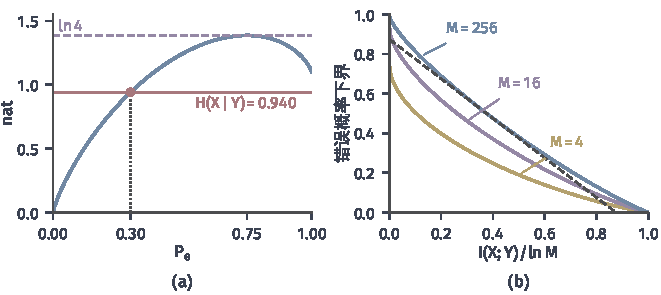
\includegraphics[width=112mm]{figures/07-probability/04-distribution-analysis/matplotlib/info-fano/figure.pdf}
  \caption{Fano不等式。(a)$M=4$时$\phi_4(P_{\mathrm{e}})=h_{\mathrm{b}}(P_{\mathrm{e}})+P_{\mathrm{e}}\ln3$（蓝），在$P_{\mathrm{e}}=\tfrac34$处达到$\ln4$（紫虚线）。红线为四值对称观测例子的$H(X\mid Y)\approx0.940$，与曲线交于$P_{\mathrm{e}}=0.3$。(b)$X$均匀时Fano给出的最小错误概率，横轴为$I(X;Y)/\ln M$，$M=4,16,256$；灰虚线为$M=256$时式~\eqref{eq:info-fano-mi}的较弱形式。}
  \label{fig:info-fano}
\end{BookInlineFigure}

等号成立的条件从证明中可以读出：每个$y$下错误概率相同（Jensen取等），并且猜错时其余$M-1$个值等可能。上面的例子两条都满足。一般情形下Fano不等式只是下界，实际最小错误可以大得多。

定理只适用于有限个标签和“猜错与否”这种错误标准。若要估计的是连续参数，“猜中”的概率通常为零，不等式不能直接使用；需要先从参数中挑出有限个相互分开的候选，把估计问题改写成在它们之间辨别，下一小节会看到这种改写的样子。

\subsection{通信与统计辨别}
\label{sec:info-fano-applications}

当$X$在$M$个标签上均匀时，$H(X)=\ln M$，由式~\eqref{eq:info-mi-entropy-difference}，$H(X\mid Y)=\ln M-I(X;Y)$。这里$Y$可以不是离散的，第~\ref{sec:info-mi-entropy}节的证明逐个条件值进行，同样成立。代入较弱形式（这次用$\ln M$代替$\ln(M-1)$，对$M=2$也适用），得到
\begin{equation}
  P_{\mathrm{e}}\geq1-\frac{I(X;Y)+\ln2}{\ln M}.
  \label{eq:info-fano-mi}
\end{equation}
这个形式只需要互信息：要以小错误区分$M$个等可能的标签，观测至少要提供约$\ln M$的信息。四值对称观测的例子中$I(X;Y)=\ln4-0.940\approx0.446$，式~\eqref{eq:info-fano-mi}给出$P_{\mathrm{e}}\geq0.178$，比精确形式的$0.3$弱。图~\ref{fig:info-fano}(b)比较了不同$M$时的精确下界：横轴按$\ln M$归一化后，$M$越大，曲线越接近直线$1-I/\ln M$。

\paragraph{通信}
在有噪声的线路上传送消息时，消息$W$从$M$个中均匀选出，编码成线路输入$X_1,\dots,X_n$，线路输出$Y_1,\dots,Y_n$，接收方据此猜出$\hat{W}$。码率$R=\ln M/n$是每次使用线路平均传送的信息。由于$\hat{W}$只依赖输出，$W\to(Y_1,\dots,Y_n)\to\hat{W}$；由于输出只经由输入依赖消息，数据处理不等式给出
\[
  I(W;Y_1,\dots,Y_n)\leq I(X_1,\dots,X_n;Y_1,\dots,Y_n).
\]
第~\ref{chap:discrete-channel-capacity}章会证明，对每次使用相互独立的线路，右端不超过$nC$，$C$是单次使用的容量。代入式~\eqref{eq:info-fano-mi}，得到
\[
  P_{\mathrm{e}}\geq1-\frac{nC+\ln2}{nR}=1-\frac{C}{R}-\frac{\ln2}{nR}.
\]
若$R>C$，$n\to\infty$时右端趋于$1-C/R>0$，错误概率不能趋于零。这里的错误概率是按均匀消息平均的；逐个消息的最大错误概率不小于平均值，下界对它同样成立。

\paragraph{统计辨别}
设有$M$个候选分布$P_1,\dots,P_M$，标签$J$均匀选出，观测是来自$P_J$的独立同分布样本$X_1,\dots,X_n$，要从样本猜出$J$。这时需要的是$I(J;X_1,\dots,X_n)$的上界。

离散情形下，对任意分布$Q$，记$\bar{P}=\tfrac1M\sum_jP_j$为观测的边缘分布，在各项有限时直接展开对数可以核对
\[
  \frac1M\sum_{j=1}^{M}D_{\mathrm{KL}}(P_j\Vert Q)=I(J;X)+D_{\mathrm{KL}}(\bar{P}\Vert Q),
\]
依据是对数比的拆分
\[
  \ln\frac{p_j(x)}{q(x)}=\ln\frac{p_j(x)}{\bar{p}(x)}+\ln\frac{\bar{p}(x)}{q(x)}.
\]
按权重$\tfrac1Mp_j(x)$对$j$与$x$求和，第一项给出$I(J;X)$（$(J,X)$的联合质量是$\tfrac1Mp_j(x)$，边缘乘积是$\tfrac1M\bar{p}(x)$），第二项给出$D_{\mathrm{KL}}(\bar{P}\Vert Q)$。右端第二项非负，所以
\[
  I(J;X)\leq\frac1M\sum_{j=1}^{M}D_{\mathrm{KL}}(P_j\Vert Q).
\]
取$Q$为某个候选$P_k$，就得到$I(J;X)\leq\max_{j,k}D_{\mathrm{KL}}(P_j\Vert P_k)$。$n$个独立样本时，乘积分布的对数比是各样本对数比之和，KL随之乘以$n$。于是
\[
  P_{\mathrm{e}}\geq1-\frac{n\max_{j,k}D_{\mathrm{KL}}(P_j\Vert P_k)+\ln2}{\ln M}.
\]

例如$M=8$个候选$\mathcal{N}(\theta_j,1)$，$\theta_j=0,0.1,\dots,0.7$。按定义计算，
\[
  D_{\mathrm{KL}}\bigl(\mathcal{N}(a,1)\Vert\mathcal{N}(b,1)\bigr)=\mathbb{E}\Bigl[\frac{(X-b)^{2}-(X-a)^{2}}{2}\Bigr]=\frac{(a-b)^{2}}{2},
\]
期望对$X\sim\mathcal{N}(a,1)$取。最大值是$0.7^{2}/2=0.245$，一个样本时$P_{\mathrm{e}}\geq1-(0.245+\ln2)/\ln8\approx0.549$。候选越密、样本越少，辨别越难；要让下界失效，样本数须与$\ln M/\max D_{\mathrm{KL}}$同阶。

这两个应用用的是同一个工具，但要分别核对三件事：标签是否均匀（Fano给的是平均错误）、观测是怎样由标签产生的（决定互信息的上界）、错误按什么标准计算。把估计连续参数的误差转成在候选之间的辨别错误，是卷八的工作，可参考\BookChapterRef{chap:finite-sample-lower-bounds}{卷八第5章“有限样本的精度下界”}。


\section{互信息的辨别下界}
\label{sec:info-infonce}

上一节用互信息的上界推出辨别错误的下界。这一节方向相反：互信息本身难以计算时，用一个辨别问题做得有多好，给出互信息的下界。

互信息需要联合分布与边缘乘积的密度比$r=\mathrm{d}P_{X,Y}/\mathrm{d}(P_X\otimes P_Y)$，再对它取对数积分。在高维连续空间里，$r$常常写不出来，积分也难以计算；但从$P_{X,Y}$抽取配对$(X,Y)$、从$P_Y$抽取单个$Y$往往很容易。于是考虑一个辅助问题：把一个真正与$X$配对的$Y$藏在一堆与$X$无关的候选中，让一个评分规则把它找出来。$X$与$Y$关联越强，真配对越容易被认出；找得好，就说明互信息至少有这么大。

\subsection{候选配对的构造}
\label{sec:info-infonce-construction}

设$X,Y$取值于标准Borel空间，联合分布$P_{X,Y}$，正则条件分布$P_{Y\mid X}$存在。固定候选数$N\geq2$，按下面的方式产生$(X,J,Y_1,\dots,Y_N)$：
\begin{enumerate}
  \item 抽取$X\sim P_X$，并独立地从$\{1,\dots,N\}$中均匀抽取隐藏位置$J$；
  \item 给定$X=x$、$J=j$，令$Y_j\sim P_{Y\mid X}(\cdot\mid x)$，其余$Y_k\sim P_Y$（$k\neq j$），这$N$个候选在给定$(X,J)$时相互独立。
\end{enumerate}
记观测为$W=(X,Y_1,\dots,Y_N)$，$J$不被观测。图~\ref{fig:info-infonce-construction}画出了$N=4$时的构造。

\begin{BookInlineFigure}
  \centering
  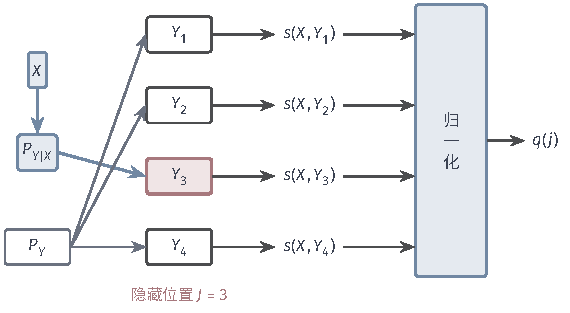
\includegraphics[width=96.4mm]{figures/07-probability/04-distribution-analysis/tikz/info-infonce-construction/figure.pdf}
  \caption{$N=4$个候选的构造。隐藏位置$J=3$（红框）的候选按给定$X$的条件分布$P_{Y\mid X}$产生（蓝），其余候选独立地按边缘分布$P_Y$产生（灰）。评分$s(X,Y_j)$经指数归一化得到对隐藏位置的猜测$q(j)$。}
  \label{fig:info-infonce-construction}
\end{BookInlineFigure}

这个构造有三条基本性质，后面的证明都靠它们。

\begin{lemma}[候选的分布]
\label{lem:info-infonce-structure}
在上述构造中：
\begin{enumerate}
  \item $J$与$X$独立；
  \item $(Y_1,\dots,Y_N)$独立同分布于$P_Y$，并且与$J$独立；
  \item 给定$J=j$，$(X,Y_j)$的分布是$P_{X,Y}$，其余候选独立同分布于$P_Y$，并与$(X,Y_j)$独立。
\end{enumerate}
\end{lemma}

\begin{proof}
第一条是构造的第一步。第三条：给定$J=j$，$X\sim P_X$且$Y_j$按$P_{Y\mid X}$产生，所以$(X,Y_j)\sim P_{X,Y}$；其余候选的条件分布不依赖$X$，所以与$(X,Y_j)$独立。第二条：在第三条中对$X$积分，$Y_j$的分布是$P_Y$，其余候选也是$P_Y$，且相互独立；这个分布不依赖$j$，所以候选组与$J$独立。
\end{proof}

第二条说明，单看候选组而不看$X$，完全看不出哪个是真配对；隐藏位置的线索只能来自$X$与各候选之间的关联。

\paragraph{隐藏位置的后验}
设$P_{X,Y}\ll P_X\otimes P_Y$，密度比为$r(x,y)$；$I(X;Y)<\infty$时这总成立。由引理~\ref{lem:info-infonce-structure}第三条，给定$J=j$时$W$的分布是$P_{X,Y_j}\otimes P_Y^{\otimes(N-1)}$，它相对于参考分布$P_X\otimes P_Y^{\otimes N}$的密度是$r(x,y_j)$。$J$的先验是$1/N$，由Bayes公式，
\begin{equation}
  \mathbb{P}(J=j\mid W)=\frac{r(X,Y_j)}{\sum_{k=1}^{N}r(X,Y_k)},\qquad j=1,\dots,N.
  \label{eq:info-infonce-posterior}
\end{equation}
分母几乎必然为正，因为真配对一项$r(X,Y_J)$几乎必然为正。后验只依赖各候选的密度比：与$X$越“般配”的候选，越可能是真配对。$X$与$Y$独立时$r\equiv1$，后验是均匀分布，候选无从区分。

\paragraph{二元例子}
仍用公平硬币$X$经以概率$\tfrac14$出错的线路得到$Y$。密度比在$y=x$时为$\tfrac{3/8}{1/4}=\tfrac32$，在$y\neq x$时为$\tfrac12$。取$N=2$。若两个候选相同（都等于$X$或都不等于$X$），后验是$(\tfrac12,\tfrac12)$；若只有一个等于$X$，由式~\eqref{eq:info-infonce-posterior}，它是真配对的后验概率为
\[
  \frac{3/2}{3/2+1/2}=\frac34.
\]
真配对等于$X$的概率是$\tfrac34$，另一个候选与$X$无关、是公平硬币，所以两个候选不同的概率恰为$\tfrac12$。

\subsection{InfoNCE下界}
\label{sec:info-infonce-bound}

实际中密度比$r$未知，用一个可测的实值\term{配对评分}（critic）函数$s(x,y)$代替$\ln r$，把评分作指数归一化得到对隐藏位置的猜测：
\begin{equation}
  q_s(j\mid W)=\frac{\mathrm{e}^{s(X,Y_j)}}{\sum_{k=1}^{N}\mathrm{e}^{s(X,Y_k)}}.
  \label{eq:info-infonce-softmax}
\end{equation}
用真实位置的平均负对数概率衡量猜得好坏，
\begin{equation}
  L(s)=\mathbb{E}\bigl[-\ln q_s(J\mid W)\bigr]\in[0,+\infty].
  \label{eq:info-infonce-loss}
\end{equation}
$L(s)$是真实后验相对于猜测$q_s$的交叉熵按$W$的平均。以$L$为目标的方法通称InfoNCE（信息噪声对比估计），它的总体值给出互信息的下界。

\begin{theorem}[InfoNCE下界]
\label{thm:info-infonce}
设$X,Y$取值于标准Borel空间，$I(X;Y)<\infty$，$N\geq2$，$s$是任意可测实值评分函数。则
\begin{equation}
  \ln N-L(s)\leq I(X;Y).
  \label{eq:info-infonce-bound}
\end{equation}
更精确地，
\begin{equation}
  I(X;Y)-\bigl(\ln N-L(s)\bigr)=I(X;Y_1,\dots,Y_N)+\mathbb{E}\Bigl[D_{\mathrm{KL}}\bigl(P_{J\mid W}\Vert q_s(\cdot\mid W)\bigr)\Bigr].
  \label{eq:info-infonce-gap}
\end{equation}
\end{theorem}

证明分三步：猜测的交叉熵不小于后验的熵；后验的熵等于$\ln N$减去隐藏位置与观测的互信息；这个互信息不超过原配对的互信息。

\begin{proof}
\emph{第一步。}固定$W=w$，$J$的后验$\pi(\cdot\mid w)$是$N$个点上的概率表。由定理~\ref{thm:info-cross-entropy-decomposition}（$N$点上的熵有限），
\[
  \mathbb{E}\bigl[-\ln q_s(J\mid W)\bigm|W=w\bigr]=H\bigl(\pi(\cdot\mid w)\bigr)+D_{\mathrm{KL}}\bigl(\pi(\cdot\mid w)\Vert q_s(\cdot\mid w)\bigr).
\]
对$W$平均，左端是$L(s)$，右端第一项是$H(J\mid W)$，于是
\[
  L(s)=H(J\mid W)+\mathbb{E}\bigl[D_{\mathrm{KL}}(P_{J\mid W}\Vert q_s(\cdot\mid W))\bigr]\geq H(J\mid W).
\]

\emph{第二步。}$J$均匀，$H(J)=\ln N$有限，由式~\eqref{eq:info-mi-entropy-difference}（对一般的$W$逐条件值进行），
\[
  H(J\mid W)=\ln N-I(J;W).
\]

\emph{第三步。}记$\bm{Y}=(Y_1,\dots,Y_N)$。用链式法则~\eqref{eq:info-mi-chain-rule}展开$I(J;W)=I(J;\bm{Y},X)$，由引理第二条$I(J;\bm{Y})=0$，所以
\[
  I(J;W)=I(J;X\mid\bm{Y}).
\]
另一方面，用两种顺序展开$I(X;J,\bm{Y})$。先$J$后$\bm{Y}$：由引理第一条$I(X;J)=0$；由引理第三条，给定$J=j$时只有$Y_j$与$X$相关，再用一次链式法则得$I(X;\bm{Y}\mid J)=I(X;Y)$。于是
\[
  I(X;J,\bm{Y})=I(X;Y).
\]
先$\bm{Y}$后$J$：
\[
  I(X;J,\bm{Y})=I(X;\bm{Y})+I(X;J\mid\bm{Y}).
\]
两式相等，而$I(X;Y)<\infty$，所以各项有限，可以移项，并由条件互信息的对称性得到
\[
  I(J;W)=I(X;J\mid\bm{Y})=I(X;Y)-I(X;\bm{Y}).
\]

三步合起来，
\[
  \ln N-L(s)=I(X;Y)-I(X;\bm{Y})-\mathbb{E}\bigl[D_{\mathrm{KL}}(P_{J\mid W}\Vert q_s)\bigr].
\]
这就是式~\eqref{eq:info-infonce-gap}；右端两个减项都非负，得到式~\eqref{eq:info-infonce-bound}。若$L(s)=+\infty$，式~\eqref{eq:info-infonce-bound}左端为$-\infty$，自然成立。
\end{proof}

式~\eqref{eq:info-infonce-gap}说明下界与真值之间有两段差距。第二段来自评分函数：只有$q_s$等于真实后验时才消失，由式~\eqref{eq:info-infonce-posterior}，这要求$s(x,y)=\ln r(x,y)+c(x)$，其中$c(x)$只依赖$x$（它在归一化中相消）。第一段$I(X;\bm{Y})$与评分无关，是辅助问题本身的损失：$X$与整组候选的互信息。它非负，所以即使评分最优，下界一般也严格小于$I(X;Y)$。

\paragraph{二元例子的计算}
取最优评分$s=\ln r$。$N=2$时，上一小节已得到：以概率$\tfrac12$两个候选相同，后验熵为$\ln2$；以概率$\tfrac12$两者不同，后验为$(\tfrac34,\tfrac14)$，熵为$h_{\mathrm{b}}(\tfrac14)$。于是
\[
  H(J\mid W)=\tfrac12\ln2+\tfrac12h_{\mathrm{b}}(\tfrac14)\approx0.3466+0.2812=0.6277.
\]
下界为
\[
  \ln2-L(\ln r)=\ln2-H(J\mid W)\approx0.0654,
\]
恰为$I(X;Y)\approx0.1308$的一半；由式~\eqref{eq:info-infonce-gap}，另一半是$I(X;\bm{Y})$。候选数增加时，计算方法相同：给定$X$，真配对以概率$\tfrac34$与$X$相同，其余$N-1$个候选各以概率$\tfrac12$与$X$相同，按相同候选的个数$m$求和，后验在相同者上为$\tfrac{3/2}{Z}$、在其余者上为$\tfrac{1/2}{Z}$，$Z=\tfrac32m+\tfrac12(N-m)$。

\begin{BookInlineFigure}
  \centering
  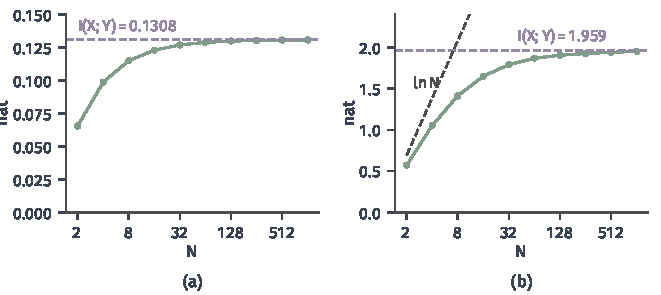
\includegraphics[width=112mm]{figures/07-probability/04-distribution-analysis/matplotlib/info-infonce-bound/figure.pdf}
  \caption{最优评分下的InfoNCE下界$\ln N-L$（绿）随候选数$N$的变化，横轴为对数刻度，紫虚线为$I(X;Y)$。(a)二元例子，按相同候选个数精确求和：$N=2,4,16,1024$时为$0.0654,0.0987,0.1229,0.1307$。(b)相关系数$0.99$的二元标准正态，$I(X;Y)\approx1.959$；Monte Carlo估计，种子$0$，每个$N$用$40000$组样本，标准误不超过$0.005$；灰虚线为$\ln N$。}
  \label{fig:info-infonce-bound}
\end{BookInlineFigure}

图~\ref{fig:info-infonce-bound}(a)中，下界随$N$增加逐渐逼近$I(X;Y)$：候选越多，$X$与整组候选的互信息在总量中所占的份额越小。这与“多个干扰项中认出真配对”的直觉一致，干扰项越多，认出真配对越能说明关联强。

\subsection{下界的限制}
\label{sec:info-infonce-limits}

\paragraph{候选数的上限}
$q_s\leq1$，所以$L(s)\geq0$，从而
\[
  \ln N-L(s)\leq\ln N.
\]
无论评分多好，下界都不超过$\ln N$。$I(X;Y)$很大时，要让下界接近它，候选数须达到$\mathrm{e}^{I(X;Y)}$的量级。图~\ref{fig:info-infonce-bound}(b)中相关系数为$0.99$的正态配对，$I(X;Y)\approx1.959$，$\mathrm{e}^{1.959}\approx7.1$；$N=2$时下界只有$0.57$，比$\ln2$略小，$N=8$时约$1.41$，直到$N$达到数百才接近真值。互信息每增加$1$ nat，所需候选数约乘以$\mathrm{e}$。

\paragraph{评分函数的限制}
评分函数通常只能从一个给定的函数类中选。在二元例子中限定$s(x,y)=c\,\mathbf{1}_{\{x=y\}}$，只调一个参数$c$。$N=2$时可以逐项算出$\ln2-L$：两个候选相同时$q$均匀；不同时真配对与$X$相同的概率是$\tfrac34$，被赋予$\mathrm{e}^{c}/(\mathrm{e}^{c}+1)$。于是
\[
  L(c)=\tfrac12\ln2+\tfrac12\Bigl[\tfrac34\ln(1+\mathrm{e}^{-c})+\tfrac14\ln(1+\mathrm{e}^{c})\Bigr].
\]
令导数为零得$\mathrm{e}^{c}=3$，$c=\ln3$正是$\ln\tfrac32-\ln\tfrac12$，这时评分等于$\ln r$加常数，下界达到$0.0654$。

\begin{BookInlineFigure}
  \centering
  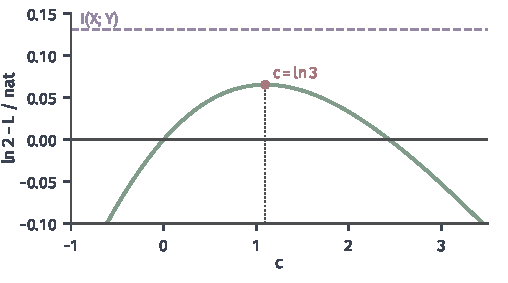
\includegraphics[width=86mm]{figures/07-probability/04-distribution-analysis/matplotlib/info-infonce-score/figure.pdf}
  \caption{二元例子、$N=2$、评分限定为$s(x,y)=c\,\mathbf{1}_{\{x=y\}}$时的$\ln2-L$（绿），紫虚线为$I(X;Y)\approx0.1308$。最大值在$c=\ln3$（红点）处，为$0.0654$；$c=0$时为$0$，$c=3$时约为$-0.053$。}
  \label{fig:info-infonce-score}
\end{BookInlineFigure}

图~\ref{fig:info-infonce-score}显示，$c=0$时评分不区分候选，下界为零；$c$过大时评分过于自信，猜错的代价很高，“下界”变成负数，仍然正确却毫无用处。一般的函数类不一定包含$\ln r+c(x)$，最优的$s$也只能逼近，式~\eqref{eq:info-infonce-gap}中的第二段差距一般不为零。

\paragraph{下界小不能推出独立}
由于上面两段差距，$\ln N-L(s)$接近零可能只是因为$N$太小、评分函数类太窄或选得不好。下界为零与$I(X;Y)=0$不是一回事；InfoNCE不是判断独立的判据，只是在已知互信息存在、需要其数值大小时提供的可计算下界。比较各种依赖度量能否刻画独立，是第~\ref{chap:dependence-measures}章的问题。

\paragraph{总体值与样本值}
定理~\ref{thm:info-infonce}中的$L(s)$是总体期望。实际计算时用一批样本的平均代替它，并且常用同一批样本挑选评分函数。样本平均有随机误差，可能高于真实的$L(s)$，也可能低于它；在同一批样本上挑出的评分，其样本平均系统性地偏低。所以单批样本得到的经验值并不自动是互信息的下界，图~\ref{fig:info-infonce-bound}(b)中的Monte Carlo值也只在标准误范围内可信。估计误差的控制与统计保证属于卷八的内容，可参考\BookChapterRef{chap:finite-sample-error-bounds}{卷八第4章“有限样本的误差上界”}。


\section{信息量的连续性}
\label{sec:info-continuity}

实际使用的概率表往往只是近似：由数据估出，或由另一个模型逼近。两张概率表很接近时，它们的熵、互信息是否也很接近？差多少？在有限字母表上，答案是肯定的，并且可以用总变差给出明确的界；字母表无限或变量连续时，接近的分布可以有相差很远甚至无穷的信息量。

\paragraph{有限字母表上的熵}
设$P,Q$是$m$个元素的集合上的概率分布，记
\[
  \theta=\lVert P-Q\rVert_1=\sum_x\lvert p(x)-q(x)\rvert,
\]
它是总变差$d_{\mathrm{TV}}(P,Q)$的两倍。证明需要一个关于$\psi(t)=-t\ln t$的引理：两个概率值相差不超过$\tfrac12$时，$\psi$的差可以只用这个差值控制。

\begin{lemma}[单项的连续性]
\label{lem:info-psi-continuity}
设$s,t\in[0,1]$，$\lvert s-t\rvert=u\leq\tfrac12$。则$\lvert\psi(s)-\psi(t)\rvert\leq\psi(u)$。
\end{lemma}

\begin{proof}
不妨设$s=t+u$，$t\in[0,1-u]$。令$g(t)=\psi(t+u)-\psi(t)$。$\psi$凹，所以对固定的$u$，增量$g$随$t$递减，$g$的值介于两端点之间：
\[
  g(0)=\psi(u),\qquad g(1-u)=\psi(1)-\psi(1-u)=-\psi(1-u).
\]
因此$\lvert g(t)\rvert\leq\max\{\psi(u),\psi(1-u)\}$。只需再证$u\leq\tfrac12$时$\psi(u)\geq\psi(1-u)$。令$\chi(u)=\psi(u)-\psi(1-u)$，则$\chi(0)=\chi(\tfrac12)=0$，并且在$(0,\tfrac12)$上
\[
  \chi''(u)=-\frac1u+\frac{1}{1-u}<0.
\]
$\chi$在$[0,\tfrac12]$上凹且两端为零，所以$\chi\geq0$。
\end{proof}

\begin{theorem}[熵的连续性]
\label{thm:info-entropy-continuity}
设$P,Q$是$m$个元素的集合上的概率分布，$\theta=\lVert P-Q\rVert_1\leq\tfrac12$。则
\begin{equation}
  \lvert H(P)-H(Q)\rvert\leq\theta\ln\frac{m}{\theta}.
  \label{eq:info-entropy-continuity}
\end{equation}
\end{theorem}

\begin{proof}
记$u_x=\lvert p(x)-q(x)\rvert$，每个$u_x\leq\theta\leq\tfrac12$。$\theta=0$时两边为零，下设$\theta>0$。由三角不等式与引理~\ref{lem:info-psi-continuity}，
\[
  \lvert H(P)-H(Q)\rvert\leq\sum_x\lvert\psi(p(x))-\psi(q(x))\rvert\leq\sum_x\psi(u_x).
\]
把$u_x/\theta$看成一个概率向量（它们的和为$1$），用$\ln u_x=\ln(u_x/\theta)+\ln\theta$拆开，得到
\[
  \sum_x\psi(u_x)=\theta\sum_x\psi\Bigl(\frac{u_x}{\theta}\Bigr)-\theta\ln\theta.
\]
右端的和是一个$m$点分布的熵，由定理~\ref{thm:info-entropy-range}不超过$\ln m$，于是
\[
  \sum_x\psi(u_x)\leq\theta\ln m-\theta\ln\theta=\theta\ln\frac{m}{\theta}.\qedhere
\]
\end{proof}

界中有两个因素。$\theta\ln(1/\theta)$说明熵对分布的依赖不是Lipschitz的：$\theta$很小时，$\theta\ln(1/\theta)$比$\theta$大得多，这对应二元熵函数在端点处的无穷斜率。$\theta\ln m$说明字母表越大，同样的总变差可能造成越大的熵差：一小部分质量可以被分散到很多个取值上。

\begin{BookInlineFigure}
  \centering
  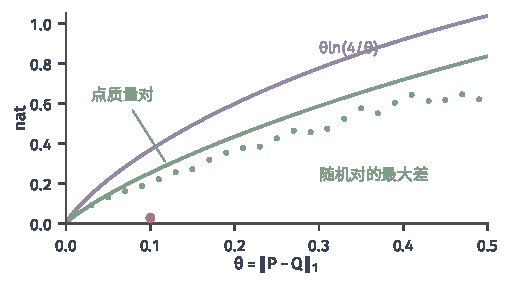
\includegraphics[width=86mm]{figures/07-probability/04-distribution-analysis/matplotlib/info-continuity/figure.pdf}
  \caption{四元字母表上熵差与$\theta=\lVert P-Q\rVert_1$。紫线为界$\theta\ln(4/\theta)$；绿线为点质量$P=(1,0,0,0)$与$Q=(1-\tfrac{\theta}{2},\tfrac{\theta}{6},\tfrac{\theta}{6},\tfrac{\theta}{6})$的熵差；绿点为$200000$对随机分布（种子$1$）在各$\theta$区间内的最大熵差。红点为四字母表与$(0.45,0.3,0.125,0.125)$：$\theta=0.1$，熵差$0.027$。}
  \label{fig:info-continuity}
\end{BookInlineFigure}

图~\ref{fig:info-continuity}比较了界与实际的熵差。离点质量很近的分布熵差最大：把一点质量从确定的结果匀给其余三个值，熵从$0$升到$h_{\mathrm{b}}(\theta/2)+\tfrac{\theta}{2}\ln3$，这条曲线在原点处的斜率同样是无穷大。随机抽取的分布对大多远离这种极端，熵差小得多。四字母表的例子中$\theta=0.1$，界为$0.1\ln40\approx0.369$，实际熵差只有$0.027$：界对最坏情形是合理的，对具体一对分布可能很宽。

\paragraph{有限组合的信息量}
互信息、条件熵在有限字母表上都是几个熵的有限组合，例如$I(X;Y)=H(X)+H(Y)-H(X,Y)$。设$(X,Y)$在$\mathcal{X}\times\mathcal{Y}$上的两个联合分布相差$\theta=\lVert P_{X,Y}-Q_{X,Y}\rVert_1\leq\tfrac12$。边缘分布的$L^{1}$距离不超过联合分布的：
\[
  \sum_x\Bigl\lvert\sum_y\bigl(p(x,y)-q(x,y)\bigr)\Bigr\rvert\leq\sum_{x,y}\lvert p(x,y)-q(x,y)\rvert=\theta.
\]
函数$t\mapsto t\ln(m/t)$在$t\leq m/\mathrm{e}$时递增，所以对边缘也可以用$\theta$代替各自的距离。对三项分别用式~\eqref{eq:info-entropy-continuity}，记$m_X=\lvert\mathcal{X}\rvert$，$m_Y=\lvert\mathcal{Y}\rvert$，得到
\begin{equation}
  \lvert I_P(X;Y)-I_Q(X;Y)\rvert\leq\theta\ln\frac{m_X}{\theta}+\theta\ln\frac{m_Y}{\theta}+\theta\ln\frac{m_Xm_Y}{\theta}.
  \label{eq:info-mi-continuity}
\end{equation}
同样的办法适用于条件熵$H(X\mid Y)=H(X,Y)-H(Y)$和条件互信息。界中的字母表大小来自所用的每一个熵。

\paragraph{无限字母表}
字母表无限时，没有类似的界。取
\[
  P_n=\bigl(1-\tfrac1n\bigr)\delta_0+\tfrac1n\operatorname{Unif}\{1,\dots,K_n\},\qquad K_n=\lceil\mathrm{e}^{n^{2}}\rceil,
\]
它与$\delta_0$的总变差是$\tfrac1n\to0$。设$X\sim P_n$，令$E=\mathbf{1}_{\{X\neq0\}}$。$E$是$X$的函数，由链式法则~\eqref{eq:info-entropy-chain-rule}先揭示$E$再揭示$X$：$E=0$时$X=0$已确定，$E=1$时$X$在$K_n$个值上均匀。于是
\[
  H(P_n)=h_{\mathrm{b}}(\tfrac1n)+\tfrac1n\ln K_n\geq\tfrac1n\cdot n^{2}=n\to\infty,
\]
而$H(\delta_0)=0$。一小份质量被摊到极多的取值上，熵就可以任意大。所以有限字母表上的连续性不能直接推广，需要额外控制质量在远处的分布方式，例如统一的尾部衰减条件。

\paragraph{连续情形与弱收敛}
对密度，弱收敛更不能保证微分熵收敛。在$[0,1]$上取密度
\[
  f_n(x)=1+\sin(2\pi nx),\qquad n=1,2,\dots.
\]
对任意连续函数$\varphi$，$\int_0^1\varphi(x)\sin(2\pi nx)\,\mathrm{d}x\to0$（Riemann–Lebesgue引理），所以$f_n$对应的分布弱收敛于$\operatorname{Unif}(0,1)$，后者的微分熵为$0$。但换元$u=nx$并利用周期性，每个$f_n$的微分熵相同：
\[
  h(f_n)=-\int_0^1(1+\sin2\pi u)\ln(1+\sin2\pi u)\,\mathrm{d}u=\ln2-1\approx-0.307.
\]
振荡越来越快，在任意固定区间上的质量与均匀分布越来越接近，但密度的高低起伏从未减小，微分熵也就停在$\ln2-1$。

\begin{BookInlineFigure}
  \centering
  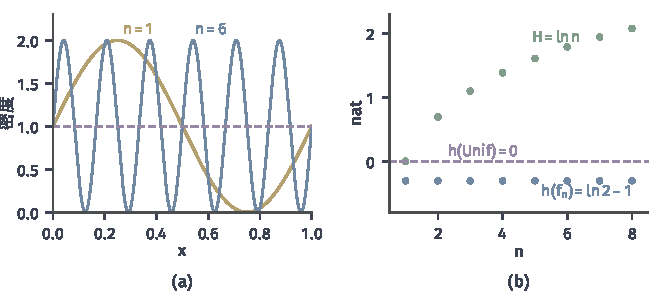
\includegraphics[width=112mm]{figures/07-probability/04-distribution-analysis/matplotlib/info-weak-entropy/figure.pdf}
  \caption{弱收敛不保证熵收敛。(a)密度$f_n(x)=1+\sin(2\pi nx)$，$n=1$（黄）与$n=6$（蓝），紫虚线为极限$\operatorname{Unif}(0,1)$的密度。(b)$h(f_n)$（蓝点，数值积分）恒为$\ln2-1$，极限的微分熵为$0$（紫虚线）；绿点为$\{\tfrac1n,\tfrac2n,\dots,1\}$上均匀分布的熵$\ln n$，它们也弱收敛于$\operatorname{Unif}(0,1)$。单位nat。}
  \label{fig:info-weak-entropy}
\end{BookInlineFigure}

图~\ref{fig:info-weak-entropy}(b)还给出了另一种失效。在$n$个等距点$\tfrac1n,\tfrac2n,\dots,1$上的均匀分布弱收敛于$\operatorname{Unif}(0,1)$，熵是$\ln n\to\infty$，而极限没有概率质量，离散熵无从谈起，只有微分熵$0$。离散分布逼近连续分布时，离散熵按式~\eqref{eq:info-quantized-entropy}的方式发散，要减去$\ln(1/n)$才有有限的极限。

所以在连续空间中谈论信息量的收敛，除了分布本身收敛，还要有关于密度的正则性（如一致有界、等度连续）与尾部的控制。弱收敛只控制有界连续函数的平均，而$-\ln f$既不有界，又随分布本身改变，不在弱收敛能控制的函数之内。


\section{本章小结}
\label{sec:info-summary}

章首问了三件事：一个随机结果平均含有多少不确定性，观测另一个变量能减少多少，以及信息不够时辨别会受到怎样的限制。本章的回答都建立在自信息$-\ln p$上。它由“罕见更意外、独立信息相加”两条要求在相差一个单位常数的意义下唯一确定，以nat或bit计只是刻度不同。

熵是自信息的平均，等于按最佳方式平均要问的是非题数（以bit计，最佳方案与熵相差不到一题）。有限字母表上熵在$0$与$\ln m$之间，两端分别对应确定结果和均匀分布，并且是概率表的凹函数；可数字母表上熵可以为无穷。对密度计算的微分熵可以为负，随坐标伸缩改变$\ln\lvert a\rvert$，它是量化熵减去精度代价$-\ln\Delta$后剩下的部分，二者的极限关系另需正则性与尾部条件。

两个变量时，联合熵不由边缘决定，条件熵是逐条件值的剩余不确定性的平均，链式法则把整体不确定性按揭示顺序分成几段。互信息定义为联合分布相对边缘乘积的KL散度，非负、对称，为零当且仅当独立，可以为无穷，也不要求密度；熵有限时它等于熵之差，由此得到条件化平均不增加熵与联合熵的次可加性。条件互信息衡量已知第三个变量后的共享信息，它与互信息之间没有固定的大小关系。

表~\ref{tab:info-summary}把本章各个量与它们回答的问题、成立条件对照列出。

\begin{BookInlineTable}
  \centering
  \caption{本章的信息量与主要条件}
  \label{tab:info-summary}
  \begin{tabular}{@{}lll@{}}
    \toprule
    量或结论 & 回答的问题 & 需要核对的条件\\
    \midrule
    $H(X)$ & 平均不确定性 & 可数时可能为无穷\\
    $h(X)$ & 密度的平均对数代价 & 可积性；依赖坐标\\
    $H(X\mid Y)$ & 观测后的剩余不确定性 & 只对平均成立\\
    $I(X;Y)$ & 共享信息 & 熵差需各项有限\\
    $H(P,Q)$ & 按参考分布付出的代价 & 零参考概率；$H(P)<\infty$\\
    数据处理 & 后处理不增加信息 & $X\perp\!\!\!\perp Z\mid Y$\\
    Fano & 辨别错误的下界 & 有限标签与猜错标准\\
    InfoNCE & 互信息的可计算下界 & 不超过$\ln N$；总体值\\
    连续性 & 分布接近时信息量接近 & 有限字母表\\
    \bottomrule
  \end{tabular}
\end{BookInlineTable}

交叉熵把平均代价分成固有部分$H(P)$与失配部分$D_{\mathrm{KL}}(P\Vert Q)$；连续时有确定意义的是后者，熵为无穷时也不能用两者之差定义KL。数据处理不等式由互信息链式法则的两种展开得到，前提是处理中的额外随机性在给定观测时与原对象独立；损失恰是条件互信息，可逆变换不损失信息，但不可逆的处理也可能不损失，判据是反向的条件独立。

信息的上界给出辨别的下界：Fano不等式用剩余不确定性限制有限标签的猜错概率，标签均匀时改写为互信息形式，成为通信中超容量不可靠、统计中候选太密无法区分的共同工具。反方向的InfoNCE用辨认真配对的总体损失给出互信息的下界，但下界受候选数$\ln N$与评分函数类的限制，下界小不能推出独立，单批样本值也不自动是下界。最后，有限字母表上熵与互信息对总变差连续，界中含有$\theta\ln(1/\theta)$与字母表大小；无限字母表或连续空间中，接近的分布可以有相差很远的信息量，弱收敛本身不保证熵收敛。

后续各章分别使用这些量。第~\ref{chap:lossless-coding}章到第~\ref{chap:rate-distortion}章研究用熵、互信息衡量的最短描述与有失真描述；第~\ref{chap:discrete-channel-capacity}章到第~\ref{chap:channel-codes}章把容量定义为互信息的最大值，并用Fano不等式证明逆定理；第~\ref{chap:dependence-measures}章把互信息与基于距离、核和离散化的依赖度量放在一起比较。


\chapter{依赖关系的度量}
\label{chap:dependence-measures}

在区间$[-1,1]$上均匀地取一个数$X$，再令$Y=X^{2}$。知道$X$就完全知道$Y$，两个变量之间的联系再紧密不过；可是它们的协方差恰好为零。若只拿相关系数去判断，会得出“两者没有关系”的结论。问题出在相关系数只检查一种特定的联系：$Y$是否随$X$线性地增减。抛物线左半支下降、右半支上升，两种趋势正好抵消。

要回答“$X$与$Y$是否独立”，需要比较整个联合分布$P_{(X,Y)}$与边缘乘积$P_X\otimes P_Y$。两者相等就是独立；不等时，差别可以从多个角度去量：观测一个变量后另一个变量的不确定性减少了多少，成对距离是否一起变化，联合分布与边缘乘积在某个核空间里相距多远，把取值装进有限个格子后格子标签之间是否还有关联。每个角度给出一个依赖度量，它们的零值、取值范围、对坐标变换的反应和需要的参数各不相同。

第一节用抛物线和几个零相关的例子把共同问题提出来，区分三件事：零值能否刻画独立，非零数值怎样随依赖变化，以及能否从有限样本可靠地判断。后面四节依次研究四类度量。互信息直接回用第~\ref{chap:information-measures}章的定义，这里关心它对一一变换的不变性，以及确定关系为什么给出无穷大。距离协方差用特征函数之差的加权积分定义，它能写成成对距离的期望，归一化后得到距离相关。HSIC把联合分布与边缘乘积放进乘积核的RKHS，用第~\ref{chap:distribution-comparison}章的MMD比较。离散化评分先把取值分格，再对格子标签计算互信息。最后一节把这些量放在同一组分布上比较。

全章贯穿三个例子：三点抛物线（$X$在$\{-1,0,1\}$上等可能，$Y=X^{2}$），连续抛物线（$X\sim\operatorname{Unif}(-1,1)$，$Y=X^{2}$，必要时加噪声），以及相关系数为$\rho$的标准二元高斯分布。本章讨论的都是给定联合分布时的总体量；由样本估计这些量、校准估计误差和检验独立性，属于统计推断的问题。

\section{从相关到独立}
\label{sec:dep-correlation-to-independence}

协方差为零时，两个变量还可能有多强的联系？先把开头的抛物线算清楚。

\paragraph{零协方差的抛物线}
设$X\sim\operatorname{Unif}(-1,1)$，$Y=X^{2}$。$X$的密度在$[-1,1]$上为$1/2$，奇数次矩为零，于是
\[
  \mathbb{E}[X]=0,\qquad \mathbb{E}[X^{3}]=\frac12\int_{-1}^{1}x^{3}\,\mathrm{d}x=0 .
\]
代入协方差的定义，得到
\[
  \operatorname{Cov}(X,Y)=\mathbb{E}[XY]-\mathbb{E}[X]\,\mathbb{E}[Y]=\mathbb{E}[X^{3}]-0=0 .
\]
$X$与$Y$不相关。但它们并不独立：事件$A=\{\lvert X\rvert\leq1/2\}$发生时一定有$Y\leq1/4$，所以
\[
  \mathbb{P}\bigl(\lvert X\rvert\leq\tfrac12,\ Y>\tfrac14\bigr)=0 .
\]
若两者独立，这个概率应当等于两个边缘概率的乘积，
\[
  \mathbb{P}\bigl(\lvert X\rvert\leq\tfrac12\bigr)\,\mathbb{P}\bigl(Y>\tfrac14\bigr)=\frac12\cdot\frac12=\frac14 .
\]

图~\ref{fig:dep-parabola-joint-product}把这两个数画了出来。左图是$(X,Y)$的样本，全部落在抛物线上；右图是“假装独立”的样本：$X$与$Y$各按自己的边缘分布抽取，但彼此独立。两幅图的横坐标分布相同，纵坐标分布也相同，差别只在点怎样配对。红框里的事件在左图中没有点，在右图中约占四分之一。

\begin{BookInlineFigure}
  \centering
  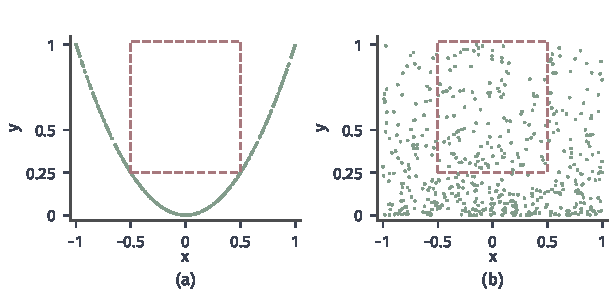
\includegraphics[width=104mm]{figures/07-probability/04-distribution-analysis/matplotlib/dep-parabola-joint-product/figure.pdf}
  \caption{同样的边缘，不同的配对。(a)$X\sim\operatorname{Unif}(-1,1)$，$Y=X^{2}$的$500$个样本（绿）；(b)边缘乘积$P_X\otimes P_Y$的$500$个样本，即把$X$与一个独立复制$X'$的平方配对。红色虚线框是事件$\{\lvert x\rvert\leq1/2,\ y>1/4\}$，其概率在(a)中为$0$，在(b)中为$1/4$（样本中占$0.248$）。种子$719$。}
  \label{fig:dep-parabola-joint-product}
\end{BookInlineFigure}

\paragraph{协方差只是一个测试}
协方差为零说的是$\mathbb{E}[(X-\mathbb{E}X)(Y-\mathbb{E}Y)]=0$，即一对特定函数$x\mapsto x$、$y\mapsto y$的乘积在联合分布下的期望，与在边缘乘积下的期望相同。独立要求的多得多：对一切有界可测函数$f,g$，
\begin{equation}
  \mathbb{E}\bigl[f(X)\,g(Y)\bigr]=\mathbb{E}\bigl[f(X)\bigr]\,\mathbb{E}\bigl[g(Y)\bigr],
  \label{eq:dep-independence-test-functions}
\end{equation}
这等价于联合分布等于边缘乘积，
\begin{equation}
  P_{(X,Y)}=P_X\otimes P_Y .
  \label{eq:dep-independence}
\end{equation}
取$f,g$为示性函数，式~\eqref{eq:dep-independence-test-functions}就是矩形事件上的乘积公式，它确定两个分布相等；反过来，由矩形事件的乘积公式经简单函数逼近得到一般有界$f,g$的情形，这正是第~\ref{chap:probability-spaces}章建立独立性时走过的路。

协方差是式~\eqref{eq:dep-independence-test-functions}中只取一对线性函数的结果，换一对函数就能看出抛物线的依赖。取$f(x)=x^{2}$，$g(y)=y$，由$\mathbb{E}[X^{2}]=1/3$与$\mathbb{E}[X^{4}]=1/5$，
\[
  \operatorname{Cov}\bigl(X^{2},Y\bigr)=\operatorname{Var}\bigl(X^{2}\bigr)=\frac15-\frac19=\frac{4}{45}>0 .
\]
所以“协方差为零”只排除了一种线性的联系。这一点在第~\ref{chap:random-vectors}章已经见过：不相关不等于独立。

\paragraph{零相关的几种形状}
图~\ref{fig:dep-zero-correlation-shapes}收集了几种协方差为零的联合分布。(b)中$Y=SX$，$S$是与$X$独立、等可能取$\pm1$的随机符号，协方差是$\mathbb{E}[S]\,\mathbb{E}[X^{2}]=0$，可是$\lvert Y\rvert=\lvert X\rvert$。(c)是单位圆周上的均匀分布，两个坐标满足$X^{2}+Y^{2}=1$。只有(d)两个坐标独立。四幅图的相关系数都是零，相关系数无法把(d)与前三幅区分开。

\begin{BookInlineFigure}
  \centering
  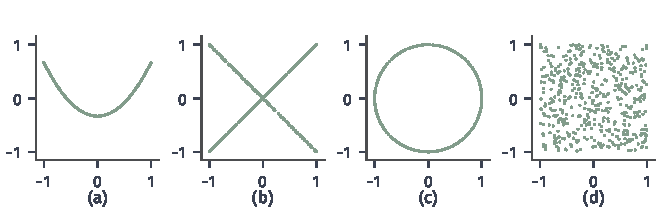
\includegraphics[width=112mm]{figures/07-probability/04-distribution-analysis/matplotlib/dep-zero-correlation-shapes/figure.pdf}
  \caption{协方差都为零的四个联合分布，各$500$个样本（种子$719$）。(a)$X\sim\operatorname{Unif}(-1,1)$与$X^{2}-1/3$；(b)$X$与$SX$，$S$为独立随机符号；(c)单位圆周上的均匀分布；(d)两个独立的$\operatorname{Unif}(-1,1)$。前三个都不独立。}
  \label{fig:dep-zero-correlation-shapes}
\end{BookInlineFigure}

\paragraph{相关足够的两种情形}
有两类联合分布，零相关确实等价于独立。一类是联合高斯向量，第~\ref{chap:multivariate-distributions}章已经证明。另一类是两个二值变量。设$X,Y$都取值于$\{0,1\}$，记$p=\mathbb{P}(X=1)$，$q=\mathbb{P}(Y=1)$。由$XY=\mathbf{1}_{\{X=1,Y=1\}}$，
\[
  \mathbb{P}(X=1,\,Y=1)-pq=\mathbb{E}[XY]-\mathbb{E}[X]\,\mathbb{E}[Y]=\operatorname{Cov}(X,Y).
\]
其余三个格子由边缘减出来。例如$\mathbb{P}(X=1,Y=0)=p-\mathbb{P}(X=1,Y=1)$，它与$p(1-q)$之差是$-\operatorname{Cov}(X,Y)$。所以$2\times2$概率表的四个格子与独立时的乘积只差$\pm\operatorname{Cov}(X,Y)$，协方差为零时四个格子都分解成乘积。二值变量只有一个“自由度”可以偏离独立，协方差恰好量的就是它。取值多于两个时，偏离独立的方向不止一个，单个协方差看不全。

\paragraph{三点抛物线}
最小的反例只需要三个点。设$X$在$\{-1,0,1\}$上等可能，$Y=X^{2}$。$(X,Y)$等可能取$(-1,1)$、$(0,0)$、$(1,1)$三个值，边缘为
\[
  \mathbb{P}(X=x)=\tfrac13\ (x=-1,0,1),\qquad \mathbb{P}(Y=1)=\tfrac23,\qquad \mathbb{P}(Y=0)=\tfrac13 .
\]
协方差仍是$\mathbb{E}[X^{3}]=\frac13(-1+0+1)=0$。图~\ref{fig:dep-three-point-tables}把联合概率表与边缘乘积表并排放在一起：联合表有三个格子为零，乘积表六个格子都是正数。这个例子取值有限，所有度量都能手算，后面每一节都会回到它。

\begin{BookInlineFigure}
  \centering
  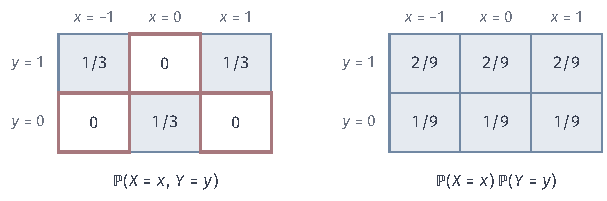
\includegraphics[width=102.8mm]{figures/07-probability/04-distribution-analysis/tikz/dep-three-point-tables/figure.pdf}
  \caption{三点抛物线。左：联合概率表$\mathbb{P}(X=x,Y=y)$，浅蓝格子有正质量，红框标出联合表为零而乘积表为正的三个格子。右：边缘乘积$\mathbb{P}(X=x)\,\mathbb{P}(Y=y)$，其中$\mathbb{P}(Y=1)=2/3$，$\mathbb{P}(Y=0)=1/3$。}
  \label{fig:dep-three-point-tables}
\end{BookInlineFigure}

\paragraph{依赖度量要回答的三件事}
于是共同的问题是：$P_{(X,Y)}$离$P_X\otimes P_Y$有多远。把联合分布映成一个非负数的泛函，称为\term{依赖度量}（dependence measure）。评价一个依赖度量，要把三件不同的事分开。

第一件是零值判据：度量为零是否当且仅当独立。协方差在一般分布上做不到，在联合高斯和二值变量上做得到；本章的互信息、距离协方差、高斯核HSIC在各自的条件下都做得到。第二件是非零数值的含义：依赖变强时数值是否增大，有没有上界，对重新标记、平移、缩放、单调变换是否敏感，需要预先选哪些参数。这一件没有统一答案，不同度量给同一对分布排出的强弱次序可以相反。第三件是有限样本：只观测到$n$对数据时，能否可靠地判断度量是否为零，误差有多大。

本章的定义都是总体量，只回答前两件事。第三件要另外分析估计量的偏差、方差和分布，即使度量的零值完全刻画独立，样本上算出的一个正数也不等于证明了依赖，这部分由统计推断承担，可参考\BookChapterRef{chap:nonparametric-inference}{卷八第2章“非参数分布与函数推断”}。


\section{互信息作为依赖量}
\label{sec:dep-mutual-information}

第~\ref{chap:information-measures}章已经给出一个直接比较式~\eqref{eq:dep-independence}两边的量。设$X,Y$分别取值于可测空间$\mathcal{X},\mathcal{Y}$，互信息定义为联合分布相对边缘乘积的KL散度，
\begin{equation}
  I(X;Y)=D_{\mathrm{KL}}\bigl(P_{(X,Y)}\,\Vert\,P_X\otimes P_Y\bigr)\in[0,\infty].
  \label{eq:dep-mi}
\end{equation}
按第~\ref{chap:distribution-comparison}章的约定，若$P_{(X,Y)}$不绝对连续于$P_X\otimes P_Y$，KL散度取$+\infty$。那里也证明了KL散度非负、且为零当且仅当两个分布相同，所以
\[
  I(X;Y)=0\iff P_{(X,Y)}=P_X\otimes P_Y\iff X\text{与}Y\text{独立}.
\]
零值判据不需要任何矩条件，也不需要$\mathcal{X},\mathcal{Y}$是欧氏空间。在离散情形，式~\eqref{eq:dep-mi}写成概率表上的求和
\[
  I(X;Y)=\sum_{x,y}p_{X,Y}(x,y)\ln\frac{p_{X,Y}(x,y)}{p_X(x)\,p_Y(y)},
\]
零概率的格子按$0\ln0=0$不计入。

用三点抛物线算一遍。联合表只有三个正格子，每个概率为$1/3$。格子$(\pm1,1)$处边缘乘积为$\frac13\cdot\frac23=\frac29$，格子$(0,0)$处为$\frac13\cdot\frac13=\frac19$。代入求和式，
\[
  I(X;Y)=2\cdot\frac13\ln\frac{1/3}{2/9}+\frac13\ln\frac{1/3}{1/9}=\frac23\ln\frac32+\frac13\ln3 .
\]
整理成一个数，
\[
  I(X;Y)=\ln3-\tfrac23\ln2\approx0.637\ \text{nat}.
\]
它恰好等于$Y$的熵$H(Y)=\frac13\ln3+\frac23\ln\frac32$：$Y$由$X$确定，观测$X$后$Y$的不确定性全部消失，减少量就是$Y$原有的不确定性。

互信息的熵差表示、链式法则和计算下界都在第~\ref{chap:information-measures}章，这里不再重复。下面关心的是：把互信息当作依赖的强弱刻度时，它对坐标变换怎样反应，数值能大到什么程度。

\subsection{变换不变性}
\label{sec:dep-mi-invariance}

把$Y$的两个取值$0,1$改名为“短”“长”，或者把温度从摄氏度换成华氏度，两个变量之间的依赖不应当改变。互信息正好如此。所用的工具是第~\ref{chap:information-measures}章的数据处理不等式：若$Z$只通过$Y$依赖$X$，即给定$Y$时$X$与$Z$条件独立，则$I(X;Z)\leq I(X;Y)$。$Z=g(Y)$由$Y$确定，这个条件自动成立。

\begin{theorem}[互信息的变换性质]
\label{thm:dep-mi-invariance}
设$f:\mathcal{X}\to\mathcal{X}'$与$g:\mathcal{Y}\to\mathcal{Y}'$可测。
\begin{enumerate}
  \item 局部处理不增加互信息：
  \begin{equation}
    I\bigl(f(X);g(Y)\bigr)\leq I(X;Y).
    \label{eq:dep-mi-processing}
  \end{equation}
  \item 若$f$与$g$都是双向可测的一一映射（逆映射也可测），则
  \begin{equation}
    I\bigl(f(X);g(Y)\bigr)=I(X;Y).
    \label{eq:dep-mi-invariance}
  \end{equation}
\end{enumerate}
\end{theorem}

\begin{proof}
先处理$Y$一侧。$g(Y)$是$Y$的函数，由数据处理不等式，$I(X;g(Y))\leq I(X;Y)$。互信息关于两个变量对称，对$X$一侧同样有$I(f(X);g(Y))\leq I(X;g(Y))$。两步相连，
\[
  I\bigl(f(X);g(Y)\bigr)\leq I\bigl(X;g(Y)\bigr)\leq I(X;Y),
\]
这就是式~\eqref{eq:dep-mi-processing}。

若$f,g$双向可测且一一，则$X=f^{-1}(f(X))$、$Y=g^{-1}(g(Y))$，对变量$f(X),g(Y)$与可测映射$f^{-1},g^{-1}$再用一次式~\eqref{eq:dep-mi-processing}，
\[
  I(X;Y)=I\bigl(f^{-1}(f(X));\,g^{-1}(g(Y))\bigr)\leq I\bigl(f(X);g(Y)\bigr).
\]
与第一部分相反方向的不等式合起来，得到式~\eqref{eq:dep-mi-invariance}。
\end{proof}

\paragraph{改名与改坐标}
在三点抛物线中，把$X$的取值$-1,0,1$换成$-1,0,5$，或把$Y$的取值$0,1$换成$0,100$，概率表的格局完全不变，互信息仍是$\ln3-\frac23\ln2$。互信息只看“哪些取值一起出现、各占多少概率”，不看取值之间相距多远。这既是长处也是局限：它不受单位和刻度影响，但也不反映“$Y$随$X$变化了多少”。

连续变量的例子是标准二元高斯$(X,Y)$，相关系数$\rho=0.5$，协方差矩阵$\bm{\Sigma}$的对角元为$1$、非对角元为$\rho$。$d$维高斯向量的微分熵是$\frac12\ln\bigl((2\pi\mathrm{e})^{d}\det\bm{\Sigma}\bigr)$，用第~\ref{chap:information-measures}章的熵差表示$I(X;Y)=h(X)+h(Y)-h(X,Y)$，常数项相消，只剩
\begin{equation}
  I(X;Y)=-\tfrac12\ln\det\bm{\Sigma}=-\tfrac12\ln(1-\rho^{2}).
  \label{eq:dep-gauss-mi}
\end{equation}
$\rho=0.5$时它等于$-\frac12\ln0.75\approx0.144$ nat。
对两个坐标分别作严格增变换$x\mapsto\mathrm{e}^{x}$，得到对数正态向量$(\mathrm{e}^{X},\mathrm{e}^{Y})$。它的相关系数由高斯的矩母函数算出。$X+Y$的方差为$2+2\rho$，所以
\[
  \mathbb{E}[\mathrm{e}^{X}]=\mathrm{e}^{1/2},\qquad \mathbb{E}[\mathrm{e}^{2X}]=\mathrm{e}^{2},\qquad \mathbb{E}[\mathrm{e}^{X+Y}]=\mathrm{e}^{1+\rho}.
\]
于是
\[
  \operatorname{Corr}\bigl(\mathrm{e}^{X},\mathrm{e}^{Y}\bigr)=\frac{\mathrm{e}^{1+\rho}-\mathrm{e}}{\mathrm{e}^{2}-\mathrm{e}}=\frac{\mathrm{e}^{\rho}-1}{\mathrm{e}-1}\approx0.378 .
\]
相关系数从$0.5$降到$0.378$，互信息由定理~\ref{thm:dep-mi-invariance}保持$0.144$不变。

\paragraph{只依赖Copula}
再换一种坐标：用分布函数把两个分量都送到$(0,1)$上，$(U,V)=(\Phi(X),\Phi(Y))$。这正是第~\ref{chap:distribution-families}章的概率积分变换，$(U,V)$的分布是$\rho=0.5$的高斯Copula。$\Phi$连续且严格增，是双向可测的一一映射，所以$I(U;V)=I(X;Y)$。一般地，若$X,Y$为实值、分布函数$F_X,F_Y$连续，则$U=F_X(X)$与$X$只差一个零概率事件上的取值（$X=Q_X(U)$几乎必然成立，$Q_X$为分位数函数），同样两次运用数据处理得到
\[
  I(X;Y)=I\bigl(F_X(X);F_Y(Y)\bigr).
\]
连续边缘下，互信息只依赖Copula，与边缘分布无关；若Copula有密度$c$，它就是$\int_{[0,1]^{2}}c\ln c$。图~\ref{fig:dep-mi-coordinates}把同一组高斯样本画在三种坐标下：点云形状差别很大，相关系数分别为$0.5$、$0.378$、$0.483$，互信息都是$0.144$。

\begin{BookInlineFigure}
  \centering
  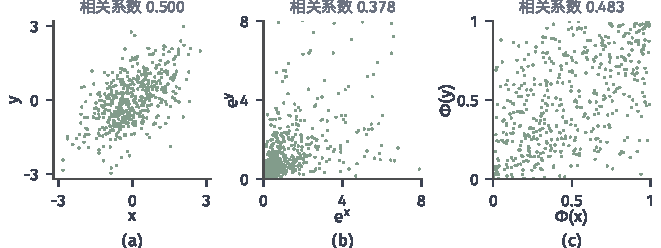
\includegraphics[width=112mm]{figures/07-probability/04-distribution-analysis/matplotlib/dep-mi-coordinates/figure.pdf}
  \caption{同一组标准二元高斯样本（$\rho=0.5$，$500$个，种子$719$）在三种坐标下。(a)原坐标；(b)$(\mathrm{e}^{x},\mathrm{e}^{y})$，有$15$个点超出画框；(c)$(\Phi(x),\Phi(y))$，即高斯Copula。图上方是各自的相关系数$\rho$、$(\mathrm{e}^{\rho}-1)/(\mathrm{e}-1)$与$(6/\pi)\arcsin(\rho/2)$；三者的互信息都是$-\frac12\ln0.75\approx0.144$。}
  \label{fig:dep-mi-coordinates}
\end{BookInlineFigure}

\paragraph{不可逆的处理}
若$f$不是一一的，式~\eqref{eq:dep-mi-processing}一般是严格不等式。在三点抛物线中只保留$X$是否为正，令$B=\mathbf{1}_{\{X>0\}}$。$B=1$时$X=1$，$Y=1$确定；$B=0$（概率$2/3$）时$X$等可能为$-1$或$0$，$Y$等可能为$1$或$0$，剩下$\ln2$的不确定性。于是
\[
  H(Y\mid B)=\tfrac23\ln2,\qquad I(B;Y)=H(Y)-H(Y\mid B)=\ln3-\tfrac43\ln2\approx0.174 .
\]
从$0.637$降到$0.174$：把$-1$和$0$合并以后，原来能区分的情形不再能区分。如果只合并$X$的$-1$与$1$，即改用$\lvert X\rvert$，那么$Y=\lvert X\rvert$仍由它确定，互信息不变。是否损失信息，看被合并的取值对另一个变量是否“有区别”。

\subsection{确定关系与无穷信息}
\label{sec:dep-mi-infinite}

三点抛物线的互信息是有限的$0.637$，那么连续抛物线$X\sim\operatorname{Unif}(-1,1)$，$Y=X^{2}$呢？$Y$同样由$X$确定，但它有不可数多个取值，“观测$X$后消除的不确定性”没有上限。

先看直观图景。联合分布的全部质量都在抛物线$y=x^{2}$上，这条曲线在平面上面积为零；边缘乘积则把质量摊在整个矩形$[-1,1]\times[0,1]$上，密度是$\frac12\cdot\frac{1}{2\sqrt{y}}$。在曲线周围取一条宽为$2\varepsilon$的带子$\{\lvert y-x^{2}\rvert\leq\varepsilon\}$。联合分布给它概率$1$，边缘乘积给它的概率记为$q_\varepsilon$，它随$\varepsilon\to0$趋于零。只记录“是否落在带子里”这个二值标签，由数据处理不等式，
\[
  I(X;Y)\geq D_{\mathrm{KL}}\bigl(\operatorname{Bern}(1)\,\Vert\,\operatorname{Bern}(q_\varepsilon)\bigr)=\ln\frac{1}{q_\varepsilon}.
\]
数值计算给出$q_{0.05}\approx0.134$，$q_{0.01}\approx0.035$，相应的下界约为$2.01$与$3.35$。带子越窄，下界越大，图~\ref{fig:dep-graph-band}画出了这一过程。

\begin{BookInlineFigure}
  \centering
  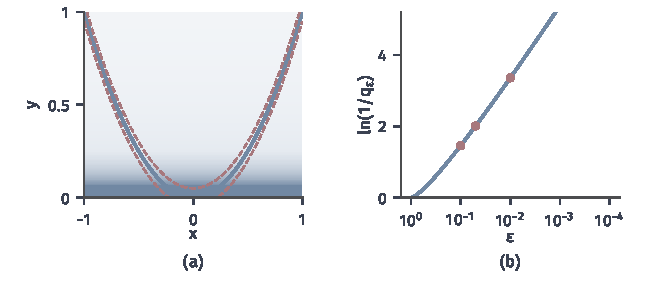
\includegraphics[width=110mm]{figures/07-probability/04-distribution-analysis/matplotlib/dep-graph-band/figure.pdf}
  \caption{质量在曲线上与质量摊开。(a)连续抛物线的边缘乘积密度$1/(4\sqrt{y})$（白到蓝，大于$1$的部分截断显示）；蓝线是联合分布的全部质量所在的曲线$y=x^{2}$，红色虚线围出带子$\lvert y-x^{2}\rvert\leq0.05$。(b)带子在边缘乘积下的概率$q_\varepsilon$给出的下界$\ln(1/q_\varepsilon)$，横轴向右$\varepsilon$减小；红点为$\varepsilon=0.1,0.05,0.01$，对应$1.46$、$2.01$、$3.35$。}
  \label{fig:dep-graph-band}
\end{BookInlineFigure}

下面的定理把“曲线面积为零”换成边缘乘积给图像零概率，给出一般结论。这里要求取值空间是标准Borel空间（第~\ref{chap:conditional-distributions}章引入，欧氏空间及其Borel子集都是），它保证了函数图像可测。

\begin{theorem}[确定关系的互信息]
\label{thm:dep-mi-infinite}
设$\mathcal{X},\mathcal{Y}$是标准Borel空间，$f:\mathcal{X}\to\mathcal{Y}$可测，$Y=f(X)$。若$Y$的分布无原子，即$\mathbb{P}(Y=y)=0$对每个$y\in\mathcal{Y}$成立，则
\begin{equation}
  I\bigl(X;f(X)\bigr)=+\infty .
  \label{eq:dep-mi-infinite}
\end{equation}
\end{theorem}

\begin{proof}
考虑$f$的图像$G=\{(x,y):y=f(x)\}$。标准Borel空间的对角线$\Delta=\{(y,y)\}$是$\mathcal{Y}\times\mathcal{Y}$中的可测集，而$G$是$\Delta$在可测映射$(x,y)\mapsto(f(x),y)$下的原像，所以$G$可测。

联合分布把全部质量放在$G$上：
\[
  P_{(X,Y)}(G)=\mathbb{P}\bigl(f(X)=Y\bigr)=1 .
\]
再算边缘乘积给$G$的概率。由乘积测度的截面公式（Tonelli定理），先固定$x$，截面$\{y:(x,y)\in G\}$只有一个点$f(x)$，于是
\[
  (P_X\otimes P_Y)(G)=\int_{\mathcal{X}}P_Y\bigl(\{f(x)\}\bigr)\,P_X(\mathrm{d}x)=0 ,
\]
最后一步用了$P_Y$无原子。一个集合在$P_X\otimes P_Y$下概率为零、在$P_{(X,Y)}$下概率为一，所以$P_{(X,Y)}$不绝对连续于$P_X\otimes P_Y$，按约定式~\eqref{eq:dep-mi}中的KL散度为$+\infty$。
\end{proof}

定理中两个条件各有作用。无原子保证了边缘乘积给图像零概率；若$Y$有原子，例如三点抛物线，图像的乘积概率为正，互信息有限。标准Borel保证图像可测，从而“质量全在图像上”有意义。函数$f$本身不需要连续或单调：$f(x)=x^{2}$不是一一的，结论照样成立。

\paragraph{有限与无穷的分界}
离散情形的对照是：若$Y=f(X)$只取有限多个值，那么给定$X$后$Y$没有不确定性，
\[
  I\bigl(X;f(X)\bigr)=H\bigl(f(X)\bigr)\leq\ln\lvert f(\mathcal{X})\rvert ,
\]
其中$\lvert f(\mathcal{X})\rvert$是取值个数。三点抛物线$H(Y)=0.637<\ln2$就是这种情形。可数无穷多个取值时，$H(f(X))$可以已经是无穷大；不可数且无原子时，定理~\ref{thm:dep-mi-infinite}说它一定是无穷大。所以互信息没有一个对所有分布都成立的有限上界，它的数值本身不能直接归一化到$[0,1]$。

加一点噪声，互信息又变成有限的。令$Y=X^{2}+\sigma Z$，$Z\sim\mathcal{N}(0,1)$与$X$独立。给定$X=x$时$Y\sim\mathcal{N}(x^{2},\sigma^{2})$，条件微分熵是$\frac12\ln(2\pi\mathrm{e}\sigma^{2})$，所以
\[
  I(X;Y)=h(Y)-\tfrac12\ln(2\pi\mathrm{e}\sigma^{2}),
\]
其中$h(Y)$对$Y$的密度（$X^{2}$的分布与$\mathcal{N}(0,\sigma^{2})$的卷积）数值积分得到。$\sigma=0.2$时约为$0.555$，$\sigma=0.1$时约为$1.03$。$\sigma\to0$时$h(Y)$趋于$X^{2}$的微分熵，而噪声项$-\frac12\ln(2\pi\mathrm{e}\sigma^{2})$像$\ln(1/\sigma)$那样增长，互信息随之发散。高斯情形的$-\frac12\ln(1-\rho^{2})$在$\lvert\rho\rvert\to1$时同样发散。图~\ref{fig:dep-mi-noise}把两种发散画在一起。

\begin{BookInlineFigure}
  \centering
  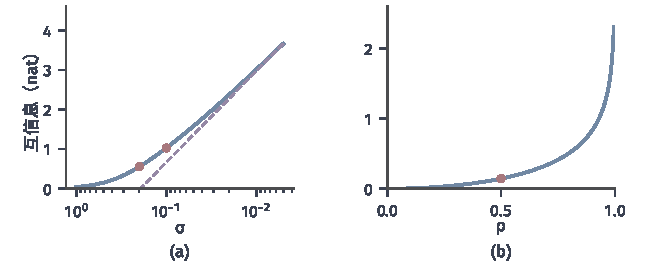
\includegraphics[width=110mm]{figures/07-probability/04-distribution-analysis/matplotlib/dep-mi-noise/figure.pdf}
  \caption{互信息向无穷大发散。(a)$I(X;X^{2}+\sigma Z)$随$\sigma$减小（横轴向右）而增大，蓝线由$h(Y)-\frac12\ln(2\pi\mathrm{e}\sigma^{2})$数值积分得到；紫色虚线是斜率与$\ln(1/\sigma)$相同的参考线；红点为$\sigma=0.2,0.1$，数值约$0.555$、$1.03$。(b)标准二元高斯的$I=-\frac12\ln(1-\rho^{2})$，红点为$\rho=0.5$处的$0.144$。}
  \label{fig:dep-mi-noise}
\end{BookInlineFigure}

\paragraph{下界不是数值}
真实互信息可以无穷大，计算上常用的却是有限的下界。第~\ref{chap:information-measures}章的InfoNCE下界在$N$个候选时不超过$\ln N$：对连续抛物线，$N=16$时它至多给出$\ln16\approx2.77$，而真实值是$+\infty$。下界给出“至少有这么多信息”，不能读成“信息就这么多”；两个分布的下界大小次序，也不一定是它们真实互信息的次序。


\section{距离协方差}
\label{sec:dep-distance-covariance}

互信息不看取值之间的距离，也没有有限上界。对欧氏空间中的随机向量，我们想要另一种度量：它的零值仍然刻画独立，数值又能用成对距离直接计算，并且有界。出发点是第~\ref{chap:weak-convergence-of-distributions}章的特征函数。设$\bm{X}$取值于$\mathbb{R}^{p}$，$\bm{Y}$取值于$\mathbb{R}^{q}$，联合特征函数为
\[
  \phi_{\bm{X},\bm{Y}}(\bm{t},\bm{s})=\mathbb{E}\bigl[\mathrm{e}^{\mathrm{i}\langle\bm{t},\bm{X}\rangle+\mathrm{i}\langle\bm{s},\bm{Y}\rangle}\bigr],\qquad \bm{t}\in\mathbb{R}^{p},\ \bm{s}\in\mathbb{R}^{q}.
\]
边缘乘积$P_{\bm{X}}\otimes P_{\bm{Y}}$的特征函数是$\phi_{\bm{X}}(\bm{t})\phi_{\bm{Y}}(\bm{s})$：在乘积空间上取独立的$\tilde{\bm{X}}\sim P_{\bm{X}}$、$\tilde{\bm{Y}}\sim P_{\bm{Y}}$，期望分解成乘积。特征函数确定分布，所以独立等价于两个特征函数处处相等。依赖的大小就用它们之差
\[
  \Delta(\bm{t},\bm{s})=\phi_{\bm{X},\bm{Y}}(\bm{t},\bm{s})-\phi_{\bm{X}}(\bm{t})\,\phi_{\bm{Y}}(\bm{s})
\]
在所有频率上的加权平方积分来量。关键在于选什么权重。

\subsection{定义与独立性}
\label{sec:dep-dcov-definition}

权重要满足三点：处处为正，才不会漏掉某个频段的差别；积分有限；最好还能把积分算回原来的取值空间。下面这个积分恒等式说明，幂次权重$\lVert\bm{t}\rVert_2^{-(d+1)}$把“频率空间里的$1-\cos$”变成“取值空间里的距离”。

\begin{lemma}[余弦积分与距离]
\label{lem:dep-cos-integral}
对$d\geq1$，记
\begin{equation}
  c_d=\int_{\mathbb{R}^{d}}\frac{1-\cos t_1}{\lVert\bm{t}\rVert_2^{d+1}}\,\mathrm{d}\bm{t},
  \label{eq:dep-cd}
\end{equation}
其中$t_1$是$\bm{t}$的第一个坐标。则$0<c_d<\infty$，$c_1=\pi$，并且对每个$\bm{x}\in\mathbb{R}^{d}$，
\begin{equation}
  \int_{\mathbb{R}^{d}}\frac{1-\cos\langle\bm{t},\bm{x}\rangle}{\lVert\bm{t}\rVert_2^{d+1}}\,\mathrm{d}\bm{t}=c_d\,\lVert\bm{x}\rVert_2 .
  \label{eq:dep-cos-integral}
\end{equation}
\end{lemma}

\begin{proof}
先证式~\eqref{eq:dep-cd}有限。在单位球内，
\[
  1-\cos t_1\leq\tfrac12t_1^{2}\leq\tfrac12\lVert\bm{t}\rVert_2^{2},
\]
被积函数不超过$\frac12\lVert\bm{t}\rVert_2^{1-d}$。用极坐标，$\mathbb{R}^{d}$中半径$r$的球面面积与$r^{d-1}$成正比，
\[
  \int_{\lVert\bm{t}\rVert_2\leq1}\lVert\bm{t}\rVert_2^{1-d}\,\mathrm{d}\bm{t}\ \propto\ \int_0^1r^{1-d}\,r^{d-1}\,\mathrm{d}r=1 .
\]
在单位球外，由$1-\cos t_1\leq2$，被积函数不超过$2\lVert\bm{t}\rVert_2^{-d-1}$，对应的径向积分为$\int_1^\infty r^{-2}\,\mathrm{d}r=1$。两部分都有限。被积函数非负，且在$t_1\notin2\pi\mathbb{Z}$处为正，所以$c_d>0$。

再证式~\eqref{eq:dep-cos-integral}。$\bm{x}=\bm{0}$时两边都是零。$\bm{x}\neq\bm{0}$时，取正交矩阵$\bm{R}$使$\bm{R}\bm{x}=\lVert\bm{x}\rVert_2\bm{e}_1$，作代换$\bm{u}=\bm{R}\bm{t}$。正交变换保持体积与范数，并且
\[
  \langle\bm{t},\bm{x}\rangle=\langle\bm{R}\bm{t},\bm{R}\bm{x}\rangle=\lVert\bm{x}\rVert_2u_1 ,
\]
所以左边变为
\[
  \int_{\mathbb{R}^{d}}\frac{1-\cos(\lVert\bm{x}\rVert_2u_1)}{\lVert\bm{u}\rVert_2^{d+1}}\,\mathrm{d}\bm{u}.
\]
再令$\bm{v}=\lVert\bm{x}\rVert_2\bm{u}$，体积元与分母分别变为
\[
  \mathrm{d}\bm{u}=\lVert\bm{x}\rVert_2^{-d}\,\mathrm{d}\bm{v},\qquad \lVert\bm{u}\rVert_2^{d+1}=\lVert\bm{x}\rVert_2^{-d-1}\lVert\bm{v}\rVert_2^{d+1},
\]
积分变为
\[
  \lVert\bm{x}\rVert_2^{d+1}\cdot\lVert\bm{x}\rVert_2^{-d}\int_{\mathbb{R}^{d}}\frac{1-\cos v_1}{\lVert\bm{v}\rVert_2^{d+1}}\,\mathrm{d}\bm{v}=c_d\,\lVert\bm{x}\rVert_2 .
\]

最后求$c_1$。三角形密度$f(x)=(1-\lvert x\rvert)^{+}$的特征函数是
\[
  \phi(t)=2\int_0^1(1-x)\cos(tx)\,\mathrm{d}x=\frac{2(1-\cos t)}{t^{2}},
\]
最后一步用分部积分：
\[
  \int_0^1(1-x)\cos(tx)\,\mathrm{d}x=\Bigl[(1-x)\frac{\sin tx}{t}\Bigr]_0^1+\int_0^1\frac{\sin tx}{t}\,\mathrm{d}x=\frac{1-\cos t}{t^{2}}.
\]$\phi$非负可积，由第~\ref{chap:weak-convergence-of-distributions}章的反演公式在$x=0$处，
\[
  1=f(0)=\frac{1}{2\pi}\int_{-\infty}^{\infty}\phi(t)\,\mathrm{d}t=\frac1\pi\int_{-\infty}^{\infty}\frac{1-\cos t}{t^{2}}\,\mathrm{d}t ,
\]
所以$c_1=\pi$。
\end{proof}

一般维数的常数是$c_d=\pi^{(d+1)/2}/\Gamma\bigl((d+1)/2\bigr)$，后面只用到它有限且为正，不需要具体数值。图~\ref{fig:dep-cos-kernel}画出$d=1$的被积函数：$x=2$的曲线在原点附近高出四倍、宽度减半，总面积恰好加倍。

\begin{BookInlineFigure}
  \centering
  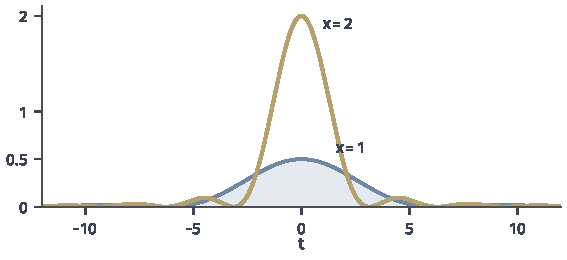
\includegraphics[width=96mm]{figures/07-probability/04-distribution-analysis/matplotlib/dep-cos-kernel/figure.pdf}
  \caption{引理~\ref{lem:dep-cos-integral}在$d=1$时的被积函数$(1-\cos tx)/t^{2}$。蓝线与浅蓝面积对应$x=1$，黄线对应$x=2$；两者在实轴上的积分分别为$\pi$与$2\pi$，与$\lvert x\rvert$成正比（数值积分在$[-4000,4000]$上得$3.1401$与$6.2787$，截去的尾部不超过$2/4000$与$4/4000$）。}
  \label{fig:dep-cos-kernel}
\end{BookInlineFigure}

现在用这个权重定义距离协方差。

\begin{definition}[距离协方差]
\label{def:dep-dcov}
设$\bm{X}\in\mathbb{R}^{p}$、$\bm{Y}\in\mathbb{R}^{q}$满足$\mathbb{E}\lVert\bm{X}\rVert_2<\infty$、$\mathbb{E}\lVert\bm{Y}\rVert_2<\infty$。$\bm{X}$与$\bm{Y}$的\term{距离协方差}（distance covariance）的平方定义为
\begin{equation}
  \operatorname{dCov}^{2}(\bm{X},\bm{Y})=\frac{1}{c_pc_q}\int_{\mathbb{R}^{p+q}}\frac{\lvert\Delta(\bm{t},\bm{s})\rvert^{2}}{\lVert\bm{t}\rVert_2^{p+1}\lVert\bm{s}\rVert_2^{q+1}}\,\mathrm{d}\bm{t}\,\mathrm{d}\bm{s},
  \label{eq:dep-dcov-def}
\end{equation}
其中$\Delta$是联合特征函数与边缘特征函数乘积之差。它的非负平方根记为$\operatorname{dCov}(\bm{X},\bm{Y})$。
\end{definition}

被积函数非负，积分总有意义，下面的定理说明一阶矩条件保证它有限，并且零值恰好刻画独立。

\begin{theorem}[距离协方差的有限性与零值]
\label{thm:dep-dcov-independence}
在定义~\ref{def:dep-dcov}的条件下，设$\bm{X}'$是$\bm{X}$的独立复制，$\bm{Y}'$是$\bm{Y}$的独立复制。则
\begin{equation}
  0\leq\operatorname{dCov}^{2}(\bm{X},\bm{Y})\leq\mathbb{E}\lVert\bm{X}-\bm{X}'\rVert_2\ \mathbb{E}\lVert\bm{Y}-\bm{Y}'\rVert_2<\infty ,
  \label{eq:dep-dcov-bound}
\end{equation}
并且$\operatorname{dCov}^{2}(\bm{X},\bm{Y})=0$当且仅当$\bm{X}$与$\bm{Y}$独立。
\end{theorem}

\begin{proof}
\emph{有限性。}把$\Delta$写成两个中心化复指数乘积的期望。展开右边并逐项取期望，
\[
  \mathbb{E}\Bigl[\bigl(\mathrm{e}^{\mathrm{i}\langle\bm{t},\bm{X}\rangle}-\phi_{\bm{X}}(\bm{t})\bigr)\bigl(\mathrm{e}^{\mathrm{i}\langle\bm{s},\bm{Y}\rangle}-\phi_{\bm{Y}}(\bm{s})\bigr)\Bigr]=\phi_{\bm{X},\bm{Y}}-\phi_{\bm{X}}\phi_{\bm{Y}}-\phi_{\bm{Y}}\phi_{\bm{X}}+\phi_{\bm{X}}\phi_{\bm{Y}},
\]
右边正是$\Delta(\bm{t},\bm{s})$。对复值随机变量用Cauchy--Schwarz不等式
\[
  \lvert\mathbb{E}[UV]\rvert^{2}\leq\mathbb{E}\lvert U\rvert^{2}\,\mathbb{E}\lvert V\rvert^{2},
\]
并注意
\[
  \mathbb{E}\bigl\lvert\mathrm{e}^{\mathrm{i}\langle\bm{t},\bm{X}\rangle}-\phi_{\bm{X}}(\bm{t})\bigr\rvert^{2}=1-\lvert\phi_{\bm{X}}(\bm{t})\rvert^{2},
\]
得到
\[
  \lvert\Delta(\bm{t},\bm{s})\rvert^{2}\leq\bigl(1-\lvert\phi_{\bm{X}}(\bm{t})\rvert^{2}\bigr)\bigl(1-\lvert\phi_{\bm{Y}}(\bm{s})\rvert^{2}\bigr).
\]
右边分离了$\bm{t}$与$\bm{s}$。用独立复制$\bm{X}'$把共轭$\overline{\phi_{\bm{X}}(\bm{t})}$写成$\mathbb{E}\,\mathrm{e}^{-\mathrm{i}\langle\bm{t},\bm{X}'\rangle}$，再取实部，
\[
  1-\lvert\phi_{\bm{X}}(\bm{t})\rvert^{2}=1-\mathbb{E}\,\mathrm{e}^{\mathrm{i}\langle\bm{t},\bm{X}-\bm{X}'\rangle}=\mathbb{E}\bigl[1-\cos\langle\bm{t},\bm{X}-\bm{X}'\rangle\bigr].
\]被积函数非负，由Tonelli定理交换积分与期望，再用引理~\ref{lem:dep-cos-integral}，
\[
  \int_{\mathbb{R}^{p}}\frac{1-\lvert\phi_{\bm{X}}(\bm{t})\rvert^{2}}{\lVert\bm{t}\rVert_2^{p+1}}\,\mathrm{d}\bm{t}=c_p\,\mathbb{E}\lVert\bm{X}-\bm{X}'\rVert_2 .
\]
$\bm{Y}$一侧同理。两式相乘再除以$c_pc_q$，就是式~\eqref{eq:dep-dcov-bound}。由三角不等式，$\mathbb{E}\lVert\bm{X}-\bm{X}'\rVert_2$不超过$2\,\mathbb{E}\lVert\bm{X}\rVert_2<\infty$。

\emph{零值。}若$\bm{X},\bm{Y}$独立，则$\mathrm{e}^{\mathrm{i}\langle\bm{t},\bm{X}\rangle}$与$\mathrm{e}^{\mathrm{i}\langle\bm{s},\bm{Y}\rangle}$独立，期望分解，$\Delta\equiv0$，积分为零。反之，若积分为零，权重处处为正（除去测度为零的坐标面），所以$\lvert\Delta\rvert^{2}=0$几乎处处成立。特征函数连续，$\lvert\Delta\rvert^{2}$连续；一个连续的非负函数若在某点为正，就在该点的一个邻域内为正，邻域测度为正，与几乎处处为零矛盾。所以$\Delta\equiv0$，即$(\bm{X},\bm{Y})$与$(\tilde{\bm{X}},\tilde{\bm{Y}})$的特征函数相同。由第~\ref{chap:weak-convergence-of-distributions}章的唯一性定理，$P_{(\bm{X},\bm{Y})}=P_{\bm{X}}\otimes P_{\bm{Y}}$。
\end{proof}

\paragraph{三点抛物线}
这个例子的特征函数可以直接写出。三个等可能的点是$(-1,1)$、$(0,0)$、$(1,1)$，所以
\[
  \begin{gathered}
  \phi_{X,Y}(t,s)=\tfrac13\bigl(1+2\cos t\,\mathrm{e}^{\mathrm{i}s}\bigr),\\
  \phi_X(t)=\tfrac13(1+2\cos t),\qquad \phi_Y(s)=\tfrac13(1+2\mathrm{e}^{\mathrm{i}s}).
  \end{gathered}
\]
相减并合并同类项，
\[
  \Delta(t,s)=\frac{3+6\cos t\,\mathrm{e}^{\mathrm{i}s}-(1+2\cos t)(1+2\mathrm{e}^{\mathrm{i}s})}{9}=\frac{2(1-\cos t)(1-\mathrm{e}^{\mathrm{i}s})}{9}.
\]
$1-\mathrm{e}^{\mathrm{i}s}$的模平方是$(1-\cos s)^{2}+\sin^{2}s=2(1-\cos s)$，所以
\[
  \lvert\Delta(t,s)\rvert^{2}=\frac{8}{81}(1-\cos t)^{2}(1-\cos s).
\]
它在$t=0$或$s=0$的坐标轴上为零：只看一个变量时，联合分布与边缘乘积没有差别。

代入式~\eqref{eq:dep-dcov-def}（$p=q=1$，$c_1=\pi$），积分分离成两个一维积分。$s$一侧由引理~\ref{lem:dep-cos-integral}是$\pi$。$t$一侧用$(1-\cos t)^{2}=2(1-\cos t)-\frac12(1-\cos2t)$，再分别套用引理，
\[
  \int_{-\infty}^{\infty}\frac{(1-\cos t)^{2}}{t^{2}}\,\mathrm{d}t=2\pi-\tfrac12\cdot2\pi=\pi .
\]
于是
\[
  \operatorname{dCov}^{2}(X,Y)=\frac{1}{\pi^{2}}\cdot\frac{8}{81}\cdot\pi\cdot\pi=\frac{8}{81}\approx0.0988 .
\]
图~\ref{fig:dep-cf-gap}画出了$\lvert\Delta\rvert^{2}$与加权后的被积函数。

\begin{BookInlineFigure}
  \centering
  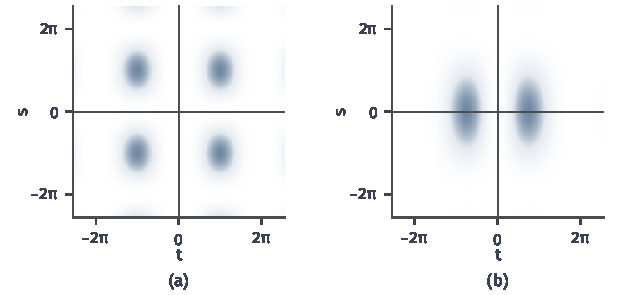
\includegraphics[width=108mm]{figures/07-probability/04-distribution-analysis/matplotlib/dep-cf-gap/figure.pdf}
  \caption{三点抛物线的特征函数之差。(a)$\lvert\Delta(t,s)\rvert^{2}=\frac{8}{81}(1-\cos t)^{2}(1-\cos s)$，白到蓝表示由小到大，在两条坐标轴上为零；(b)加权被积函数$\lvert\Delta\rvert^{2}/(\pi^{2}t^{2}s^{2})$，权重压低了高频，质量集中在$\lvert t\rvert\approx2$、$s$接近零的两块。(b)在全平面上的积分为$8/81$。}
  \label{fig:dep-cf-gap}
\end{BookInlineFigure}

\paragraph{权重不能随意替换}
零值判据的证明只用到权重处处为正与特征函数的唯一性；如果权重只在有界区域上为正，可能漏掉在那个区域外才出现的差别，因为两个不同的分布，其特征函数可以在一个区间上相同。权重的幂次也不能随意改动。若把$\lVert\bm{t}\rVert_2^{-(d+1)}$换成$\lVert\bm{t}\rVert_2^{-(d+\alpha)}$，引理的同样论证给出
\[
  \int_{\mathbb{R}^{d}}\frac{1-\cos\langle\bm{t},\bm{x}\rangle}{\lVert\bm{t}\rVert_2^{d+\alpha}}\,\mathrm{d}\bm{t}=c_{d,\alpha}\lVert\bm{x}\rVert_2^{\alpha},
\]
有限性要求原点附近$\lVert\bm{t}\rVert_2^{2-d-\alpha}$可积，即$\alpha<2$，无穷远处$\lVert\bm{t}\rVert_2^{-d-\alpha}$可积，即$\alpha>0$。所以$0<\alpha<2$时得到以$\lVert\bm{x}-\bm{x}'\rVert_2^{\alpha}$代替距离的一族度量，需要$\alpha$阶矩；$\alpha=2$时积分发散，下一小节会看到，强行把距离换成平方距离，零值判据就失效了。

\subsection{成对距离的表示}
\label{sec:dep-dcov-pairwise}

式~\eqref{eq:dep-dcov-def}是频率空间里的积分，实际计算时我们更希望回到取值空间。引理~\ref{lem:dep-cos-integral}已经把$1-\cos$换成距离，剩下的工作是把$\lvert\Delta\rvert^{2}$展开成若干个$1-\cos$的期望。为此引入$(\bm{X},\bm{Y})$的两个独立复制$(\bm{X}',\bm{Y}')$与$(\bm{X}'',\bm{Y}'')$，三组相互独立、同分布。

\begin{theorem}[距离协方差的成对距离表示]
\label{thm:dep-dcov-pairwise}
设$\mathbb{E}\lVert\bm{X}\rVert_2^{2}<\infty$，$\mathbb{E}\lVert\bm{Y}\rVert_2^{2}<\infty$。记$a=\lVert\bm{X}-\bm{X}'\rVert_2$，$b=\lVert\bm{Y}-\bm{Y}'\rVert_2$，$b''=\lVert\bm{Y}-\bm{Y}''\rVert_2$。则
\begin{equation}
  \operatorname{dCov}^{2}(\bm{X},\bm{Y})=\mathbb{E}[ab]+\mathbb{E}[a]\,\mathbb{E}[b]-2\,\mathbb{E}[ab''] .
  \label{eq:dep-dcov-pairwise}
\end{equation}
\end{theorem}

\begin{proof}
固定$(\bm{t},\bm{s})$，记三个随机相位
\[
  \theta=\langle\bm{t},\bm{X}-\bm{X}'\rangle,\qquad \eta=\langle\bm{s},\bm{Y}-\bm{Y}'\rangle,\qquad \eta''=\langle\bm{s},\bm{Y}-\bm{Y}''\rangle .
\]
用独立复制把$\lvert\Delta\rvert^{2}=\Delta\overline{\Delta}$的四项写成期望：
\[
  \begin{aligned}
    \phi_{\bm{X},\bm{Y}}\overline{\phi_{\bm{X},\bm{Y}}}&=\mathbb{E}\,\mathrm{e}^{\mathrm{i}(\theta+\eta)},\qquad
    \lvert\phi_{\bm{X}}\phi_{\bm{Y}}\rvert^{2}=\mathbb{E}\,\mathrm{e}^{\mathrm{i}\theta}\ \mathbb{E}\,\mathrm{e}^{\mathrm{i}\eta},\\
    \phi_{\bm{X},\bm{Y}}\overline{\phi_{\bm{X}}\phi_{\bm{Y}}}&=\mathbb{E}\,\mathrm{e}^{\mathrm{i}(\theta+\eta'')} .
  \end{aligned}
\]
第三项中$\overline{\phi_{\bm{X}}(\bm{t})}$用第二组复制写成期望，$\overline{\phi_{\bm{Y}}(\bm{s})}$用第三组复制。第四项是第三项的共轭。$\theta$与$-\theta$同分布，所以$\mathbb{E}\sin\theta=0$，同理$\mathbb{E}\sin\eta=0$。取实部，
\[
  \lvert\Delta\rvert^{2}=\mathbb{E}\cos\theta\cos\eta+\mathbb{E}\cos\theta\,\mathbb{E}\cos\eta-2\,\mathbb{E}\cos\theta\cos\eta''+S(\bm{t},\bm{s}),
\]
其中正弦部分为
\[
  S(\bm{t},\bm{s})=-\mathbb{E}\sin\theta\sin\eta+2\,\mathbb{E}\sin\theta\sin\eta'' .
\]

把$\cos\theta\cos\eta$写成$1-(1-\cos\theta)-(1-\cos\eta)+(1-\cos\theta)(1-\cos\eta)$，对另外两项同样展开。$\eta$与$\eta''$同分布，三项中常数与单个$1-\cos$的部分按系数$1+1-2=0$全部抵消。记$G(\bm{t},\bm{s})$为剩下的部分，
\[
  \begin{aligned}
  G={}&\mathbb{E}\bigl[(1-\cos\theta)(1-\cos\eta)\bigr]+\mathbb{E}[1-\cos\theta]\,\mathbb{E}[1-\cos\eta]\\
  &-2\,\mathbb{E}\bigl[(1-\cos\theta)(1-\cos\eta'')\bigr],
  \end{aligned}
\]
于是$\lvert\Delta\rvert^{2}=G+S$。

$S$关于$\bm{t}$是奇函数（$\bm{t}\to-\bm{t}$时$\sin\theta$变号），$G$是偶函数。权重关于$\bm{t}$对称，用代换$\bm{t}\to-\bm{t}$把式~\eqref{eq:dep-dcov-def}写成$\frac12(\lvert\Delta(\bm{t},\bm{s})\rvert^{2}+\lvert\Delta(-\bm{t},\bm{s})\rvert^{2})$的积分，这个平均正好是$G$。这一步只涉及非负函数的积分，不需要$S$可积。所以
\[
  \operatorname{dCov}^{2}(\bm{X},\bm{Y})=\frac{1}{c_pc_q}\int_{\mathbb{R}^{p+q}}\frac{G(\bm{t},\bm{s})}{\lVert\bm{t}\rVert_2^{p+1}\lVert\bm{s}\rVert_2^{q+1}}\,\mathrm{d}\bm{t}\,\mathrm{d}\bm{s}.
\]

$G$的三项各自是非负函数的期望。对第一项用Tonelli定理交换期望与积分，两次运用引理~\ref{lem:dep-cos-integral}，
\[
  \frac{1}{c_pc_q}\int\!\!\int\frac{\mathbb{E}[(1-\cos\theta)(1-\cos\eta)]}{\lVert\bm{t}\rVert_2^{p+1}\lVert\bm{s}\rVert_2^{q+1}}\,\mathrm{d}\bm{t}\,\mathrm{d}\bm{s}=\mathbb{E}[ab].
\]
第二、三项同理分别得到$\mathbb{E}[a]\mathbb{E}[b]$与$\mathbb{E}[ab'']$。由Cauchy--Schwarz不等式，$\mathbb{E}[ab]$不超过$(\mathbb{E}a^{2}\,\mathbb{E}b^{2})^{1/2}$，而由三角不等式$\mathbb{E}a^{2}$不超过$4\,\mathbb{E}\lVert\bm{X}\rVert_2^{2}$，是有限的，三项都有限，可以按线性逐项积分，得到式~\eqref{eq:dep-dcov-pairwise}。
\end{proof}

\paragraph{为什么需要二阶矩}
定义~\ref{def:dep-dcov}只需要一阶矩，式~\eqref{eq:dep-dcov-pairwise}却要求三项分别有限。只有一阶矩时，左边仍有限，右边可能是$\infty-\infty$。取$Y=X$，$X$服从第~\ref{chap:laws-of-large-numbers}章用过的$\alpha=1.5$的Pareto分布，$\mathbb{E}\lvert X\rvert<\infty$而$\mathbb{E}X^{2}=\infty$。这时$\mathbb{E}[ab]$就是$\mathbb{E}\lvert X-X'\rvert^{2}=\infty$，$\mathbb{E}[ab'']$也是无穷大，式~\eqref{eq:dep-dcov-pairwise}右边没有意义；而由式~\eqref{eq:dep-dcov-bound}，左边不超过$(\mathbb{E}\lvert X-X'\rvert)^{2}$，是有限的。二阶矩是让逐项展开合法的充分条件，不是距离协方差存在的条件。

\paragraph{双重中心化}
式~\eqref{eq:dep-dcov-pairwise}还可以写成一个“协方差”的样子。记$m(\bm{x})=\mathbb{E}\lVert\bm{x}-\bm{X}'\rVert_2$为点$\bm{x}$到$\bm{X}$的平均距离，$D=\mathbb{E}\lVert\bm{X}-\bm{X}'\rVert_2$。对成对距离作\term{双重中心化}（double centering），
\begin{equation}
  A(\bm{x},\bm{x}')=\lVert\bm{x}-\bm{x}'\rVert_2-m(\bm{x})-m(\bm{x}')+D ,
  \label{eq:dep-double-centering}
\end{equation}
即减去两端各自的平均距离，再加回总平均。对$\bm{Y}$同样定义$B(\bm{y},\bm{y}')$。则在定理~\ref{thm:dep-dcov-pairwise}的条件下
\begin{equation}
  \operatorname{dCov}^{2}(\bm{X},\bm{Y})=\mathbb{E}\bigl[A(\bm{X},\bm{X}')\,B(\bm{Y},\bm{Y}')\bigr].
  \label{eq:dep-dcov-centered}
\end{equation}

验证如下。记$n,D_Y$为$\bm{Y}$一侧与$m,D$对应的量。固定$\bm{y}$，对$\bm{Y}'$取期望，
\[
  \mathbb{E}\,B(\bm{y},\bm{Y}')=n(\bm{y})-n(\bm{y})-D_Y+D_Y=0 .
\]所以在$A$的四项中，只依赖$(\bm{X},\bm{Y})$一组的$m(\bm{X})$，与$B(\bm{Y},\bm{Y}')$相乘后先对$(\bm{X}',\bm{Y}')$取期望，得到零；$m(\bm{X}')$与常数$D$同理。只剩
\[
  \mathbb{E}\bigl[a\,B(\bm{Y},\bm{Y}')\bigr]=\mathbb{E}[ab]-\mathbb{E}\bigl[a\,n(\bm{Y})\bigr]-\mathbb{E}\bigl[a\,n(\bm{Y}')\bigr]+\mathbb{E}[a]\,D_Y .
\]
$n(\bm{Y})$是$b''$在给定$\bm{Y}$时的条件期望，所以$\mathbb{E}[a\,n(\bm{Y})]=\mathbb{E}[ab'']$；交换两组复制的角色，$\mathbb{E}[a\,n(\bm{Y}')]$也等于$\mathbb{E}[ab'']$。代回去就是式~\eqref{eq:dep-dcov-pairwise}的右边。

式~\eqref{eq:dep-dcov-centered}给出了一个直观的读法。$A(\bm{X},\bm{X}')>0$表示这一对$\bm{X}$比按各自位置预期的更远，$B>0$表示这一对$\bm{Y}$更远；距离协方差问的是“$\bm{X}$这对远时$\bm{Y}$这对是否也远”。中心化消去了只由一个边缘决定的部分：$m(\bm{x})$大只说明$\bm{x}$处在边缘分布的外围，与$\bm{Y}$无关。若$\bm{X},\bm{Y}$独立，则$(\bm{X},\bm{X}')$与$(\bm{Y},\bm{Y}')$独立，期望分解为$\mathbb{E}A\cdot\mathbb{E}B=0$。

\paragraph{平方距离只剩协方差}
现在可以看清为什么不能用平方距离。对实值变量把$\lvert x-x'\rvert$换成$(x-x')^{2}$，记$\mu=\mathbb{E}X$。$(x-x')^{2}$的平均是$m_2(x)=(x-\mu)^{2}+\operatorname{Var}(X)$，总平均是$2\operatorname{Var}(X)$，双重中心化后
\[
  (x-x')^{2}-m_2(x)-m_2(x')+2\operatorname{Var}(X)=-2(x-\mu)(x'-\mu).
\]
代入式~\eqref{eq:dep-dcov-centered}的形式，两组复制独立，
\[
  4\,\mathbb{E}\bigl[(X-\mu)(Y-\nu)(X'-\mu)(Y'-\nu)\bigr]=4\operatorname{Cov}(X,Y)^{2},
\]
其中$\nu=\mathbb{E}Y$。平方距离只保留了协方差，抛物线上为零；正是指数$1<2$使距离协方差看到了非线性的依赖。

\paragraph{三点抛物线的成对距离}
用式~\eqref{eq:dep-dcov-pairwise}重算三点抛物线。三个点的$x$坐标为$-1,0,1$，$y$坐标为$1,0,1$，成对距离矩阵为
\[
  \bm{A}=\begin{pmatrix}0&1&2\\1&0&1\\2&1&0\end{pmatrix},\qquad
  \bm{B}=\begin{pmatrix}0&1&0\\1&0&1\\0&1&0\end{pmatrix}.
\]
三点等可能，期望就是对$9$个元素求平均。第一项$\mathbb{E}[ab]$只在$\bm{B}$非零的四个位置有贡献，那里$\bm{A}$的元素都是$1$，
\[
  \mathbb{E}[ab]=\tfrac49,\qquad \mathbb{E}[a]=\tfrac89,\qquad \mathbb{E}[b]=\tfrac49 .
\]

第三项要先求每个点的平均距离：$\bm{A}$的行平均是$m=(1,\frac23,1)$，$\bm{B}$的行平均是$n=(\frac13,\frac23,\frac13)$。由$\mathbb{E}[ab'']=\mathbb{E}[m(X)\,n(Y)]$，
\[
  \mathbb{E}[ab'']=\tfrac13\Bigl(1\cdot\tfrac13+\tfrac23\cdot\tfrac23+1\cdot\tfrac13\Bigr)=\tfrac{10}{27}.
\]
代入式~\eqref{eq:dep-dcov-pairwise}，
\[
  \operatorname{dCov}^{2}(X,Y)=\frac49+\frac89\cdot\frac49-2\cdot\frac{10}{27}=\frac{36+32-60}{81}=\frac{8}{81},
\]
与特征函数积分的结果一致。

图~\ref{fig:dep-double-centering}给出双重中心化后的矩阵$\tilde{\bm{A}}$、$\tilde{\bm{B}}$：每行每列之和为零。按式~\eqref{eq:dep-dcov-centered}逐格相乘求和，
\[
  \frac19\sum_{i,j}\tilde{A}_{i,j}\tilde{B}_{i,j}=\frac19\cdot\frac{72}{81}=\frac{8}{81}.
\]

\begin{BookInlineFigure}
  \centering
  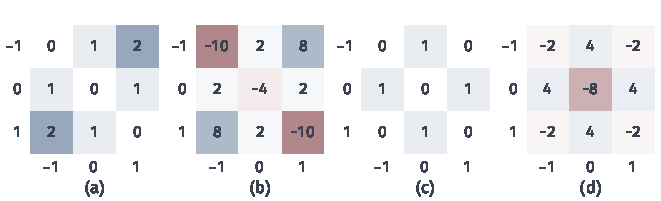
\includegraphics[width=112mm]{figures/07-probability/04-distribution-analysis/matplotlib/dep-double-centering/figure.pdf}
  \caption{三点抛物线的成对距离与双重中心化，行列按$x=-1,0,1$排列。(a)$\bm{A}=(\lvert x_i-x_j\rvert)$；(b)$\tilde{\bm{A}}$，格中数字乘以$1/9$；(c)$\bm{B}=(\lvert y_i-y_j\rvert)$；(d)$\tilde{\bm{B}}$，格中数字乘以$1/9$。(a)(c)白到蓝表示由小到大，(b)(d)红—白—蓝表示由负到正。中心化后每行每列之和为零。}
  \label{fig:dep-double-centering}
\end{BookInlineFigure}

$n$个样本点的经验分布也是这样一个等可能的有限分布，把式~\eqref{eq:dep-dcov-pairwise}用在经验分布上，就得到样本距离协方差。它作为总体量估计的性质，属于统计推断的问题。

\subsection{距离相关}
\label{sec:dep-dcor}

距离协方差有量纲：把$\bm{Y}$的单位从米换成厘米，$\operatorname{dCov}^{2}$乘以$100$。与由协方差得到相关系数一样，用各自的“距离方差”归一化。

\begin{definition}[距离相关]
\label{def:dep-dcor}
在定义~\ref{def:dep-dcov}的条件下，称$\bm{X}$与自身的距离协方差$\operatorname{dCov}^{2}(\bm{X},\bm{X})$为$\bm{X}$的\term{距离方差}（distance variance），记为$\operatorname{dVar}^{2}(\bm{X})$。$\bm{X}$与$\bm{Y}$的\term{距离相关}（distance correlation）定义为
\begin{equation}
  \operatorname{dCor}(\bm{X},\bm{Y})=
  \begin{cases}
    \dfrac{\operatorname{dCov}(\bm{X},\bm{Y})}{\sqrt{\operatorname{dVar}(\bm{X})\operatorname{dVar}(\bm{Y})}}, & \operatorname{dVar}(\bm{X})\operatorname{dVar}(\bm{Y})>0,\\
    0, & \operatorname{dVar}(\bm{X})\operatorname{dVar}(\bm{Y})=0 .
  \end{cases}
  \label{eq:dep-dcor}
\end{equation}
\end{definition}

第二行的约定只在常量情形起作用。由定理~\ref{thm:dep-dcov-independence}，$\operatorname{dVar}^{2}(\bm{X})=0$当且仅当$\bm{X}$与自身独立；这时对每个Borel集$C$，事件$\{\bm{X}\in C\}$与自身独立，它的概率$r$满足$r=r^{2}$，只能是$0$或$1$，每个坐标的分布函数只取$0,1$两个值，$\bm{X}$几乎必然是常数。常数与任何变量都独立，取距离相关为$0$与零值判据相容。

\begin{theorem}[距离相关的范围与不变性]
\label{thm:dep-dcor-properties}
在定义~\ref{def:dep-dcor}的条件下：
\begin{enumerate}
  \item $0\leq\operatorname{dCor}(\bm{X},\bm{Y})\leq1$，并且$\operatorname{dCor}(\bm{X},\bm{Y})=0$当且仅当$\bm{X}$与$\bm{Y}$独立；
  \item 对向量$\bm{a}_1\in\mathbb{R}^{p}$、$\bm{a}_2\in\mathbb{R}^{q}$，非零标量$b_1,b_2$与正交矩阵$\bm{C}_1,\bm{C}_2$，
  \begin{equation}
    \operatorname{dCov}^{2}(\bm{a}_1+b_1\bm{C}_1\bm{X},\ \bm{a}_2+b_2\bm{C}_2\bm{Y})=\lvert b_1b_2\rvert\operatorname{dCov}^{2}(\bm{X},\bm{Y}),
    \label{eq:dep-dcov-scaling}
  \end{equation}
  从而距离相关在这类变换下不变。
\end{enumerate}
\end{theorem}

\begin{proof}
零值部分由定理~\ref{thm:dep-dcov-independence}与常量约定直接得到。上界先在二阶矩有限时证明。由式~\eqref{eq:dep-dcov-centered}与Cauchy--Schwarz不等式，
\[
  \operatorname{dCov}^{2}(\bm{X},\bm{Y})\leq\bigl(\mathbb{E}A^{2}\bigr)^{1/2}\bigl(\mathbb{E}B^{2}\bigr)^{1/2}=\operatorname{dVar}(\bm{X})\operatorname{dVar}(\bm{Y}),
\]
最后一步对$\bm{Y}=\bm{X}$与$\bm{X}=\bm{Y}$再用一次式~\eqref{eq:dep-dcov-centered}。两边开方，除以$\operatorname{dVar}(\bm{X})\operatorname{dVar}(\bm{Y})$，得$\operatorname{dCor}\leq1$。

对第二部分，记$\bm{X}^{*}=\bm{a}_1+b_1\bm{C}_1\bm{X}$，它的特征函数为
\[
  \phi_{\bm{X}^{*}}(\bm{t})=\mathrm{e}^{\mathrm{i}\langle\bm{t},\bm{a}_1\rangle}\phi_{\bm{X}}\bigl(b_1\bm{C}_1^{\top}\bm{t}\bigr),
\]
联合特征函数同理。平移因子的模为$1$，所以变换后的差$\Delta^{*}$满足
\[
  \lvert\Delta^{*}(\bm{t},\bm{s})\rvert=\bigl\lvert\Delta\bigl(b_1\bm{C}_1^{\top}\bm{t},\,b_2\bm{C}_2^{\top}\bm{s}\bigr)\bigr\rvert .
\]
在式~\eqref{eq:dep-dcov-def}中作代换$\bm{u}=b_1\bm{C}_1^{\top}\bm{t}$。体积元变为$\lvert b_1\rvert^{-p}\mathrm{d}\bm{u}$，分母变为$\lvert b_1\rvert^{-p-1}\lVert\bm{u}\rVert_2^{p+1}$，积分多出因子$\lvert b_1\rvert$。$\bm{s}$一侧同样多出$\lvert b_2\rvert$，这就是式~\eqref{eq:dep-dcov-scaling}。对$\operatorname{dVar}^{2}$分别多出$b_1^{2}$与$b_2^{2}$，代入式~\eqref{eq:dep-dcor}相消。
\end{proof}

上界的证明用到了二阶矩。只有一阶矩时上界同样成立，需要先截断再验证各项的连续性，篇幅较长，可查阅\scite{math-szekely2007dependence}。

距离相关取到$1$的情形也已清楚：$\operatorname{dCor}(\bm{X},\bm{Y})=1$当且仅当$\bm{Y}=\bm{a}+b\bm{C}\bm{X}$几乎必然成立，其中$b\neq0$为标量、$\bm{C}$为正交矩阵，证明见同一文献。所以距离相关为$1$意味着两组坐标只差一个相似变换，比“$\bm{Y}$由$\bm{X}$确定”严格得多。

\paragraph{三点抛物线与高斯}
三点抛物线的距离方差由图~\ref{fig:dep-double-centering}的矩阵算出。中心化一侧即可，
\[
  \operatorname{dVar}^{2}(X)=\frac19\sum_{i,j}\tilde{A}_{i,j}A_{i,j}=\frac{40}{81},\qquad \operatorname{dVar}^{2}(Y)=\frac19\sum_{i,j}\tilde{B}_{i,j}B_{i,j}=\frac{16}{81}.
\]代入式~\eqref{eq:dep-dcor}，
\[
  \operatorname{dCor}^{2}(X,Y)=\frac{8/81}{\sqrt{(40/81)(16/81)}}=\frac{8}{\sqrt{640}}=\frac{1}{\sqrt{10}},
\]
所以$\operatorname{dCor}(X,Y)=10^{-1/4}\approx0.562$。$Y$由$X$确定，距离相关却远小于$1$，因为$Y=X^{2}$不是$X$的相似变换。

同一文献还算出了标准二元高斯的闭式结果：
\[
  \operatorname{dCor}^{2}=\frac{\rho\arcsin\rho+\sqrt{1-\rho^{2}}-\rho\arcsin(\rho/2)-\sqrt{4-\rho^{2}}+1}{1+\pi/3-\sqrt3}.
\]
$\rho=0.5$时约为$0.206$，即$\operatorname{dCor}\approx0.454$。图~\ref{fig:dep-dcor-gaussian}显示距离相关在高斯族内随$\lvert\rho\rvert$单调增，略低于$\lvert\rho\rvert$，两端与之重合。在高斯族内两者给出相同的次序，只是刻度不同。

\begin{BookInlineFigure}
  \centering
  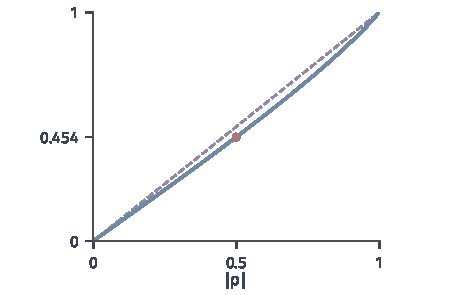
\includegraphics[width=80mm]{figures/07-probability/04-distribution-analysis/matplotlib/dep-dcor-gaussian/figure.pdf}
  \caption{标准二元高斯的距离相关随$\lvert\rho\rvert$的变化（蓝，闭式公式；脚本另用$60\times60$个Gauss--Hermite节点数值核对，相对误差在$0.3\%$以内）。紫色虚线是参考线$\lvert\rho\rvert$。红点为$\rho=0.5$处的$0.454$。}
  \label{fig:dep-dcor-gaussian}
\end{BookInlineFigure}

\paragraph{哪些变换保持距离相关}
定理~\ref{thm:dep-dcor-properties}允许的变换是平移、旋转（含反射）与同一个非零标量的整体缩放，它们保持距离之间的比例。其他变换一般会改变距离相关。把三点抛物线中$X$的取值$-1,0,1$改成$-1,0,5$，互信息不变，距离相关从$0.562$变为$0.530$。对高斯向量作坐标变换$(\mathrm{e}^{X},\mathrm{e}^{Y})$，距离相关从$0.454$变为约$0.42$；用$\Phi$变到Copula坐标，约为$0.45$；把$Y$整体乘以$10$则不变。图~\ref{fig:dep-transform-bars}把相关系数、距离相关与互信息放在一起比较：互信息在四种变换下都不动，距离相关只在相似变换下不动。若对$\bm{X}$的不同坐标用不同的比例缩放，例如$\operatorname{diag}(1,10)$，距离的比例被打乱，距离相关一般也会改变；多维时先统一各坐标的单位，再计算距离相关。

\begin{BookInlineFigure}
  \centering
  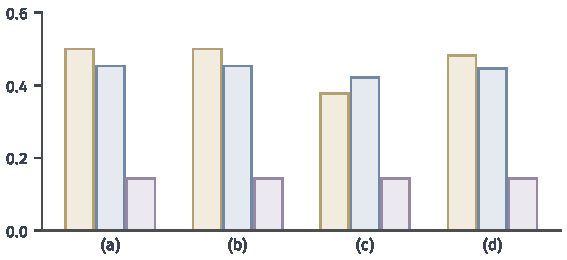
\includegraphics[width=96mm]{figures/07-probability/04-distribution-analysis/matplotlib/dep-transform-bars/figure.pdf}
  \caption{标准二元高斯（$\rho=0.5$）在四种坐标变换下的三个量：(a)原坐标；(b)$Y\mapsto10Y$；(c)$(\mathrm{e}^{X},\mathrm{e}^{Y})$；(d)$(\Phi(X),\Phi(Y))$。黄柱为相关系数的绝对值，蓝柱为距离相关（$90\times90$个Gauss--Hermite加权节点数值计算，约$0.453$、$0.453$、$0.422$、$0.445$），紫柱为互信息（nat，均为$0.144$）。}
  \label{fig:dep-transform-bars}
\end{BookInlineFigure}


\section{HSIC}
\label{sec:dep-hsic}

距离协方差用一种特定的权重比较特征函数，并且只适用于欧氏空间。第~\ref{chap:distribution-comparison}章的MMD给了比较两个分布的另一种通用办法：把分布映成再生核Hilbert空间中的核均值，再量两个核均值的距离。独立性问的正是两个分布$P_{(X,Y)}$与$P_X\otimes P_Y$是否相同，只要在乘积空间上选一个核，就能直接用MMD比较它们。

先回顾所用的记号。$k$是$\mathcal{X}$上的正定核，$\mathcal{H}_k$是它的RKHS。对满足$\mathbb{E}_{P}\sqrt{k(X,X)}<\infty$的分布$P$，核均值$m_P\in\mathcal{H}_k$由
\[
  \mathbb{E}_{P}[g(X)]=\langle g,m_P\rangle_{\mathcal{H}_k},\qquad g\in\mathcal{H}_k
\]
确定，取值为$m_P(y)=\mathbb{E}_{P}[k(X,y)]$。两个分布的MMD是两个核均值之差的范数$\lVert m_P-m_Q\rVert_{\mathcal{H}_k}$，记为$\operatorname{MMD}_k(P,Q)$，它等于$\mathcal{H}_k$单位球上期望差的最大值，平方可以写成核期望
\begin{equation}
  \operatorname{MMD}_k^{2}(P,Q)=\mathbb{E}\,k(U,U')-2\,\mathbb{E}\,k(U,V)+\mathbb{E}\,k(V,V'),
  \label{eq:dep-mmd-recall}
\end{equation}
其中$U,U'\sim P$，$V,V'\sim Q$，四者相互独立。若$P\mapsto m_P$是单射，称$k$为特征核，这时MMD为零当且仅当两个分布相同；欧氏空间上固定带宽的高斯核是特征核。

\subsection{联合分布的核比较}
\label{sec:dep-hsic-kernel-comparison}

在$\mathcal{X}$上取核$k$，在$\mathcal{Y}$上取核$l$。乘积空间$\mathcal{X}\times\mathcal{Y}$上最自然的核是两者的乘积
\[
  \kappa\bigl((x,y),(x',y')\bigr)=k(x,x')\,l(y,y'),
\]
称为\term{乘积核}（product kernel）。它仍是正定核：其Gram矩阵是两个Gram矩阵的逐元素乘积，正定性由Schur乘积定理保证，可参考\BookChapterRef{chap:rkhs}{卷四第23章“再生核Hilbert空间”}。本节假定$k,l$可测且有界，相应的RKHS可分，于是$\kappa$也有界，任何分布的核均值都存在。

\begin{definition}[HSIC]
\label{def:dep-hsic}
在上述条件下，$X$与$Y$关于核$k,l$的\term{Hilbert--Schmidt独立性准则}（Hilbert--Schmidt independence criterion），简称HSIC，定义为
\begin{equation}
  \operatorname{HSIC}_{k,l}(X,Y)=\operatorname{MMD}_{\kappa}^{2}\bigl(P_{(X,Y)},\,P_X\otimes P_Y\bigr).
  \label{eq:dep-hsic-def}
\end{equation}
\end{definition}

图~\ref{fig:dep-hsic-embedding}是这个定义的示意：两个分布各被送到$\mathcal{H}_\kappa$中的一个点，HSIC是这两点距离的平方。边缘乘积的核均值是$m_{P_X}$与$m_{P_Y}$的张量积：对独立的$\tilde{X}\sim P_X$、$\tilde{Y}\sim P_Y$，期望分解为
\[
  \mathbb{E}\bigl[k(\tilde{X},x)\,l(\tilde{Y},y)\bigr]=m_{P_X}(x)\,m_{P_Y}(y).
\]

\begin{BookInlineFigure}
  \centering
  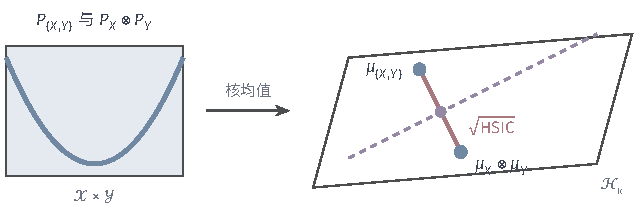
\includegraphics[width=107.9mm]{figures/07-probability/04-distribution-analysis/tikz/dep-hsic-embedding/figure.pdf}
  \caption{HSIC的几何图景。左：乘积空间上的两个分布，联合分布的质量集中在蓝色曲线上，边缘乘积摊在整个浅蓝矩形上。右：乘积核的RKHS$\mathcal{H}_\kappa$，两个核均值是两个蓝点，红色线段长度是$\sqrt{\operatorname{HSIC}}$。紫色虚线示意一个较贫乏的核只能看到的子空间：两个点在其上的投影（紫点）重合，这样的核给出零值。}
  \label{fig:dep-hsic-embedding}
\end{BookInlineFigure}

把式~\eqref{eq:dep-mmd-recall}用到这两个分布上，就得到只含核期望的表达。

\begin{theorem}[HSIC的核期望表示]
\label{thm:dep-hsic-expectation}
设$(X,Y)$、$(X',Y')$、$(X'',Y'')$相互独立且同分布。则
\begin{equation}
  \begin{aligned}
  \operatorname{HSIC}_{k,l}(X,Y)={}&\mathbb{E}\bigl[k(X,X')\,l(Y,Y')\bigr]+\mathbb{E}\bigl[k(X,X')\bigr]\,\mathbb{E}\bigl[l(Y,Y')\bigr]\\
  &-2\,\mathbb{E}\bigl[k(X,X')\,l(Y,Y'')\bigr].
  \end{aligned}
  \label{eq:dep-hsic-expectation}
\end{equation}
\end{theorem}

\begin{proof}
在式~\eqref{eq:dep-mmd-recall}中取$P=P_{(X,Y)}$，$Q=P_X\otimes P_Y$。第一项取$U=(X,Y)$，$U'=(X',Y')$，得$\mathbb{E}[k(X,X')l(Y,Y')]$。第三项中$V,V'$都服从边缘乘积，可以取$V=(X,Y'')$、$V'=(X',Y''')$，其中$Y'''$来自第四组独立复制；四个分量相互独立，期望分解为$\mathbb{E}[k(X,X')]\,\mathbb{E}[l(Y,Y')]$。第二项中$U=(X,Y)$，$V$服从边缘乘积且与$U$独立，取$V=(X',Y'')$，得到$\mathbb{E}[k(X,X')l(Y,Y'')]$。核有界，所有期望有限，代入即得。
\end{proof}

式~\eqref{eq:dep-hsic-expectation}与距离协方差的式~\eqref{eq:dep-dcov-pairwise}结构完全相同，只是把成对距离换成了核值。距离量的是“不相似”，核量的是“相似”，两者都在问：$X$这一对相似时，$Y$这一对是否也相似，超出边缘分布本身所能解释的程度。

\paragraph{中心化核}
与双重中心化同样，令
\[
  \tilde{k}(x,x')=k(x,x')-m_{P_X}(x)-m_{P_X}(x')+\mathbb{E}\,k(X,X'),
\]
称为\term{中心化核}（centered kernel），$\tilde{l}$类似。重复式~\eqref{eq:dep-dcov-centered}的验证（那里只用到中心化后对单个复制取期望为零），得到
\begin{equation}
  \operatorname{HSIC}_{k,l}(X,Y)=\mathbb{E}\bigl[\tilde{k}(X,X')\,\tilde{l}(Y,Y')\bigr].
  \label{eq:dep-hsic-centered}
\end{equation}
由再生性质展开可知，$\tilde{k}(x,x')$等于$k(x,\cdot)-m_{P_X}$与$k(x',\cdot)-m_{P_X}$在$\mathcal{H}_k$中的内积，就是把特征点平移到以核均值为原点后的内积。

\paragraph{交叉协方差算子}
HSIC这个名字来自另一种写法。对$f\in\mathcal{H}_k$、$g\in\mathcal{H}_l$，考虑$f(X)$与$g(Y)$的协方差。它对$f$、$g$都是线性的。由再生性质，$\lvert f(x)\rvert$不超过$\lVert f\rVert_{\mathcal{H}_k}\sqrt{k(x,x)}$，核有界时协方差被常数倍的$\lVert f\rVert\,\lVert g\rVert$控制。由Riesz表示定理，存在有界线性算子$\mathcal{C}_{XY}:\mathcal{H}_l\to\mathcal{H}_k$，使
\[
  \langle f,\mathcal{C}_{XY}\,g\rangle_{\mathcal{H}_k}=\operatorname{Cov}\bigl(f(X),g(Y)\bigr),
\]
称为\term{交叉协方差算子}（cross-covariance operator）。取$\mathcal{H}_k$与$\mathcal{H}_l$的规范正交基$\{e_i\}$、$\{e'_j\}$，HSIC等于这个算子的Hilbert--Schmidt范数的平方，
\begin{equation}
  \operatorname{HSIC}_{k,l}(X,Y)=\sum_{i,j}\operatorname{Cov}\bigl(e_i(X),\,e'_j(Y)\bigr)^{2}.
  \label{eq:dep-hsic-operator}
\end{equation}

式~\eqref{eq:dep-hsic-operator}可以从式~\eqref{eq:dep-hsic-centered}推出。记$\tilde{e}_i(x)=e_i(x)-\mathbb{E}e_i(X)$，由再生性质它等于$e_i$与$k(x,\cdot)-m_{P_X}$的内积。由Parseval等式，
\[
  \sum_i\tilde{e}_i(x)\,\tilde{e}_i(x')=\bigl\langle k(x,\cdot)-m_{P_X},\,k(x',\cdot)-m_{P_X}\bigr\rangle=\tilde{k}(x,x'),
\]
$\tilde{l}$同样展开。部分和由Cauchy--Schwarz不等式被$\lVert k(x,\cdot)-m_{P_X}\rVert\lVert k(x',\cdot)-m_{P_X}\rVert$控制，核有界时这是常数，可以用支配收敛定理交换求和与期望：
\[
  \mathbb{E}\bigl[\tilde{k}(X,X')\tilde{l}(Y,Y')\bigr]=\sum_{i,j}\mathbb{E}\bigl[\tilde{e}_i(X)\tilde{e}'_j(Y)\bigr]\,\mathbb{E}\bigl[\tilde{e}_i(X')\tilde{e}'_j(Y')\bigr].
\]
两组复制独立，每个乘积因子都是$\operatorname{Cov}(e_i(X),e'_j(Y))$，即得式~\eqref{eq:dep-hsic-operator}。

这个写法给出了直观：HSIC同时检查无穷多对特征函数$e_i(X)$、$e'_j(Y)$之间的协方差，把它们的平方加起来。协方差只检查一对线性函数；核越丰富，被检查的函数对越多。

\paragraph{线性核只剩协方差}
取最贫乏的核，$\mathcal{X}=\mathcal{Y}=\mathbb{R}$上的线性核$k(x,x')=xx'$、$l(y,y')=yy'$。它们无界，但当$X,Y$有二阶矩时式~\eqref{eq:dep-hsic-expectation}的各项仍然有限。代入，
\[
  \begin{aligned}
  &\mathbb{E}[XX'YY']+\mathbb{E}[XX']\,\mathbb{E}[YY']-2\,\mathbb{E}[XX'YY'']\\
  &\qquad=(\mathbb{E}XY)^{2}+(\mathbb{E}X)^{2}(\mathbb{E}Y)^{2}-2\,\mathbb{E}XY\,\mathbb{E}X\,\mathbb{E}Y ,
  \end{aligned}
\]
右边正是$\operatorname{Cov}(X,Y)^{2}$。线性核的RKHS只含线性函数，式~\eqref{eq:dep-hsic-operator}只剩一项。三点抛物线和连续抛物线在线性核下HSIC都是零。

\paragraph{距离诱导核}
距离协方差也是一个HSIC，只是用的核无界。在$\mathbb{R}^{d}$上令
\[
  k_{\mathrm{d}}(\bm{x},\bm{x}')=\tfrac12\bigl(\lVert\bm{x}\rVert_2+\lVert\bm{x}'\rVert_2-\lVert\bm{x}-\bm{x}'\rVert_2\bigr),
\]
称为\term{距离诱导核}（distance-induced kernel）。

它是正定的。由引理~\ref{lem:dep-cos-integral}，$k_{\mathrm{d}}$的三项各写成$1-\cos$的积分。记$\alpha=\langle\bm{t},\bm{x}\rangle$，$\beta=\langle\bm{t},\bm{x}'\rangle$，展开右边的乘积可以验证
\[
  \begin{aligned}
  &(1-\cos\alpha)+(1-\cos\beta)-\bigl(1-\cos(\alpha-\beta)\bigr)\\
  &\qquad=\operatorname{Re}\bigl[(\mathrm{e}^{\mathrm{i}\alpha}-1)\,\overline{(\mathrm{e}^{\mathrm{i}\beta}-1)}\bigr].
  \end{aligned}
\]
记
\[
  g_{\bm{x}}(\bm{t})=\mathrm{e}^{\mathrm{i}\langle\bm{t},\bm{x}\rangle}-1 .
\]

把三项的积分合并，得到
\[
  k_{\mathrm{d}}(\bm{x},\bm{x}')=\frac{1}{2c_d}\int_{\mathbb{R}^{d}}\frac{\operatorname{Re}\bigl[g_{\bm{x}}(\bm{t})\overline{g_{\bm{x}'}(\bm{t})}\bigr]}{\lVert\bm{t}\rVert_2^{d+1}}\,\mathrm{d}\bm{t},
\]
这是一个加权$L^{2}$内积的实部。对任意点$\bm{x}_1,\dots,\bm{x}_n$与实数$c_1,\dots,c_n$，
\[
  \sum_{i,j}c_ic_j\,k_{\mathrm{d}}(\bm{x}_i,\bm{x}_j)=\frac{1}{2c_d}\int_{\mathbb{R}^{d}}\frac{\bigl\lvert\sum_ic_ig_{\bm{x}_i}(\bm{t})\bigr\rvert^{2}}{\lVert\bm{t}\rVert_2^{d+1}}\,\mathrm{d}\bm{t}\geq0 .
\]

$k_{\mathrm{d}}$中的$\lVert\bm{x}\rVert_2$与$\lVert\bm{x}'\rVert_2$只依赖一个端点，在中心化中被消去，所以$\tilde{k}_{\mathrm{d}}=-\frac12A$，$A$是式~\eqref{eq:dep-double-centering}的双重中心化距离。代入式~\eqref{eq:dep-hsic-centered}与式~\eqref{eq:dep-dcov-centered}，在二阶矩有限时
\[
  \operatorname{HSIC}_{k_{\mathrm{d}},l_{\mathrm{d}}}(\bm{X},\bm{Y})=\tfrac14\operatorname{dCov}^{2}(\bm{X},\bm{Y}).
\]
距离协方差因此是HSIC的一个特例。核无界时，HSIC的每一项能否积分要另外检查，这里所需的正是二阶矩。

\paragraph{两个手算例子}
标准二元高斯在高斯核下有闭式。取$k(x,x')=\exp(-(x-x')^{2}/2)$，$l$相同（带宽$1$）。式~\eqref{eq:dep-hsic-expectation}的每一项都形如$\mathbb{E}\exp(-\frac12(U^{2}+V^{2}))$，其中$(U,V)$是均值为零的二元高斯，协方差矩阵记为$\bm{S}$。把高斯密度代入并配方，
\[
  \mathbb{E}\exp\Bigl(-\tfrac12(U^{2}+V^{2})\Bigr)=\frac{1}{2\pi\sqrt{\det\bm{S}}}\int_{\mathbb{R}^{2}}\mathrm{e}^{-\frac12\bm{w}^{\top}(\bm{S}^{-1}+\bm{I})\bm{w}}\,\mathrm{d}\bm{w}=\det(\bm{I}+\bm{S})^{-1/2}.
\]
三项分别对应$(U,V)=(X-X',Y-Y')$、两者独立、$(X-X',Y-Y'')$，协方差矩阵的对角元都是$2$，非对角元分别为$2\rho$、$0$、$\rho$。$\det(\bm{I}+\bm{S})$依次为$9-4\rho^{2}$、$9$、$9-\rho^{2}$，于是
\begin{equation}
  \operatorname{HSIC}=\frac{1}{\sqrt{9-4\rho^{2}}}+\frac13-\frac{2}{\sqrt{9-\rho^{2}}}.
  \label{eq:dep-hsic-gauss}
\end{equation}
$\rho=0.5$时三项为$0.35355$、$0.33333$、$-0.67612$，
\[
  \operatorname{HSIC}\approx0.35355+0.33333-0.67612=0.01076 .
\]

三点抛物线在同样的核下是有限和。记$\alpha=\mathrm{e}^{-1/2}\approx0.6065$，$\beta=\mathrm{e}^{-2}\approx0.1353$，三个点按$x=-1,0,1$排列，核矩阵为
\[
  \bm{K}=\begin{pmatrix}1&\alpha&\beta\\ \alpha&1&\alpha\\ \beta&\alpha&1\end{pmatrix},\qquad
  \bm{L}=\begin{pmatrix}1&\alpha&1\\ \alpha&1&\alpha\\ 1&\alpha&1\end{pmatrix}.
\]
式~\eqref{eq:dep-hsic-expectation}的三项分别是$\frac19\sum_{i,j}K_{i,j}L_{i,j}$、两个矩阵各自的元素平均之积、以及$\frac13\sum_i\bar{K}_i\bar{L}_i$（$\bar{K}_i,\bar{L}_i$为第$i$行的平均）。数值为
\[
  \begin{gathered}
  \mathbb{E}[kl]\approx0.52691,\qquad \mathbb{E}[kl'']\approx0.51771,\\
  \mathbb{E}[k]\,\mathbb{E}[l]\approx0.63298\times0.82512\approx0.52228,
  \end{gathered}
\]
所以$\operatorname{HSIC}\approx0.52691+0.52228-2\times0.51771\approx0.01378$。

\subsection{零值判据与核选择}
\label{sec:dep-hsic-zero}

由定义~\ref{def:dep-hsic}，HSIC为零当且仅当两个核均值相同。核均值能否分辨$P_{(X,Y)}$与$P_X\otimes P_Y$，取决于乘积核$\kappa$。

\begin{theorem}[HSIC的零值判据]
\label{thm:dep-hsic-zero}
若乘积核$\kappa=k\otimes l$在$\mathcal{X}\times\mathcal{Y}$的概率分布上是特征核，则
\begin{equation}
  \operatorname{HSIC}_{k,l}(X,Y)=0\iff X\text{与}Y\text{独立}.
  \label{eq:dep-hsic-zero}
\end{equation}
特别地，$\mathcal{X}=\mathbb{R}^{p}$、$\mathcal{Y}=\mathbb{R}^{q}$，$k,l$为带宽$\sigma,\tau>0$的高斯核时，结论成立。
\end{theorem}

\begin{proof}
式~\eqref{eq:dep-hsic-zero}是特征核的定义：MMD为零当且仅当两个分布相同。对高斯核，乘积核为
\[
  \kappa\bigl((\bm{x},\bm{y}),(\bm{x}',\bm{y}')\bigr)=\exp\Bigl(-\frac{\lVert\bm{x}-\bm{x}'\rVert_2^{2}}{2\sigma^{2}}-\frac{\lVert\bm{y}-\bm{y}'\rVert_2^{2}}{2\tau^{2}}\Bigr).
\]
作线性变换$T(\bm{x},\bm{y})=(\bm{x}/\sigma,\bm{y}/\tau)$，则$\kappa(\bm{z},\bm{z}')=k_1(T\bm{z},T\bm{z}')$，$k_1$是$\mathbb{R}^{p+q}$上带宽为$1$的高斯核。若两个分布$P,Q$的$\kappa$核均值相同，则推前分布$T_{\#}P$与$T_{\#}Q$的$k_1$核均值相同；$k_1$是特征核，所以$T_{\#}P=T_{\#}Q$，$T$可逆，于是$P=Q$。
\end{proof}

若$\sigma=\tau$，把第~\ref{chap:distribution-comparison}章高斯核MMD的谱表示用到$\mathbb{R}^{p+q}$上，HSIC就是$\lvert\Delta(\bm{t},\bm{s})\rvert^{2}$对高斯分布$\mathcal{N}(\bm{0},\sigma^{-2}\bm{I})$的积分。它与距离协方差的定义~\eqref{eq:dep-dcov-def}只差权重：高斯权重是可积的概率密度，不需要矩条件，但强烈压低高频；距离协方差的幂次权重不可积，换来了与距离的对应和尺度上的等变性。

特征核是充分条件。对欧氏空间上的平移不变核，已知只要$k$与$l$各自是特征核，HSIC的零值就刻画独立\scite{math-gretton2015hsic}。核不够丰富时，HSIC为零只说明它所检查的那些函数对的协方差都为零，例如线性核下只说明不相关。图~\ref{fig:dep-hsic-embedding}中紫色虚线表示的正是这种情况。

\paragraph{核尺度改变数值}
高斯核的带宽决定了HSIC“在多大尺度上看”。带宽很小时，核只在几乎重合的点对上取值接近$1$，连续分布下各项都趋于零；带宽很大时，在数据范围内$k(x,x')\approx1-(x-x')^{2}/(2\sigma^{2})$，核近似退化为常数加二次项，HSIC按$\sigma^{-4}$趋于零，并且主要反映协方差。中间某个尺度上HSIC最大。

图~\ref{fig:dep-hsic-bandwidth}对比两个分布：$\rho=0.5$的标准二元高斯（式~\eqref{eq:dep-hsic-gauss}的推广）与连续抛物线（数值积分），两个坐标用相同带宽$s$。抛物线的取值范围小，在$s\approx0.19$处达到最大值约$0.067$；高斯在$s\approx0.95$处达到约$0.0108$。两条曲线在$s\approx0.7$与$0.78$之间相交：带宽小于此时抛物线的HSIC更大，大于此时高斯的更大。$s=1$时两者分别为$0.0108$与$0.0026$。

\begin{BookInlineFigure}
  \centering
  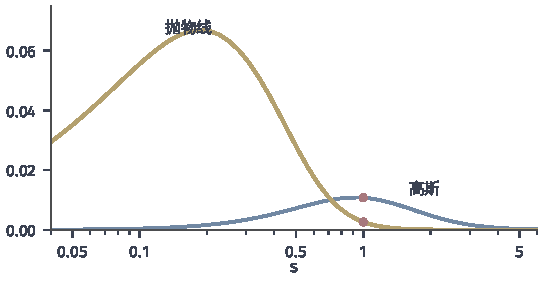
\includegraphics[width=92mm]{figures/07-probability/04-distribution-analysis/matplotlib/dep-hsic-bandwidth/figure.pdf}
  \caption{高斯核HSIC随带宽$s$的变化（横轴为对数刻度，两个坐标用同一带宽）。蓝线：$\rho=0.5$的标准二元高斯，闭式计算；黄线：$X\sim\operatorname{Unif}(-1,1)$、$Y=X^{2}$，对$X$取$1000$个节点数值积分。红点为$s=1$处的$0.0108$与$0.0026$。两条曲线在$s\approx0.74$附近相交。}
  \label{fig:dep-hsic-bandwidth}
\end{BookInlineFigure}

所以“这个分布的HSIC比那个大”只有在指定了核与带宽以后才有意义；换一个带宽，次序可以颠倒。不同核下的HSIC数值不在同一个刻度上，不能直接比较。把HSIC除以$\sqrt{\operatorname{HSIC}_{k,k}(X,X)\operatorname{HSIC}_{l,l}(Y,Y)}$可以得到与距离相关类似的归一化量，它消去了一部分尺度影响，但仍依赖带宽。根据样本选带宽的经验规则涉及估计问题，不在本章讨论。


\section{离散化评分}
\label{sec:dep-discretization}

还有一种更朴素的做法：把$X$的取值范围切成几段，$Y$的也切成几段，数一数每个格子里的概率，得到一张有限的概率表，再看这张表离独立有多远。这相当于只在给定的分辨率下观察两个变量。分辨率怎样选、选定以后丢掉了什么，是本节的问题。

设$\{\mathcal{A}_1,\dots,\mathcal{A}_k\}$是$\mathcal{X}$的有限可测划分，$\{\mathcal{B}_1,\dots,\mathcal{B}_l\}$是$\mathcal{Y}$的有限可测划分。记$\alpha(X)$为$X$所在的格子编号，$\beta(Y)$同理。格子标签的联合概率表为
\[
  p_{i,j}=\mathbb{P}\bigl(X\in\mathcal{A}_i,\ Y\in\mathcal{B}_j\bigr),\qquad i=1,\dots,k,\ j=1,\dots,l .
\]
这是一个总体对象：它由联合分布与选定的划分完全确定，与样本无关。

\subsection{固定划分的关联}
\label{sec:dep-fixed-partition}

对格子标签可以用任何离散的依赖度量，最自然的是它们的互信息$I(\alpha(X);\beta(Y))$。$\alpha,\beta$是可测函数，由定理~\ref{thm:dep-mi-invariance}，
\begin{equation}
  I\bigl(\alpha(X);\beta(Y)\bigr)\leq I(X;Y).
  \label{eq:dep-binned-mi-bound}
\end{equation}
离散化只会丢失信息。若一个划分细分了另一个划分，粗格子的标签是细格子标签的函数，再用一次同样的不等式，细划分的互信息不小于粗划分的。

\paragraph{零关联不能反推独立}
固定一个划分得到零互信息，只说明这张表上看不到依赖。连续抛物线$X\sim\operatorname{Unif}(-1,1)$，$Y=X^{2}$给出了反例。在$x=0$处切开$X$，在$y=1/4$处切开$Y$，这是两个边缘各自的中位数。四个格子的概率都可以直接算出：$\{X<0,\,Y<1/4\}=\{-1/2<X<0\}$，概率为$1/4$；其余三个同理，于是
\[
  p_{i,j}=\tfrac14=\tfrac12\cdot\tfrac12,\qquad i,j=1,2 .
\]
这张表恰好是独立的，格子标签的互信息为零，而$X$与$Y$并不独立。原因是$Y$只依赖$\lvert X\rvert$，而$X$的符号与$\lvert X\rvert$独立；在$x=0$处切开，记录的恰好是与$Y$无关的那部分信息。

把$X$的划分加细为四段$[-1,-\frac12)$、$[-\frac12,0)$、$[0,\frac12)$、$[\frac12,1]$，$Y$的划分不变。这时$Y$的格子标签由$X$的格子标签确定：$X$在中间两段时$Y<1/4$，在两端时$Y\geq1/4$。所以条件熵为零，
\[
  I\bigl(\alpha(X);\beta(Y)\bigr)=H\bigl(\beta(Y)\bigr)=\ln2\approx0.693 .
\]
图~\ref{fig:dep-partition-grids}画出这两个划分：同一条抛物线，粗划分下格子概率全为$1/4$，细划分下有四个格子为零。

\begin{BookInlineFigure}
  \centering
  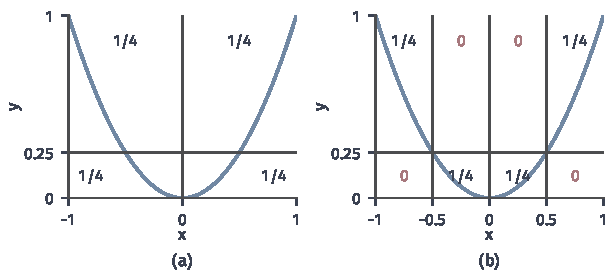
\includegraphics[width=104mm]{figures/07-probability/04-distribution-analysis/matplotlib/dep-partition-grids/figure.pdf}
  \caption{连续抛物线$y=x^{2}$（蓝）在两个固定划分下的格子概率（深灰线为格子边界）。(a)在$x=0$与$y=1/4$处切开，四个格子概率都是$1/4$，标签互信息为$0$；(b)$X$再在$\pm1/2$处切开，八个格子中四个概率为$0$（红），标签互信息为$\ln2$。}
  \label{fig:dep-partition-grids}
\end{BookInlineFigure}

\paragraph{加细的极限}
沿着一列越来越细的划分，标签互信息单调不减，并且不超过$I(X;Y)$。若这列划分最终能分辨所有可测集（例如实轴上以二进端点逐次对分），标签互信息的极限就是$I(X;Y)$；更一般地，互信息等于所有有限划分上标签互信息的上确界\scite{math-cover2006information}。这给出了互信息的另一种读法，也说明了离散化是“从下方逼近”。

在两个边缘都按$k$个等概率区间切分（$k\times k$网格）时，两个例子表现完全不同。对$\rho=0.5$的标准二元高斯，$k=2$时四个格子由象限概率决定，
\[
  \mathbb{P}(X>0,\,Y>0)=\frac14+\frac{\arcsin\rho}{2\pi}=\frac14+\frac{1}{12}=\frac13,
\]
概率表为
\[
  \begin{pmatrix}1/3&1/6\\1/6&1/3\end{pmatrix},\qquad I_2=\tfrac23\ln\tfrac43+\tfrac13\ln\tfrac23\approx0.0566 .
\]
$k$增大时$I_k$迅速上升，$k=8$约为$0.127$，$k=32$约为$0.141$，逼近$0.144$。对连续抛物线，$X$的$k$个等概率区间长为$2/k$，$Y$的$k$个等概率区间对应$\lvert X\rvert$上长为$1/k$的区间。$k$为偶数时，每个$X$格子恰好覆盖两个$Y$格子，且在其中各占一半，所以
\[
  I_k=H\bigl(\beta(Y)\bigr)-H\bigl(\beta(Y)\mid\alpha(X)\bigr)=\ln k-\ln2=\ln\tfrac{k}{2}.
\]
它随$k$无界增长，与定理~\ref{thm:dep-mi-infinite}的无穷大一致；$k=2$给出$0$，正是上面的反例。图~\ref{fig:dep-binned-mi}画出这两条序列。

\begin{BookInlineFigure}
  \centering
  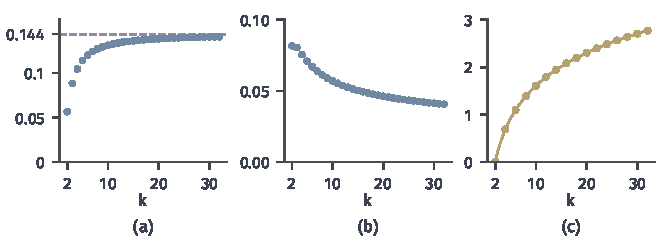
\includegraphics[width=112mm]{figures/07-probability/04-distribution-analysis/matplotlib/dep-binned-mi/figure.pdf}
  \caption{等概率$k\times k$网格上的标签互信息。(a)$\rho=0.5$的标准二元高斯，$I_k$（蓝点）单调上升，逼近紫色虚线$I=0.144$；(b)同一序列除以$\ln k$；(c)连续抛物线，$I_k=\ln(k/2)$（黄，偶数$k$；脚本对$k=4,8$另行数值核对），无界增长。}
  \label{fig:dep-binned-mi}
\end{BookInlineFigure}

\subsection{网格评分}
\label{sec:dep-grid-score}

固定的划分可能恰好错过依赖，自然的补救是在许多划分中搜索，取最能显示关联的那一个。可是互信息随格子数增长，格子越多越占便宜，比较不同大小的网格之前要先归一化。

对实值的$X,Y$，称把$X$的范围切成$k$个区间、$Y$切成$l$个区间所得的划分为一个$k\times l$网格$G$，标签互信息记为$I_G$。标签分别只有$k$与$l$种取值，所以
\[
  I_G\leq\min\bigl(H(\alpha(X)),H(\beta(Y))\bigr)\leq\ln\min(k,l).
\]
于是归一化的比值落在$[0,1]$中。给定格子预算$b\geq4$，定义总体的\term{网格评分}（grid score）
\begin{equation}
  S_b(X,Y)=\sup\Bigl\{\frac{I_G}{\ln\min(k,l)}:\ G\text{为}k\times l\text{网格},\ k,l\geq2,\ kl\leq b\Bigr\}.
  \label{eq:dep-grid-score}
\end{equation}
上确界取遍所有切点位置。令预算$b\to\infty$，得到的总体量就是Reshef等人的\term{最大信息系数}（maximal information coefficient），简称MIC\scite{math-reshef2016dependence}。

\paragraph{零值与确定关系}
总体网格评分的两端可以直接验证。若$X,Y$独立，每个网格的标签都独立，$I_G=0$，评分为零。反过来，若某个预算下评分为零，则所有$2\times2$网格的标签都独立；在$(a,c)$处切开的$2\times2$网格独立，意味着
\[
  \mathbb{P}(X\leq a,\,Y\leq c)=\mathbb{P}(X\leq a)\,\mathbb{P}(Y\leq c),
\]
它对一切$a,c$成立，联合分布函数分解，$X$与$Y$独立。所以只要允许任意切点，网格评分的零值也刻画独立；正是搜索弥补了单个固定划分的缺陷。

另一端，若$Y=f(X)$，$f$在有限个区间上分段连续且单调，$Y$的分布函数连续，则评分在足够大的预算下等于$1$。把$Y$按$l$个等概率区间切分，标签熵为$\ln l$；在单调段的端点与各$Y$切点的原像处切开$X$，每个$Y$格子的原像就是若干个$X$格子之并（对抛物线，取$X$的$2l$个区间即可），这时$Y$的标签由$X$的标签确定，$I_G=\ln l$，而$\min(k,l)=l$，比值为$1$。这与互信息给出$+\infty$形成对照：归一化把“确定关系”压到了上界$1$。

\paragraph{归一化与预算改变刻度}
评分的数值依赖于归一化规则和预算。图~\ref{fig:dep-binned-mi}(b)已经显示，对同一个高斯分布，等概率网格上的$I_k/\ln k$从$k=2$的$0.082$降到$k=32$的$0.041$：分子收敛到$0.144$，分母却继续增长。所以在不同的预算下、或者把分母换成$\ln k$或$\ln(kl)$，得到的是不同的刻度。MIC式的评分把高斯（$I=0.144$）放在$0$与$1$之间某处，把任意无噪声的函数关系都放在$1$，它衡量的是“网格能把关系捕捉得多完整”，不是信息量本身。

\paragraph{总体评分与经验评分}
实际使用时，评分是在一组样本上算的：用$n$个点的经验分布代替联合分布，在预算$b(n)$（常取$n^{0.6}$）以内搜索网格。这样得到的经验评分是另一个对象。即使两个变量独立，有限样本的经验表也不会恰好分解，经验互信息大于零；在许多网格上取最大值，又进一步把偏差放大。

图~\ref{fig:dep-grid-score-sample}用模拟说明这一点。为便于计算，这里只在等频网格中搜索，不优化切点位置，因此它低估了完整搜索的放大效应。对独立的均匀变量，$n=20$时经验评分的平均值约为$0.12$，$95\%$分位数约$0.28$；$n=2560$时平均值降到约$0.019$。对$Y=X^{2}+0.2Z$，$n=20$时经验评分的$5\%$分位数只有约$0.08$，低于独立变量的$95\%$分位数。小样本下两个分布的经验评分大量重叠：一个较高的经验分数，可能只是独立变量在有限样本上的波动。

\begin{BookInlineFigure}
  \centering
  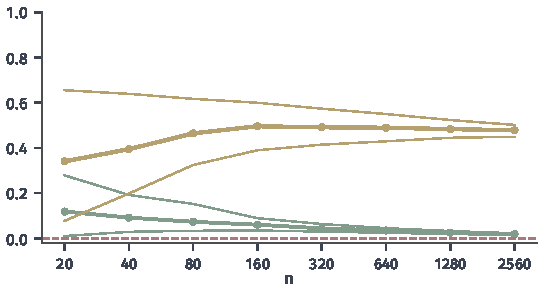
\includegraphics[width=92mm]{figures/07-probability/04-distribution-analysis/matplotlib/dep-grid-score-sample/figure.pdf}
  \caption{经验网格评分随样本量$n$的变化（横轴为对数刻度）。评分在$k,l\geq2$、$kl\leq n^{0.6}$的等频网格上取经验标签互信息除以$\ln\min(k,l)$的最大值。绿：独立的$\operatorname{Unif}(0,1)$对，总体评分为$0$（红色虚线）；黄：$X\sim\operatorname{Unif}(-1,1)$，$Y=X^{2}+0.2Z$。粗线为$200$次重复的平均，细线为$5\%$与$95\%$分位数。种子$719$。}
  \label{fig:dep-grid-score-sample}
\end{BookInlineFigure}

总体网格评分是联合分布的一个确定的泛函；经验评分是样本的函数，带有随机性和偏差。经验网格上的高分，不是“总体关系已经被可靠识别”的证明。要把经验分数变成关于总体的结论，需要分析它在独立假设下的分布并控制多次搜索带来的偏差，这是假设检验的任务，可参考\BookChapterRef{chap:confidence-sets-hypothesis-testing}{卷八第6章“置信集合与假设检验”}。


\section{度量的比较}
\label{sec:dep-comparison}

四类度量都从同一个问题出发：$P_{(X,Y)}$与$P_X\otimes P_Y$相差多少。它们在条件、零值、变换与刻度上的差别，决定了各自适合回答什么。

\paragraph{性质对照}
表~\ref{tab:dep-properties}把前面各节的结论放在一起。“零值刻画独立”一栏都是在所列条件下成立的；HSIC一栏指高斯核或其他使乘积核成为特征核的选择，线性核单独列出作为对照。

\begin{BookInlineTable}
  \centering
  \small
  \begin{tabular}{@{}p{15mm}p{22mm}p{13mm}p{26mm}p{20mm}@{}}
    \toprule
    度量 & 适用条件 & 零值刻画独立 & 保持不变的变换 & 取值与参数\\
    \midrule
    互信息 & 任意可测空间 & 是 & 双向可测一一映射 & $[0,\infty]$，无参数\\
    距离相关 & 欧氏空间，一阶矩 & 是 & 平移、正交、整体缩放 & $[0,1]$，无参数\\
    HSIC（高斯核） & 欧氏空间，无矩条件 & 是 & 平移、正交 & 非负，依赖带宽\\
    HSIC（线性核） & 实值，二阶矩 & 否 & 平移 & $\operatorname{Cov}^{2}$\\
    网格评分 & 实值，任意切点 & 是 & 严格增变换 & $[0,1]$，依赖预算\\
    \bottomrule
  \end{tabular}
  \caption{依赖度量的性质对照。“保持不变的变换”指对两个变量分别作该类变换时度量不变；HSIC在整体缩放下数值改变，除非带宽随之缩放。网格评分只依赖切点两侧的概率，严格增变换只移动切点，不改变可达到的概率表。}
  \label{tab:dep-properties}
\end{BookInlineTable}

表中的三列各自对应第一节的一件事。零值一栏回答“能否判断独立”，除线性核外答案都是肯定的，条件却不同：互信息不要求任何结构，距离相关要一阶矩，HSIC要合适的核，网格评分要求实值并允许任意切点。后两栏回答“非零数值有什么含义”，这里没有两种度量完全一致。

\paragraph{同一组分布上的数值}
表~\ref{tab:dep-values}列出本章几个例子的数值。互信息以nat为单位；HSIC用带宽为$1$的高斯核。

\begin{BookInlineTable}
  \centering
  \small
  \begin{tabular}{@{}lcccc@{}}
    \toprule
    联合分布 & 相关系数 & 互信息 & 距离相关 & HSIC\\
    \midrule
    三点抛物线 & $0$ & $0.637$ & $0.562$ & $0.0138$\\
    连续抛物线 & $0$ & $+\infty$ & $0.491$ & $0.0026$\\
    $Y=X^{2}+0.1Z$ & $0$ & $1.03$ & $0.461$ & $0.0026$\\
    高斯，$\rho=0.5$ & $0.5$ & $0.144$ & $0.454$ & $0.0108$\\
    高斯，$\rho=0.6$ & $0.6$ & $0.223$ & $0.550$ & $0.0166$\\
    \bottomrule
  \end{tabular}
  \caption{本章例子的依赖度量。连续抛物线与$Y=X^{2}+0.1Z$中$X\sim\operatorname{Unif}(-1,1)$，距离相关与HSIC由对$X$的数值积分得到；高斯的互信息由式~\eqref{eq:dep-gauss-mi}，距离相关由闭式，HSIC由式~\eqref{eq:dep-hsic-gauss}。}
  \label{tab:dep-values}
\end{BookInlineTable}

表中的相关系数在三个抛物线例子上都是零，其余三个度量都识别出了依赖。非零数值的次序则各不相同。比较$\rho=0.6$的高斯与$Y=X^{2}+0.1Z$：互信息说后者的依赖强得多（$1.03$对$0.223$），距离相关说前者更强（$0.550$对$0.461$）。图~\ref{fig:dep-ranking}画出这两个分布的样本。

\begin{BookInlineFigure}
  \centering
  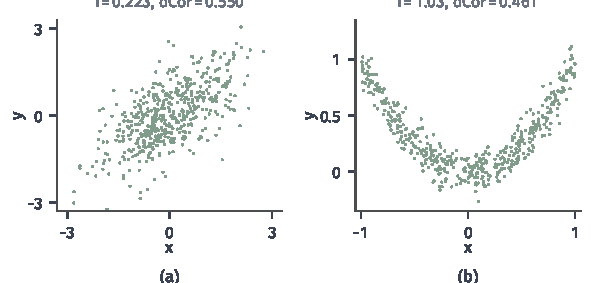
\includegraphics[width=100mm]{figures/07-probability/04-distribution-analysis/matplotlib/dep-ranking/figure.pdf}
  \caption{两个依赖度量给出相反次序的一对分布，各$500$个样本（绿，种子$719$）。(a)$\rho=0.6$的标准二元高斯；(b)$X\sim\operatorname{Unif}(-1,1)$，$Y=X^{2}+0.1Z$。图上方是总体互信息（nat）与距离相关：互信息认为(b)更强，距离相关认为(a)更强。}
  \label{fig:dep-ranking}
\end{BookInlineFigure}

两种判断都有道理，它们回答的是不同的问题。(b)中知道$X$以后，$Y$被限制在抛物线附近宽约$0.1$的窄带里，不确定性大幅减少，所以互信息大。但$X$的一对取值相距远时，$Y$的一对取值未必相距远：$X=\pm0.8$相距$1.6$，对应的$Y$几乎相同。距离相关问的是距离的同步，抛物线的折返削弱了这种同步，所以它更小。HSIC的次序还要看带宽：若两个坐标的带宽都取$1$，表~\ref{tab:dep-values}中高斯更大；若带宽取各坐标的标准差，(b)的HSIC约为$0.0286$，(a)约为$0.0166$，次序又与互信息一致。

\paragraph{真实值与可计算的下界}
互信息还有一个使用上的问题。连续抛物线的互信息是$+\infty$，$\sigma=0.1$的含噪抛物线是$1.03$，而数值方法得到的常常只是一个下界。第~\ref{chap:information-measures}章的InfoNCE下界在$N$个候选时不超过$\ln N$，候选数或评分函数的限制会让下界远低于真实值，并且对不同分布低估的程度不同。比较两个分布的互信息时，要比较的是真实值；拿两个下界的大小作比较，次序可能与真实值相反。

\paragraph{选择依赖度量}
没有一个度量能脱离任务给出统一的强度刻度。若关心的是一个变量能为另一个提供多少信息，且希望结果不受坐标和单位影响，用互信息，并准备好处理无穷大与估计困难。若变量是欧氏空间中的向量，希望用距离和有界的数值描述“取值是否一起变化”，用距离相关，并先统一各坐标的单位。

若变量取值于一般空间（文本、图、函数），或需要在特定尺度上检查依赖，用HSIC，并把核与带宽作为结论的一部分报告。若希望在给定分辨率下读出一张可解释的概率表，用离散化评分，并说明划分方式与归一化规则。几种量能同时判别独立，却可能给出不同的非零排序，选择之前先说清楚要比较的是哪一种依赖。


\section{本章小结}
\label{sec:dep-summary}

本章从$X\sim\operatorname{Unif}(-1,1)$与$Y=X^{2}$出发：协方差为零，依赖却是确定的。协方差只检查一对线性函数，独立要求联合分布等于边缘乘积，即对所有有界函数对乘积公式都成立。依赖度量就是对这一差别的量化，评价它时要分开三件事：零值是否刻画独立，非零数值随依赖怎样变化，以及能否从有限样本可靠判断。本章只讨论前两件。

互信息是联合分布相对边缘乘积的KL散度，零值在任何可测空间上刻画独立。它在双向可测的一一变换下不变，在不可逆的局部处理下不增，连续边缘时只依赖Copula。它不看取值之间的距离，也没有有限上界：在标准Borel空间上，只要$Y=f(X)$且$Y$的分布无原子，联合分布就集中在边缘乘积给零概率的图像上，互信息为无穷大。有限的计算下界不等于真实值。

距离协方差用权重$\lVert\bm{t}\rVert_2^{-(p+1)}\lVert\bm{s}\rVert_2^{-(q+1)}$对特征函数之差作平方积分。一阶矩保证它有限，零值由特征函数的唯一性刻画独立。二阶矩有限时它等于成对距离的三项期望，也等于双重中心化距离乘积的期望；中心化消去了只由边缘决定的部分，而指数$1$（不是$2$）使它看到非线性依赖。用距离方差归一化得到取值于$[0,1]$的距离相关，它在平移、正交变换和整体缩放下不变，取$1$当且仅当两组坐标只差一个相似变换，常量情形约定为$0$。

HSIC是联合分布与边缘乘积在乘积核下的平方MMD，等于核期望的三项组合，也等于交叉协方差算子的Hilbert--Schmidt范数平方。乘积核为特征核时零值刻画独立，高斯核满足这一条件；线性核只剩协方差的平方，距离诱导核给出距离协方差的四分之一。高斯核的带宽改变数值，甚至改变两个分布的次序。

离散化评分把取值装进有限个格子。固定划分的标签互信息不超过原互信息，可能恰好错过依赖；沿加细的划分它逼近互信息。在允许任意切点的网格中搜索并按$\ln\min(k,l)$归一化，总体评分的零值刻画实值变量的独立，分段单调的无噪声函数关系得分为$1$。经验网格评分是样本的函数，小样本下对独立变量也会给出明显的正值。

这些量能同时判别独立，却按不同的方式度量依赖：互信息量信息的减少，距离相关量距离的同步，HSIC量指定尺度上的特征协方差，网格评分量网格能否捕捉关系。选择之前要说清楚随机对象所在的空间、可积条件、需要保持的变换，并把零值判别与非零强度比较分开。用样本估计这些量、校准估计误差和检验独立性，由卷八的非参数推断与假设检验两章承接；算出一个样本分数，并不等于完成了统计判断。


